% kate: word-wrap true;

% IMPORTANT NOTE: I've never dealt much with syntax before, at least not in a
% way as formal as I'm trying to come to terms with it here. If there's
% anything wrong with my analyses, it's because I don't know enough yet. Things
% may be subject to change *especially* in this chapter.

\chapter{Phrase structures}
\label{ch:phrasestruct}

While the previous chapter dealt largely with the various parts of speech and
their various distributive and inflectional properties, the present chapter
will elaborate on how these words combine into syntactic phrases.\footnote{It
should be noted that, since trees are large, a number of regularly numbered
examples in this chapter will appear not in place but floated, like tables and
figures in the previous chapters.} Since Ayeri is a verb-initial language, it
is probably most comfortably analyzed in terms of Lexical-Functional Grammar
(\cite{bresnan1982}~ff.; more recently \cite{bresnan2016};
\cite{dalrymple2001}), since \Lfg{} does not require complicated derivations
behind the surface structure of sentences.\footnote{Passivization, for
instance, is assumed to be a lexically motivated alternation in predicate
structure (\Subj{} is prohibited, so the nominative is assigned to \Obj{}, and
the original \Subj{} is expressed  by an \Adjc{}), rather than an internal
derivational process \citep[23\psqq]{bresnan2016}.} It will be assumed here
that, even though Ayeri is basically VSO with predicate and predication not
adjacent to each other, it is configurational in that there is a VP which
c-commands a number of other constituents as complements in transitive
sentences.

In principle, \Lfg{} assumes that grammar operates on different structural 
levels: mainly, these are a(rgument) structure, c(onstituent) structure, and 
f(unctional) structure; other layers have been proposed by different 
researchers for different purposes \citep[862--865]{buttking2015}. 
\citet{bresnan2016} define three core design principles for \Lfg{}:

\begin{description}
\item[Variability:] \textcquote[41]{bresnan2016}{The principle of variability
states that \emph{external structures vary across languages}. The formal model
of external structure in \Lfg{} is the \emph{c-structure}, which stands for
\enquote{constituent structure} or \enquote{categorial structure}}. 
C-structures are commonly represented by context-free phrase-structure rules; 
constituency trees are based on an extended version of X-bar theory 
\citep[42]{bresnan2016}.\footnote{The basic recursive rules of X-bar theory 
are observed:
\begin{enumerate}[nosep, leftmargin={2\footnotemargin}]
\item XP → YP, \xbar{X} (specifier rule)
\item \xbar{X} → \xbar{X}, ZP (adjunct rule)
\item \xbar{X} → \xhead{X}, WP (complement rule)
\end{enumerate}

The principle of economy of expression furthermore dictates that essentially,
trees be pruned of empty terminal nodes and non-branching preterminal nodes,
since these do not provide structurally or semantically relevant information
\citep[119--128]{bresnan2016}. Thus, for instance, in a rule like XP →
\xhead{X} YP, YP is not necesssarily XP's complement. Functional annotations on
nodes will clarify their status instead of their position in a c-structure
tree.}

\item[Universality:] \textcquote[42]{bresnan2016}{The principle of universality
states that \emph{internal structures are largely invariant across languages}.
The formal model of internal structure in \Lfg{} is the \emph{f-structure},
which stands for \enquote{functional structure}}. The f-structure is depicted
as an argument-value matrix (\Avm{}) which maps the relations between `subject'
(\Subj{}), `object' (\Obj{}), `predicator' (\Pred{}), etc.\ as functional
abstractions of NP, VP, V, etc.\ \citep[42]{bresnan2016}. Verbs are also
presented with their \fw{a-structure} spelled out. That is, which arguments a
verb has relations to is formally stated \citep[15]{bresnan2016}. The
f-structure collates semantic features associated with heads of grammatical
functions (GFs), such as case (\Case{}), person (\Pers{}), number (\Num{}),
which are abstract features and as such need not have morphological realization
\citep[43]{bresnan2016}.

\item[Monotonicity:] \textcquote[43]{bresnan2016}{Constituent structure form is
simply not the same in all languages [...] In \Lfg{} the correspondence mapping
between internal and external structures does not preserve sameness of form.
Instead, \emph{it is designed to preserve inclusion relations between the
information expressed by the external structure and the content of the internal
structure}}. Due to the principle of monorepresentation, information
distributed over different morphemes which logically belongs to a single
grammatical function is presented in the f-structure as unified.

\end{description}

\begin{figure}[t]\centering
\begin{tabular}[t]{l @{\quad\quad} c}
argument (a-)structure:
& \astruct{\tikzmark{verb}verb}{\tikzmark{x}x, \tikzmark{y}y}\bigskip \\

functional (f-)strucutre:
& \tikzmark{fstruct}{\smaller\begin{avm}
\[
	\quad sbj \tikzmark{subj} & \[
		{\enspace}\vdots{\enspace} \\
	\]{\quad} \\
	\quad obj \tikzmark{obj} & \[
		{\enspace}\vdots{\enspace} \\
	\] \tikzmark{objval}{\quad} \\
	\quad \tikzmark{pred} pred & \dots \tikzmark{predval} \\
\]
\end{avm}}\bigskip\\

constituent (c-)structure:
& \begin{forest} baseline
[\xbar{V}
	[\subnode{V}{V}]
	[NP \tikzmark{NP}
		[\xbar{N} \tikzmark{Nbar}]
	]
]
\end{forest}
%
\end{tabular}
\begin{tikzpicture}[remember picture, overlay]
\draw [-latex]
	([xshift=1.5ex, yshift=-0.5ex]{pic cs:verb})
	to [out=south, in=north west]
	([yshift=1ex]{pic cs:pred});
\draw [-latex]
	([xshift=0.5ex, yshift=-0.5ex]{pic cs:x})
	to [out=south, in=north east]
	([yshift=1ex]{pic cs:subj});
\draw [-latex]
	([xshift=0.5ex, yshift=-0.75ex]{pic cs:y})
	to [out=south, in=north east]
	([yshift=1ex]{pic cs:obj});
\draw [-latex]
	([yshift=1ex]{pic cs:V})
	to [out=west, in=south west]
	([yshift=-10ex]{pic cs:fstruct});
\draw [-latex]
	([yshift=1ex]{pic cs:NP})
	to [out=east, in=east]
	([yshift=1ex]{pic cs:objval});
\draw [-latex]
	([yshift=1ex]{pic cs:Nbar})
	to [out=east, in=east]
	([yshift=1ex]{pic cs:objval});
\end{tikzpicture}
\caption[F-structure mappings]{F-structure mappings \citep[15]{bresnan2016}}
\label{fig:phimap}
\end{figure}

To illustrate the different parallel structures in operation,
\citet[15]{bresnan2016} give the schema in \autoref{fig:phimap} to demonstrate
which part of the a- and c-structure respectively corresponds (`links', `maps')
to which part of the f-structure.
% \footnote{\citet{bresnan2016} use \textsc{`subj'} for `subject'. ; for
% consistency with the above I will use `\Subj{}' in the following. I will also
% divergently use \Compl{} and \XCompl{} for \textsc{(x)comp}, since
% \textsc{comp} has already been used for `comparative' above.}
Regarding the different functions distinguished, \Lfg{} 
assumes the following hierarchies \citep[97, 100]{bresnan2016}:

\pex\label{ex:functions}
\a\label{ex:gfs} Grammatical functions (\GF{}s):\\
	$\overbrace{\Subj{} > \Obj{} > \SObj{}}^{\text{core}} > 
	\overbrace{\Oblique{} > \XCompl{}, \Compl{} > \Adjc{}}^{\text{noncore}}$
\a\label{ex:nonafs} (Non)argument functions (\AF{}s/$\overline{\mbox{\AF{}}%
}$s):\\
	$\underbrace{\Top{}\: \Foc{}}_{\text{non-a-fns}}\; 
	\overbrace{\Subj{}\: \Obj{}\: \SObj{}\: \Oblique{}\: \XCompl{}\: 
		\Compl{}}^{\text{a-fns}}\; 
	\underbrace{\Adjc{}}_{\text{non-a-fns}}$
\a\label{ex:dfs} Discourse functions (\DF{}s):\\
	$\overbrace{\Top{}\: \Foc{}\: \Subj{}}^{\text{d-fns}}\;
	\underbrace{\Obj{}\: \SObj{}\: \Oblique{}\: \XCompl{}\: \Compl{}\: 
		\Adjc{}}_{\text{non-d-fns}}$
\xe

The elements listed in (\ref{ex:functions}) will also appear in
phrase-structure rules and c-structure trees together with arrows. These arrows
symbolize inheritance of feature information from the current level (↓) of the
tree to the next (↑), so for instance, `\pass{\Subj}' means that the information
subsumed by the current node (`down') is passed on as the subject function of
the next higher node (`up') in the tree. Concise information on notational
formalisms of \Lfg{} can be found, for instance, in \citet{buttking2015}.

\section{Noun and determiner phrases}
\label{sec:nps-dps}

Noun phrases (NPs), and determiner phrases (DPs) as their functional 
counterpart, fulfill the functions of subject (\Subj{}), object (\Obj{}), 
secondary object (\SObj{}), as well as various oblique constituents (\Oblique;
see (\ref{ex:dpnpcasemap}) below), and they can also form adjuncts (\Adjc{}).
DPs and NPs can also constitute topics (\Top{}). Which DP or NP receives which 
function is selected by the a-structure of the verb---this also has 
repercussions on case- and topic marking.

Since the constituent containing the various non-verbal elements in Ayeri is 
likely exocentric and constituents may move around within it in a restricted 
way, we have to assume that not constituent structure, but case marking 
identifies the grammatical functions of the various arguments of verbs. Thus, 
the following lexicocentric conditions operate on both DP and NP as exponents 
of case:

\ex\label{ex:dpnpcasemap}\labels
\begin{tabular}[t]{@{} l @{\quad} l @{ $\implies$ } l}
\tl\quad & \downs{\Case} = \Aarg	& \pass{\Subj} \\
\tl\quad & \downs{\Case} = \Parg	& \pass{\Obj} \\
\tl\quad & \downs{\Case} = \Dat		& \pass{\SObj} \logor{}
%	\pass{\Oblq{goal}} \\
	\ups{\PCase} = \Oblq{goal} \\
\tl\quad & \downs{\Case} = \Gen		& \pass{\Possr} \logor{} 
%	\pass{\Oblq{src}} \\
	\ups{\PCase} = \Oblq{src} \\
\tl\quad & \downs{\Case} = \Loc		& \pass{\Oblq{loc}} \logor{}
	\ups{\PCase} = \Oblq{loc} \\
\tl\quad & \downs{\Case} = \Caus	& \pass{\Oblq{caus}} \\
\tl\quad & \downs{\Case} = \Ins		& \pass{\Oblq{ins}} \\
\end{tabular}
\xe

The rules in (\ref{ex:dpnpcasemap}) determine the typical mappings between case
marking and grammatical functions, which are not always unambiguous. As
explained above (compare \autoref{subsec:case}), the dative case does not only
indicate that something is done to this referent or to their benefit, but it
may also indicate motion towards this referent. Likewise, the genitive case
does not only indicate possession, but also origin, and motion from this
referent. Nominal adjuncts to nouns which specify what the noun consists also
appear in the instrumental case, besides the instrumental being used to
indicate the means or the circumstance by which an action comes about.
Moreover, DPs or NPs may also lack case marking, which indicates that the
respective phrase is a part of the topic of the verb, which is what
(\ref{ex:topicrule}) describes:

\ex\label{ex:topicrule}
¬\,\downs{\Case} $\implies$ \elem{\Top}
\xe

Instead of case marking on the DP or NP, there is a marker in front of the verb
which provides information on the case and, if \AgtT{} or \PatT{}, also about
the animacy of the topicalized phrase. This means that grammatical information
about the topic of a phrase is spread over two discontinuous locations. This
issue does not pose a problem to an \Lfg{}-based analysis, however, since both
locations unify their information content in the f-structure feature \Top{}.
Since information located in multiple places is jointly feeding this feature, I
am using the annotation `\elem{\Top}' for each location rather than simple
`\pass{\Top}'. Note that only one NP among the arguments of a verb may be the
topic of the phrase, and a topic can only be marked if the verb is finite and
the number of arguments to the verb is greater than one.

\subsection{Noun phrases}
\label{subsec:nps}

\subsubsection{Constituent order within noun phrases}

Nouns are one of the main parts of speech of Ayeri, and nouns can be modified
by a number of other free elements, as we have seen previously---adjectives,
possessive adjectives, as well as relative clauses and nominal adjuncts. These
typically follow nouns. It was also described before that Ayeri's nouns may
host a number of clitics, among which are deictic prefixes and quantifiers, as
well as enclitic case markers in the case of proper nouns. These clitics,
however, will not be treated as targets of syntactic operations, since \Lfg{}
follows the approach of lexical integrity. Thus, bound elements like affixes
and clitics are assumed not to be reflected or affected by syntax itself. The
phrase structure of NPs should thus look like depicted in (\ref{ex:npstruct}).
The asterisk in (\ref{ex:npstruct_Adj}) is the Kleene star and indicates zero
or more instances of the element. Elements which may be omitted or occur once
are in brackets.

\pex\label{ex:npstruct}
\a NP → \anno*{\xbar{N}} $\left(\anno*[\pass{\Compl}]{CP}\right)$
\a \xbar{N} → \anno*{\xbar{N}} $\left(\anno*[\pass{\Possr}]
	{\{NP | DP\}}\right)$
\a \xbar{N} → \anno*{\xbar{N}} $\left(\anno*[\pass{\Compl}]{NP}\right)$
\a\label{ex:npstruct_Adj}%
	\xbar{N} → \anno*{\xhead{N}} \anno*[{\elem{\Adjc}}]{AP*}
\xe

This rule defines that NPs have a lexical head which is on the left side,
followed optionally by modifiers which may have various relationships to the
noun: complement (instrumental nominal, NP/DP), adjunct (adjective phrase, AP),
possessor (genitive NP/DP), relative clause (forming a complementizer phrase,
CP). This can be represented as a constituent-structure tree in the way
described in (\ref{ex:npcstruct}).

\begin{figure}
\ex\label{ex:npcstruct}\labels
\begin{forest} shorter edges,
[{\anno[\{\pass{\DF} | \pass{\GF}\}]{NP}}
%	[\anno{\xbar{N}}
		[\anno{\xbar{N}}
			[\anno{\xbar{N}}
				[\anno{\xbar{N}}
					[\anno{\xhead{N}}]
					[{\anno[\elem{\Adjc}]{AP*}}]
				]
				[{$\left(\anno[\pass{\Compl}]{XP}\right)$}]
			]
			[{$\left(\anno[\pass{\Possr}]{\{NP | DP\}}\right)$}]
		]
		[{$\left(\anno[\pass{\Compl}]{CP}\right)$}]
%	]
]
\end{forest}
\xe
\end{figure}

In (\ref{ex:npcstruct}) as well, we can see a nominal head on the left which
may be modified by phrases of various types. The maximal projection of
\xhead{N} (that is, NP) is annotated very generally for the function of the
NP---basically, an NP can act as either a discourse function (\DF{}) or a
grammatical function (\GF{}). (\ref{ex:nounmods}) gives an example of each kind
of modifier. Since there is no grammatical context given, NP is unmarked for
function in these examples.

\begin{figure}
\pex\label{ex:nounmods}
\a %
	\begin{minipage}[t]{.5\remaining}
	\begingl
		\glpreamble noun + adjective: //
		\gla ningan hiro //
		\glb ningan hiro //
		\glc story new //
		\glft `new story' //
	\endgl
	\end{minipage}
	~
	\begin{forest} shorter edges, italic leaves,
	[NP
%		[\anno{\xbar{N}}
			[\anno{\xhead{N}}
				[{ningan}]
			]
			[{\anno[\elem{\Adjc}]{AP}}
				[{hiro}, roof]
			]
%		]
	]
	\end{forest}

\a %
	\begin{minipage}[t]{.5\remaining}
	\begingl
		\glpreamble noun + possessor: //
		\gla kegan ayonena //
		\glb kegan ayon-ena //
		\glc hat man-\Gen{} //
		\glft `the man's hat' //
	\endgl
	\end{minipage}
	~
	\begin{forest} shorter edges, italic leaves,
	[NP
%		[\anno{\xbar{N}}
			[\anno{\xhead{N}}
				[{kegan}]
			]
			[{\anno[\pass{\Possr}]{NP}}
				[{ayonena}, roof]
			]
%		]
	]
	\end{forest}

\a %
	\begin{minipage}[t]{.5\remaining}
	\begingl
		\glpreamble noun + instrumental complement: //
		\gla kasu bariri //
		\glb kasu bari-ri //
		\glc basket meat-\Ins{} //
		\glft `basket of meat' //
	\endgl
	\end{minipage}
	~
	\begin{forest} shorter edges, italic leaves,
	[NP
%		[\anno{\xbar{N}}
			[\anno{\xhead{N}}
				[{kasu}]
			]
			[{\anno[\pass{\Compl}]{NP}}
				[{bariri}, roof]
			]
%		]
	]
	\end{forest}

\a %
	\begin{minipage}[t]{.5\remaining}
	\begingl
		\glpreamble noun + relative clause: //
		\gla nanga si incāng //
		\glb nanga si int=yāng //
		\glc house \Rel{} buy=\TsgM{}.\Aarg{} //
		\glft `the house he bought' //
	\endgl
	\end{minipage}
	~
	\begin{forest} shorter edges, italic leaves,
	[NP
%		[\anno{\xbar{N}}
			[\anno{\xhead{N}}
				[{nanga}]
			]
			[{\anno[\pass{\Compl}]{CP}}
				[{si incāng}, roof]
			]
%		]
	]
	\end{forest}

\xe
\end{figure}

As described before (compare \autoref{subsec:clitics}), nouns can be modified
by a number of clitics which are not represented through syntax. Since it is
not possible for these clitic elements to be divided from their phonological
hosts, they should be treated as being an integral part of the word they attach
to. Hence, \xhead{N} is given in (\ref{ex:nouncltree}) as split into `Cl' and
\xhead{N}.

\begin{figure}
\pex\label{ex:nouncltree}
\a %
	\begin{minipage}[t]{.5\remaining}
	\begingl
		\glpreamble noun + deictic prefix: //
		\gla eda- @ nanga //
		\glb eda= nanga //
		\glc this= house //
		\glft `this house' //
	\endgl
	\end{minipage}
	~
	\begin{forest} shorter edges, italic leaves,
	[\anno{\xhead{N}}
		[\anno{Cl}
			[eda-]
		]
		[\anno{\xhead{N}}
			[nanga]
		]
	]
	\end{forest}

\a %
	\begin{minipage}[t]{.5\remaining}
	\begingl
		\glpreamble noun + quantifier: //
		\gla nangās @ -ikan //
		\glb nanga-as =ikan //
		\glc house-\Parg{} =many //
		\glft `many houses' //
	\endgl
	\end{minipage}
	~
	\begin{forest} shorter edges, italic leaves,
	[\anno{\xhead{N}}
		[\anno{\xhead{N}}
			[nangās]
		]
		[\anno{Cl}
			[-ikan]
		]
	]
	\end{forest}

\a %
	\begin{minipage}[t]{.5\remaining}
	\begingl
		\glpreamble proper noun + case: //
		\gla ang @ Diyan //
		\glb ang= Diyan //
		\glc \Aarg{}= Diyan //
		\glft `Diyan' //
	\endgl
	\end{minipage}
	~
	\begin{forest} shorter edges, italic leaves,
	[\anno{\xhead{N}}
		[\anno{Cl}
			[ang]
		]
		[\anno{\xhead{N}}
			[Diyan]
		]
	]
	\end{forest}

\xe
\end{figure}

Of course, it is also possible to combine these nominal modifiers. In this
case, there is a certain hierarchy, presumably based on Behaghel's first law,
\textquote{Das oberste Gesetz ist dieses, daß das geistig eng Zusammengehörige 
auch eng zusammengestellt wird} (\cite[4]{behaghel1932}; `The supreme law is
such that the mentally closely related is also arranged in close proximity.'), 
and also grammatical weight \citep{wasow1997}:

\begin{enumerate}[noitemsep]
	\item instrumental NP indicating what the head consists of,
	\item APs (also cardinals) and other NPs describing attributes,
	\item possessive genitive NPs,
	\item relative clauses.
\end{enumerate}

\citet{wasow1997} writes that \textcquote[102]{wasow1997}{[i]t is very hard to
distinguish among various structural weight measures as predictors of weight
effects. Counting words, nodes, or phrasal nodes all work well}, which means
that no single metric can be used to describe the order of constituents in a
phrase. However, for instance, relative clauses trail whenever possible
presumably since they tend to contain whole subclauses and thus a lot of
information. It seems advisable not to put an element with much less
information content after them, especially when it refers to a different head
than all the things inside the relative clause. The following example
(\ref{ex:nounmodord}) illustrates the unmarked order of modifiers.

\begin{figure}
\pex\label{ex:nounmodord}
\a\begingl
	\gla diranang caban nā si ang mica ya @ Kārvisam //
	\glb diran-ang caban nā si ang mit=ya.Ø ya= Kārvisam //
	\glc uncle-\Aarg{} favorite \Fsg{}.\Gen{} \Rel{} \AgtT{} 
		live=\TsgM{}.\Top{} \Loc{}= Kārvisam //
	\glft `my favorite uncle who lives in Kārvisam' //
\endgl
\medskip

\a\begin{forest} shorter edges, narrower nodes, italic leaves,
[{\anno[\pass{\Subj}]{NP}}
%	[\anno{\xbar{N}}
		[\anno{\xbar{N}}
			[\anno{\xbar{N}}
				[\anno{\xhead{N}}
					[{diranang}]
				]
				[{\anno[\pass{\Adj}]{AP}}
					[{caban}, roof]
				]
			]
			[{\anno[\pass{\Possr}]{DP}}
				[{nā}, roof]
			]
		]
		[{\anno[\pass{\Comp}]{CP}}
			[{si ang mica ...}, roof]
		]
%	]
]
\end{forest}
\xe
\end{figure}

As the c-structure tree in (\ref{ex:nounmodord}) shows, Ayeri prefers
head--dependent word order with exceeding consistency. As illustrated by
previous examples, both adjuncts and complements are, for the most part,
consistently appended to the right of their heads, which means that Ayeri may
be classified as a rather consistently right-branching language. However, a
certain number of postpositions form an exception to this classification
(\autoref{subsec:postpos}). In the light of word order typology, we can
formulate the following generalizations:

\pex
\a Order of noun and adjective: N Adj
\a Order of noun and genitive: N Gen
\a Order of noun and relative clause: N Rel
\xe

More important to \Lfg{} than c-structure trees, however, are
function-structure matrices which gather all information in a given utterance
and gather potentially disparate information into semantically coherent units
within the matrix.\footnote{Essentially, c-structure is similar to the tree
hierarchy of paragraphs, images, tables etc.\ in an \textsc{html} file, while
f-structure describes semantic properties of elements in the tree similar to
how \textsc{css} defines the layout properties of these elements.} In the
following, I will thus give a list of morpholexic specifications which give an
overview of the different semantic and morphological features nouns basically
provide (also compare \autoref{sec:nouns}). These also form the basis for
f-structure matrices of the kind already shown in (\ref{ex:clitics_43}),
\autoref{clitics_postverb_person}, p.~\pageref{ex:clitics_43}.

\begin{morphlex}
\ex\label{ex:nounmorphlex}%
\adjustbox{valign=t}{%
	\begin{tabu} {\usetabu{morphlexnarrow}}
	...
		& N
		& \begin{tabular}[t]{l l l}
			\ups{\Pred} & = & `...' \\
			\ups{\Anim} & = & $\pm$ \\
			\ups{\Case} & = & \{\Aarg{}, \Parg{}, \Dat{}, \Gen{}, 
				\Loc{}, \Ins{}, \Caus{}\} \\
			\ups{\Gend} & = & \{\M{}, \F{}, \N{}, \Inan{}\} \\
			\ups{\Num} & = & \{\Sg{}, \Pl{}\} \\
			\ups{\Pers} & = & 3 \\
		\end{tabular}
	\end{tabu}%
}
\xe
\end{morphlex}

Nouns generally imply a third-person reference; they distinguish number, gender
and animacy, as well as case. Clitics, however, may also add information about
deixis (\ref{ex:deixisfeat}); likeness and quantity might be interpreted
conveniently as adding to the list of a noun's \Adjc{} feature 
(\ref{ex:nounqadj}).

\begin{morphlex}
\ex\label{ex:deixisfeat}
\adjustbox{valign=t}{%
	\begin{tabu} {\usetabu{morphlexnarrow}}
	\hphantom{...}
		& \hphantom{N}
		& \begin{tabular}[t]{l l l}
			\ups{\Deix} & = & \{$this$, $that$, $such$\} \\
		\end{tabular}
	\end{tabu}%
}
\xe
\end{morphlex}

\begin{figure}
\pex\label{ex:nounqadj}
\a\begingl
	\gla ganang-hen mino //
	\glb gan-ang=hen mino //
	\glc child-\Aarg{}=all happy //
	\glft `all happy children' //
\endgl

\a\begin{avm}
\[
	\Subj{}	&	\[
					\Pred	&	`child' \\
					\Anim	&	$+$ \\
					\Case	&	\Aarg \\
					\Adjc	&	\{
									\[
										\Pred	&	`all' \\
									\], \\
									\[
										\Pred	&	`happy' \\
									\] \\
								\} \\
				\] \\
\]
\end{avm}
\xe
\end{figure}

\subsubsection{Morphosyntactic operations within the noun phrase}

It has been pointed out above that nouns encode animacy. This has repercussions
in the choice of case markers of the agent and patient cases, which need to
agree with the lexical head they attach to. An example of this is given in 
(\ref{ex:animcaseagr}).

\begin{figure}
\ex\label{ex:animcaseagr}\labels
\begin{minipage}[t]{.5\remaining}
\tl\quad\label{ex:animok} %
\begin{forest}
[\anno{\xhead{N}}
	[\anno{N\tsub{stem}}
		[{%
			\textit{gan} \\
			\ups{\Anim} = $+$ \\
		}]
	]
	[\anno{-N\tsub{infl}}
		[{%
			\textit{-ang} \\
			\ups{\Anim} = $+$ \\
			\ups{\Case} = \Aarg{} \\
		}]
	]
]
\end{forest}
\end{minipage}
~
\begin{minipage}[t]{.5\remaining}
\tl\quad\label{ex:animclash} %
\ljudge*\begin{forest}
[\anno{\xhead{N}}
	[\anno{N\tsub{stem}}
		[{%
			\textit{gan} \\
			\ups{\Anim} = $+$ \\
		}]
	]
	[\anno{N\tsub{infl}}
		[{%
			\textit{-reng} \\
			\ups{\Anim} = $-$ \\
			\ups{\Case} = \Aarg{} \\
		}]
	]
]
\end{forest}
\end{minipage}
\xe
\end{figure}

Example (\ref{ex:animcaseagr}a) shows a well-formed construction: the noun,
\xayr{gnF}{gan}{child}, is animate, hence the case particle also needs to be 
animate---the case particle must thus be \rayr{/As}{-ang} to be coherent. In
contrast to this, example (\ref{ex:animcaseagr}b) is not well-formed in that
the noun is animate but the case particle, \rayr{/reNF}{-reng}, signals that it
is inanimate: the \Anim{} values of the noun stem and its suffix clash and
cannot be conclusively unified for \xhead{N} itself. The same principle of
coherence is, of course, also true for proper nouns, which receive a
case-marking particle, as illustrated by (\ref{ex:animcaseagrname}).

\begin{figure}
\ex\label{ex:animcaseagrname}\labels
\begin{minipage}[t]{.5\remaining}
\tl\quad\label{ex:animokname} %
\begin{forest}
[\anno{\xhead{N}}
	[\anno{Cl}
		[{%
			\textit{ang} \\
			\ups{\Anim} = $+$ \\
			\ups{\Case} = \Aarg{} \\
		}]
	]
	[\anno{\xhead{N}}
		[{%
			\textit{Dita} \\
			\ups{\Anim} = $+$ \\
		}]
	]
]
\end{forest}
\end{minipage}
~
\begin{minipage}[t]{.5\remaining}
\tl\quad\label{ex:animclashname} %
\ljudge*\begin{forest}
[\anno{\xhead{N}}
	[\anno{Cl}
		[{%
			\textit{eng} \\
			\ups{\Anim} = $-$ \\
			\ups{\Case} = \Aarg{} \\
		}]
	]
	[\anno{\xhead{N}}
		[{%
			\textit{Dita} \\
			\ups{\Anim} = $+$ \\
		}]
	]
]
\end{forest}
\end{minipage}
\xe
\end{figure}

Furthermore, example (\ref{ex:nounqadj}) already showed that nouns may be
modified by quantifiers, whether these are clitic suffixes
(\autoref{subsec:quantifiers}) or numerals (\autoref{sec:numerals}). In these
cases, plural marking on the noun is suppressed by the presence of the modifier
which supplies the information by itself so that further morphological plural
marking by the suffix \rayr{/ye}{-ye} on the noun stem itself would be
redundant. As shown in \autoref{sec:numerals} (p.~\pageref{hundreds}), however,
there are very limited occasions where a noun may be marked for plural in spite
of the presence of a numeral, for instance as in (\ref{ex:plovermkg}).

\ex\label{ex:plovermkg}\begingl
	\gla Ang bengyon keynamye menang kanānya {desay iray}. //
	\glb ang beng-yon keynam-ye-Ø menang kanān-ya {desay iray} //
	\glc \AgtT{} attend-\TplN{} people-\Pl{}-\Top{} hundred wedding-\Loc{} 
		royal //
	\glft `Hundreds of people attended the royal wedding.' //
\endgl\xe

Here, the noun \xayr{kejnmF}{keynam}{people} is marked additionally for plural
by the nominal plural suffix \rayr{/ye}{-ye} in spite of being a \fw{plurale
tantum} and in spite of the presence of the numeral \rayr{menNF}{menang}
{hundred}. Without plural morphology, the meaning of \rayr{kejnmF menNF}{keynam
menang} would be `a hundred people', not generic `hundreds'.

\subsection{Determiner phrases}
\label{subsec:dps}

Determiner phrases (DPs) are the functional equivalent of NPs; determiners as
their heads (\xhead{D}) are a closed class of function words \citep[102]
{bresnan2016}. In English, for instance, articles and pronouns are counted
among them \citep[208--211]{carnie2013}. Ayeri, however, probably does not
possess articles as such. The preposed case markers of proper nouns bear a
superficial similarity to cased articles like in German (\ref{ex:artcasesimil})
and the suffixed case markers look superficially similar to suffixed articles
in Romanian (\ref{ex:artcasesimilsfx}). The presence or absence of case markers
in Ayeri is moreover morphosyntactically controlled by topicalization and thus
also interacts with definiteness. However, as we will see below, the
distribution of these case particles differs from that of articles in languages
like English or German.

\pex\label{ex:artcasesimil}
\a \begin{tabular}[t]{@{} l >{\itshape\bfseries}l @{~} >{\itshape}l l}
\Aarg
	& ang & Sān
	& `Sān'
	\\

\Parg
	& sa & Sān
	& `Sān'
	\\

\Dat	
	& yam & Sān
	& `to Sān'
	\\
\Gen
	& na & Sān
	& `Sān's'
	\\
\Loc
	& ya & Sān
	& `at Sān'
	\\
\Caus
	& sā & Sān
	& `due to Sān'
	\\
\Ins
	& ri & Sān
	& `with/by Sān'
	\\
\end{tabular}

\a German:\medskip\\
\begin{tabular}[t]{@{} l >{\itshape\bfseries}l @{~} >{\itshape}l l}
\Nom{}.\Sg{}
	& der & Mann
	& `the man'
	\\

\Acc{}.\Sg{}
	& den & Mann
	& `the man'
	\\

\Dat{}.\Sg{}
	& dem & Mann
	& `to the man'
	\\

\Gen{}.\Sg{}
	& des & Mannes
	& `of the man'
	\\
\end{tabular}
\xe

\pex~\label{ex:artcasesimilsfx}
\a\begin{tabular}[t]{@{} l >{\itshape}l @{} >{\itshape\bfseries}l l}
\Aarg
	& gan & ang
	& `a/the child'
	\\

\Parg
	& gan & as
	& `a/the child'
	\\

\Dat	
	& gan & yam
	& `to a/the child'
	\\
\Gen
	& gan & ena
	& `of a/the child'
	\\
\Loc
	& gan & ya
	& `at a/the child'
	\\
\Caus
	& gan & isa
	& `due to a/the child'
	\\
\Ins
	& gan & eri
	& `with/by a/the child'
\end{tabular}

\a\label{ex:romdecl}%
Romanian (adapted from \cite[75]{lyons1999}):\medskip\\ %
\begin{tabular}[t]{@{} l >{\itshape}l @{} >{\itshape\bfseries}l l}
\Pri{}.\Sg{}
	& carte & a
	& `the book'
	\\

\Obl{}.\Sg{}
	& cărţi & i
	& `the book'
	\\

\Pri{}.\Pl{}
	& cărţi & le
	& `the books'
	\\

\Obl{}.\Pl{}
	& cărţi & lor
	& `the books'
	\\
\end{tabular}
\xe

While in German an article and a demonstrative pronoun, or also a possessive
pronoun, cannot co-occur, this appears not to be a problem in Ayeri. As argued
in \autoref{subsec:clitics}, both case markers and deictic/demonstrative
prefixes in Ayeri are clitics; the similarity between possessive pronouns and
adjectives has also been noted in \autoref{phsec:possadj}
(p.~\pageref{phsec:possadj}). Furthermore, the preposed case markers of nouns
are an exception compared to the much more frequent occurrence of case-marking
suffixes on generic nouns. It thus does not seem straightforward to analyze the
case markers as heads of DPs.

\begin{figure}
\pex\label{ex:germandetdist}
	\a German:\medskip \\
	\begingl
		\gla das Haus //
		\glb das Haus //
		\glc \Def{}.\Nom{}.\Sg{}.\N{} house //
		\glft `the house' //
	\endgl

	\a\begingl
		\gla dieses Haus //
		\glb dies-es Haus //
		\glc this-\Nom{}.\Sg{}.\N{}.\St{} Haus //
		\glft `this house' //
	\endgl

	\a\begingl
		\gla mein Haus //
		\glb mein-Ø Haus //
		\glc \Fsg{}.\Gen{}-\Nom{}.\Sg{}.\N{}.\St{} house //
		\glft `my house' //
	\endgl

	\a\ljudge*\begingl
		\gla das diese Haus //
		\glb das dies-e Haus //
		\glc \Def{}.\Nom{}.\Sg{}.\N{} this-\Nom{}.\Sg{}.\N{}.\Wk{} house //
		\glft `the this house' //
	\endgl

	\a\ljudge*\begingl
		\gla das meine Haus //
		\glb das mein-e Haus //
		\glc \Def{}.\Nom{}.\Sg{}.\N{} \Fsg{}.\Gen{}-\Nom{}.\Sg{}.\N{}.\Wk{} 
			house //
		\glft `the my house' //
	\endgl

	\a\ljudge*\label{ex:germandemposswk}\begingl
		\gla dieses meine Haus //
		\glb dies-es mein-e Haus //
		\glc this-\Nom{}.\Sg{}.\N{}.\St{} 
			\Fsg{}.\Gen{}-\Nom{}.\Sg{}.\N{}.\Wk{} house //
		\glft `this my house' //
	\endgl

	\a\ljudge\hash\label{ex:germandemposs}\begingl
		\gla dieses mein Haus //
		\glb dies-es mein-Ø Haus //
		\glc this-\Nom{}.\Sg{}.\N{}.\St{} 
			\Fsg{}.\Gen{}-\Nom{}.\Sg{}.\N{}.\St{} house //
		\glft `this house of mine' //
	\endgl
\xe
\end{figure}

The examples in (\ref{ex:germandetdist}) show that determining elements such as
a definite article (\fw{der} `the'), a demonstrative pronoun (\fw{dieser}
`this') and a possessive pronoun (\fw{mein} `my') are in complementary
distribution for some combinations. The only exception to this is the
combination of demonstrative and possessive in (\ref{ex:germandemposs}), which
is grammatically marked, however.\footnote{Example (\ref{ex:germandemposswk})
differs from (\ref{ex:germandemposs}) in the declension paradigm of the
adjective: (\ref{ex:germandemposswk}) uses the `weak' (\Wk) declension
regularly, since a determiner with strong (\St) declension precedes.
(\ref{ex:germandemposs}) appears to be an exception in permitting two
determiners of the strong declension. \citet[160--161, 203--205]{demske2001}
notes that, according to \citet{plank1992}, possessive pronouns may apparently
still act as modifiers, not only determiners, under certain circumstances. In
modern Standard German, this construction is strongly marked, however. It is
probably a remnant of earlier stages of German where there was no such
restriction on the co-ocurrence of demonstrative and possessive pronouns yet
\citep[173]{demske2001}.} On this phenomenon of complementary distribution of
determiners, which also holds true for English, \citet[208]{carnie2013} writes,
\textquote{One thing to note about determiners is that they are typically
heads. Normally, there can only be one of them in an NP,} at least in English
(and German). \citet[9--22]{demske2001} elaborates on this point for German as
well. Regarding the examples in (\ref{ex:romdecl}), \citet{dindelegan2013}
states about Romanian that

\blockcquote[297]{dindelegan2013}{Prenominal demonstrative \sic{} take a
determinerless (articleless) head-noun complement [...] while postnominal
demonstratives obligatorily occur in DPs with article-bearing noun heads [...]
The postnominal construction is thus a polydefinite structure, since
definiteness is realized twice [...], by the article and by the demonstrative.}

\citet[297]{dindelegan2013} gives the following examples for these two
placement variants (glosses extended based on further information in the
grammar):\footnote{In declension charts, \citet{dindelegan2013} indicates the
cases as `$\Nom{}\equiv\Acc{}$' and `$\Dat{}\equiv\Gen{}$' where
\citet{lyons1999} uses \Pri{} and \Obl{}.}

\pex
	\a \rc{Romanian}%
	\begingl
		\gla acest om //
		\glb acest-Ø om-Ø //
		\glc this-\Nom{}+\Acc{}.\Sg{}.\M{} man-\Sg{} //
		\glft `this man' //
	\endgl

	\a \begingl
		\gla omul acesta //
		\glb om-ul acest-a //
		\glc man-\Def{}.\Nom{}+\Acc{}.\Sg{}.\M{} 
			this-\Nom{}+\Acc{}.\Sg{}.\M{} //
		\glft `\emph{this} man' //
	\endgl
\xe

Ayeri, however, behaves differently than either German or Romanian in treating
case markers and demonstrative elements as clitics. The case marker is always
present for untopicalized NPs, whether there is modification by a demonstrative
clitic or not. The demonstrative clitic merges with the head noun to the point
where it is not certain whether it is still a clitic or already an inflectional
prefix (\autoref{clitics_prenoun_dem}), that is, they do not have phrasal
status like the postnominal determiners of Romanian, but they are not heads of
DP like the prenominal determiners of Romanian either 
\citep[299]{dindelegan2013}, due to their status as clitics.

\pex\label{ex:ayericasenoart}
	\a
	\begingl
		\gla ang @ Sān //
		\glb ang= Sān //
		\glc \Aarg{}= Sān //
		\glft `Sān' //
	\endgl

	\a\begingl
		\gla ang @ eda- @ Sān //
		\glb ang= eda= Sān //
		\glc \Aarg{}= this= Sān //
		\glft `this Sān' //
	\endgl

	\a\label{ex:naaadj}\begingl
		\gla ang @ Sān nā //
		\glb ang= Sān nā //
		\glc \Aarg{}= Sān \Fsg{}.\Gen{} //
		\glft `my Sān' //
	\endgl

	\a\ljudge\ques\begingl
		\gla ang @ eda- @ Sān nā //
		\glb ang= eda= Sān nā //
		\glc \Aarg{}= this= Sān nā //
		\glft `this Sān of mine' //
	\endgl
\xe

In all cases listed in (\ref{ex:ayericasenoart}), the case marker is present
and marks the NP simply for agent case, irrespective of other elements.
Characteristically, neither the demonstrative prefixes, nor the possessive
pronoun/adjective in Ayeri mark case, while they do in German. The case marker
thus cannot be simply left out, because the information it provides is not
redundant, strictly speaking. Where it \emph{is} left out, it marks the NP as
topicalized and it is required, then, that the verb mark the topicalized NP's
case. The same is also true of generic nouns:

\pex
	\a
	\begingl
		\gla veneyang //
		\glb veney-ang //
		\glc dog-\Aarg{} //
		\glft `a/the dog' //
	\endgl

	\a\begingl
		\gla eda- @ veneyang //
		\glb eda= veney-ang //
		\glc this= dog-\Aarg{} //
		\glft `this dog' //
	\endgl

	\a\begingl
		\gla veneyang nā //
		\glb veney-ang nā //
		\glc dog-\Aarg{} \Fsg{}.\Gen{} //
		\glft `my dog' //
	\endgl

	\a\begingl
		\gla eda- @ veneyang nā //
		\glb eda= veney-ang nā //
		\glc this= dog-\Aarg{} \Fsg{}.\Gen{} //
		\glft `this dog of mine' //
	\endgl
\xe

While it has been argued that Ayeri does not possess articles, it does possess
a large variety of pronouns. These, as pro-forms, appear in complementary
distribution with NPs. Since they encode morphosyntactic functions rather than
semantic content, they are ideal candidates for heads of DP. DPs can be
modified by those phrases which can modify nouns as well: NPs, APs and CPs,
collectively referred to as XP below. The phrase structure of DPs should thus
look as illustrated in (\ref{ex:dpstruct}) and (\ref{ex:dpcstruct}). The XP
constituent is in brackets in both cases since it is optional, that is, it is
an adjunct rather than a complement. The functional annotation identifies it as
such.

\begin{figure}
\pex\label{ex:dpstruct}
\a DP → \anno*{\xhead{D}} $\left(\anno*[{\elem{\Adjc}}]{XP}\right)$
\xe

\ex~\label{ex:dpcstruct}
\begin{forest}
[{\anno[\{\pass{\DF} | \pass{\GF}\}]{DP}}
%	[\anno{\xbar{D}}
		[\anno{\xhead{D}}]
		[{$\left(\anno[{%
				\elem{\Adjc}%
			}]{XP}\right)$
		}]
%	]
]
\end{forest}
\xe
\end{figure}

\subsubsection{Personal pronouns}

The morpholexic specifications for personal pronouns are given in
(\ref{ex:perspromorphlex}). Personal pronouns, as a functional category, are a
closed class of words; the chart of personal pronouns in Ayeri is given in
\autoref{subsec:perspro}. Since personal pronouns are pro-forms, they do not
have lexical content for a predicator, but only `$pro$'. Pronouns distinguish
all grammatical categories of nouns---number, gender and animacy, and case;
they agree with their antecedents in number, gender, and animacy. In addition
to these person features, pronouns of course also encode person as a deictic
category. The reflexive clitic \rayr{sitNF/}{sitang-} also redefines the
personal pronoun as reflexive.

\begin{morphlex}
\ex\label{ex:perspromorphlex}
\adjustbox{valign=t}{%
\begin{tabu} {\usetabu{morphlexnarrow}}
...
	& N
	& \begin{tabular}[t]{l l l}
		\ups{\Pred} & = & `$pro$' \\
		\ups{\Anim} & = & $\pm$ \\
		\ups{\Case} & = & \{\Aarg{}, \Parg{}, \Dat{}, \Gen{}, \Loc{}, \Ins{}, 
			\Caus{}\} \\
		\ups{\Gend} & = & \{\M{}, \F{}, \N{}, \Inan{}\} \\
		\ups{\Num} & = & \{\Sg{}, \Pl{}\} \\
		\ups{\Pers} & = & \{\First{}, \Second{}, \Third{}\} \\
		(\ups{\Prontype} & = & \Refl) \\
	\end{tabular}
\end{tabu}%
}
\xe
\end{morphlex}

Personal pronouns, as an exception to the phrase-structure definition in 
(\ref{ex:dpstruct}), cannot be modified by adjectives and nominal adjuncts,
however, they may still be modified by relative clauses as well as clitic
quantifiers. Modification by a quantifier clitic is only possible for personal
pronouns when they are free morphemes, though; modification of pronominal
suffixes by quantifiers is not possible, as described in
\autoref{subsec:reflrec}---a reflexive particle is needed here to attach the
quantifier to. The examples in (\ref{ex:nonounmods}) show what is not possible
as compared to nouns.

\pex\label{ex:nonounmods}
\a\ljudge* %
	\begin{minipage}[t]{.5\linewidth}
	\begingl
		\glpreamble pronoun + adjective: //
		\gla yāng hiro //
		\glb yāng hiro //
		\glc \TsgM{}.\Aarg{} new //
		\glft `new he' //
	\endgl
	\end{minipage}
	% ~
	% \begin{forest} shorter edges, italic leaves,
	% [DP
	% 	[\anno{\xbar{D}}
	% 		[\anno{\xhead{D}}
	% 			[{yāng}]
	% 		]
	% 		[{\anno[\elem{\Adjc}]{AP}}
	% 			[{hiro}, roof]
	% 		]
	% 	]
	% ]
	% \end{forest}

\a\ljudge* %
	\begin{minipage}[t]{.5\linewidth}
	\begingl
		\glpreamble pronoun + possessor: //
		\gla reng ayonena //
		\glb reng ayon-ena //
		\glc \TsgI{}.\Aarg{} man-\Gen{} //
		\glft `the man's it' //
	\endgl
	\end{minipage}
	% ~
	% \begin{forest} shorter edges, italic leaves,
	% [DP
	% 	[\anno{\xbar{D}}
	% 		[\anno{\xhead{D}}
	% 			[{reng}]
	% 		]
	% 		[{\anno[\pass{\Possr}]{NP}}
	% 			[{ayonena}, roof]
	% 		]
	% 	]
	% ]
	% \end{forest}

\a\ljudge* %
	\begin{minipage}[t]{.5\linewidth}
	\begingl
		\glpreamble pronoun + instrumental complement: //
		\gla nang bariri //
		\glb nang bari-ri //
		\glc \Fpl{}.\Aarg{} meat-\Ins{} //
		\glft `we of meat' //
	\endgl
	\end{minipage}
	% ~
	% \begin{forest} shorter edges, italic leaves,
	% [DP
	% 	[\anno{\xbar{D}}
	% 		[\anno{\xhead{D}}
	% 			[{nang}]
	% 		]
	% 		[{\anno[\elem{\Adjc}]{NP}}
	% 			[{bariri}, roof]
	% 		]
	% 	]
	% ]
	% \end{forest}

\xe

As mentioned above, it is possible for pronouns to be modified by relative
clauses, which is illustrated by (\ref{ex:pronounrelc}). In this example, the
pronoun \xayr{yeNF}{yeng}{she} is modified by the relative clause \xayr{si
mino}{si mino}{who is happy}.

\ex\label{ex:pronounrelc} %
	\begin{minipage}[t]{.5\linewidth}
	\begingl
		\glpreamble pronoun + relative clause: //
		\gla yeng si mino //
		\glb yeng si mino //
		\glc \TsgF{}.\Aarg{} \Rel{} happy //
		\glft `she who is happy' //
	\endgl
	\end{minipage}
	% ~
	% \begin{forest} shorter edges, italic leaves,
	% [DP
	% 	[\anno{\xbar{D}}
	% 		[\anno{\xhead{D}}
	% 			[{yeng}]
	% 		]
	% 		[{\anno[\elem{\Adjc}]{CP}}
	% 			[{si mino}, roof]
	% 		]
	% 	]
	% ]
	% \end{forest}
\xe

\subsubsection{Demonstrative pronouns}

The morphology of demonstrative pronouns was described in 
\autoref{subsec:dempro}. In contrast to personal pronouns, demonstrative
pronouns do not mark person; a third person reference is implied like with
nouns, however. Instead, they mark deixis more generally as location in space.
Notably, demonstrative pronouns also lack a number distinction. As previously
discussed, Ayeri distinguishes proximal (\rayr{Ed/} {eda-}) and distal
(\rayr{Ad/}{ada-}) as well as an indefinite `such' (\rayr{d/} {da-}), which is
why the feature definitions in (\ref{ex:dempromorphlex}) list a \Deix{} feature
encoding $this$, $that$, and $such$, rather than a binary \Prox{} or \Dist{}
feature.

\begin{morphlex}
\ex\label{ex:dempromorphlex}
\adjustbox{valign=t}{%
	\begin{tabu} {\usetabu{morphlexnarrow}}
	...
		& N
		& \begin{tabular}[t]{l l l}
			\ups{\Pred} & = & `$pro$' \\
			\ups{\Deix} & = & \{$this$, $that$, $such$\} \\
			\ups{\Pers} & = & 3 \\
			\ups{\Anim} & = & $\pm$ \\
			\ups{\Case} & = & \{\Aarg{}, \Parg{}, \Dat{}, \Gen{}, 
				\Loc{}, \Ins{}, \Caus{}\} \\
		\end{tabular}
	\end{tabu}%
}
\xe
\end{morphlex}

Regarding the ability of demonstrative pronouns to be modified, it is
necessary to distinguish the proximal \rayr{Ed/}{eda-} and distal
\rayr{Ad/}{ada-}series from the indefinite \rayr{d/}{da-}series.\footnote{Based
on the absence of evidence for languages which merge \fw{that} and \fw{such},
\citet[152]{lyons1999} concludes that demonstratives are inherently definite,
that is, he apparently refutes the idea that \fw{such} is an `indefinite
demonstrative'. However, he does not make any suggestions for a better term,
which is why I will keep `indefinite' here.} The issue at hand here is that the
proximal and distal demonstrative pronouns proper are not usually modified,
while the indefinite one can be, as demonstrated in \autoref{subsec:dempro};
example (\ref{ex:danyatop}) from this section is repeated here as
(\ref{ex:danyatop2}) for convenience:

\pex
\a\ljudge\ques\begingl
	\gla Sa noyang edanya tuvo. //
	\glb sa no=yang edanya-Ø tuvo //
	\glc \PatT{} want=\Fsg{}.\Aarg{} this.one-\Top{} red //
	\glft `I want this red one.' //
\endgl

\a\ljudge\ques\begingl
	\gla Sa noyang adanya tuvo. //
	\glb sa no=yang adanya-Ø tuvo //
	\glc \PatT{} want=\Fsg{}.\Aarg{} that.one-\Top{} red //
	\glft `I want that red one.' //
\endgl

\a\label{ex:danyatop2}\begingl
	\gla Sa noyang danya tuvo. //
	\glb sa no=yang danya-Ø tuvo //
	\glc \PatT{} want=\Fsg{}.\Aarg{} such-\Top{} red //
	\glft `I want the red one.' //
\endgl
\xe

Related to the ability of indefinite demonstrative pronouns to be modified by
adjuncts is also the formation of complex demonstratives which incorporate an
adjective, both generic and possessive. To repeat (\ref{ex:redone}) from 
\autoref{subsec:dempro} for illustration:

\ex\label{ex:redone2}\begingl
	\gla Sa noyang da-tuvo. //
	\glb sa no=yang da=tuvo.Ø //
	\glc \PatT{} want=\Fsg{}.\Aarg{} such=red.\Top{} //
	\glft `I want the red one.' //
\endgl\xe

It has been argued in \autoref{clitics_preadj_da} that \rayr{d/}{da-} in this
case is a simple clitic, as it appears in the same position as the full form
\rayr{dnY}{danya}; the result is complex demonstrative form which is
inflectable for case. How to represent this in terms of a feature matrix,
though? For one, the adjective loses its ability to carry comparison morphology
(whether it is interpreted as inflectional or clitic) when being incorporated
into a demonstrative form, so it is not possible to say
(\ref{ex:demadjsupl1_2}) and the effective meaning of (\ref{ex:demadjsupl2_2})
differs from what is intended, since \rayr{-vaa}{-vā} is interpreted in its
regular, non-grammaticalized meaning here. Thus, in these cases, the
demonstrative must be used in the full form (\ref{ex:demfreeadjsupl}).

\pex
\a\label{ex:demadjsupl1_2}\ljudge*\begingl
	\gla da-tuvo-vāas //
	\glb da=tuvo=vā-as //
	\glc one=red=\Supl{}-\Parg{} //
	\glft \textit{Intended:} `the reddest one' //
\endgl

\a\label{ex:demadjsupl2_2}\ljudge\excl\begingl
	\gla da-tuvoas-vā //
	\glb da=tuvo-as=vā //
	\glc one=red-\Parg{}=most/*\Supl{} //
	\glft `most red ones' \\
		\textit{Intended:} `the reddest one' //
\endgl

\a\label{ex:demfreeadjsupl}\begingl
	\gla danyās tuvo-vā //
	\glb danya-as tuvo=vā //
	\glc that.one-\Parg{} red=\Supl{} //
	\glft `the reddest one' //
\endgl
\xe

The form with the incorporated adjective is basically the same as that of a
noun modified by \rayr{d/}{da-}, so it was assumed previously that the
proclitic essentially acts as a nominalizer for the adjective. This could also
explain why the adjective forfeits its ability to undergo comparison:
comparison is not a morphological operation available to nouns, and the
comparison morphemes are still loose enough to not jointly undergo derivation
to a noun together with the root adjective in the way it is possible, for
example, in German to form the deadjectival nouns \fw{das Große} `what is
big/great' (for instance, \fw{im Großen} `on a large scale') and \fw{das
Größte} `the greatest thing' from the adjective \fw{groß} `big, large, great'
and its superlative form \fw{größt-} `biggest, greatest'; the superlative
suffix being \fw{-(e)st}. Both c- and f-structure should thus look different
for the unincorporated and the incorporated adjective, respectively. Example
(\ref{ex:danyaastuvo}) illustrates what the c- and f-structure for the
unincorporated adjective looks like.

\begin{figure}
\ex\label{ex:danyaastuvo}\labels %
\begin{tabular}[t]{@{} l @{\quad} l}
\tl\quad\begin{forest} shorter edges, italic leaves,
[{\anno[\pass{\Obj}]{DP}}
%	[\anno{\xbar{D}}
		[\anno{\xhead{D}}
			[danyās]
		]
		[{\anno[\elem{\Adjc}]{AP}}
			[{tuvo}, roof]
		]
%	]
]
\end{forest}

&

\tl\quad\label{ex:danyaastuvoavm} \adjustbox{valign=t}{%
\begin{avm}
\[\Obj & \[
			\Pred	& `$pro$' \\
			\Anim	& $+$ \\
			\Case	& \Parg \\
			\Deix	& $such$ \\
			\Adjc	& \{\[
						\Pred	& `red' \\
					\]\} \\
		\] \\
\]	
\end{avm}}

\end{tabular}
\xe
\end{figure}

The difference between \rayr{d/}{da-} combined with a noun and the same
combined with an adjective is, however, that with a noun, the meaning is `such
a \textsc{noun}', while with an adjective the meaning is not `such an
\textsc{adjective} one', but `the \textsc{adjective} one'. Thus, the
deictic/anaphoric meaning remains, strictly speaking, which is manifest in the
fact that the gender of the compound depends on that of the referred-to entity
(\ref{ex:danoungender}). For cases where the noun and the adjective are
homophones---like \xayr{tuvo} {tuvo}{red}---the correct interpretation is
dependent on context.

\pex\label{ex:danoungender}
\a\begingl
	\glpreamble \textsc{context:} an apple (\rayr{sejgo}{seygo}, \An{}): //
	\gla ... da-tuvoas //
	\glb {} da=tuvo-as //
	\glc {} one=red-\Parg{}.\An{} //
	\glft `... the red one' // 
\endgl

\a\begingl
	\glpreamble \textsc{context:} a box (\rayr{hinF}{hin}, \Inan{}): //
	\gla ... da-tuvoley //
	\glb {} da=tuvo-ley //
	\glc {} one=red-\PargI //
	\glft `... the red one' // 
\endgl
\xe

If we stay with the analysis that \rayr{d/}{da-} is a simple clitic and thus
equivalent to the full form \rayr{dnY}{danya} (albeit restricted in its use),
the assumption stands to reason that the function embodied by \rayr{dnY}{danya}
still forms the head of the phrase, so we still have a DP. Since \rayr{d/}{da-}
is no independent word, it cannot be the head of the phrase, so it must not be
\xhead{D}. Since there is no other word material for nominal case marking to
attach to, the adjective stem is inflected instead of the pronoun. A hypothesis
about the structure of \rayr{d/tuvolej}{da-tuvoley} is given in
(\ref{ex:daadjcase}). This is not unproblematic, though, as we will shortly
see.

\begin{figure}
\ex\labels
\begin{tabular}[t]{@{} l @{\quad} l}
\tl\quad\label{ex:daadjcase}\ques%
\begin{forest} shorter edges, narrower nodes, italic leaves,
[{\anno[\pass{\Obj}]{DP}}
%	[\anno{\xbar{D}}
		[\anno{Cl}
			[da-]
		]
		[{\anno[\elem{\Adjc}]{AP}}
%			[\anno{\xbar{A}}
				[\anno{\xhead{A}}, narrower nodes,
					[\anno{A\tsub{stem}}
						[tuvo]
					]
					[\anno{A\tsub{infl}}
						[-ley]
					]
				]
%			]
		]
%	]
]
\end{forest}

&

\tl\quad\label{ex:daadjcaseavm} \ques\adjustbox{valign=t}{%
\begin{avm}
\[\Obj & \[
			\Pred	& `$pro$' \\
			\Deix	& $such$ \\
			\Adjc	& \{\[
						\Pred	& `red' \\
						\Anim	& $-$ \\
						\Case	& \Parg \\
					\]\} \\
		\] \\
\]	
\end{avm}}
\end{tabular}
\xe
\end{figure}

One question is, whether the \Avm{} in this case should look like the one in
(\ref{ex:danyaastuvoavm}), since now it is the adjective which carries the
nominal inflections. Strictly speaking, the functional annotation for the
case marker should appear along with the adjective's \Pred{} under the
\Adjc{} relation (\ref{ex:daadjcaseavm}b). Since \Lfg{} postulates that all
semantic information is inherited upwards with an intersection operation
applied at each node in a syntactic tree, DP will still contain all the
relevant information in a consistent manner.

Another question is where in the tree \rayr{d/}{da-} should appear as a clitic.
A lexicalist approach like \Lfg{} favors would treat \rayr{d/tuvolej}
{da-tuvoley} as a single unit in terms of syntax. The problem with this is,
however, that \rayr{d/}{da-} encodes \ups{\Pred} = `$pro$' and the adjective
encodes \ups{\Pred} = `red'. Now, if they were both dominated by the same node
(\xhead{A} in (\ref{ex:daadjcase}a)), that node would have clashing values for
\Pred{}. This in turn motivates the assumption that \rayr{d/}{da-} should be
represented in the c-structure at a higher level than AP, that is, adjoined to
\xbar{D}. Now it potentially violates lexical integrity, though. One has to
wonder if it would be feasible instead to conceptualize \rayr{d/tuvolej}
{da-tuvoley} as a portmanteau item with two \Pred{} values, like
(\ref{ex:doublepred}).

\ex\label{ex:doublepred} *\begin{avm}
\[\Obj{}	& \[
				\Pred	&	\{
								\normalfont{`$pro$'},\\
								\normalfont{`red'}\\
							\}\\
				\Anim	& $-$ \\
				\Case	& \Parg \\
				\Deix	& $such$ \\
			\]\\
\]
\end{avm}
\xe

\noindent The \Avm{} in (\ref{ex:doublepred}) violates the uniqueness
condition, though: \textcquote[45]{bresnan2016}{Every attribute has a unique
value}, that is, no attribute may have more than one value assigned to it, but
we just did this for \Pred{} by assigning both `$pro$' and `red' to it. Thus,
in order not to violate this principle, the question is whether a list of
\Pred{} attributes (like \Adjc{} lists, or whenever coordination is involved)
would be acceptable:

\ex \ques\begin{avm}
\[\Obj{}	& \[\avmspan{%
				\{
					\[
						\Pred	&	\normalfont{`$pro$'}\\
						\Deix	&	$such$ \\
					\],\\
					\[
						\Pred	&	\normalfont{`red'}\\
					\]
				\}}\\
				\Anim	& $-$ \\
				\Case	& \Parg \\
			\]\\
\]
\end{avm}
\xe

Another way to look at this problem is to analyze \rayr{d/tuvolej}{da-tuvoley}
by means of inside-out functional uncertainty.\footnote{To come back to our
analogy with \textsc{html} et al., inside-out functional uncertainty is similar
to traversing the \textsc{dom} tree upwards in jQuery with
\texttt{\$(this).parent($selector$).attr($key$)}.} \citet[144] {dalrymple2001}
gives an example from Warlpiri (from \cite[136]{nordlinger1998}, attributed to
\cite{simpson1991}) which contains a noun with double case marking. This
example may serve as a template for a solution to our question, since here as
well one lexeme, \fw{pirli-ngka-rlu}, unites two instances of the same feature.

\ex\label{ex:warldblcase}
\begingl\rc{Warlpiri}
	\gla Japanangka-rlu luwa-rnu marlu pirli-ngka-rlu //
	\glb Japanangka-\Erg{} shoot-\Pst{} kangaroo rock-\Loc{}-\Erg{} //
	\glft `Japanangka shot the kangaroo on the rock.' //
\endgl\xe

She explains that the stacked case marking in \fw{pirli-ngka-rlu} `rock-\Loc
{}-\Erg{}', according to \citet{nordlinger1998}, can be represented in
f-structure in the way described in (\ref{ex:warldblcaseavm}).

\begin{figure}
\pex\label{ex:warldblcaseavm}
\a\label{ex:warlavm} \begin{avm}
\[
	\Subj	&	$f$: \[
					\Case		&	\Erg \\
					\Oblq{loc}	&	$g$: \[
												\Pred	&	`rock' \\
												\Case	&	\Loc \\
											\] \\
				\] \\
\]
\end{avm}

\a\label{ex:warllex} \adjustbox{valign=t}{%
	\begin{morphlex}
	\begin{tabu} {\usetabu{morphlex}}
	\fw{pirli-ngka-rlu}
		& N
		& \begin{tabular}[t]{l l l}
			\ups{\Pred} & = & `rock' \\
			\ups{\Case} & = & \Loc \\
			\uncertain{\Oblq{loc}}{\Case} & = & \Erg \\
			(\Subj{} \Oblq{loc}~↑) \\
		\end{tabular}
	\end{tabu}%
	\end{morphlex}
}
\xe
\end{figure}

What the lexical annotations in (\ref{ex:warllex}) mean, according to \citet
[145--146]{dalrymple2001}, is that there is a word with `rock' for its \Pred{},
and which has \Loc{} for its \Case{} value. The third line states that there is
a superordinate f-structure containing an attribute \Oblq{loc} (we know from
the \Loc{} case marking in $g$ that the value of the \Oblq{loc} feature is $g$
itself) which has a \Case{} feature with the value \Erg{}. The fourth line
states that again, a superordinate f-stucture must exist, and that the
f-structure containing the \Oblq{loc} attribute (that is, $f$) is the value of
its \Subj{} feature, since \Erg{} case identifies the NP as the subject.

So how can we transfer this to our composite demonstrative \xayr{d/tuvolej}
{da-tuvoley}{a/the red one}? We know that there is a lexical base which is an
adjective \rayr{tuvo}{tuvo} which has `red' for \Pred{}. This is embedded as
the \Adjc{} to a functional head with deictic features (formerly \rayr{dnYlej}
{danyaley}, now reduced to a simple clitic \rayr{d/}{da-}). The whole compound
is marked for \Parg{} case, which identifies it as an \Obj{}. Thus, I propose
the f-structure and annotations in (\ref{ex:datuvoleyuncert}).

\begin{figure}
\pex\label{ex:datuvoleyuncert}
\a \begin{avm}
\[
	\Obj	&	$f$: \[
					\Pred	&	`$pro$' \\
					\Anim	&	$-$ \\
					\Case	&	\Parg \\
					\Deix	&	$such$ \\
					\Adjc	&	$g$: \{\[
									\Pred	& `red' \\
								\]\} \\
				\] \\
\]
\end{avm}

\a \adjustbox{valign=t}{%
	\begin{morphlex}
	\begin{tabu} {\usetabu{morphlex}}
	\rayr{d/tuvolej}{da-tuvoley}
		& N
		& \begin{tabular}[t]{l l l}
			\ups{\Pred} & = & `red' \\
			\uncertain{\Obj{}}{\Pred} & = & `$pro$' \\
			\uncertain{\Obj{}}{\Deix} & = & $such$ \\
			\uncertain{\Obj{}}{\Case} & = & \Parg \\
			(\Obj{} \Adjc{}~↑) \\
		\end{tabular}
	\end{tabu}%
	\end{morphlex}
}
\xe
\end{figure}

Essentially, we can generate the same f-structure as in
(\ref{ex:danyaastuvoavm}) above this way, since \rayr{d/tuvolej}{da-tuvoley}
and \rayr{dnYlej tuvo}{danyaley tuvo} should be functionally equivalent in
spite of their different morphology. The approach with functional uncertainty
permits us, for one, not to violate lexical integrity as in
(\ref{ex:daadjcase}a), so the c-structure should more correctly look like in
(\ref{ex:datuvoleycstr}). Secondly, we do not have to assume that the adjective
itself untypically inflects for case, at least not at a functional level. The
case marker just happens to be stuck on it because it is the next best lexical
base to attach it to, which is represented in the accompanying c-structure 
(non-branching bar levels and the empty \xhead{D} have been pruned).

\begin{figure}
\ex\label{ex:datuvoleycstr}
\begin{forest} shorter edges, narrower nodes, italic leaves,
[{\anno[\pass{\Obj}]{DP}}
%	[\anno{\xbar{D}}
		[{\anno[\elem{\Adjc}]{AP}}
%			[\anno{\xbar{A}}
				[\anno{\xhead{A}}, narrower nodes,
					[\anno{Cl}
						[da-]
					]
					[\anno{A\tsub{stem}}
						[tuvo]
					]
					[\anno{A\tsub{infl}}
						[-ley]
					]
				]
%			]
		]
%	]
]
\end{forest}
\xe
\end{figure}

\subsubsection{Interrogative pronouns}

Like the other kinds of pronouns, interrogative pronouns are as well a closed
class of words in Ayeri. The whole list of them is given in
\autoref{subsec:interpro}. Interrogative pronouns, like demonstrative pronouns,
only inflect for case, and they distinguish animacy in agreement with their
referent. Since interrogative pronouns in Ayeri do not appear in clause-initial
position, but \fw{in situ}, they probably should not be analyzed as heading a
CP like in English \parencites[359--369]{carnie2013}[405--408]{dalrymple2001},
but as heads of DP. The question word \xayr{sinY}{sinya} {who, what, which
(one)} may also serve as an adjective in cases like (\ref{ex:sinyaadj}),
however.

\ex\label{ex:sinyaadj}
\begingl
	\gla Ang pretva kunangya sinya? //
	\glb ang pret=va.Ø kunang-ya sinya //
	\glc \AgtT{} knock=\Second{}.\Top{} door-\Loc{} which //
	\glft `Which door did you knock at?' //
\endgl
\xe

This case warrants special discussion later, as it differs from the way the
majority of interrogative pronouns work. A more canonical example of
\rayr{sinY}{sinya} in which it acts as a pronoun proper is given in
(\ref{ex:sinyapro}).

\ex\label{ex:sinyapro}
\begingl
	\gla Le tinkaya sinyāng kunang? //
	\glb le tinka-ya sinya-ang kunang.Ø //
	\glc \PatTI{} open-\TsgM{} who-\Aarg{} door.\Top{} //
	\glft `Who opened the door?' //
\endgl
\xe

Note also that neither \xayr{sikj}{sikay}{how (means, circumstance)}
nor \xayr{siminF}{simin}{how (way, procedure)} can be combined with an
adjective to ask about the extent of an attributive property. \xayr{siknF}
{sikan}{how much, how many} is only used for asking about quantity and cannot
combine with adjectives either. Instead, questions like `how large' or `how
common' must be phrased using (generic) nouns (\ref{ex:hownoun}).

\pex\label{ex:hownoun}
\a\begingl
	\gla Nahungreng mavayena sinyaley? //
	\glb nahung-reng mavay-ena sinya-ley //
	\glc size-\AargI{} world-\Gen{} what-\PargI{} //
	\glft `What is the size of the world?' \\
		\textit{or:} `How big is the world?' //
\endgl

\a\begingl
	\gla Adareng vihay apānya sinya? //
	\glb ada-reng vihay apān-ya sinya //
	\glc that-\PargI{} common extent-\Loc{} which //
	\glft `To what extent is it common?' \\
		\textit{or:} `How common is it?' //
\endgl
\xe

Logically, what the question word queries for is both the implied object of the
question and also new information. That is, what it asks for is the sentence's
focus. For English, \citet[406]{dalrymple2001} gives the example in
(\ref{ex:engq}).

\begin{figure}
\pex\label{ex:engq}
\a\label{ex:engqcstruct}%
\fw{Who does David like?} \medskip

\begin{tabu} to \linewidth [t] {@{} X X}

\begin{forest} italic leaves,
[CP \tikzmark{engqcstruct_CP}
	[NP \tikzmark{engqcstruct_NP}
		[N
			[Who]
		]
	]
	[\xbar{C}
		[\xhead{C}
			[does]
		]
		[IP
			[NP
				[\xhead{N}
					[David]
				]
			]
			[\xbar{I}
				[VP
					[\xhead{V}
						[like]
					]
				]
			]
		]
	]
]
\end{forest}

&

\begin{avm}
\tikzmark{engqcstruct_f} \[
	\Foc	&	\tikzmark{engqcstruct_g} \[
					\Pred		&	`$pro$' \\
					\Prontype	&	$wh$ \\
				\] \tikzmark{engqcstruct_g2} \\
	\Q		&	~\tikzmark{engqcstruct_q} \\
	\Pred	&	~\astruct{like}{\Subj, \Obj} \\
	\Subj	&	~\[
					\Pred	&	`David' \\
				\] \\
	\Obj	&	~\tikzmark{engqcstruct_obj} \\
\]
\end{avm}

\end{tabu}

\begin{tikzpicture}[remember picture, overlay]
\draw [-latex, min distance=1cm] ([yshift=1ex]{pic cs:engqcstruct_CP})
	to [out=east, in=west] ([yshift=1ex]{pic cs:engqcstruct_f});
\draw [-latex, min distance=1cm] ([yshift=1ex]{pic cs:engqcstruct_NP})
	to [out=east, in=west] ([yshift=1ex]{pic cs:engqcstruct_g});

\draw [rounded corners=1ex] ([yshift=1ex]{pic cs:engqcstruct_g2})
	-- ++(east:1em) |- ([yshift=1ex]{pic cs:engqcstruct_q});
\draw [rounded corners=1ex] ([yshift=1ex]{pic cs:engqcstruct_g2})
	-- ++(east:1em) |- ([yshift=1ex]{pic cs:engqcstruct_obj});
\end{tikzpicture}

\a\label{ex:engqstruct}
CP → $\left(\anno*[{\pass{\Foc} \\ %
	\ups{\Foc} = \ups{\textsc{QFocusPath}} \\ %
	\ups{\Q} = \ups{\Foc{} \textsc{WhPath}} \\ %
	\ups{\Q{} \Prontype{}} \req{} $wh$ %
	}]{XP}\right)$ $\left(\anno*{\xbar{C}}\right)$

\xe
\end{figure}

The \Avm{} in (\ref{ex:engqcstruct}) indicates that information contained in
\Foc{} (as a discourse function) is shared with both the question particle \Q{}
and the \Obj{} of the clause. That is, \Q{} is replacing the \Obj{} as a
pronoun, and as such, embodies the \Foc{} function with the respective
properties. The phrase structure in (\ref{ex:engqstruct}), then, tries to give
a formula as general as possible for all question words in English, hence we
see XP instead of NP like in example (\ref{ex:engqcstruct}), which is an
example of a specific sentence containing the interrogative pronoun \fw{who}.
XP corresponds to any phrase type which can contain a question word, that is,
NP, PP, AdvP, and AP \citep[407] {dalrymple2001}. The rather intricate
annotation for XP is due to English's fronting of the question word, which
necessitates definitions to retrieve the correct corresponding information
further down the tree. The annotation basically says that XP is the focus of
the clause and specifies that the corresponding information must be found in a
location accessible to the \fw{wh}-word (that is, the \fw{wh}-word must
c-command it), and there is a requirement that a \fw{wh}-word exist.

Since Ayeri does not front interrogative pronouns like English does, the
functional annotations of the phrase structure rule should look a whole lot
easier. Yet, however, we still need to account for \Q{}, \Foc{} and its
associated \GF{} sharing information. In order to give an example, let us have
a look again at (\ref{ex:sinyapro}), see (\ref{ex:ayrqcstruct}).

\begin{figure}[htp]
\ex\label{ex:ayrqcstruct}%
\fw{Le tinkaya sinyāng kunang?} \medskip

\begin{tabu} to \linewidth [t] {@{} X X}

\begin{forest} italic leaves,
[IP \tikzmark{ayrqcstruct_IP}
%	[\xbar{I}
		[\xhead{I}
			[Cl
				[Le]
			]
			[\xhead{I}
				[tinkaya]
			]
		]
%	]
	[S
		[DP \tikzmark{ayrqcstruct_DP}
%			[\xbar{N}
				[\xhead{D}
					[sinyāng]
				]
%			]
		]
		[VP
%			[\xbar{V}
				[NP
%					[\xbar{N}
						[\xhead{N}
							[kunang]
						]
%					]
				]
%			]
		]
	]
]
\end{forest}

&

\begin{avm}
\tikzmark{ayrqcstruct_f} \[
	\Top	&	~\[
					\Pred	&	`door' \\
					\Anim	&	$-$ \\
					\Case	&	\Parg \\
				\] \tikzmark{ayrqcstruct_Top} \\
	\Foc	&	\tikzmark{ayrqcstruct_g} \[
					\Pred		&	`$pro$' \\
					\Anim		&	$+$ \\
					\Case		&	\Aarg \\
					\Prontype	&	$wh$ \\
				\] \tikzmark{ayrqcstruct_Foc} \\
	\Q		&	~\tikzmark{ayrqcstruct_q} \\
	\Pred	&	~\astruct{open}{\ups{\Subj}, \ups{\Obj}} \\
	\Subj	&	~\tikzmark{ayrqcstruct_subj} \\
	\Obj	&	~\tikzmark{ayrqcstruct_obj} \\
\]
\end{avm}

\end{tabu}

\begin{tikzpicture}[remember picture, overlay]
\draw [-latex, min distance=1cm] ([yshift=1ex]{pic cs:ayrqcstruct_IP})
	to [out=east, in=west] ([yshift=1ex]{pic cs:ayrqcstruct_f});
\draw [-latex, min distance=1cm] ([yshift=1ex]{pic cs:ayrqcstruct_DP})
	to [out=east, in=west] ([yshift=1ex]{pic cs:ayrqcstruct_g});

\draw [dashed, rounded corners=1ex] ([yshift=1ex]{pic cs:ayrqcstruct_Top})
	-- ++(east:5em) |- ([yshift=1ex]{pic cs:ayrqcstruct_obj});
\draw [rounded corners=1ex] ([yshift=1ex]{pic cs:ayrqcstruct_Foc})
	-- ++(east:3em) |- ([yshift=1ex]{pic cs:ayrqcstruct_q});
\draw [rounded corners=1ex] ([yshift=1ex]{pic cs:ayrqcstruct_Foc})
	-- ++(east:3em) |- ([yshift=1ex]{pic cs:ayrqcstruct_subj});
\end{tikzpicture}
\xe
\end{figure}

Example (\ref{ex:ayrqcstruct}) is an attempt to chart the c-strcuture and the
accompanying \Avm{} for the sentence, \xayr{le tiMky sinFyaaNF kunNF?}{Le
tinkaya sinyāng kunang?}{The door, who opened it?}. I assumed that Ayeri, being
verb-initial, shares the structure of the Welsh examples given in
\textcites[66]{dalrymple2001}[130--135]{bresnan2016}, where there is still
assumed to be a VP, though with an empty head position and the verb instead
appearing as the head of IP. Arrows between the c-structure tree and the \Avm{}
are analogous to the ones in (\ref{ex:engqcstruct}) for easier orientation. I
labeled the phrase containing the interrogative pronoun DP, however, for
consistency with the discussion of pronouns above, which I had characterized
as being nominal, though rather functional in nature than lexical. This, of
course, also applies to interrogative pronouns.

In difference to the English example (\ref{ex:engqcstruct}), the interrogative
pronoun is marked for case, and thus also encodes animacy for agents and
patients. A full line connects the \Foc{} value to both the value of \Q{} and
\Subj{} to indicate correspondences between \DF{}s and \GF{}s; the connection
between \Foc{} and \Subj{} is also contrary to the English example above, since
we are asking for the subject/agent in this case, not for the object/patient as
in the previous example. (\ref{ex:ayrqcstruct}) also has a patient topic, which
is indicated, though the line connecting \Top{} and its associated \Obj{} is
dashed to indicate that it is there but not relevant to our interest here.

An exemplary feature set for an interrogative pronoun has already been spelled
out for \rayr{sinYaaNF}{sinyāng} above. More generally, interrogative pronouns
have the possible values spelled out in (\ref{ex:interpromorphlex}). That is,
interrogative pronouns do not encode person and number, though at least 
\rayr{sinY}{sinya} inflects for case and thus also encodes animacy for agents
and patients. Other pronouns like \xayr{siynF}{siyan} {where} or
\xayr{siknF}{sikan}{how many} are invariant, as described in
\autoref{subsec:interpro}. Which morphological surface form is picked for \Q{}
if case is not specified basically depends on the \GF{} it is linked to.

\begin{morphlex}
\ex\label{ex:interpromorphlex}
\adjustbox{valign=t}{%
\begin{tabu} {\usetabu{morphlexnarrow}}
...
	& N
	& \begin{tabular}[t]{l l l}
		\ups{\Pred} & = & `$pro$' \\
		(\ups{\Anim} & = & $\pm$) \\
		(\ups{\Case} & = & \{\Aarg{}, \Parg{}, \Dat{}, \Gen{}, \Loc{}, \Ins{}, 
			\Caus{}\}) \\
		\ups{\Prontype} & = & $wh$ \\
	\end{tabular}
\end{tabu}%
}
\xe
\end{morphlex}

Since question pronouns stay \fw{in situ}, it is not necessary to devise an
outside-in functional uncertainty rule; the interrogative pronoun is already in
the place the argument it stands in for would normally occupy. The
interrogative pronoun as such wholly replaces an NP, so it is not possible to
join modifiers to \xbar{D}, like with personal pronouns:

\pex
\a\ljudge*\begingl
	\gla Ang pengalye sinyās denisa? //
	\glb ang pengal=ye.Ø sinya-as denisa //
	\glc \AgtT{} meet=\TsgF{}.\Top{} who-\Parg{} famous //
	\glft `Whom famous did she meet?' //
\endgl

\a\ljudge*\begingl
	\gla Ang sarava siyan veno? //
	\glb ang sara=va.Ø siyan veno //
	\glc \Aarg{} go=\Second{}.\Top{} where beautiful //
	\glft `Where beautiful did you go?' //
\endgl
\xe

\rayr{sinY}{sinya}'s other function as an adjective may come into play here
together with a generic noun, however. In these cases, \rayr{sinY}{sinya}
occupies the final position in the NP, that is, the first adjunct to \xbar{N}:

\pex
\a\label{ex:sinyaadj1}\begingl
	\gla Ang pengalye nyānas denisa sinya? //
	\glb ang pengal=ye.Ø nyān-as denisa sinya //
	\glc \AgtT{} meet=\TsgF{}.\Top{} person-\Parg{} famous which //
	\glft `Which famous person did she meet?' //
\endgl \medskip

\begin{tabu} to \linewidth [t] {@{} X[1] X[2]}

\begin{forest} shorter edges, narrower nodes, italic leaves,
[NP
%	[\xbar{N}
		[\xbar{N}
			[\xhead{N}
				[nyānas]
			]
			[AP
				[{denisa}, roof]
			]
		]
		[DP
			[\xhead{D}
				[sinya]
			]
		]
%	]
]
\end{forest}

&

\begin{avm}
\[
	% \Top	&	\[
	% 				\Pred	&	`$pro$' \\
	% 				\Pers	&	\Third \\
	% 				\Num	&	\Sg \\
	% 				\Gend	&	\F \\
	% 				\Anim	&	$+$ \\
	% 				\Case	&	\Aarg \\
	% 			\] \tikzmark{sinyaadj1_top} \\
	\Foc	&	\[
					\Pred	&	`person' \\
					\Case	&	\Parg \\
					\Anim	&	$+$ \\
					\Num	&	\Sg \\
					\Adjc	&	\{
									\[
										\Pred	&	`famous' \\
									\], \\
									\[
										\Pred		&	`$pro$' \\
										\Prontype	&	$wh$ \\
									\] \tikzmark{sinyaadj1_wh} \\
								\} \\
				\] \tikzmark{sinyaadj1_foc} \\
	\Q		&	\tikzmark{sinyaadj1_q} \\

	% \Pred	&	\astruct{meet}{\ups{\Subj}, \ups{\Obj}} \\
	% \Subj	&	\tikzmark{sinyaadj1_subj} \\
	\Obj	&	\tikzmark{sinyaadj1_obj} \\
\]
\end{avm}

\begin{tikzpicture}[remember picture, overlay]
\draw [rounded corners=1ex] ([yshift=1ex]{pic cs:sinyaadj1_wh})
	-- ++(east:2em) |- ([yshift=1ex]{pic cs:sinyaadj1_q});
\draw [rounded corners=1ex] ([yshift=1ex]{pic cs:sinyaadj1_foc})
	-- ++(east:1.5em) |- ([yshift=1ex]{pic cs:sinyaadj1_obj});
\end{tikzpicture}

\end{tabu}

\a\begingl
	\gla Ang sarava yanoya veno sinya? //
	\glb ang sara=va.Ø yano-ya veno sinya //
	\glc \AgtT{} go=\Second{}.\Top{} place-\Loc{} beautiful which //
	\glft `Which beautiful place did you go to?' //
\endgl \medskip

\begin{tabu} to \linewidth [t] {@{} X[1] X[2]}

\begin{forest} shorter edges, narrower nodes, italic leaves,
[NP
%	[\xbar{N}
		[\xbar{N}
			[\xhead{N}
				[yanoya]
			]
			[AP
				[{veno}, roof]
			]
		]
		[DP
			[\xhead{D}
				[sinya]
			]
		]
%	]
]
\end{forest}

&

\begin{avm}
\[
	% \Top	&	\[
	% 				\Pred	&	`$pro$' \\
	% 				\Pers	&	\Second \\
	% 				\Num	&	\Sg \\
	% 				\Anim	&	$+$ \\
	% 				\Case	&	\Aarg \\
	% 			\] \tikzmark{sinyaadj2_top} \\
	\Foc	&	\[
					\Pred	&	`place' \\
					\Case	&	\Loc \\
					\Num	&	\Sg \\
					\Adjc	&	\{
									\[
										\Pred	&	`beautiful' \\
									\], \\
									\[
										\Pred		&	`$pro$' \\
										\Prontype	&	$wh$ \\
									\] \tikzmark{sinyaadj2_wh} \\
								\} \\
				\] \tikzmark{sinyaadj2_foc} \\
	\Q		&	\tikzmark{sinyaadj2_q} \\

	% \Pred	&	\astruct{go}{\ups{\Subj}, \ups{\Oblq{loc}}} \\
	% \Subj	&	\tikzmark{sinyaadj2_subj} \\
	\Oblq{loc}	&	\tikzmark{sinyaadj2_oblloc} \\
\]
\end{avm}

\begin{tikzpicture}[remember picture, overlay]
\draw [rounded corners=1ex] ([yshift=1ex]{pic cs:sinyaadj2_wh})
	-- ++(east:2.5em) |- ([yshift=1ex]{pic cs:sinyaadj2_q});
\draw [rounded corners=1ex] ([yshift=1ex]{pic cs:sinyaadj2_foc})
	-- ++(east:1.5em) |- ([yshift=1ex]{pic cs:sinyaadj2_oblloc});
\end{tikzpicture}

\end{tabu}

\xe

The interrogative pronoun asking for quantity, \xayr{siknF}{sikan}{how much,
how many}, likewise acts like a nominal modifier, and only ever does---that is,
unlike \rayr{sinY}{sinya} it does not have a double role. It may combine with
any countable or quantifiable noun:

\ex\begingl
\gla Sahayan keynamang sikan? //
\glb saha-yan keynam-ang sikan //
\glc come-\TplM{} people-\Aarg{} how.many //
\glft `How many people came?' //
\endgl\xe

\subsubsection{Indefinite pronouns}

Indefinite pronouns (\autoref{tab:indeftab}) cover a range of both syntactic
phrases and semantic roles: they may substitute NPs, but also PPs; and they may
also form various core arguments (\Subj{}, \Obj{}, \SObjc{theme}) as well as
various oblique arguments (\Possr, \Oblq{loc}, \Oblq{ins}, \Oblq{caus}).
Those indefinite pronouns substituting \textsc{person} and \textsc{thing}
decline while those encoding \textsc{place}, \textsc{time}, \textsc{manner},
and \textsc{reason} are invariant. Thus, \xayr{EnY}{enya}{everyone/
\mbox{-thing}}, \xayr{ArilinY}{arilinya}{somebody/\mbox{-thing}}, and
\xayr{rnY}{ranya} {nobody/\mbox{-thing}} can be declined for all cases, while
the groups around \xayr{ynenF}{yanen}{everywhere} and \xayr{tdyen}{tadayen}
{everytime} always imply location (=~\Loc{}), the group around
\xayr{AreenF}{arēn}{in every way} implies a manner (=~\Ins{}), and
\xayr{yaarilF}{yāril}{for some reason} implies a reason (=~\Caus{}).

Regarding the functional definition of indefinite pronouns, at least
\citet{dalrymple2001} treats them as lexical items proper, that is, she does
not transcribe them as [\Pred{} `$pro$'] with additional functional annotations
from which the surface form arises, but simply like [\Pred{} `somebody']. Since
indefinite pronouns are not composed in a systematic way, I will treat them as
lexical items proper here as well. For a discussion of a few regularities that
nonetheless exist, see \autoref{indefprocomp} (p.~\pageref{indefprocomp}).
Example (\ref{ex:indefprostruct}) attempts to model the c- and f-structure of a
sentence containing an indefinite pronoun indicating place, \xayr{ynenF}
{yanen}{everywhere}.

\begin{figure}[htp]
\ex\label{ex:indefprostruct}
\begingl
	\gla Balangya yanen ang Amān. //
	\glb balang-ya yanen ang Amān //
	\glc search-\TsgM{} everywhere \Aarg{} Amān //
	\glft `Amān searched everywhere.' //
\endgl\medskip

\begin{tabu} to \linewidth [t] {@{} X X}
\begin{forest} shorter edges, italic leaves,
[IP
	[\anno{\xhead{I}}
		[Balangya]
	]
	[\anno{S},
		[\anno{VP}
			[{\anno[\pass{\Oblq{loc}}]{DP}}
				[\anno{\xhead{D}}
					[yanen]
				]
			]
		]
		[{\anno[\pass{\Subj}]{NP}}
			[{ang Amān}, roof]
		]
	]
]
\end{forest}

&

\begin{avm}
\[
	\Pred		&	\astruct{search}{\ups{\Subj}, \ups{\Oblq{loc}}} \\

	\Oblq{loc}	&	\[
						\Pred	&	`everywhere' \\
					\] \\

	\Subj		&	\[
						\Pred	&	`Amān' \\
						\Anim	&	$+$ \\
						\Case	&	\Aarg \\
						\Gend	&	\M \\
						\Num	&	\Sg \\
						\Pers	&	\Third \\
					\] \\
\]
\end{avm}
\end{tabu}
\xe
\end{figure}

The annotation in example (\ref{ex:indefprostruct}) assumes that by its lexical
meaning alone, \xayr{ynenF}{yanen}{everywhere} is identified as the locative
adverbial stated in the verb's a-structure (a possible \Obj{} has been
dropped from the example). \rayr{ANF AmaanF}{ang Amān} itself does not mark
\TsgM{}, but the \Subj{} relation gets this information through unison with the
respective marking on the verb with which the subject NP proper coheres. The
relevant information is implicitly contained in the NP's \Index{} feature
\citep[186--192]{bresnan2016}, which is not shown in the example above. Example
(\ref{ex:indefpromorphlex}) gives a generalized list of features which
indefinite pronouns may encode.

\begin{morphlex}
\ex\label{ex:indefpromorphlex}
	\adjustbox{valign=t}{%
	\begin{tabu} {\usetabu{morphlexnarrow}}
	...
		& N
		& \begin{tabular}[t]{l l l}
			\ups{\Pred} & = & `...' \\
			(\ups{\Anim} & = & $\pm$) \\
			(\ups{\Case} & = & \{\Aarg{}, \Parg{}, \Dat{}, \Gen{}, 
				\Loc{}, \Ins{}, \Caus{}\}) \\
		\end{tabular}
	\end{tabu}%
	}
\xe
\end{morphlex}

As noted above, only those indefinite pronouns referring to persons or things
decline for case, and thus also for animacy for agents and patients; for other
indefinite pronouns, functional information is provided by the lexicon, as
described for \rayr{ynenF}{yanen} in (\ref{ex:indefprostruct}). Regarding their
distribution, indefinite pronouns behave like personal pronouns in that it is
not possible for them to be modified by nominal or adjectival adjuncts, at
least formally:

\pex\label{ex:indefproadj}
\a\ljudge*\begingl
	\gla Ang vacye enyaley leno //
	\glb ang vac=ye.Ø enya-ley leno //
	\glc \AgtT{} like=\TsgF{}.\Top{} everything-\PargI{} blue //
	\glft `She likes everything blue.' //
\endgl

\a\ljudge*\begingl
	\gla Ang sarayan yāril agon. //
	\glb ang sara=yan.Ø yāril agon //
	\glc \AgtT{} go=\TplM{}.\Top{} somewhere foreign //
	\glft `They are going somewhere foreign.' //
\endgl
\xe

Instead, it is necessary to modify the indefinite pronoun with a relative
clause as illustrated by (\ref{ex:indefproadjpc}). Alternatively, it is
possible to use a generic noun instead of the indefinite pronoun, like
\xayr{linY}{linya}{thing} instead of \xayr{EnY}{enya}{everyone} and \xayr{yno}
{yano}{place} instead of \xayr{yaarilF}{yāril}{somewhere} in
(\ref{ex:indefproadjgennoun}).

\pex\label{ex:indefproadjpc}
\a\begingl
	\gla Ang vacye enyaley si leno //
	\glb ang vac=ye.Ø enya-ley si leno //
	\glc \AgtT{} like=\TsgF{}.\Top{} everything-\PargI{} \Rel{} blue //
	\glft `She likes everything that is blue.' //
\endgl

\a\begingl
	\gla Ang sarayan yāril si agon. //
	\glb ang sara=yan.Ø yāril si agon //
	\glc \AgtT{} go=\TplM{}.\Top{} somewhere \Rel{} foreign //
	\glft `They are going somewhere that is foreign.' //
\endgl
\xe

\pex~\label{ex:indefproadjgennoun}
\a\begingl
	\gla Ang vacye linyayeley leno //
	\glb ang vac=ye.Ø linya-ye-ley leno //
	\glc \AgtT{} like=\TsgF{}.\Top{} thing-\Pl{}-\PargI{} blue //
	\glft `She likes all blue things.' //
\endgl

\a\begingl
	\gla Ang sarayan yanoya agon. //
	\glb ang sara=yan.Ø yano-ya agon //
	\glc \AgtT{} go=\TplM{}.\Top{} place-\Loc{} foreign //
	\glft `They are going to a foreign place.' //
\endgl
\xe

\subsubsection{Reciprocal pronoun}

The reciprocal pronoun \xayr{sitnY}{sitanya}{each other} refers to two
antecedents, but morphologically it is very simple in that, again, it only
declines for case, so number and gender do not have to be accounted for. Thus,
no problems arise in finding the correct form for antecedents with differing
person features. Example (\ref{ex:recpromorphlex}) shows the functional
properties of the reciprocal pronoun.

\begin{morphlex}
\ex\label{ex:recpromorphlex}
	\adjustbox{valign=t}{%
	\begin{tabu} {\usetabu{morphlex}}
	\rayr{\larger sitnY}{sitanya}
		& N
		& \begin{tabular}[t]{l l l}
			\ups{\Pred} & = & `$pro$' \\
			\ups{\Anim} & = & $\pm$ \\
			\ups{\Case} & = & \{\Parg{}, \Dat{}, \Gen{}, \Loc{}, \Ins{}, 
				\Caus{}\} \\
			\ups{\Prontype} & = & $recip$ \\
		\end{tabular}
	\end{tabu}%
	}
\xe
\end{morphlex}

It is notable that \rayr{sitnY}{sitanya} cannot appear in agent case, since
`each other' basically expresses that each entity is acted on by the other in
the same way. The reciprocal relationship is captured in the functional
annotation by defining \Prontype{} as $recip$. Example 
(\ref{ex:eachotheravm}) illustrates what the \Avm{} for a sentence with a
reciprocal pronoun could look like.

\begin{figure}[htp]
\ex\label{ex:eachotheravm}
\begingl
	\gla Ang silvyan {} Kan nay Maha sitanyās. //
	\glb ang silv-yan {} Kan nay Maha sitanya-as //
	\glc \AgtT{} see-\TplM{} \Top{} Kan and Maha each.other-\Parg{} //
	\glft `Kan and Maha see each other.' //
\endgl\medskip

\begin{avm}
\[
	\Pred	&	\astruct{see}{\ups{\Subj{}}, \ups{\Obj}} \\

	\Top	&	\[
					\Conj	&	$and$ \\
					\Gend	&	\M \\
					\Num	&	\Pl \\
					\avmspan{
						\{
							\[
								\Pred	&	`Kan' \\
								\Anim	&	$+$ \\
								\Case	&	\Aarg \\
								\Pers	&	\Third \\
								\Index	&	\[
												\Gend	&	\M \\
												\Num	&	\Sg \\
											\] \\
							\],
							\[
								\Pred	&	`Maha' \\
								\Anim	&	$+$ \\
								\Case	&	\Aarg \\
								\Pers	&	\Third \\
								\Index	&	\[
												\Gend	&	\F \\
												\Num	&	\Sg \\
											\] \\
							\] \\
						\}
					}
				\] \tikzmark{eachother_top} \\

	\Subj	&	\tikzmark{eachother_subj} \\

	\Obj	&	\[
					\Pred		&	`$pro$' \\
					prontype	&	$recip$ \\
				\]
\]
\end{avm}

\begin{tikzpicture}[remember picture, overlay]
\draw [rounded corners=1ex] ([yshift=1ex]{pic cs:eachother_top})
	-- ++(east:1em) |- ([yshift=1ex]{pic cs:eachother_subj}););
\end{tikzpicture}
\xe
\end{figure}

In (\ref{ex:eachotheravm}), we have the case that the two coordinated subject
NPs do not share the same features for \Gend{}, since \rayr{knF}{Kan} is a male
name and \rayr{mh}{Maha} is a female name; the verb form \xayr{silFvFynF}
{silvyan}{sees} resolves the conflicting values to \M{}. Furthermore, number is
resolved to \Pl{} from two \Sg{} entities being combined. Resolution in verb
agreement will be discussed in more detail in \autoref{sec:ips-vps}.

\subsubsection{Resolution in third-person pronouns}

% Mixed-gender coordinated NPs

It may happen occasionally that a pronominal reference is to third persons of
mixed genders. English has no problem here since it does not distinguish gender
in plural, so both `John' and `Mary' in (\ref{ex:mfengl}) can simply be
referred to by the pronoun \fw{them}, which is indifferent to gender (number
resolution occurs). Since Ayeri's personal pronouns distinguish gender in the
plural as well as in the singular, however, there needs to be a way to deal
with groups whose person features cannot easily be unified, which an example is
given of in (\ref{ex:mfayeri}). In addition to this, Ayeri has a two-tier
system where three genders---masculine, feminine, neuter---are grouped together
as animate, which is in opposition to inanimate gender, compare
(\ref{ex:gramgend2}).

\pex
\a\label{ex:mfengl}%
	\textsc{context:} John and Mary \medskip \\
	\fw{I give \textbf{them} the keys.}
	\hfill \{\M{},~\Sg{}\} $\cup$  \{\F{},~\Sg{}\} $\implies$ \{Ø, \Pl\}

\a\label{ex:mfayeri}%
	\textsc{context:} Ajān and Pila \medskip \\
	\begingl
	\gla Le ilyang tinkayye \textbf{cam}. //
	\glb le il=yang tinkay-ye-Ø cam //
	\glc \PatTI{} give=\Fsg{}.\Aarg{} key-\Pl{}-\Top{} \TplM{}.\Dat{} //
	\glft `I give them the keys.' 
	\hfill \{\M{},~\Sg{}\} $\cup$ \{\F{},~\Sg{}\} $\implies$ \{\M, \Pl\} //
	\endgl
\xe

\ex~\label{ex:gramgend2}
\begin{forest}
[{[\Gend{}]}
	[{[\Anim{} $+$]}
		[\M]
		[\F]
		[\N]
	]
	[{[\Anim{} $-$]}
		[\Inan]
	]
]
\end{forest}
\xe

If the group referred to has already served as the controller of verb
agreement, it is to be expected that the person features of whatever the verb
agreement indicates is simply carried through the conversation, if the
resolution is justifiable. Otherwise, a speaker will have to decide on which
object or oblique pronoun to use. In either case, an animacy hierarchy operates
in that animate referents outweigh inanimate ones. Mixed animate groups often
default to masculine, though not in all cases. The rules which operate are the
following:

\begin{enumerate}
\item If the conjuncts are of the same grammatical gender, use that. No
gender resolution is necessary, since the person features of the conjuncts
coincide.

	\quad%
	\begin{tabular}[t]{@{} c @{ $\cup$ } c @{ $\implies$ } c}
	\M{} & \M{} & \M{} \\
	\F{} & \F{} & \F{} \\
	\N{} & \N{} & \N{} \\
	\Inan{} & \Inan{} & \Inan{} \\
	\end{tabular}

\item If a conjunct referring to an animate referent is present, use the
masculine form as the default for sexed entities; use neuter otherwise.
Resolution to the animate conjunct's gender more generally is also possible.

	\quad%
	\begin{tabular}[t]{@{} c @{ $\cup$ } c @{ $\implies$ } c}
	\M{} & \Inan{} & \M{} \\
	\F{} & \Inan{} & \M{} $\lor$ \F{} \\
	\N{} & \Inan{} & \N{} \\
	\end{tabular}

\item For resolution of only animate referents, again, use the masculine form
as the default. Resolution to the sexed conjunct's gender (\M{} and \F{} versus
\N{}) is possible here as well.

	\quad%
	\begin{tabular}[t]{@{} c @{ $\cup$ } c @{ $\implies$ } c}
	\M{} & \F{} & \M{} \\
	\M{} & \N{} & \M{} \\
	\F{} & \N{} & \M{} $\lor$ \F{} \\
	\end{tabular}

\end{enumerate}

It is possible that the preference for the masculine form as a default is in
part motivated by phonology, since /a/ is by far the most common vowel in Ayeri
in all positions (\autoref{sec:phonotactics}). Thus, it is also the least
marked one, so that pronominal forms with /a/ are preferred over those with
more marked vowels. \citet{corbett1983} makes an observation on Slovene,
Polish, and, to a lesser extent, French that in these languages the first
strategy in gender resolution is to resolve towards a semantically justified
gender. If this fails, the second strategy is to resolve towards the form which
least ambiguously marks plural. Both strategies are described as a general
tendency in gender resolution \citep[205]{corbett1983}. Since there is almost
no syncretism in Ayeri's third-person plural pronouns which would render
certain forms ambiguous, the second strategy is
moot.\footnote{\rayr{teNF}{teng} is used for both \TplF{}.\Aarg{} and
\TplI{}.\Aarg{}; \rayr{tnF}{tan} is used for both
\TplF{}.\Gen{} and \TplI{}.\Gen{}. They all unambiguously indicate plural.}

% LEXICAL HYBRIDS (child, citizen, subject, people)
% (mismatch between grammatical/syntactic apparent/semantic gender)
% cf. Corbett (2006: 210--211, 213--218)

While coordinated NPs may be a very obvious case in which resolution occurs,
there are even cases where simplex NPs trigger it. This is the case for lexical
hybrids, for one. Hybrid nouns are nouns whose outward, morphological form
encodes a gender different from the empirically observable gender of the
denoted entity---there is a mismatch between form and meaning, grammatical and
apparent gender.

\citet{corbett2006} quotes the Russian word {\FS врач}
\fw{vrač} `(woman) doctor', which is masculine at the level of syntax, but can
be used to refer to female doctors alike at the level of semantics, hence
triggering feminine agreement in more than half of examined relevant cases
\citep[158]{corbett2006}. Another example is German \fw{Mädchen} `girl',
which is syntactically neuter, but semantically feminine.\footnote{The same
goes for the German neuter \fw{Weib} \parencite[compare][165--166]
{fleischer2012}, which had been the long-time generic word for `woman' (Old
High German \fw{wīb}, Middle High German \fw{wîp}; cognate to English
\fw{wife}) before the feminine \fw{Frau}, formerly denoting a woman of high
social standing (OHG \fw{frouwa}, MHG \fw{vrouwe}), began to dominate in the
first half of the 20th century. \fw{Weib} is now derogatory.} Moreover, French
\fw{sentinelle} (quoted by \cite{wechsler2009} as an example) is a feminine
noun, but often refers to a male person. English common nouns do not
morphologically distinguish gender, but for instance, \fw{child} may refer to
both boys and girls, potentially triggering masculine \fw{he} or feminine
\fw{she} rather than the syntactically required neutral \fw{it} in anaphoric
recourse.

Ayeri's nouns are mainly distinguished by animacy; masculine and feminine only
plays a role for those nouns which refer to beings, such as humans, animals,
and gods (compare \autoref{sec:nouns}). For \Gend{} there is no
cross-categorization as such, however, there is for the \Anim{} feature. Thus,
for instance, \xayr{subej} {subey}{slave} is listed in the dictionary as
inanimate even though it denotes a person. Conversely,
\xayr{mimaanF}{mimān}{opportunity}, \xayr{mYlFtnF} {myaltan}{debt},
\xayr{ntFrN}{natranga}{temple}, \xayr{npkronF}{napakaron} {acid}, and
\xayr{piyu}{piyu}{grain} are all listed as animate in spite of not referring to
beings, but to things, tangible or abstract. It may also be noted that it is a
lot easier to find `miscategorized' semantic inanimates than semantic animates.
However, as noted before, Ayeri is rather generous about what it allows to be
categorized as animate. Thus, not only beings count as animate, but also things
closely associated with living things, such as events, concepts, or activities
executed or connected to them; likewise things giving some semblance of life
by growing or moving are often animate.

Of nouns referring to living beings of both sexes, there are \xayr{bjhi}{bayhi}
{ruler}, \xayr{dplF}{dapal}{boss, chief, superior}, \xayr{gnF}{gan}{child},
\xayr{lyYaaj}{lajāy}{student}, \xayr{lednF}{ledan}{friend}, and
\xayr{soby}{sobaya}{teacher}, for instance. All of these should be treated as
animate neuters, factually, however, agreement is usually semantic in these
cases, if justified:

\ex\label{ex:childsem}\begingl
	\gla Yam il-ilya badanang gan$_i$ ajamley yena$_i$. //
	\glb yam il\til{}il-ya badan-ang gan-Ø ajam-ley yena //
	\glc \DatT{} \Iter{}\til{}give-\TsgM{} father-\Aarg{} child-\Top{}
		toy-\PargI{} \TsgF{}.\Gen{} //
	\glft `The child, the father gives her her toy back.' //
\endgl\xe

The English translation of (\ref{ex:childsem}) is slightly odd in that `child'
is resumed by `her', but in Ayeri \xayr{gnF}{gan}{child} is permissible as the
referent of \xayr{yen}{yena}{her}. Since \xayr{bdnF}{badan}{father} denotes a
male person, it would be odd for the feminine pronoun to be covariant with
\rayr{bdnF}{badan}---the only other permissible reading is that \rayr{yen}
{yena} refers to a non-present feminine third person, the owner of the toy and
the recipient not being the same person. However, as the indices show, this was
not intended here; identity of the recipient and the owner was. There is no
obligation for semantic agreement, so it is possible just as well to use
\xayr{yon}{yona}{its} here. It is also a choice of the speaker to use
\xayr{gnF}{gan}{child} rather than \xayr{lj}{lay}{girl} more explicitly.

% COMMITTEE NOUNS (family, police, government)
% (noun is morphologically singular but refers to a group)
% cf. Corbett (2006: 211--213, 218--220)

Besides hybrid nouns, there is also a class of nouns which \citet{corbett2006}
refers to as `committee nouns' after the observation that the word 
\fw{committee} may trigger both singular and plural forms in agreement, with
American English preferring singular agreement (\fw{the committee \textbf{has}
decided}), British English preferring plural agreement (\fw{the committee
\textbf{have} decided}), and Australian English allowing both with some
preference for singular forms \citep[212--213]{corbett2006}. Other typical
committee nouns in English are \fw{government}, \fw{team}, and \fw{family}.
What they all have in common is that syntactically they are singular forms, but
semantically they refer to a group of people. Examples of committee nouns in
Ayeri are \xayr{bjhNF}{bayhang}{government}, \xayr{htj}{hatay}{police},
\xayr{kdNF}{kadang}{committee, coalition}, and \xayr{pMdh}{pandaha}{family}.
For committee nouns in Ayeri, canonical agreement is singular, since the body
denoted by the word as such is taken as the unit of reference. This is
illustrated by (\ref{ex:ayrcommitteenoun}). The canonical gender of the words
is thus also animate neuter.

\ex\label{ex:ayrcommitteenoun}\begingl
	\gla Ang menuyo pandaha pandāpanas yona. //
	\glb ang menu-yo pandaha-Ø pandāpan-as yona //
	\glc \AgtT{} visit-\TsgN{} family-\Top{} relatives-\Parg{} 
		\TsgN{}.\Gen{} //
	\glft `The family is visiting its relatives.' //
\endgl\xe

Here we have animate neuter singular agreement on the verb, as well as on the
possessive pronoun: both agree syntactically with \xayr{pMdh}{pandaha}{family}
as expected. However, \citet{corbett2006} points out that cross-linguistically,
there is a likelihood of semantic agreement creeping in, and that different
constituents are differently affected by this, so that he arrives with the
gradient described in (\ref{ex:agrhier})---the agreement hierarchy.

\ex\label{ex:agrhier}%
	Agreement hierarchy \citep[206\psqq]{corbett2006}:\medskip

	attribute $>$ predicate $>$ relative pronoun $>$ personal pronoun
\xe

\citet{corbett2006} notes on the above chart that for \textcquote[207]
{corbett2006}{any controller that permits alternative agreements, as we move
rightwards along the Agreement Hierarchy, the likelihood of agreement with
greater semantic justification will increase monotonically (that is, with no
intervening decrease)}. That is, agreement of a target according to the
syntactic features of its agreement controller are becoming increasingly likely
as we go from right to left, whereas agreement according to a controller's
semantic features become increasingly likely as we go from left to right.
\citet{fleischer2012} also finds that at least with regards to agreement
triggered by the German lexical hybrid \fw{Weib} `woman' as surveyed under a
diachronic perspective that the distance between a controller and its target
also plays some role in semantic agreement being triggered. This effect is also
to be expected in Ayeri, and, according to \citet{corbett2006}'s agreement
hierarchy, especially so for personal pronouns, which we have discussed in this
subsection. Thus, (\ref{ex:ayrcommitteenoun}) might be followed up with:

\ex\label{ex:ayrcommitteenoun_2}\begingl
	\gla Tang mino tadayya si girendtang panca. //
	\glb tang mino taday-ya si girend=tang panca //
	\glc \TplM{}.\Aarg{} happy time-\Loc{} \Rel{} arrive=\TplM{}.\Aarg{} 
		finally //
	\glft `They are happy when they finally arrive.' //
\endgl\xe

In (\ref{ex:ayrcommitteenoun_2}), suddenly, anaphora relating to \xayr{pMdh}
{pandaha}{family} before---the subject pronoun \xayr{tNF}{tang}{they} as well
as the pronominal suffix of the verb \xayr{gireMdFtNF}{girendtang}{they
arrive}---switch to animate masculine plural; semantic agreement has been
triggered, and gender and number resolution thus occur. The pronoun of choice
is masculine, since this is the default gender for mixed-gender groups of
living beings, and plural, since \rayr{pMdh}{pandaha} denotes a group of
people.

However, no statistics for Ayeri have been compiled on this issue to date, and
least of all across a variety of literary genres and across different simulated
historical stages of the language. Another difficulty in this regard is that
all existing texts in Ayeri are translations from English or German, and
conceived as more or less carefully crafted written texts. Any statistics on
the effect of distance on semantic agreement (if it can at all be found) will
thus likely be skewed as compared to the output of native speakers, both
written and spoken.

\subsection{Nominal clitics}
\label{subsec:nomcl}

For nominal clitics, we have already seen how preposed case markers work; some
nominal clitics are also described in \autoref{subsec:clitics} in a way to
establish why they are clitics rather than affixes or words. In the following
subsections, we will have a closer look at the morphosyntax of each group of
clitics which can interact with nouns, with regards to nouns specifically for
those clitics which can interact with more than this one part of speech.

\subsubsection{Demonstrative prefixes}
\label{subsubsec:deixprocl}

For one, there is the series of demonstrative prefixes---or rather, deictic
proclitics: \xayr{Ed/}{eda-}{this}, \xayr{Ad/}{ada-}{that}, and \xayr{d/}{da-}
{such}. In section \autoref{nounprefixes} (p.~\pageref{nounprefixes}), it was
reasoned that in Ayeri, to capture all three clitics, a feature \Deix{} with
values $this$, $that$, and $such$ should be assumed in the place of \Prox{},
since [\Prox{} $\pm$] does not apply to \rayr{d/}{da-}:

\pex\label{ex:deixavm}
\a\label{ex:deixavmthis}\begin{minipage}[t]{.33\linewidth}
\begingl
	\gla eda-nangās //
	\glb eda=nanga-as //
	\glc this=house-\Parg{} //
	\glft `this house' //
\endgl
\end{minipage}
~
\begin{avm}
\[
	\Obj	&	\[
					\Pred	&	`house' \\
					\Anim	&	$+$ \\
					\Case	&	\Parg \\
					\Deix	&	$this$ \\
				\]
\]
\end{avm}

\a\label{ex:deixavmthat}\begin{minipage}[t]{.33\linewidth}
\begingl
	\gla ada-veneyya //
	\glb ada=veney-ya //
	\glc that=dog-\Loc{} //
	\glft `at that dog' //
\endgl
\end{minipage}
~
\begin{avm}
\[
	\Oblq{loc}	&	\[
					\Pred	&	`dog' \\
					\Case	&	\Loc \\
					\Deix	&	$that$ \\
				\]
\]
\end{avm}

\a\label{ex:deixavmsuch}\begin{minipage}[t]{.33\linewidth}
\begingl
	\gla da-mehirena //
	\glb da=mehir-ena //
	\glc such=tree-\Gen{} //
	\glft `of such a tree' //
\endgl
\end{minipage}
~
\begin{avm}
\[
	\Possr	&	\[
					\Pred	&	`tree' \\
					\Case	&	\Gen \\
					\Deix	&	$such$ \\
				\]
\]
\end{avm}

\xe

The functional annotations of the deictic proclitics are thus, very
straightforwardly, given in (\ref{ex:deixproclmorphlex}). Demonstrative clitics
cannot be combined with pronouns of any kind, only with nouns; the combination
of \rayr{d/}{da-} with a possessive pronoun does not result in the meaning of
*\fw{such my}, *\fw{such your}, etc., but it derives independent possessive
pronouns such as \fw{mine}, \fw{yours}, etc.

\begin{morphlex}
\ex\label{ex:deixproclmorphlex}%
\adjustbox{valign=t}{%
	\begin{tabu} {\usetabu{morphlexnarrow}}
	...
		& Cl
		& \begin{tabular}[t]{l l l}
			\ups{\Deix} & = & \{$this$, $that$, $such$\} \\
		\end{tabular}
	\end{tabu}%
}
\xe

\end{morphlex}

\subsubsection{Likeness prefix \fw{ku-}}
\label{subsubsec:kuprocl}

There is furthermore a clitic expressing likeness and resemblance, \xayr{ku/}
{ku-}{like (a)}, which precedes common nouns, and which precedes proper nouns
if no overt case marker is present and follows them if there is. In all three
cases, this might be conveniently interpreted as the noun having an adverbial
modifier meaning `like'.

\pex\label{ex:likeavm}
\a\label{ex:likeavmcommon}\begin{minipage}[t]{.33\linewidth}
\begingl
	\gla ku-ayonang //
	\glb ku=ayon-ang //
	\glc like=man-\Aarg{} //
	\glft `like a man' //
\endgl
\end{minipage}
~
\begin{avm}
\[
	\Subj	&	\[
					\Pred	&	`man' \\
					\Anim	&	$+$ \\
					\Case	&	\Aarg \\
					\Adjc	&	\{\[
									\Pred	&	`like' \\
								\]\} \\
				\]
\]
\end{avm}

\a\label{ex:likeavmpropernocase}\begin{minipage}[t]{.33\linewidth}
\begingl
	\gla ku-Kaman.Ø //
	\glb ku=Kaman.Ø //
	\glc like=Kaman.\Top{} //
	\glft `like Kaman' //
\endgl
\end{minipage}
~
\begin{avm}
\[
	\Top	&	\[
					\Pred	&	`Kaman' \\
					\Adjc	&	\{\[
									\Pred	&	`like' \\
								\]\} \\
				\]
\]
\end{avm}

\a\label{ex:likeavmpropercase}\begin{minipage}[t]{.33\linewidth}
\begingl
	\gla ang @ Apitu-ku //
	\glb ang= Apitu=ku //
	\glc \Aarg{}= Apitu=like //
	\glft `like Apitu' //
\endgl
\end{minipage}
~
\begin{avm}
\[
	\Subj	&	\[
					\Pred	&	`Apitu' \\
					\Anim	&	$+$ \\
					\Case	&	\Aarg \\
					\Adjc	&	\{\[
									\Pred	&	`like' \\
								\]\} \\
				\]
\]
\end{avm}

\xe

In cases like (\ref{ex:likeavmpropercase}), if there are adjectives following
the noun, the clitic actually follows the whole NP like the \fw{'s} possessive
clitic in English, at least from a logical point of view. Phonetically,
however, the enclitic leans on the last word in the phrase. Regarding
constituency, it is possible to replace all of \rayr{ANF Apitu puti} {ang Apitu
puti} with \xayr{dnYaaNF}{danyāng}{such one} and to still modify that by
\rayr{ku/}{ku-}, as illustrated by (\ref{ex:kureplacementtest}).

\pex\label{ex:kureplacementtest}
\a\label{ex:kureplacementtest1}\begingl
	\gla ang @ Apitu puti-ku //
	\glb ang= Apitu puti=ku //
	\glc \Aarg{}= Apitu diligent=like //
	\glft `like diligent Apitu' //
\endgl

\a\label{ex:kureplacementtest2}\begingl
	\gla ku-danyāng puti //
	\glb ku=danya-ang puti //
	\glc like=such.one-\Aarg{} diligent //
	\glft `like the diligent one' //
\endgl

\a\label{ex:kureplacementtest3}\begingl
	\gla ku-danyāng //
	\glb ku=danya-ang //
	\glc like=such.one-\Aarg{} //
	\glft `like such one' //
\endgl

\xe

%\begin{figure}[tp]
\ex~\label{ex:postkucstruct}%
% \begingl
% 	\gla ang @ Apitu puti-ku //
% 	\glb ang= Apitu puti=ku //
% 	\glc \Aarg{}= Apitu diligent=like //
% 	\glft `like diligent Apitu' //
% \endgl\medskip
%
\begin{tabu} to \linewidth [t] {@{} X X}
\begin{forest} narrower nodes, shorter edges, italic leaves
[{\anno[\pass{\Subj}]{NP}}
%	[\anno{\xbar{N}}
		[\anno{\xhead{N}}
			[\anno{Cl}
				[ang]
			]
			[\anno{\xhead{N}}
				[Apitu]
			]
		]
		[{\anno[\elem{\Adjc}]{AP}}
			[\anno{\xhead{A}}
				[\anno{\xhead{A}}
					[puti]
				]
				[{\anno[↓~$\in$~((\Subj~↑) \Adj{})]{Cl}}
					[-ku]
				]
			]
		]
%	]
]
\end{forest}

&

\begin{avm}
\[
	\Subj	&	\[
					\Pred	&	`Apitu' \\
					\Anim	&	$+$ \\
					\Case	&	\Aarg \\
					\Adjc	&	\{
									\[
										\Pred	&	`diligent' \\
									\], \\
									\[
										\Pred	&	`like' \\
									\] \\
								\} \\
				\] \\
\]
\end{avm}
\end{tabu}
\xe
%\end{figure}

Regarding the examples in (\ref{ex:kureplacementtest}), we cannot simply state
that the clitic should be adjoined to a bar level higher than the adjective in
(\ref{ex:postkucstruct}) even though the replacement tests point into this
direction, since \rayr{ku/}{ku-} cannot stand on its own as an independent word
and \Lfg{} requires lexical integrity. Thus, we need to invoke the inside-out
functional uncertainty principle again to associate the information provided by
\rayr{/ku}{-ku} with the right spot in our \Avm{}: postposed \rayr{/ku}{-ku}
needs to feed not into the AP's \Adjc{} list, but into that of the
superordinate \GF{} (or \DF{}, for that matter). Example (\ref{ex:postkuconst})
furthermore demonstrates how the positioning variants of \rayr{ku/}{ku-} and
\rayr{/ku}{-ku} differ in meaning and grammaticality.

\pex\label{ex:postkuconst}
\a\label{ex:postkuconst1}\begingl
	\gla {\normalfont [} @ ang @ Apitu puti @ {\normalfont ]} @ -ku //
	\glb {} ang= Apitu puti {} =ku //
	\glc {} \Aarg{}= Apitu diligent {} =like //
	\glft `like diligent Apitu' //
\endgl

\a\label{ex:postkuconst2}\begingl
	\gla ang @ Apitu ku-puti //
	\glb ang= Apitu ku=puti //
	\glc \Aarg{}= Apitu like=diligent //
	\glft `diligent-like Apitu' //
\endgl

\a\ljudge*\label{ex:postkuconst3}\begingl
	\gla ang @ Apitu {\normalfont [}puti-ku{\normalfont ]} //
	\glb ang= Apitu puti=ku //
	\glc \Aarg{}= Apitu diligent=like //
	\glft \textit{Expected:} `like diligent Apitu' //
\endgl

\xe

In other words, \rayr{puti/ku}{puti-ku} and \rayr{ku/puti}{ku-puti} are also
distinguished by the lack of postposed \rayr{/ku}{-ku}'s possibility to modify
the adjective, since adjectives only take \rayr{ku/}{ku-} as a proclitic, but
never as an enclitic. Thus, the functional difference is also reflected in a
difference in the morphological distribution of the clitic. Regarding
functional annotations---as already suggested by 
\autoref{ex:postkucstruct}---for the two kinds of \rayr{ku}{ku} we can posit:

\begin{morphlex}
\pex\label{ex:kumorphlex}%
\a\label{ex:prekumorphlex}\adjustbox{valign=t}{%
	\begin{tabu} {\usetabu{morphlexnarrow}}
	\rayr{\larger ku/}{ku-}
		& Cl
		& \begin{tabular}[t]{l l l}
			\ups{\Adjc{} \Pred{}} & = & `like' \\
		\end{tabular}
	\end{tabu}%
}

\a\label{ex:postkumorphlex}\adjustbox{valign=t}{%
	\begin{tabu} {\usetabu{morphlexnarrow}}
	\rayr{\larger /ku}{-ku}
		& Cl
		& \begin{tabular}[t]{l l l}
			(($x$~↑) \Adjc{} \Pred{}) & = & `like' \\
			($x$ \Adjc{}~↑) \\
		\end{tabular}
	\end{tabu}%
}
\xe
\end{morphlex}

Proclitic \rayr{ku/}{ku-} in (\ref{ex:prekumorphlex}) has a straightforward
definition: the current phrase's \Adjc{} is filled with an instance of [\Pred{}
`like']. As described above, enclitic \rayr{/ku}{-ku} in
(\ref{ex:postkumorphlex}), on the other hand, requires a slightly more
complicated definition, since it does not feed into the \Adjc{} list of the
lexical head it is adjacent to, but into that of the phrase superordinate to
the modifier it leans on phonetically. There thus is to be some phrase $x$
which has an \Adjc{} attribute which we can fill in with [\Pred {} `like'].

Regarding the ability of nominal clitics to combine with pronouns, \rayr{ku/}
{ku-} is probably most versatile in that it can combine with personal pronouns,
as well as with demonstrative and indefinite pronouns, and the reciprocal
pronoun \rayr{sitnY}{sitanya}---but not with all interrogative pronouns and the
various forms of the relativizer \rayr{si}{si}.

\pex\label{ex:kupros}
\a\label{ex:kupros_pers}\begingl
	\gla Eng tangara ku-yes. //
	\glb eng tang=ara.Ø ku=yes //
	\glc \AgtTI{} hear=\TsgI{}.\Top{} like=\TsgF{}.\Parg{} //
	\glft `It sounds like her.' //
\endgl

\a\label{ex:kupros_dem}\begingl
	\gla Le surpreng tadoy ku-adanya. //
	\glb le surp=reng tadoy ku=adanya.Ø //
	\glc \PargI{} seem=\TsgI{}.\Aarg{} never like=that.one-\Top{} //
	\glft `Like that it has never seemed.' //
\endgl

\a\label{ex:kupros_indef}\begingl
	\gla Miratang ku-enyāng. //
	\glb mira=tang ku=enya-ang //
	\glc do=\TplM{}.\Aarg{} like=everyone-\Aarg{} //
	\glft `They do it like everyone.' //
\endgl

\a\label{ex:kupros_recip}\begingl
	\gla Ang silvyan ku-sitanyās. //
	\glb ang silv=yan.Ø ku-sitanya-as //
	\glc \AgtT{} see=\TplM{}.\Top{} like=each.other-\Parg{} //
	\glft `They look like each other.' //
\endgl

\a\label{ex:kupros_inter_1}\begingl
	\gla Ang silvya ku-sinyās? //
	\glb ang silv=ya.Ø ku=sinya-as //
	\glc \AgtT{} see=\TsgM{}.\Top{} like=who-\Parg{} //
	\glft `Who does he look like?' //
\endgl

\a\ljudge*\label{ex:kupros_inter_2}\begingl
	\gla Girenjāng ku-sitaday? //
	\glb girend=yāng ku=sitaday //
	\glc arrive=\TsgM{}.\Aarg{} like=when //
	\glft `Like when does he arrive?' //
\endgl

\a\ljudge*\label{ex:kupros_rel}\begingl
	\gla Adareng ayonas ku-si silvyāng. //
	\glb ada-reng ayon-as ku=si silv=yāng //
	\glc that-\AargI{} man-\Parg{} like=\Rel{} see=\TsgM{}.\Aarg{} //
	\glft \textit{Intended:}  `That is the man who he looks like.' //
\endgl

\xe

\subsubsection{Inspecificity prefix \fw{mə-}}

While demonstrative elements make NPs more specific in selecting a particular
specimen out of a group of entities, the proclitic \rayr{me/}{mə-} does the
opposite: it expresses that the speaker refers to any representative of a group
entities, not a specific one, as in (\ref{ex:thiswhichever}). The functional
definition for \rayr{me/}{mə-} should thus look as given in
(\ref{ex:memorphlex}): the NP it is added to is neither definite a definite nor
specific reference, the speaker means just any representative of the kind the
nominal head specifies.

\begin{figure}[htp]
\ex\label{ex:thiswhichever}\adjustbox{valign=t}{
	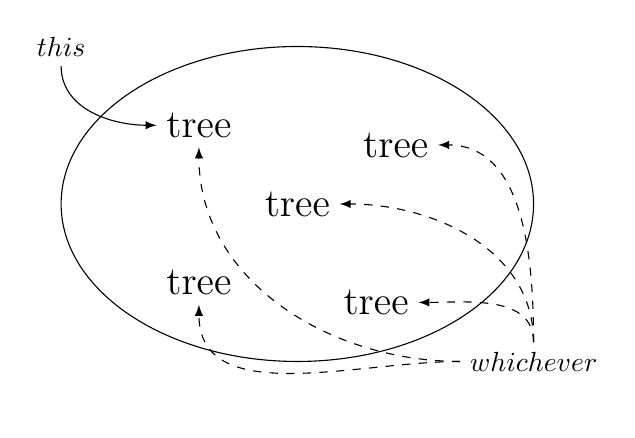
\begin{tikzpicture}
		\node (ellipse)	at (3,2)	{};
		\node (this)	at (0,4)	{$this$};
		\node (some)	at (6,0)	{$whichever$};

		\node (fig_1)	at (2-0.25 , 3+0.00)	{\Large\faicon{tree}};
		\node (fig_2)	at (4+0.25 , 3-0.25)	{\Large\faicon{tree}};
		\node (fig_3)	at (2-0.25 , 1+0.00)	{\Large\faicon{tree}};
		\node (fig_4)	at (4+0.00 , 1-0.25)	{\Large\faicon{tree}};
		\node (fig_5)	at (3-0.00 , 2+0.00)	{\Large\faicon{tree}};

		\draw (ellipse) ellipse [x radius=3, y radius=2];

		\draw[-latex] (this) to [out=south, in=west] (fig_1);
		\draw[-latex, dashed] (some) to [out=west, in=south] (fig_1);
		\draw[-latex, dashed] (some) to [out=north, in=east] (fig_2);
		\draw[-latex, dashed] (some) to [out=west, in=south] (fig_3);
		\draw[-latex, dashed] (some) to [out=north, in=east] (fig_4);
		\draw[-latex, dashed] (some) to [out=north, in=east] (fig_5);
	\end{tikzpicture}
	}
\xe
\end{figure}

\begin{morphlex}
\ex\label{ex:memorphlex}%
\adjustbox{valign=t}{%
	\begin{tabu} {\usetabu{morphlexnarrow}}
	\rayr{\larger me/}{mə-}
		& Cl
		& \begin{tabular}[t]{l l l}
			\ups{\Def} & = & $-$ \\
			\ups{specific} & = & $-$ \\
		\end{tabular}
	\end{tabu}%
}
\xe
\end{morphlex}

Since according to \citet[152]{lyons1999}, demonstratives are inherently
definite---and their reference is specific, too---the deictic proclitics
\xayr{Ed/}{eda-}{this}, \xayr{Ad/}{ada-}{that}, and \xayr{d/}{da-}{such} are in
complementary distribution with the inspecificity marker, as demonstrated by
(\ref{ex:inspecdeix}): neither combination of \rayr{me/}{mə-} and \rayr{Ed/}
{eda-} in (\ref{ex:inspecdeix}cd) results in an ungrammatical sentence because 
\rayr{Ed/}{eda-} encodes [\Def{}~$+$, \textsc{specific}~$+$] while \rayr{me/}
{mə-} encodes [\Def{}~$-$, \textsc{specific} $-$]. Attempting to assign
opposing values to the same feature (\Def{} and \textsc{specific},
respectively) must fail, since these cannot be united at the functional level.

\pex\label{ex:inspecdeix}
\a\label{ex:inspecdeix_1}\begingl
	\gla Ang nakasyon nihanye eda-mehirya. //
	\glb ang nakas-yon nihan-ye-Ø eda=mehir-ya //
	\glc \AgtT{} grow-\TplN{} fruit-\Pl{}-\Top{} this=tree-\Loc{} //
	\glft `Fruits are growing on this tree.' //
\endgl

\a\label{ex:inspecdeix_2}\begingl
	\gla Ang nakasyon nihanye mə-mehirya. //
	\glb ang nakas-yon nihan-ye-Ø mə=mehir-ya //
	\glc \AgtT{} grow-\TplN{} fruit-\Pl{}-\Top{} whichever=tree-\Loc{} //
	\glft `Fruits are growing on whichever tree.' //
\endgl

\a\ljudge*\label{ex:inspecdeix_3}\begingl
	\gla Ang nakasyon nihanye mə-eda-mehirya. //
	\glb ang nakas-yon nihan-ye-Ø mə=eda=mehir-ya //
	\glc \AgtT{} grow-\TplN{} fruit-\Pl{}-\Top{} whichever=this=tree-\Loc{} //
\endgl

\a\ljudge*\label{ex:inspecdeix_4}\begingl
	\gla Ang nakasyon nihanye eda-mə-mehirya. //
	\glb ang nakas-yon nihan-ye-Ø eda=mə=mehir-ya //
	\glc \AgtT{} grow-\TplN{} fruit-\Pl{}-\Top{} this=whichever=tree-\Loc{} //
\endgl

\xe

The inspecificity proclitic \rayr{me/}{mə-} cannot commonly be combined with
pronouns, since personal pronouns as well as demonstrative pronouns have a
definite reference; combining the clitic with an indefinite pronoun would be
redundant. With interrogative pronouns it is feasible to use \rayr{me/}{mə-} as
an intensifier, though without the vulgar tone of the English translation given
in the following example:

\ex\label{ex:meinter}\begingl
	\gla Amangreng mə-simin? //
	\glb amang=reng mə=simin //
	\glc happen=\TsgI{}.\Aarg{} whichever=how //
	\glft `How the fuck did that happen?' //
\endgl\xe

\subsubsection{Quantifying clitics}

As described in \autoref{clitics_quant} (p.~\pageref{clitics_quant}~ff.) and 
\autoref{subsec:quantifiers}, Ayeri has a number of suffixed---that is,
enclitic---quantifiers which can attach to inflected nouns. These, along with
their non-clitic counterparts, are modifiers and are thus part of an NP's list
of adjuncts, \Adjc{}, along with adjectives and nominal adjuncts. An example of
this is given in (\ref{ex:nounquantavm}), using the clitic quantifier
\xayr{/iknF}{-ikan}{much, many; very}. Since the quantifier already lexically
expresses a multitude in this case, the noun does not carry redundant plural
marking.

\pex\label{ex:nounquantavm}
\a\label{ex:nounquantavm_1}\begingl
	\gla Sa tahayeng bisuay-ikan ban //
	\glb sa taha=yeng bisuay.Ø=ikan ban //
	\glc \PatT{} have=\TsgF{}.\Aarg{} idea.\Top{}=many good //
	\glft `She has many good ideas.' //
\endgl

\a\label{ex:nounquantavm_2}
\begin{avm}
\[
%	\Pred	&	\astruct{have}{\ups{\Subj}, \ups{\Obj}} \\
	\Top	&	\[
					\Pred	&	`idea' \\
					\Anim	&	$+$ \\
					\Case	&	\Parg \\
					\Adjc	&	\{
									\[
										\Pred	&	`many' \\
									\], \\
									\[
										\Pred	&	`good' \\
									\]
								\}
				\] \tikzmark{nounquantavm_top} \\

	% \Subj	&	\[
	% 				\Pred	&	`pro' \\
	% 				\Anim	&	$+$ \\
	% 				\Case	&	\Aarg \\
	% 				\Gend	&	\F \\
	% 				\Num	&	\Sg \\
	% 				\Pers	&	\Third \\
	% 			\] \\

	\Obj	&	\tikzmark{nounquantavm_obj} \\
\]
\end{avm}

\begin{tikzpicture}[remember picture, overlay]
\draw [rounded corners=1ex] ([yshift=1ex]{pic cs:nounquantavm_top})
	-- ++(east:1em) |- ([yshift=1ex]{pic cs:nounquantavm_obj}););
\end{tikzpicture}

\xe

Clitic quantifiers as well can combine at least with independent personal
pronouns especially in the plural, and demonstrative pronouns. A clitic
quantifier can also still be recognized in the interrogative pronoun 
\xayr{siknF}{sikan}{how many}, although here it is incorporated into the
pronoun itself, that is, there is no productive combination of interrogative
pronouns and quantifiers, with the exception of \xayr{sinY}{sinya}{who}. With
indefinite pronouns, quantifiers are somewhat redundant in some combinations,
though it is feasible in this regard to use them for emphasis. The relativizer
\rayr{si}{si} and its declined forms cannot be quantified; the simple and most
common form of the relativizer, \rayr{si}{si}, is also unstressed, which makes
it a bad host for a clitic. Combinations of pronouns and quantifying clitics
are illustrated in (\ref{ex:proquant}).

\pex\label{ex:proquant}
\a\label{ex:proquant_perspro}\begingl
	\gla Ang koronay tas-ikan. //
	\glb ang koron=ay.Ø tas=ikan //
	\glc \AgtT{} know=\Fsg{}.\Top{} \TplM{}.\Parg{}=many //
	\glft `I know many of them.' //
\endgl

\a\label{ex:proquant_dempro}\begingl
	\gla Kalam adanyana-ikoy //
	\glb kalam adanya-na=ikoy //
	\glc true that.one-\Gen{}=not.much //
	\glft `Little about that is true.' //
\endgl

\a\label{ex:proquant_interpro}\begingl
	\gla Yomāra sinyareng-ma? //
	\glb yoma-ara sinya-reng=ma //
	\glc exist-\TsgI{} what-\AargI{}=enough //
	\glft `What is there enough of?' //
\endgl

\a\label{ex:proquant_indefpro_1}\begingl
	\gla Ang ilye {} @ Pada enyaley-kay cam. //
	\glb ang il-ye Ø= Pada enya-ley=kay cam //
	\glc \Aarg{} give-\TsgF{} \Top{}= Pada everything-\PargI{}=a.little 
		\TplM{}.\Dat{} //
	\glft `Pada gave them a little of everything.' //
\endgl

\a\label{ex:proquant_indefpro_2}\begingl
	\gla Enyāng-hen siyan? //
	\glb enya-ang=hen siyan //
	\glc everyone-\Aarg{}=all where //
	\glft \textit{Literally:} `Where is all of everyone?' //
\endgl

\a\label{ex:proquant_relpro}\ljudge*\begingl
	\gla Le inttang piyu si-ma ya yomareng bukuno. //
	\glb le int=tang piyu-Ø si=ma ya yoma-reng bukuno-Ø //
	\glc \PargI{} buy=\TplM{}.\Aarg{} grain-\Top{} \Rel{}=enough \LocT{}
	exist=\TsgI{}.\Aarg{} storage-\Top{} //
	\glft \textit{Intended:} `They are buying the grain enough of which is 
		in the storage' //
\endgl

\xe

\section{Adjective and adverb phrases}
\label{sec:adjps-advps}

Adjectives and adverbs in Ayeri are largely similar in that they can both be
modified by adverbs like \fw{very}, and they both modify heads: adjectives
modify nouns, adverbs modify everything else. \citet[51]{carnie2013} urges his
readers to think about whether it is sensible to distinguish between the two
categories, so let us focus in this section on structural similarities and
dissimilarities between the two, as well as their distribution as morphemes.

\subsection{Adjective phrases}
\label{subsec:adjps}

As described in the previous section, APs are usually found as adjuncts of NPs
or DPs, where they describe properties of these nominal elements. Adjectives
are likewise commonly found as \Plink{} in copula clauses, which will be dealt
with in \autoref{subsec:eqs}. Possessive pronouns can be used as adjective-like
modifiers as well, though they are probably still better classified as DP
heads, since they are functional morphemes. Possessive adjectives thus also do
not share all the morphological properties of adjectives, for instance, they
cannot be compared (see \autoref{phsec:possadj}, p.~\pageref{phsec:possadj}),
also they can only be instanced once. In other words, it is not possible to
modify the same noun with multiple possessive morphemes, which means that they
are not part of \Adjc{}. The phrase-structure rule in (\ref{ex:adjpstruct}) and
the c-structure tree in (\ref{ex:adjpcstruct}) show how an AP is constructed.

\begin{figure}
\pex\label{ex:adjpstruct}
\a AP → \anno*{\xhead{A}} $\left(\anno*[{\pass{\GF}}]{XP}\right)$
\xe

\ex~\label{ex:adjpcstruct}\labels
\begin{forest}
[{\anno[\{\elem{\Adjc} | \pass{\Plink}\}]{AP}}
%	[\anno{\xbar{A}}
		[\anno{\xhead{A}}]
		[{$\left(\anno[{%
				\pass{\GF}%
			}]{XP}\right)$%
		}]
%	]
]
\end{forest}
\xe
\end{figure}

Adjective phrases have an adjective as their lexical head. This head may be
extended by modifiers adjoined to \xbar{A}; \xbar{A} repeats for the adjunction
of multiple modifiers. Since modifiers follow their heads here as well, APs are
also a right-branching constituent. Modifiers of adjectives are subsumed under
the label XP here, which here stands for AdvP, NP, DP, and CP. An example of
each phrase type modifying an adjective is given in (\ref{ex:adjmod}) and 
(\ref{ex:adjmod2}).

\begin{figure}
\pex\label{ex:adjmod}
\a\label{ex:adjmod_adv}%
	\begin{minipage}[t]{.667\remaining}%
	\begingl
		\glpreamble adjective + AdvP adjunct: //
		\gla Adareng bisuayas sadayo kalam. //
		\glb ada-reng bisuay-as sadayo kalam //
		\glc that-\AargI{} idea-\Parg{} crazy truly //
		\glft `That is a truly crazy idea.' //
	\endgl~\\

	\begin{avm}
	\[
		\Obj	&	\[
			\Pred	&	`idea' \\
			\Anim	&	$+$ \\
			\Case	&	\Parg \\
			\Adjc	&	\{\[
				\Pred	&	`crazy` \\
				\Adjc	&	\{\[
					\Pred	&	`truly' \\
				\]\} \\
			\]\} \\
		\]
	\]
	\end{avm}
	\end{minipage}
	~
	\begin{forest} narrower nodes, shorter edges, italic leaves,
	[{\anno[\pass{\Obj}]{NP}}
%		[\anno{\xbar{N}}
			[\anno{\xhead{N}}
				[bisuayas]
			]
			[{\anno[\elem{\Adjc}]{AP}}
%				[\anno{\xbar{A}}
					[\anno{\xhead{A}}
						[sadayo]
					]
					[{\anno[\elem{\Adjc}]{AdvP}}
						[{kalam}, roof]
					]
%				]
			]
%		]
	]
	\end{forest}\medskip

\a\label{ex:adjmod_np}%
	\begin{minipage}[t]{.667\remaining}
	\begingl
		\glpreamble adjective + NP complement: //
		\gla Yang mino yanena nā. //
		\glb yang mino yan-ena nā //
		\glc \Fsg{}.\Aarg{} happy son-\Gen{} \Fsg{}.\Gen{} //
		\glft `I am happy about my son.' //
	\endgl~\\

	\begin{avm}
	\[
		\Plink	&	\[
			\Pred		&	\astruct{happy}{\Oblq{src}} \\
			\Oblq{src}	&	\[
				\Pred	&	`son' \\
				\Case	&	\Gen \\
				\Poss	&	\[
					% \Pred	&	`$pro$' \\
					% \Case	&	\Gen \\
					% \Num	&	\Sg \\
					% \Pers	&	\First \\
					\avmspan{``my''} \\
				\] \\
			\] \\
		\] \\
	\]
	\end{avm}
	\end{minipage}
	~
	\begin{forest} narrower nodes, shorter edges, italic leaves,
	[{\anno[\pass{\Plink}]{AP}}
%		[\anno{\xbar{A}}
			[\anno{\xhead{A}}
				[mino]
			]
			[{\anno[\pass{\Oblq{src}}]{NP}}
				[{yanena nā}, roof]
			]
%		]
	]
	\end{forest}
\xe
\end{figure}

\begin{figure}
\pex\label{ex:adjmod2}
\a\label{ex:adjmod_dp}%
	\begin{minipage}[t]{.667\remaining}
	\begingl
		\glpreamble adjective + DP complement: //
		\gla Yang mino yayam. //
		\glb yang mino yayam //
		\glc \Fsg{}.\Aarg{} happy \TsgM{}.\Dat{} //
		\glft `I am happy for him.' //
	\endgl~\\

	\begin{avm}
	\[
		\Plink	&	\[
			\Pred	&	\astruct{happy}{\ups{\Oblq{goal}}} \\
			\Oblq{goal}	&	\[
				% \Pred	&	`$pro$' \\
				% \Case	&	\Dat \\
				% \Num	&	\Sg \\
				% \Pers	&	\Second \\
				\avmspan{``him''} \\
			\] \\
		\] \\
	\]
	\end{avm}
	\end{minipage}
	~
	\begin{forest} narrower nodes, shorter edges, italic leaves,
	[{\anno[\pass{\Plink}]{AP}}
%		[\anno{\xbar{A}}
			[\anno{\xhead{A}}
				[mino]
			]
			[{\anno[\pass{\Oblq{goal}}]{DP}}
				[{yayam}, roof]
			]
%		]
	]
	\end{forest}\medskip

\a\label{ex:adjmod_cp}%
	\begin{minipage}[t]{.667\remaining}
	\begingl
		\glpreamble adjective + CP complement: //
		\gla Yang valuy yomavāng edaya. //
		\glb yang valuy yoma=vāng edaya //
		\glc \Fsg{}.\Aarg{} glad exist=\Second.\Aarg{} here //
		\glft `I am glad you are here.' //
	\endgl~\\

	\begin{avm}
	\[
		\Plink	&	\[
			\Pred	&	\astruct{glad}{\ups{\Compl}} \\
			\Compl	&	\[
				\Pred		&	\astruct{exist}{...} \\
				\Subj		&	\[...\] \\
				\Oblq{loc}	&	\[...\] \\
			\] \\
		\] \\
	\]
	\end{avm}
	\end{minipage}
	~
	\begin{forest} narrower nodes, shorter edges, italic leaves,
	[{\anno[\pass{\Plink}]{AP}}
%		[\anno{\xbar{A}}
			[\anno{\xhead{A}}
				[valuy]
			]
			[{\anno[\pass{\Compl}]{CP}}
				[{yomavāng\\ edaya}, roof]
			]
%		]
	]
	\end{forest}\medskip

\xe
\end{figure}

Example (\ref{ex:adjmod_adv}) gives the f- and c-structures for the adjective
phrase to show that \Adjc{} may be recursive: an adjective which serves as one
of many modifiers to a noun can itself be modified by adverbs. Likewise, an
adjective--adverb combination can be complemented by an NP, as shown in
(\ref{ex:adjmod_dp}). Especially in (\ref{ex:adjmod_np}) and
(\ref{ex:adjmod_dp}) we can see Ayeri's propensity for using cases with
complements where English would use prepositions. Thus, in
(\ref{ex:adjmod_np}), `about' is expressed by putting the nominal complement in
the genitive case: the NP complement expresses the source by which the
experiencing subject becomes happy. This, however, should not be conflated with
a possessor, \Possr{}, but should be labeled separately as an oblique
complement, \Oblq{src}. Similarly, the recipient of the subject's happiness
appears as an NP complement in the (ethical) dative in (\ref{ex:adjmod_dp}).
Instrumental and causative NP complements instead of PPs may be found as well.

Since in \Lfg{}, empty \xbar{X} nodes are collapsed, \Lfg{}'s version of X-bar
theory does not strictly distinguish between complements and adjuncts
\citep[127, footnote 52]{bresnan2016}; the functional annotation provides
information about whether a sister node to \xhead{X} is a complement or an
adjunct instead. How do we know that the extensions to the adjective in
(\ref{ex:adjmod}) are complements rather than adjuncts? X-bar theory posits
that complements and adjuncts are on different \xbar{X} branches---a complement
is a sister to the head whereas an adjunct is its cousin, so to speak, compare 
(\ref{ex:xbartree}).

\begin{figure}
\ex\label{ex:xbartree}
\begin{forest}
[XP, for tree={s sep=2em}%, l sep=2em}
	[\xbar{X}
		[\xbar{X}
			[\xhead{X}, name=head]
			[ZP, name=complement]
		]
		[YP, name=adjunct]
	]
	[WP, name=spec]
]
%
\node [right=1em of spec, font=\itshape]
	(spec_label) {specifier};
\draw [-latex] (spec_label) -- (spec);
%
\node [right=1em of complement, font=\itshape]
	(complement_label) {complement};
\draw [-latex] (complement_label) -- (complement);
%
\node [right=1em of adjunct, font=\itshape]
	(adjunct_label) {adjunct};
\draw [-latex] (adjunct_label) -- (adjunct);
%
\node [left=1em of head, font=\itshape]
	(head_label) {head};
\draw [-latex] (head_label) -- (head);
\end{forest}
\xe
\end{figure}

How does this hypothesis fare when applying constituency tests, though? With
regards to complements and adjuncts to NP, \citet{carnie2013} explains,
\textcquote[182]{carnie2013}{Since complements are sisters to X and not Xʹ,
they cannot stand next to the word \fw{one}. Adjuncts, by definition, can}. To
target \xbar{A} nodes, we need something corresponding to English \fw{so},
which we find in Ayeri \xayr{d/}{da-}{thus, so, such}. Since adverbs are
adjuncts, it is possible to replace the adjective \xayr{sdyo}{sadayo}{crazy} in
(\ref{ex:soreplacement}a) with \rayr{d/}{da-} in (\ref{ex:soreplacement}b); the
\xbar{A} in (\ref{ex:soreplacement}a) being targeted is the sister to AdvP.

\begin{figure}
\ex\label{ex:soreplacement}\labels%
\begin{minipage}[t]{0.5\remaining}%
\tl\quad\begingl%
	\gla bisuayas sadayo kalam //
	\glb bisuay-as sadayo kalam //
	\glc idea-\Parg{} crazy truly //
	\glft `a truly crazy idea' //
\endgl\\[1ex]

\tl\quad\begingl
	\gla Da-kalam bisuayang. //
	\glb da=kalam bisuay-ang //
	\glc so=truly idea-\Aarg{} //
	\glft `The idea is truly so.' //
\endgl
\end{minipage}
~
\begin{forest} shorter edges, italic leaves,
% Superfluous bar levels here are on purpose!
[NP
	[\xbar{N}
		[\xbar{N}
			[\xhead{N}
				[bisuayas]
			]
		]
		[AP
			[\xbar{A}
				[\xbar{A}, draw, circle
					[\xhead{A}
						[sadayo]
					]
				]
				[AdvP
					% [\xbar{Adv}
					% 	[\xbar{Adv}
					% 		[\xhead{Adv}
								[kalam, roof]
					% 		]
					% 	]
					% ]
				]
			]
		]
	]
]
\end{forest}
\xe
\end{figure}

Continuing this replacement test for the other example sentences from
(\ref{ex:adjmod}), we can see that the outcomes are ungrammatical; the NPs are
dependent on their lexical head, which cannot be omitted or replaced by a
pro-form. The idiomatic English translations in (\ref{ex:soreplacement_2})
somewhat conceal this.\footnote{At least to me, as a non-native speaker of
English, these translations do not sound too odd if context is taken into
consideration. \citet[181]{carnie2013} gives an example *\fw{the one of poems
with a red cover}, referring to a book. His point is that \fw{of poems} is a
complement of \fw{the book}, so \fw{the book} cannot be replaced by a pro-form
like \fw{one}. However, he notes that at least some native English speakers
find this example acceptable. Personally, I do not take offense either, but I
am not a native speaker.} The literal translations try to show that the
complements are more tightly integrated into the sentence in Ayeri than in the
idiomatic translations in an attempt to convey how they must seem non-sensical
to an Ayeri speaker.

\begin{figure}
\pex\label{ex:soreplacement_2}
\a\label{ex:soreplacement_2_1}\ljudge*\begingl
	\gla Yang da-yanena nā. //
	\glb yang da=yan-ena nā //
	\glc \Fsg{}.\Aarg{} so=son-\Gen{} \Fsg{}.\Gen{} //
	\glft `I am so about my son.'\\
		\textit{Literally:} `I am my son's so.' //
\endgl
\a\label{ex:soreplacement_2_2}\ljudge*\begingl
	\gla Yang da-yayam. //
	\glb yang da=yayam //
	\glc \Fsg{}.\Aarg{} so=\TsgM{}.\Dat{} //
	\glft `I am so for him.' \\
		\textit{Literally:} `I am him so.' //
\endgl

\a\label{ex:soreplacement_2_3}\ljudge*\begingl
	\gla Yang da-yomavāng edaya. //
	\glb Yang da=yoma=vāng edaya //
	\glc \Fsg{}.\Aarg{} so=exist=\Second{}.\Aarg{} here //
	\glft `I am so that you are here.' //
\endgl
\xe
\end{figure}

% FIXME: Can this be mitigated by replacing "da-" with a full demonstrative?
% Would the conjunct be interpreted as an adjunct in this case? Why?

Further complications arise with regards to complementation in that non-clitic
quantifiers like \xayr{AMkYu}{ankyu}{really} usurp the complement position so
that an adjective's complement XP appears as an adjunct. This is possibly due
to syntactic weight \citep{wechsler2009}. Example (\ref{ex:intrusivequant})
attempts to illustrate the c-structure for a displaced CP; the arrow shows the
apparent movement from complement to adjunct.

\begin{figure}
\ex\label{ex:intrusivequant}%
\begingl[aboveglbskip=1em]
	\gla Yang valuy {\_\tikzmark{intrusivequant2_1}} ankyu, 
	{$[$yomavāng edaya\tikzmark{intrusivequant2_2}$]$}. //
	\glb yang valuy {} ankyu yoma=vāng edaya //
	\glc \Fsg{}.\Aarg{} glad {} really exist=\Second{}.\Aarg{} here //
	\glft `I am really glad you are here.' //
\endgl
\begin{tikzpicture}[remember picture, overlay]
\draw [-latex] ([xshift=-.25em,yshift=-.75ex]{pic cs:intrusivequant2_1}) 
|- ++ (south:.75em) -| ([xshift=-.5*width("yomavāng edaya"),yshift=-.75ex]{pic
cs:intrusivequant2_2});
\end{tikzpicture}

\begin{forest} shorter edges, italic leaves,
[{\anno[\pass{\Plink}]{AP}}
%	[\anno{\xbar{A}}
		[\anno{\xbar{A}}
			[\anno{\xbar{A}}
				[\anno{\xhead{A}}
					[valuy]
				]
				[$\epsilon$, name=CP_orig]
			]
			[{\anno[\elem{\Adjc}]{AdvP}}
				[ankyu, roof]
			]
		]
		[{\anno[\pass{\Compl}]{CP}}
			[{yomavāng edaya}, roof, name=CP]
		]
%	]
]
%
\draw [-latex, dashed] (CP_orig) to [out=south, in=south, "?" {midway, below}] 
(CP);
\end{forest}
\xe
\end{figure}

In \Lfg{}, however, there are no transformations by design; instead,
c-structure is taken to be base-generated while acknowledging that different
languages may have different phrase-structure plans, and the functional
structure is what creates a sense of cohesion. Thus, even though the CP
in (\ref{ex:intrusivequant}) appears dislocated, the information is still found
in the `right' place in f-structure independent of the diverging c-structure,
compare the \Avm{} in (\ref{ex:intrusivequant_fstruct}), where the adjective
is given as having an oblique nominal complement, and what surfaces as the CP
adjunct is annotated accordingly as \Compl{}, not as \Adjc{}, even though in
c-structure it appears in the position of an adjunct.
% FIXME: Gahd, I *hope* this paragraph makes sense ...

\begin{figure}
\ex\label{ex:intrusivequant_fstruct}
\begin{avm}
\[
	\Plink	&	\[
		\Pred	&	\astruct{glad}{\ups{\Compl}} \\
		\Adjc	&	\[
			\Pred	&	`really' \\
		\]\\
		\Compl	&	\[
			\Pred	&	\astruct{exist}{\ups{\Subj}, \ups{\Oblq{loc}}} \\
			\Subj	&	\[
				\Pred	&	`$pro$' \\
				\Case	&	\Aarg \\
				\Pers	&	\Second \\
			\] \\

			\Oblq{loc}	&	\[
				\Pred	&	`here' \\
			\] \\
		\] \\
	\] \\
\]
\end{avm}
\xe
\end{figure}

As pointed out in \autoref{sec:adjectives}, Ayeri's adjectives inflect very
little, since there is no agreement morphology. However, it is possible for
adjectives to be compared and to be negated by means of morphology. This is
reflected in the functional annotations given in (\ref{ex:adjmorphlex}). The
features \Compar{} and \Neg{} appear in brackets here, since they do not
apply to every adjective: adjectives normally appear in the positive in both
regards, comparison and polarity, and are morphologically unmarked in these
cases.

\begin{morphlex}
\ex\label{ex:adjmorphlex}%
\adjustbox{valign=t}{%
	\begin{tabu} {\usetabu{morphlexnarrow}}
	...
		& A
		& \begin{tabular}[t]{l l l}
			\ups{\Pred} & = & `...' \\
			(\ups{\Compar} & = & \{\Comp, \Supl\}) \\
			(\ups{\Neg} & = & $+$) \\
		\end{tabular}
	\end{tabu}%
}
\xe
\end{morphlex}

Examples of the different ways an adjective may be morphologically marked and
their respective representation as an \Avm{} are given in (\ref{ex:adjmorph}).

\pex\label{ex:adjmorph}
\a\label{ex:adjmorph_compar}
\begin{minipage}[t]{.5\remaining}
\begingl
	\gla nake-vā //
	\glb nake=vā //
	\glc tall=\Supl{} //
	\glft `tallest' //
\endgl
\end{minipage}
~
\begin{avm}
\[
	\Pred	&	`tall' \\
	\Compar	&	\Supl \\
\]
\end{avm}

\a\label{ex:adjmorph_neg}
\begin{minipage}[t]{.5\remaining}
\begingl
	\gla mingoy //
	\glb ming-oy //
	\glc capable-\Neg{} //
	\glft `incapable' //
\endgl
\end{minipage}
~
\begin{avm}
\[
	\Pred	&	`capable' \\
	\Neg	&	$+$ \\
\]
\end{avm}

\a\label{ex:adjmorph_compar+neg}
\begin{minipage}[t]{.5\remaining}
\begingl
	\gla pasīsoy-eng //
	\glb pasīsa-oy=eng //
	\glc interesting-\Neg{}=\Comp{} //
	\glft `more uninteresting' //
\endgl
\end{minipage}
~
\begin{avm}
\[
	\Pred	&	`interesting' \\
	\Compar	&	\Comp \\
	\Neg	&	$+$ \\
\]
\end{avm}

\xe

As described before (\autoref{subsec:adjcomp}), the morphemes used for
synthetic comparison of adjectives are grammaticalized clitics literally
meaning `rather, more' (\rayr{/ENF}{-eng}) and `most' (\rayr{/vaa}{-vā}) as
lexical quantifiers. With adjectives, there is no clear-cut line between their
functional and their lexical use. I have analyzed them here as functional,
since they may be interpreted as such, depending on context. As we have
observed before (\autoref{subsec:quantifiers}), quantifier clitics may modify
adjectives like any other adverbial modifiers, except that their surface form
is clitic rather than free. Quantifying adverbs, both enclitic and free, thus
also find themselves in \Adjc{}.

\pex\label{ex:adjquant3}
\a
\begin{minipage}[t]{.5\remaining}
\begingl
	\gla luyu-mas //
	\glb luyu=mas //
	\glc strange=kind.of //
	\glft `kind of strange' //
\endgl
\end{minipage}
~
\begin{avm}
\[
	\Pred	&	`strange' \\
	\Adjc	&	\{\[
					\Pred	&	`kind of' \\
				\]\} \\
\]
\end{avm}

\a\label{ex:adjadvconv}
\begin{minipage}[t]{.5\remaining}
\begingl
	\gla valuy ipan. //
	\glb valuy ipan //
	\glc glad extremely //
	\glft `extremely glad' //
\endgl
\end{minipage}
~
\begin{avm}
\[
	\Pred	&	`glad' \\
	\Adjc	&	\{\[
					\Pred	&	`extremely' \\
				\]\} \\
\]
\end{avm}

\xe

\subsection{Adverb phrases}
\label{subsec:advps}

Adverbs, as (\ref{ex:adjadvconv}) shows, can easily be converted from
adjectives. Thus, \xayr{IpnF}{ipan}{extreme}, which is normally an adjective,
is used there in an adverbial way, meaning `extremely'. The word stays the
same, however: \rayr{IpnF}{ipan}, without a derivative affix akin to English
\fw{-ly} or French \fw{-ment}. Since adverbs and adjectives are largely similar
in that they provide additional information about the nature or circumstance of
a noun or another part of speech, \citet{carnie2013} poses the question whether
adjectives and adverbs should be better analyzed as being part of the same
category. He reasons that

\blockcquote[51]{carnie2013}{Both Adj and Adv can be modified by the word
\fw{very}, and they both have the same basic function in the grammar---to
attribute properties to the items they modify. In fact, the only major
distinction between them is syntactic: Adjectives appear inside NPs, while
adverbs appear elsewhere.}

Adjectives and adverbs are in complementary distribution, which, he writes,
would normally be taken as evidence that these two things are of the same
category. In fact, the only reason \citet{carnie2013} adduces for keeping the
two categories apart is \textquote{because they are familiar to most people},
and he prompts the reader to consider that uniting them in a single
supercategory \textcquote[51]{carnie2013}{might provide a better analysis and
might be better motivated scientifically}. \citet[126]{bresnan2016} also
classify both adjectives and adverbs as heads of AP with reference to
\citet{emonds1976}. As described in \autoref{sec:adverbs}, the only morphology
attributive adverbs take in Ayeri is comparison morphology and negation. This
is the same as with adjectives indeed, hence the functional specifications
appear equal:

\begin{morphlex}
\ex\label{ex:advmorphlex}%
\adjustbox{valign=t}{%
	\begin{tabu} {\usetabu{morphlexnarrow}}
	...
		& A
		& \begin{tabular}[t]{l l l}
			\ups{\Pred} & = & `...' \\
			(\ups{\Compar} & = & \{\Comp, \Supl\}) \\
			(\ups{\Neg} & = & $+$) \\
		\end{tabular}
	\end{tabu}%
}
\xe
\end{morphlex}

If we look at the phrase structure (\ref{ex:advpstruct}) and the c-structure
(\ref{ex:advpcstruct}) for adverbs, however, there is a slight difference in
that adverbs cannot serve as \XCompl{} in equative statements; they also can
only be modified by other adverbs, but not by  NP, DP, or CP.\footnote{For
adjectives, compare (\ref{ex:adjpstruct}), (\ref{ex:adjpcstruct}), and
(\ref{ex:adjmorphlex}) in \autoref{subsec:adjps}.} On the other hand,
adjectives are restricted to nominal contexts whereas adverbs may modify any
other lexical category: verbs, adjectives, prepositions, as well as other
adverbs.

\begin{figure}
\pex\label{ex:advpstruct}
\a AdvP → \anno*{\xhead{Adv}} $\left(\anno*[{\elem{\Adjc}}]{AdvP}\right)$
\xe

\ex~\label{ex:advpcstruct}\labels
\begin{forest}
[{\anno[\elem{\Adjc}]{AdvP}}
%	[\anno{\xbar{Adv}}
		[\anno{\xhead{Adv}}]
		[{$\left(\anno[{%
				\elem{\Adjc}%
			}]{AdvP}\right)$%
		}]
%	]
]
\end{forest}
\xe
\end{figure}

Example (\ref{ex:advmod}) gives examples of modifiers of adverbs. These
modifiers are often quantifying adverbs, whether clitic ones or free ones. 
Since adjectives and adverbs are not distinguished by morphology, 
the heads of both phrases, \xayr{vkis}{vakisa}{careful} and \xayr{bit}{bita}
{ordinary, normal}, may be interpreted as well as adjectives, depending on
context.

\begin{figure}
\pex\label{ex:advmod}
\a\label{ex:advmod_free}%
\begin{minipage}[t]{.667\remaining}%
\begingl
	\gla bita ikan-ikan //
	\glb bita ikan.ikan //
	\glc ordinarily completely //
	\glft `completely ordinarily' //
\endgl~\\

\begin{avm}
\[
	\Adjc	&	\{\[
		\Pred	&	`ordinarily' \\
		\Adjc	&	\{\[
			\Pred	&	`completely' \\
		\]\} \\
	\]\} \\
\]
\end{avm}
\end{minipage}
~
\begin{forest} shorter edges, italic leaves,
[{\anno[\elem{\Adjc}]{AdvP}}
%	[\anno{\xbar{Adv}}
		[\anno{\xhead{Adv}}
			[bita]
		]
		[{\anno[\elem{\Adjc}]{AdvP}}
%			[\anno{\xbar{Adv}}
				[\anno{\xhead{Adv}}
					[ikan-ikan]
				]
%			]
		]
%	]
]
\end{forest}

\a\label{ex:advmod_clitic}%
\begin{minipage}[t]{.667\remaining}%
\begingl
	\gla vakisoy @ -ma //
	\glb vakisa-oy =ma //
	\glc carefully-\Neg{} =enough //
	\glft `not carefully enough' //
\endgl~\\

\begin{avm}
\[
	\Adjc	&	\{\[
		\Pred	&	`carefully' \\
		\Neg	&	$+$ \\
		\Adjc	&	\{\[
			\Pred	&	`enough' \\
		\]\} \\
	\]\} \\
\]
\end{avm}
\end{minipage}
~
\begin{forest} shorter edges, italic leaves,
[{\anno[\elem{\Adjc}]{AdvP}}
%	[\anno{\xbar{Adv}}
		[\anno{\xhead{Adv}}
			[\anno{\xhead{Adv}}
				[vakisoy]
			]
			[{\anno[\elem{\Adjc}]{Cl}}
				[-ma]
			]
		]
%	]
]
\end{forest}
\xe
\end{figure}

For the clitic \xayr{ku}{ku}{like} described above (\ref{ex:postkumorphlex}),
it was necessary to make a separate rule for the prefixed and suffixed version.
This, however, is not necessary for clitic quantifiers, since they attach
immediately to the head they modify rather than to the last word of the AdvP.
Besides their diverging morphological distribution, it may thus be assumed that
the functional scheme given in (\ref{ex:advmorphlex}) also holds for enclitic
quantifiers. Quantifiers appear to be able to be modified in turn, as
illustrated by (\ref{ex:clitics_55}) from \autoref{clitics_quant} (compare
p.~\pageref{ex:clitics_55}), which is repeated again here, abbreviated; 
\xayr{/IknF}{ikan}{much, many, very} is modified in this case by \xayr{kgnF}
{kagan}{far too} to convey the meaning `far too many'.
% FIXME: % CAN YOU EVEN HAVE A HIERARCHICAL STRUCTURE OF MODIFICATION AMONG
% CLITICS, LIKE ONE CLITIC MODIFYING ANOTHER?

\ex\label{ex:clitics_55_short}%
%\begin{minipage}[t]{.667\remaining}%
\begingl
	\gla keynam @ -ikan kagan //
	\glb keynam-Ø =ikan kagan //
	\glc people-\Top{} =many far.too //
	\glft `far too many people' //
\endgl~\\

% \begin{avm}
% \[
% 	\Top	&	\[
% 					\Pred	&	`people' \\
% 					\Anim	&	$+$ \\
% 					\Case	&	\Aarg{} \\
% 					\Num	&	\Pl \\
% 					\Pers	&	\Third \\

% 					\Adjc	&	\{\[
% 									\Pred	&	`many' \\
% 									\Adjc	&	\[
% 										\Pred	&	`far too' \\
% 									\] \\
% 								\]\} \\
% 				\] \tikzmark{clitics_55_short_Top} \\

% 	\Subj	&	~\tikzmark{clitics_55_short_subj} \\
% \]
% \end{avm}
% \begin{tikzpicture}[remember picture, overlay]
% \draw [rounded corners=1ex] ([yshift=1ex]{pic cs:clitics_55_short_Top})
% 	-- ++(east:1em) |- ([yshift=1ex]{pic cs:clitics_55_short_subj});
% \end{tikzpicture}
% \end{minipage}
% ~
% \ques\begin{forest} shorter edges, italic leaves,
% [{\anno[\pass{\Top{}}]{NP}}
% %	[\anno{\xbar{N}}
% 		[\anno{\xhead{N}}
% 			[\anno{\xhead{N}}
% 				[keynam]
% 			]
% 			[{\anno[\Adjc]{Cl}}
% 				[-ikan]
% 				[{\anno[\elem{\Adjc}]{Cl}}
% 					[kagan]
% 				]
% 			]
% 		]
% %	]
% ]
% \end{forest}
\xe

Besides the parenthetical insertion tests on \rayr{kgnF}{kagan} in
\autoref{clitics_quant}, the following examples show that \rayr{kgnF}{kagan}
also cannot swap places with other nominal modifiers without a change in
meaning (\ref{ex:quantadvcomptest_1}), that \rayr{kgnF}{kagan} does not work
when the rest of the NP is replaced by an anaphora
(\ref{ex:quantadvcomptest_2}), and that \rayr{/IknF}{-ikan} cannot be replaced
by an anaphora either (\ref{ex:quantadvcomptest_3}). It should be
clear that \rayr{kgnF}{kagan} is dependent on \rayr{/IknF}{ikan}, and that 
\rayr{/IknF}{-ikan} has head-like qualities with regards to modification by
\rayr{kgnF}{kagan}.

\pex\label{ex:quantadvcomptest}
\a\ljudge\excl\label{ex:quantadvcomptest_1}\begingl
	\gla keynam-ikan gino kagan //
	\glb keynam=ikan gino kagan //
	\glc people=many drunk far.too //
	\glft `many far too drunk people'\\
		\textit{Intended:} `far too many drunk people' //
\endgl

\a\ljudge*\label{ex:quantadvcomptest_2}\begingl
	\gla tas kagan //
	\glb tas kagan //
	\glc \TplM{}.\Parg{} far.too //
	\glft `far too of them' //
\endgl

\a\ljudge*\label{ex:quantadvcomptest_3}\begingl
	\gla keynam da-kagan //
	\glb keynam da=kagan //
	\glc people so=far.too //
	\glft `far too so people' //
\endgl

\xe

As (\ref{ex:quantadvcomptest_1}) shows, \rayr{kgnF}{kagan} and \rayr{EkeNF}
{ekeng} also work with regular adjectives, and it is possible as well to add
further adjuncts to the AdvP, for instance, \xayr{ptu}{patu}{surprisingly} in
(\ref{ex:kgnadj}). \xayr{kgnF ptu}{kagan patu}{surprisingly too}, thus, has to
form a phrase which acts as a modifier to \xayr{gino}{gino}{drunk}. Likewise,
it is not ungrammatical to say \xayr{kejnmF/IknF kgnF ptu} {keynam-ikan kagan
patu}{surprisingly too many people}. Since \rayr{kgnF}{kagan} apparently
projects an AdvP (as it can be modified), it cannot be a clitic, because
clitics do not project phrases by their very nature. Thus, the c-structure in
(\ref{ex:kgnrev_cstruct}) is possibly actually more correct, in that it is
constructed in analogy to the one for an adjective modified by
\rayr{kgnF}{kagan} in (\ref{ex:kgnadj_cstruct}).

\begin{figure}[htp]
\pex\label{ex:kgnadj}
\a\label{ex:kgnadj_avm}\begin{avm}
\[
	\Adjc	&	\{
					\[
						\Pred	&	`many' \\
					\],\\
					\[
						\Pred	&	`drunk' \\
						\Adjc	&	\{\[
							\Pred	&	`far too' \\
							\Adjc	&	\{\[
											\Pred	&	`surprisingly' \\
										\]\} \\
									\]\} \\
					\]\\
				\} \\
\]
\end{avm}

\a\label{ex:kgnadj_cstruct}\begin{forest} shorter edges, italic leaves,
[{\anno[\pass{\Top{}}]{NP}}
%	[\anno{\xbar{N}}
		[\anno{\xhead{N}}
			[\anno{\xhead{N}}
				[keynam]
			]
			[{\anno[\elem{\Adjc}]{Cl}}
				[-ikan]
			]
		]
		[{\anno[\elem{\Adjc}]{AP}}
%			[\anno{\xbar{A}}
				[\anno{\xhead{A}}
					[gino]
				]
				[{\anno[\elem{\Adjc}]{AdvP}}
%					[\anno{\xbar{Adv}}
						[\anno{\xhead{Adv}}
							[kagan]
						]
						[{\anno[\elem{\Adjc}]{Adv}}
%							[\anno{\xbar{Adv}}
								[\anno{\xhead{Adv}}
									[patu]
								]
%							]
						]
%					]
				]
%			]
		]
%	]
]
\end{forest}
\xe
\end{figure}

\begin{figure}[htp]
\pex\label{ex:kgnrev}
\a\label{ex:kgnrev_gloss}\begingl
	\gla keynam-ikan kagan patu gino //
	\glb keynam-Ø=ikan kagan patu gino //
	\glc people-\Top{}=many far.too surprsingly drunk //
	\glft `surprisingly far too many drunk people' //
\endgl

\a\label{ex:kgnrev_1_avm}\begin{avm}
\[
	\Top	&	\[
		\Pred	&	`people' \\
		... \\
		\Adjc	&	\{\[
			\Pred	&	`many' \\
			\Adjc	&	\{\[
				\Pred	&	`far too' \\
				\Adjc	&	\{\[
					\Pred	&	`surprisingly' \\
				\]\} \\
			\]\} \\
		\],\\
		\[
			\Pred	&	`drunk' \\
		\]\} \\
	\] \\
\]
\end{avm}

\a\label{ex:kgnrev_cstruct}\begin{forest} shorter edges, italic leaves,
[{\anno[\pass{\Top}]{NP}}
%	[\anno{\xbar{N}}
		[\anno{\xbar{N}}
			[\anno{\xhead{N}}
				[\anno{\xhead{N}}
					[keynam]
				]
				[{\anno[\elem{\Adjc}]{Cl}}
					[-ikan, name=ikan]
				]
			]
			[{\anno[\elem{\Adjc}]{AdvP}}
				[\anno{\xbar{Adv}}
					[\anno{\xhead{Adv}}
						[$\epsilon$, name=empty]
					]
					[{\anno[\elem{\Adjc}]{AdvP}}
%						[\anno{\xbar{Adv}}
							[\anno{\xhead{Adv}}
								[kagan]
							]
							[{\anno[\elem{\Adjc}]{AdvP}}
%								[\anno{\xbar{Adv}}
									[\anno{\xhead{Adv}}
										[patu]
									]
%								]
							]
%						]
					]
				]
			]
		]
		[{\anno[\elem{\Adjc}]{AP}}
%			[\anno{\xbar{A}}
				[\anno{\xhead{A}}
					[gino]
				]
%			]
		]
%	]
]
%
\draw [-latex] (empty) to ["identified with", font=\itshape, midway, out=west,
in=south] (ikan);
\end{forest}
\xe
\end{figure}

The c-structure in (\ref{ex:kgnrev_cstruct}) assumes that the head of the NP
has an AdvP sister which has no head, but only an adjunct which is the AdvP
headed by \rayr{kgnF}{kagan}. The head position left empty here is where one
would find the adjective in (\ref{ex:kgnadj_cstruct}). It is also the position
where one would expect a free quantifier, except that the quantifier in this
example is clitic and found merged with the noun. In the functional
representation, a clitic quantifier also logically places its information in
the same spot a free quantifier would, by the distributed exponence principle:
the \Adjc{} of the maximal projection, that is, the \Top{} NP's \Adjc{} in
(\ref{ex:kgnrev}). Since word order matters with regards to quantification,
however, we know that \rayr{kgnF ptu}{kagan patu} modifies its antecedent
adjective or adverb, which is \rayr{/iknF}{-ikan} rather than
\rayr{gino}{gino}. Furthermore, since empty terminals and non-branching bar
levels are supposed to be pruned, the tree in (\ref{ex:kgnadj_cstruct}) should
have the structure depicted in (\ref{ex:kgnrev_cstruct_pruned}).

\begin{figure}
\ex\label{ex:kgnrev_cstruct_pruned}
\begin{forest} shorter edges,
[...
	[\xbar{N}
		[...]
		[AdvP
			[AdvP
				[\xbar{Adv}
					[\xhead{Adv}
						[...]
					]
					[AdvP
						[...]
					]
				]
			]
		]
	]
]	
\end{forest}
\xe
\end{figure}

Building the tree this way, it is assumed that there is a hidden AdvP, which is
a little unintuitive. However, if the AdvP headed by 
\xayr{kgnF}{kagan}{far too} were attached directly to \xbar{N}, the
constituency would be wrong: \rayr{kgnF}{kagan} would modify the noun,
\xayr{kejnmF/IknF}{keynam-ikan}{many people} as a unit, compare
(\ref{ex:kgn_directattachment}). \xayr{/IknF}{-ikan}{many} would also wrongly
appear at the same level as \rayr{kgnF}{kagan} instead of subordinated to it,
unless one were to give \rayr{kgnF}{kagan}'s maximal projection an annotation
like \elem{\Adjc{} \Adjc{}}, again assuming that \rayr{kgnF}{kagan} is
identified as modifying \rayr{/IknF}{-ikan} on the grounds of word order.

\begin{figure}
\ex\label{ex:kgn_directattachment}
\ljudge*\begin{avm}
\[
	\Top	&	\[
		\Pred	&	`people' \\
		\Adjc	&	\{
			\[
				\Pred	&	`many' \\
			\],\\
			\[
				\Pred	&	`far too' \\
			\],\\
			\[
				\Pred	&	`drunk' \\
			\]
		\} \\
	\] \\
\]
\end{avm}
\xe
\end{figure}

Based on the observation above that \rayr{/IknF}{-ikan} acts like a head, it
might also be the case that both \rayr{/IknF}{-ikan} and its opposite
\xayr{/kj}{-kay}{few, little} are acting as free morphemes in such
contexts, thus eradicating the need for an empty slot in the c-structure in
(\ref{ex:kgnrev_cstruct}). That is, these two forms would be simple clitics
which appear in their full form in this context, the full form happening to be
homonymous with the clitic form at this stage, as illustrated by
(\ref{ex:kgnfull_cstruct}).

\begin{figure}
\ex\label{ex:kgnfull_cstruct}\begin{forest} shorter edges, italic leaves,
[NP
%	[\xbar{N}
		[\xhead{N}
			[keynam]
		]
		[AdvP
%			[\xbar{Adv}
				[\xhead{Adv}
					[ikan]
				]
				[AdvP
%					[\xbar{Adv}
						[\xhead{Adv}
							[kagan]
						]
%					]
				]
%			]
		]
%	]
]
\end{forest}
\xe
\end{figure}

On the other hand, when using other combinations, like \xayr{/m nilj}{-ma
nilay}{probably enough}, the dilemma starts anew, since \rayr{/m}{-ma} is even
more likely a clitic than \rayr{/IknF}{-ikan} and \rayr{/kj}{-kay},
which---untypically of clitics---carry stress, whereas
\rayr{/m}{-ma} does not.

\pex\label{ex:mapatu}
\a\begingl
	\gla keynam-ma nilay //
	\glb keynam-Ø=ma nilay //
	\glc people-\Top{}=enough probably //
	\glft `probably enough people' //
\endgl

\a\begingl
	\gla Adareng-ma nilay. //
	\glb ada-reng=ma nilay //
	\glc that-\AargI{}=enough probably //
	\glft `That is probably enough.' //
\endgl

\xe

Ayeri is different from English, but since English is often used as a model for
generative grammar, let us also try to see what the `canonical' case for
modification of APs is for the sake of exploring possibilities.
\citet[110]{sobin2011} likens intensifiers of adjectives like \fw{very} (which
I have subsumed under the label `quantifier' and classified as adverbs) to
prepositions. He analyzes both, intensifiers and prepositions, as specifiers:

\pex
\a \begin{forest} shorter edges, italic leaves,
[, phantom, s sep=0pt
	[{Jane is ...}, tier=words]
	[AjP, baseline
		[Specifier
			[very, tier=words]
		]
		[\xbar{Aj}
			[Aj
				[fond, tier=words]
			]
			[PP
				[{of Cheetah}, roof, tier=words]
			]
		]
	]
]
\end{forest}

\a\begin{forest} shorter edges, italic leaves,
[, phantom, s sep=0pt
	[{Put the suitcase ...}, tier=words]
	[PP, baseline
		[Specifier
			[over, tier=words]
		]
		[\xbar{P}
			[Adj
				[by, tier=words]
			]
			[PP
				[{the closet}, roof, tier=words]
			]
		]
	]
]
\end{forest}
\xe

This, however, does not seem to be how Ayeri works, if we assume that there are
no transformations and that Ayeri is consistently right-branching. An approach
like \citet{sobin2011} delineates for English, thus, generates the wrong word
order for free intensifying adverbs like \xayr{AMkYu}{anyku}{really}, whether
one assumes that an adverb in Spec is the first element in the phrase or the
last. In fact, it consistently follows its head, as we have seen before.

\pex\label{ex:ankyuwrongorder}
\a\ljudge*\begingl
	\gla Yāng \textbf{ankyu} mingoy sibunana //
	\glb yāng ankyu mingoy sibunana //
	\glc \TsgM{}.\Aarg{} really incapable syntax-\Gen{} //
\endgl

\a\ljudge*\begingl
	\gla Yāng mingoy sibunana \textbf{ankyu} //
	\glb yāng mingoy sibunana ankyu //
	\glc \TsgM{}.\Aarg{} incapable syntax-\Gen{} really //
\endgl

\a\begingl
	\gla Yāng mingoy \textbf{ankyu} sibunana //
	\glb yāng mingoy ankyu sibunana //
	\glc \TsgM{}.\Aarg{} incapable really syntax-\Gen{} //
	\glft `He is really incapable of syntax.' //
\endgl

\xe

It is also incompatible with our analysis of the most common quantifying and
degree adverbs as clitics, since clitics, at least in \Lfg{}, cannot exist
disembodied from their hosts due to lexical integrity, compare
(\ref{ex:adjpclit}). Since Spec also cannot branch recursively
\citep[184]{carnie2013}, examples like (\ref{ex:clitics_55_short}) would not be
grammatical either if \rayr{/IknF}{-ikan} were in the position of a specifier.
As a clitic, \rayr{/IknF}{-ikan} cannot be a head either as a logical
consequence of lexical integrity.

\begin{figure}
\ex\label{ex:adjpclit}\ljudge\excl
\begin{minipage}[t]{.667\remaining}%
\begingl
	\gla mino yanena-ikan //
	\glb mino yan-ena=ikan //
	\glc happy boy-\Gen{}=very/many //
	\glft `happy about the many boys' \\
		\textit{Intended:} `very happy about the boy' //
\endgl
\end{minipage}
~
*\begin{forest} shorter edges, italic leaves,
% Superfluous bar levels are on purpose here?
[AP
	[\xbar{A}
		[\xbar{A}
			[\xhead{A}
				[mino]
			]
			[NP
				[yanena, roof]
			]
		]
%		[...]
	]
	[D
		[-ikan]
	]
]
\end{forest}
\xe
\end{figure}

\begin{figure}
\ex
*\begin{forest} shorter edges, italic leaves,
% Superfluous bar levels are on purpose here
[NP
	[\xbar{N}
		[\xbar{N}
			[\xhead{N}
				[keynam]
			]
%			[...]
		]
%		[...]
	]
	[AdvP
		[\xbar{Adv}
			[\xbar{Adv}
				[\xhead{Adv}
					[-ikan]
				]
%				[...]
			]
			[AdvP
				[\xbar{Adv}
					[\xbar{Adv}
						[\xhead{Adv}
							[kagan]
						]
					]
				]
			]
		]
	]
]
\end{forest}
\xe
\end{figure}

In conclusion, Ayeri probably does not follow the way of English with regards
to quantifiers and intensifiers of adjectives in that assuming these elements
are in Spec results in wrong predictions about word order. Since \Lfg{} does
not assume movement, the hypothesis that Ayeri's quantifiers are in Spec can be
discarded, since without movement it results in wrong predictions about word
order. It is probably more likely that quantifiers are treated as adjuncts with
a constraint that quantifiers cannot be iterated---if a quantifier is present,
no other quantifier may modify the same head unless it is coordinated with the
first, if this is semantically plausible at all. There also needs to be a
constraint which says that quantifiers always need to be adjacent to their
modification target. Quantifiers, however, are optional elements, that is, they
are not required to complete their head's argument structure in the way a
preposition or a verb require an NP complement. It is tempting to treat clitic
quantifiers the same way as free ones, just with an empty head position; the
quantifying adverb instead finds itself cliticized to the preceding head,
compare (\ref{ex:kgnrev_cstruct}) and (\ref{ex:kgnrev_cstruct_pruned}).

\section{Adpositional phrases}
\label{sec:pps}

As described in the section on the morphology of adpositions
(\autoref{sec:adpositions}), Ayeri employs both prepositions and postpositions,
though the former are a lot more common and basic than the latter. Thus, PPs
are an exceptional domain in that very limited left-branching is possible in
that the complement of a postpositions precedes its head, the postposition. The
complement is again right-branching, however. Since the label `AP' has already
been used for `adjective phrase', I will use the common label `PP' to refer to
both prepositional and postpositional phrases, with their respective heads
referred to as `\xhead{P}'. As described earlier, there is no morphological
difference between prepositions and postpositions; head placement is a
syntactic issue and the preference of placement is rooted in the lexical entry
for each adposition, albeit \citet{pargram} does not list a feature to
distinguish between preposition and postposition, probably because it does not
have any relevance to semantics.

\Lfg{} categorizes the object of an adposition as \Oblique{}, where $\theta$
stands for the thematic role of the embedded phrase \citep[9--10]
{dalrymple2001}. As we have seen in the previous chapter, adpositions in Ayeri
usually allow adpositional objects to mark one of three cases:

\begin{description}
	\item[Locative:] Standard case for prepositional objects, indicates a
	location (\textsc{location}). It usually corresponds to English `at', `in'.

	\item[Dative:] Indicates motion towards the direction the adposition
	indicates (\textsc{goal}, \textsc{direction}) in cases where just locative
	marking would be ambiguous, for instance, `up to' instead of `onto', since
	\rayr{mN liNF}{manga ling} can mean both, by itself. It usually corresponds
	to English `to', `for'.

	\item[Genitive:] Indicates motion from the direction the adposition
	indicates (\textsc{source}, \textsc{origin}) in cases where just locative
	marking would be ambiguous, for instance, `down from' instead of `to the
	bottom', since  \rayr{mN AvnF}{manga avan} can mean both, by itself. It
	usually corresponds to English `of', `from'.
\end{description}

Ayeri does not make use of verbs which take a transitive PP as a complement, so
there are no cases where an adpositional object is a required part of a verb's
argument structure as in English \fw{talk to someone}; the semantic role of the
PP complement is encoded by the \PCase{} attribute. The complement is also
presented as not governing a prepositional object, but the preposition is
purely functional \citep[151--153]{dalrymple2001}. The case for English is
illustrated by (\ref{ex:talkcstruct}).

\begin{figure}
\ex\label{ex:talkcstruct}%
John talks to Mary. \\

\begin{forest} shorter edges, italic leaves,
[IP
	[{\anno[\pass{\Subj}]{NP}}
%		[\anno{\xbar{N}}
%			[\anno{\xhead{N}}
				[John, roof]
%			]
%		]
	]
%	[\anno{\xbar{I}}
		[\anno{VP}
%			[\anno{\xbar{V}}
				[\anno{\xhead{V}}
					[talks]
				]
				[{\anno[\ups{\downs{\PCase}}]{PP}}
%					[\anno{\xbar{P}}
						[\anno{\xhead{P}}
							[to]
						]
						[\anno{NP}
%							[\anno{\xbar{N}}
%								[\anno{\xhead{N}}
									[Mary, roof]
%								]
%							]
						]
%					]
				]
%			]
		]
%	]
]
\end{forest}
\hfill
\begin{avm}
\[
	\Pred	&	\astruct{talk}{%
		\ups{\Subj},
		\ups{\Oblq{goal}}
	} \\

	\Subj	&	\[
		\Pred	&	`John' \\
		\Pers	&	\Third \\
	\]\\

	\Oblq{goal}	&	\[
		\Pred	&	`Mary' \\
		\PCase	&	\Oblq{goal} \\
	\]\\
\]
\end{avm}
\xe
\end{figure}

Ayeri, in contrast to English, often uses an NP complement marked with one of
the cases in the list above, compare (\ref{ex:naracstruct}). In the case of
\xayr{nr/}{nara-}{speak, talk}, the complement thus appears in the locative
case, but as an NP, not as a PP. Thus, there is no \PCase{} attribute necessary
here, since there is no preposition to indicate the relation of the complement
to the verb because case marking accomplishes this function. Which oblique case
the complement appears in is determined by the a-structure of the verb, not by
the semantics of the complement. Since the dative is also used for the
\textsc{beneficiary} role, the argument expressing the direction of the talking
appears exceptionally in the locative here. In (\ref{ex:naracstruct}) it may
seem as though \rayr{y}{ya} is a preposition---which is likely accurate
historically---however, it has been established previously that preposed case
markers are proclitics (see \autoref{clitics_prenoun_case}, 
p.~\pageref{clitics_prenoun_case}). \rayr{y}{ya} is a case marker, not a
preposition; `at/to Pila' is thus \rayr{y pil}{ya Pila}, not *\rayr{y pily}{*ya
Pilaya} with additional locative marking on the noun.

\begin{figure}
\ex\label{ex:naracstruct}%
\begingl
\gla Ang naraya {} Ajān ya Pila. //
\glb ang nara-ya Ø Ajān ya Pila //
\glc \AgtT{} talk-\TsgM{} \Top{} Ajān \Loc{} Pila //
\glft `Ajān talks to Pila.' //
\endgl\medskip

\begin{forest} narrower nodes, shorter edges, italic leaves,
[IP
%	[\anno{\xbar{I}}
		[\anno{\xhead{I}}
			[{Ang naraya}, roof]
		]
%	]
	[\anno{S}
		[{\anno[\pass{\Top}]{NP}}
			[Ajān, roof]
		]
		[\anno{VP}
%			[\anno{\xbar{V}}
				[{\anno[\pass{\Oblq{loc}}]{NP}}
					[{ya Pila}, roof]
				]
%			]
		]
	]
]
\end{forest}
\hfill
\begin{avm}
\[
	\Pred	&	\astruct{talk}{%
		\ups{\Subj},
		\ups{\Oblq{loc}}%
	} \\

	\Top	&	\[
		\Pred	&	`Ajān' \\
		\Anim	&	$+$ \\
		\Case	&	\Aarg \\
		\Pers	&	\Third \\
	\] \tikzmark{naracstruct_top} \\

	\Subj	&	\tikzmark{naracstruct_subj} \\

	\Oblq{loc}	&	\[
		\Pred	&	`Pila' \\
		\Case	&	\Loc{} \\
	\]\\
\]
\end{avm}
\begin{tikzpicture}[remember picture, overlay]
\draw [rounded corners=1ex] ([yshift=1ex]{pic cs:naracstruct_top})
	-- ++(east:1em) |- ([yshift=1ex]{pic cs:naracstruct_subj}););
\end{tikzpicture}

\xe
\end{figure}

In Ayeri, PPs proper may either be locative complements of the verb or locative
adverbials ungoverned by the verb, though the number of verbs taking PP
complements is smaller than in English due to case marking, as described above.
As mentioned initially, Ayeri possesses prepositions as well as postpositions.
With regards to word order typology, we can thus note:

\ex
Order of noun and adposition: Adp N, N Adp
\xe

The fact that Ayeri has both prepositions and postpositions is also reflected
in the phrase structure rules given in (\ref{ex:pppstruct}). Here, the
\xhead{P}'s in brackets are supposed to mean that such an element can appear in
either position. Since there are no circumpositions in Ayeri, only ever one
site is occupied. XP is used again as a catch-all term for various phrase types
which form complements of semantic adpositions in the form of NPs and DPs, but
especially the postposition \xayr{pesnF}{pesan}{until} may also have a CP
complement, that is, a whole complement clause. The nominal complements are
objects governed by the adposition.

\begin{figure}
\pex\label{ex:pppstruct}
\a PP → \anno*{\xbar{P}} $\left(\anno*[\elem{\Adjc}]{AdvP}\right)$
\a \xbar{P} → $\left(\anno*{\xhead{P}}\right)$ \anno*[\{\pass{\Obj{}} |
\pass{\Compl{}}\}]{XP} $\left(\anno*{\xhead{P}}\right)$
\xe
\end{figure}

The same as in (\ref{ex:pppstruct}) is spelled out again in c-tree form in
(\ref{ex:ppcstruct}). Prepositional phrases, if not subcategorized for by the
verb, are optional information and thus not governed by the verb; the
respective PP is thus part of the set of adjuncts. Some verbs, like
\xayr{tpY/}{tapy-}{put}, may take PP complements headed by an adposition, for
instance, in cases like \fw{Mary puts the book {\normalfont [\tsub{PP}~[
\tsub{P}} on {\normalfont]~[\tsub{NP}} the pile {\normalfont ]]}}. The PP
\fw{on the pile} is not an adjunct here because \fw{She does so on the pile}
makes no sense; the PP must be an argument of the verb in this case, not
additional, optional information. Ayeri behaves the same way in this regard.
These governed PPs are categorized as \Oblique{} with $\theta$ replaced by the
proper semantic macrorole (\textit{loc}, \textit{src} or \textit{goal}).

\begin{figure}
\ex\label{ex:ppcstruct}\labels
\begin{minipage}[t]{.5\remaining}
\tl\quad Prepositions:\medskip

\begin{forest} shorter edges,
[{\anno[\{\pass{\downs{\PCase}}\\ |~\elem{\Adjc}\\ |~\pass{\Plink}\}]{PP}}
%	[\anno{\xbar{P}}
		[\anno{\xbar{P}}
			[\anno{\xhead{P}}]
			[{\anno[{\{%
					\pass{\Obj{}}\\
					| \pass{\Compl{}}%
				\}}]{XP}
			}]
		]
		[{$\left(\anno[\elem{\Adjc}]{AdvP}\right)$}]
%	]
]
\end{forest}\medskip
\end{minipage}
~
\begin{minipage}[t]{.5\remaining}
\tl\quad Postpositions:\medskip

\begin{forest} shorter edges,
[{\anno[\pass{\downs{\PCase}}\\ |~\elem{\Adjc}\\ |~\pass{\Plink}\}]{PP}}
%	[\anno{\xbar{P}}
		[\anno{\xbar{P}}
			[{\anno[{\{%
					\pass{\Obj{}}\\
					| \pass{\Compl{}}%
				\}}]{XP}
			}]
			[\anno{\xhead{P}}]
		]
		[{$\left(\anno[\elem{\Adjc}]{AdvP}\right)$}]
%	]
]
\end{forest}
\end{minipage}
\xe
\end{figure}

With regards to functional structure, the difference between preposition and
postposition does not matter, so the \Avm{} in (\ref{ex:adpmorphlex}) does not
make a formal distinction between prepositions and postpositions. As described
in \autoref{clitics_prep_dyn} (p.~\pageref{clitics_prep_dyn}) and 
\autoref{sec:adpositions}, there is a particle \rayr{mN}{manga}, which has been
analyzed as a clitic. This particle indicates that an adposition has a
directional reading (specifically, into the direction of the preposition). This
is encoded by the feature \PSem{}, which is represented morphologically by said
particle and hence not generally present.

\begin{morphlex}
\pex\label{ex:adpmorphlex}%
\a\adjustbox{valign=t}{%
	\begin{tabu} {\usetabu{morphlex}}
	...
		& P
		& \begin{tabular}[t]{l l l}
			\ups{\Pred} & = & \astruct{...}{\ups{\Obj}} \\
			\ups{\PCase} & = & \{\Oblq{loc}, \Oblq{goal}, \Oblq{src}\} \\
			\ups{\Obj{} \Case{}} & \req & \Loc{}\footnotemark
		\end{tabular}
	\end{tabu}%
}

\a\adjustbox{valign=t}{%
	\begin{tabu} {\usetabu{morphlex}}
	\rayr{\larger mN}{manga}
		& Cl
		& \begin{tabular}[t]{l l l}
			\ups{\PSem} & = & $dir$ \\
			\ups{\PCase} & = & \Oblq{goal} \\
		\end{tabular}
	\end{tabu}%
}
\xe
\end{morphlex}

\footnotetext{This lexical rule goes for all adpositions except \rayr{liNF}
{ling} and \rayr{AvnF}{avan}, which require special treatment with regards to
case marking; see below.}

German, for one, encodes the difference between locational and directional of a
group of prepositions uses as well, but by an alternation in the prepositional
object's case between \Dat{} (locational) and \Acc{} (directional). Thus,
\fw{auf dem Tisch} (on \Def{}.\Dat{}.\M{}.\Sg{} table) means `on the table',
whereas \fw{auf den Tisch} (on \Def{}.\Acc{}.\M {}.\Sg{} table) means `onto the
table'. \citet{butt2005} defines this alternation (albeit for \fw{in} `in' and
\fw{an} `at') as:

\ex\rc{German}%
\begin{tabular}[t]{l @{ $\implies$ } l}
\PSem{} $dir$ & \ups{\Obj{} \Case{}} \req{} \Acc{} \\
\PSem{} $loc$ & \ups{\Obj{} \Case{}} \req{} \Dat{} \\
\end{tabular}
\xe

The \PSem{} attribute thus governs the case of the prepositional object by a
requirement that its case be either \Acc{} or \Dat{}, depending on its value.
Since nouns in German always carry case, the \PSem{} attribute needs to be
present in the lexical rules for all prepositions which show the \Acc{}/\Dat{}
alternation (%
\fw{an},
\fw{auf},
\fw{hinter},
\fw{in},
\fw{neben},
\fw{über},
\fw{unter},
\fw{vor},
\fw{zwischen}%
). In Ayeri, however, the particle \rayr{mN}{manga} alternates with nothing, so
the absence of marking $dir$ indicates a locational reading. Since the \PSem{}
attribute finds no overt realization in the absence of the morphological
marker, however, it may as well be omitted. Different than in German, the
presence or absence of directionality marking also does not influence the case
of the adpositional object.

Example (\ref{ex:mangaaltern}) illustrates the alternation in annotation
between a bare adposition and one modified by \rayr{mN}{manga}:
\rayr{mN}{manga} adds the feature--value pair [\PSem{} $dir$] to the \Adjc{} 
(or \Oblique{} if the PP is governed by a verb) of the partial f-structure in 
(\ref{ex:mangaaltern_marked}), which is how the difference between locational
`in' and directional `into' is represented. The case of the \Obj{} is \Loc{} in
both cases.

\pex\label{ex:mangaaltern}
\a\label{ex:mangaaltern_bare}
\begin{minipage}[t]{.5\remaining}
\begingl
	\gla kong nangaya //
	\glb kong nanga-ya //
	\glc inside house-\Loc //
	\glft `in the house' //
\endgl
\end{minipage}
~
\begin{avm}
\[\Adjc	&	\{\[
		\Pred	&	\astruct{inside}{\ups{\Obj}} \\
		\Obj	&	\[
			\Pred	&	`house' \\
			\Case	&	\Loc \\
		\]
	\]\}
\]
\end{avm}

\a\label{ex:mangaaltern_marked}
\begin{minipage}[t]{.5\remaining}
\begingl
	\gla manga kong nangaya //
	\glb manga kong nanga-ya //
	\glc \Dir{} inside house-\Loc{} //
	\glft `into the house' //
\endgl
\end{minipage}
~
\begin{avm}
\[\Adjc	&	\{\[
		\Pred	&	\astruct{inside}{\ups{\Obj}} \\
		\PCase	&	\Oblq{goal} \\
		\PSem	&	$dir$ \\
		\Obj	&	\[
			\Pred	&	`house' \\
			\Case	&	\Loc \\
		\]
	\]\}
\]
\end{avm}

\xe

With the prepositions \xayr{liNF}{ling}{on top of} and \xayr{AvnF}{avan}{at the
bottom of} there is another alternation, based on case, for verbs which do not
encode direction. This is rooted in the etymology of these words:
\rayr{liNF}{ling} as a noun means `top', \rayr{AvnF}{avan} means `ground,
bottom'. The directional variants of these prepositions mean `to the top, onto'
and `to the bottom'. These are telic in that they express arriving
at the destination specified by the adpositional object. However, Ayeri does
not possess separate adpositions to express `up' and `down' as atelic concepts,
that is, without referring to arriving at a destination.\footnote{I concede
that the chosen terminology is slightly problematic since, strictly speaking,
`up' and `down' are also directions rather than locations. Moreover, whether
`up to' and `down from' qualify as atelic is probably debatable, since they as
well suggest arriving at a destination eventually.} Instead,
\rayr{liNF}{ling} and \rayr{AvnF}{avan} double for `up' and `down' with dative
complements, respectively, to mark the difference, compare 
\autoref{tab:updowncompl}. Note, however, that Ayeri does not possess
intransitive adpositions, with the exception of a few verbs where the
adposition is a lexicalized part of the expression, for instance,
\xayr{tpY/ djrinF}{tapy- dayrin}{save (assets)}, with the fossilized, now
defunct preposition \xayr{djrinF}{dayrin}{beside, next to} (modern \rayr{kjvo}
{kayvo}). `Up' and `down' thus refer to their transitive uses as in \fw{up the
stairs} and \fw{down the hill}, respectively. (\ref{ex:dirtel}) provides
example sentences for all configurations.

\begin{table}\centering
\caption{Case alternations of \rayr{liNF}{ling} and \rayr{AvnF}{avan}}

\begin{tabu} to \linewidth {X X[c] X[c]}
\toprule\tableheaderfont

%
	& +~\Loc
	& +~\Dat
	\\

\toprule

\tayr{ling}{top}
	& on top of
	& up
	\\

% \midrule

\tayr{manga ling}{to top}
	& to the top of
	& up to
	\\

\midrule

\tayr{avan}{bottom}
	& at the bottom of
	& down
	\\

% \midrule

\tayr{manga avan}{to bottom}
	& to the bottom of
	& down to
	\\

\bottomrule
\end{tabu}

\label{tab:updowncompl}
\end{table}

\pex\label{ex:dirtel}
\a\label{ex:dirtel_loc_tel}
\begin{minipage}[t]{.667\remaining}
\begingl
	\gla Ang lampyo paray ling nayingya. //
	\glb ang lamp-yo paray-Ø ling naying-ya //
	\glc \AgtT{} walk-\TsgN{} cat-\Top{} top.of roof-\Loc //
	\glft `The cat is walking on the roof' //
\endgl
\end{minipage}
~
\begin{avm}
\[
	\Pred	&	\astruct{top of}{\ups{\Obj}} \\
	\PCase	&	\Oblq{loc} \\
	\PSem	&	$loc$ \\
	\Tel	&	$+$ \\
	\Obj	&	\[
		\Pred	&	`roof' \\
		\Case	&	\Loc \\
	\]
\]
\end{avm}

\a\label{ex:dirtel_dir_tel}
\begin{minipage}[t]{.667\remaining}
\begingl
	\gla Ang puco paray manga ling mehirya. //
	\glb ang puk-yo paray-Ø manga ling mehir-ya //
	\glc \AgtT{} jump-\TsgN{} cat-\Top{} \Dir{} top.of tree-\Loc{} //
	\glft `The cat jumps onto the tree.' //
\endgl
\end{minipage}
~
\begin{avm}
\[
	\Pred	&	\astruct{top of}{\ups{\Obj}} \\
	\PCase	&	\Oblq{goal} \\
	\PSem	&	$dir$ \\
	\Tel	&	$+$ \\
	\Obj	&	\[
		\Pred	&	`tree' \\
		\Case	&	\Loc \\
	\]
\]
\end{avm}

\a\label{ex:dirtel_loc_atel}
\begin{minipage}[t]{.667\remaining}
\begingl
	\gla Ang nimpyan ganye ling turayyam. //
	\glb ang nimp-yan gan-ye-Ø ling turay-yam //
	\glc \AgtT{} run-\TplM{} child-\Pl{} top.of hill-\Dat{} //
	\glft `The children are running up the hill.' //
\endgl
\end{minipage}
~
\begin{avm}
\[
	\Pred	&	\astruct{top of}{\ups{\Obj}} \\
	\PCase	&	\Oblq{loc} \\
	\PSem	&	$loc$ \\
	\Tel	&	$-$ \\
	\Obj	&	\[
		\Pred	&	`hill' \\
		\Case	&	\Dat \\
	\]
\]
\end{avm}

\a\label{ex:dirtel_dir_atel}
\begin{minipage}[t]{.667\remaining}
\begingl
	\gla Ang saraya jarmaya manga ling pelangyam. //
	\glb ang sara-ya jarmaya-Ø manga ling pelang-yam //
	\glc \AgtT{} go-\Loc{} pilgrim-\Top{} \Dir{} top.of castle-\Dat{} //
	\glft `The pilgrim goes up to the castle.' //
\endgl
\end{minipage}
~
\begin{avm}
\[
	\Pred	&	\astruct{top of}{\ups{\Obj}} \\
	\PCase	&	\Oblq{goal} \\
	\PSem	&	$dir$ \\
	\Tel	&	$-$ \\
	\Obj	&	\[
		\Pred	&	`castle' \\
		\Case	&	\Dat \\
	\]
\]
\end{avm}

\xe

As we can see from these examples, there is an alternation in case similar to
the one in German described above. The distinction in Ayeri is not between
location and direction, however, but rather between the emphasis on the
location or destination as a goal (hence `telic') and the path as a non-goal
(hence `atelic'). For \rayr{liNF}{ling} and \rayr{AvnF}{avan} we can thus
define the lexical rules given in (\ref{ex:lingavanmorphlex}). Compared to the
rules given for adpositions more generally in (\ref{ex:adpmorphlex}), there is
an additional feature \Tel{}, which may be positive or negative depending on
context, and an accompanying rule which determines the case of the complement
for `atelic' uses of the preposition. An addtional rule is operating for both
prepositions which determines that if the preposition is `atelic', put the
prepositional object in the dative case.

\begin{morphlex}
\pex\label{ex:lingavanmorphlex}%
\a\adjustbox{valign=t}{%
	\begin{tabu} {\usetabu{morphlex}}
	\rayr{\larger liNF}{ling}
		& P
		& \begin{tabular}[t]{l l l}
			\ups{\Pred} & = & \astruct{on}{\ups{\Obj}} \\
			\ups{\Tel}	& = & $\pm$ \\
		\end{tabular} \medskip

% 		\begin{tabular}[t]{l l l}
% %			\ups{\Tel} = $+$ & $\implies$ & \ups{\Obj{} \Case{}} \req{} \Loc \\
% 			\ups{\Tel} = $-$ & $\implies$ & \ups{\Obj{} \Case{}} \req{} \Dat \\
% 		\end{tabular}
	\end{tabu}%
}

\a\adjustbox{valign=t}{%
	\begin{tabu} {\usetabu{morphlex}}
	\rayr{\larger AvnF}{avan}
		& P
		& \begin{tabular}[t]{l l l}
			\ups{\Pred} & = & \astruct{bottom}{\ups{\Obj}} \\
			\ups{\Tel}	& = & $\pm$ \\
		\end{tabular} \medskip

% 		\begin{tabular}[t]{l l l}
% %			\ups{\Tel} = $+$ & $\implies$ & \ups{\Obj{} \Case{}} \req{} \Loc \\
% 			\ups{\Tel} = $-$ & $\implies$ & \ups{\Obj{} \Case{}} \req{} \Dat \\
% 		\end{tabular}
	\end{tabu}%
}

\a\label{ex:telcaserule}%
	\ups{\Tel} = $-$ $\implies$ \ups{\Obj{} \Case{}} \req{}
\Dat{}
\xe
\end{morphlex}

English verbs use prepositions heavily, whether they are idiomatic and part of
the lexical entry of the word (\fw{clean up}, \fw{give in}, \fw{sign up}) or
actually meaningful in connecting complements to the verb (\fw{come from}, 
\fw{look at}, \fw{talk to}). As we have seen above, Ayeri behaves quite the
opposite way in mostly using case for marking verbal complements, and having
very few verbs with adpositional particles---compare the list in
(\ref{ex:particleverbs}) of \autoref{subsec:prepositions}
(p.~\pageref{ex:particleverbs}). Different from English, Ayeri cannot stack
prepositions as in \fw{crawl out from under the table}, \fw{get out from inside
the room}. Instead, it uses nouns, which is no surprise as most basic
prepositions are derived from nouns (compare \autoref{tab:prepos},
p.~\pageref{tab:prepos}). A phrase like \fw{out from under} may thus be
rendered as in (\ref{ex:nostackprep}).

\ex\label{ex:nostackprep}\begingl
	\gla Yam cacang (agonan) eyranena prihinena. //
	\glb yam cat-yang agonan eyran-ena prihin-ena //
	\glc \DatT{} crawl-\TsgM{}.\Aarg{} outside-\Top{} underside-\Gen{}
		table-\Gen{} //
	\glft `He crawls (to the outside) from the underside of the table.' //
\endgl\xe

In this particular example, \xayr{AgonnF}{agonan}{outside} is homonymous with
the preposition \xayr{AgonnF}{agonan}{outside of}, however, the topic marker at
the beginning of the clause shows that there is a corresponding dative NP.
Strictly speaking, \rayr{AgonnF}{agonan} is not even necessary, since the first
NP complement already indicates a motion from somewhere.\footnote{A
grammaticalization process similar to that of \fw{inside of the X} to
\fw{inside the X} may be a logical next step from here. What would be possible
moreover as a result is the functionalization of the triad
\Loc{}--\Dat{}--\Gen{} to indicate $loc$, $goal$, and $src$ also with
adpositions in general, either with \rayr{mN}{manga} grammaticalizing further
to then solely mark direction, necessitating an obligatory \Dat{}/\Gen{}
complement to indicate which way around, or with \rayr{mN}{manga} withering to
zero, since the cases are already enough to mark direction.
%
% \ex[lingstyle=fnex]
% \begingl
% 	\gla Sa tapyye ang Kemis koya (manga) kong taharyam. //
% 	\glb Sa tapy-ye ang Kemis koya-Ø manga kong tahar-yam //
% 	\glc \PatT{} put-\TsgF{} \Aarg{} Kemis book-\Top{} \Dir{} inside
% 		closet-\Dat{} //
% 	\glft `Kemis puts the book into the closet.' //
% \endgl
% \xe
%
The way to express the difference between \fw{top/up} and \fw{bottom/down}
would have to change for obvious reasons, though \rayr{riNF}{ring} from 
\xayr{riNF/}{ring-}{rise, lift} and \rayr{les}{lesa} from \xayr{les/}{lesa-}
{fall}, or \rayr{rot}{rota} from \xayr{rot/}{rot-}{heave (up)} and
\rayr{kos}{kosa} from \xayr{kos/}{kosa-}{drop (down)} would be good candidates
from which to generate new adpositions. Alternatively, \rayr{sh}{saha} could
become an equivalent of \rayr{mN}{manga} to indicate direction \fw{from} the
indicated place.
%
% \pex[lingstyle=fnex]
% \a\begingl
% 	\gla Ang hiyaya {} Bihān darsoley manga lesa eyranya. //
% 	\glb ang hiya-ya Ø Bihān darso-ley manga lesa eyran-ya //
% 	\glc \AgtT{} roll-\Loc{} \Top{} Bihān barrel-\PargI{} \Dir{}.\textsc{to}
% 		down cellar-\Loc{} //
% 	\glft `Bihān rolls a barrel down to the cellar.' //
% \endgl
%
% \a\begingl
% 	\gla ... saha rota eyranya. //
% 	\glb ... saha rota eyran-ya //
% 	\glc ... \Dir{}.\textsc{from} up cellar-\Loc{} //
% 	\glft `... up from the cellar.' //
% \endgl
% \xe
}

Like adjectives, adpositions may be modified by adverbs, for instance, for
intensification. This means that items from the class of adverbs categorized as
quantifiers (\autoref{subsec:quantifiers}) are likely to occur. As we have seen
previously, the most common such expressions are enclitic, that is, they merge
with \xhead{P} rather than be adjuncts to \xbar{P}. An analysis of the c- and
f-structure of adpositional phrases with adverbial modifiers is shown in 
(\ref{ex:adpadv}).

\begin{figure}
\pex\label{ex:adpadv}
\a\label{ex:adpadv_pre}
\begingl
	\gla Ang nimpya {} Tapan manga kong nangaya sirimang. //
	\glb ang nimp-ya Ø Tapan manga kong nangaya sirimang //
	\glc \AgtT{} run-\TsgM{} \Top{} Tapan \Dir{} inside house-\Loc{} 
		straight //
	\glft `Tapan is running straight into the house.' //
\endgl\medskip\\
\begin{forest} shorter edges, narrower nodes, italic leaves,
[{\anno[\pass{\downs{\PCase}}]{PP}}
%	[\anno{\xbar{P}}
		[\anno{\xbar{P}}
			[\anno{\xhead{P}}
				[\anno{Cl}
					[manga]
				]
				[\anno{\xhead{P}}
					[kong]
				]
			]
			[{\anno[\pass{\Obj}]{NP}}
				[nangaya, roof]
			]
		]
		[{\anno[\elem{\Adjc}]{AdvP}}
			[sirimang, roof]
		]
%	]
]
\end{forest}
~
\begin{avm}
\[
	\Oblq{goal}	&	\[
		\Pred	&	\astruct{inside}{\ups{\Obj}} \\
		\PCase	&	\Oblq{goal} \\
		\PSem	&	$dir$ \\
		\Obj	&	\[
			\Pred	&	`house' \\
			\Case	&	\Loc \\
		\] \\
		\Adjc	&	\{
			\[
				\Pred	&	`straight' \\
			\]
		\} \\
	\] \\
\]
\end{avm}

\a\label{ex:adppadv_post}
\begingl
	\gla Ang galamyan panganya pesan-hen. //
	\glb ang galam=yan.Ø pangan-ya pesan=hen //
	\glc \AgtT{} wait=\TplM{}.\Top{} end-\Loc{} until=all //
	\glft `They waited until the very end.' //
\endgl

\begin{forest} shorter edges, narrower nodes, italic leaves,
[{\anno[\elem{\Adjc}]{PP}}
%	[\anno{\xbar{P}}
		[{\anno[\pass{\Obj}]{NP}}
			[panganya, roof]
		]
		[\anno{\xhead{P}}
			[\anno{\xhead{P}}
				[pesan]
			]
			[\anno{Cl}
				[-hen]
			]
		]
%	]
]
\end{forest}
~\hfill
\begin{avm}
\[
	\Adjc	&	\{\[
		\Pred	&	\astruct{until}{\ups{\Obj}} \\
		\PCase	&	\Oblq{loc} \\
		\PSem	&	$loc$ \\
		\Obj	&	\[
			\Pred	&	`end' \\
			\Case	&	\Loc \\
		\] \\
		\Adjc	&	\{\[
			\Pred	&	`all' \\
		\]\}
	\]\} \\
\]
\end{avm}
\xe
\end{figure}

Since with prepositions the adverb comes after the nominal complement as in
(\ref{ex:adpadv_pre}), there may be potential ambiguity as to constituency,
since adjectives and adverbs do not differ in form. One such case is
illustrated in (\ref{ex:adjadvprep_adv}), where the A-type modifier
\xayr{brsF}{baras}{rough(ly)} may be interpreted either as an adverb modifying
the adpositional phrase or as an adjective modifying the prepositional object.
The individual words are copied again to the very bottom of the c-structure
trees in (\ref{ex:adjadvprep_adv}) to highlight that different syntactic
structures may lead to the same outcome on the surface.

\begin{figure}
\ex\label{ex:adjadvprep_adv}
\begingl
	\gla marin altanya baras //
	\glb marin altan-ya baras //
	\glc in.front rock-\Loc{} rough(ly) //
	\glft `roughly in front of the rock'\\
		\textit{or:} `in front of the rough rock' //
\endgl\medskip

%\scalebox{.85}{%
\begin{forest} shorter edges, italic leaves
[{\anno[\pass{\GF}]{PP}}
%	[\anno{\xbar{P}}
		[\anno{\xbar{P}}
			[\anno{\xhead{P}}
				[\fw{marin} [marin, tier=word, edge=dotted]]
			]
			[{\anno[\pass{\Obj}]{NP}}
				[\anno{\xhead{N}}
					[\fw{altanya} [altanya, tier=word, edge=dotted]]
				]
			]
		]
		[{\anno[\elem{\Adjc}]{AdvP}}
			[\fw{baras}, roof [baras, tier=word, edge=dotted]]
		]
%	]
]
\end{forest}~\quad{}or\quad{}~\begin{forest} shorter edges, italic leaves
[{\anno[\pass{\GF}]{PP}}
%	[\anno{\xbar{P}}
		[\anno{\xhead{P}}
			[\fw{marin} [marin, tier=word, edge=dotted]]
		]
		[{\anno[\pass{\Obj}]{NP}}
			[\anno{\xbar{N}}
				[\anno{\xhead{N}}
					[\fw{altanya} [altanya, tier=word, edge=dotted]]
				]
				[{\anno[\elem{\Adjc}]{AP}}
					[\fw{baras}, roof [baras, tier=word, edge=dotted]]
				]
			]
		]
%	]
]
\end{forest}%
%}
\xe
\end{figure}

Ambiguity can be resolved in these cases by subordinating the adjective to the
noun explicitly with the relativizer \rayr{si}{si}, as shown in
(\ref{ex:adjadvprep_adj}). The relative clause, then, essentially means `which
is \textsc{adjective}'. The fact that it is somewhat hard to come up with an
example is probably telling of the likelihood of such ambiguity. In either
case, wrapping an adjective into a relative clause CP to explicitly subordinate
it is always a permissible strategy of clarification. This also means in turn
that adpositions cannot be modified by relative clauses, however, this should
rarely be necessary, if it makes any sense at all.

\begin{figure}
\ex\label{ex:adjadvprep_adj}
\begin{minipage}[t]{.5\remaining}
\begingl
	\gla marin altanya si baras //
	\glb marin altan-ya si baras //
	\glc in.front rock-\Loc{} \Rel{} rough //
	\glft `in front of the rough rock' \\
		\textit{literally:} `in front of the rock which is rough' //
\endgl
\end{minipage}
\hfill
\begin{forest} shorter edges, italic leaves
[{\anno[\pass{\GF}]{PP}}
%	[\anno{\xbar{P}}
		[\anno{P}
			[marin]
		]
		[{\anno[\pass{\Obj}]{NP}}
%			[\anno{\xbar{N}}
				[\anno{\xhead{N}}
					[altanya]
				]
				[{\anno[\pass{\Compl}]{CP}}
					[si baras, roof]
				]
%			]
		]
%	]
]
\end{forest}
\xe
\end{figure}

It was mentioned initially that certain adpositions are also able to take
clausal complements. This is especially the case for when adpositions are used
to describe points in or stretches of time. A list of adpositions which can be
used for this purpose is given in \autoref{tab:temppos}. Essentially, a subset
of spatial prepositions can be used metaphorically to refer to time, just as in
English.

\ex\label{ex:adptime}\begingl
	\gla Gamaryang marin sa-sahaye ang Sipra. //
	\glb gamar=yang marin sa\til{}saha-ye ang Sipra //
	\glc manage=\Fsg{}.\Aarg{} before \Iter{}\til{}come-\TsgF{} \Aarg{} 
		Sipra //
	\glft `I'll get it done before Sipra returns.' //
\endgl\xe

Both \rayr{gmrFyNF}{gamaryang} `I manage (it), I get (it) done' and
\rayr{s/shye ANF sipFr}{sa-sahaye ang Sipra} `Sipra returns' in
(\ref{ex:adptime}) are complete sentences; the preposition
\xayr{mrinF}{marin}{in front of, before} ties them together and indicates the
second part's relationship to the first: the embedded clause expresses a future
state which serves as the background for the action expressed by the matrix
clause. The corresponding constituent structure of the PP is shown in
(\ref{ex:adptimecstruct}).

\ex\label{ex:adptimecstruct}
\begin{forest} shorter edges, italic leaves,
[{\anno[\elem{\Adjc}]{PP}}
%	[\anno{\xbar{P}}
		[\anno{\xhead{P}}
			[marin]
		]
		[{\anno[\pass{\Compl}]{CP}}
% 			[\anno{IP}
% %				[\anno{\xbar{I}}
% 					[\anno{\xhead{I}}
% 						[sa-sahaye]
% 					]
% %				]
% 				[\anno{S}
% 					[{\anno[\pass{\Subj}]{NP}}
% %						[\anno{\xbar{N}}
% 							[\anno{\xhead{N}}
% 								[{ang Sipra}, roof]
% 							]
% %						]
% 					]
% 				]
% 			]
			[{sa-sahaye ang Sipra}, roof]
		]
%	]
]
\end{forest}
\xe

In cases like (\ref{ex:adptimecstruct}), an adverbial modifier in the fashion
of (\ref{ex:adpadv}) would attach in the adjunct position as well, following
the clausal complement. For the example above, this is not very awkward,
because the embedded clause is very short and does not branch too deeply. For
cases where the length or depth of the CP does produce an awkward result,
however, it is possible to extrapose it with \rayr{d/}{da-} on the phrase's
head representing the missing complement, altogether structurally similar to 
(\ref{ex:intrusivequant}). An example of this strategy is given in 
(\ref{ex:cpextrapos}).

\begin{figure}
\ex\label{ex:cpextrapos}
\begin{minipage}[t]{.5\remaining}
\begingl
	\gla Gamaryāng da-marin sirimang sa-sahaye ang Sipra. //
	\glb gamar=yāng da=marin sirimang sa\til{}saha-ye ang Sipra //
	\glc manage=\Fsg{}.\Aarg{} such=before straight \Iter{}\til{}come-\TsgF{} 
		\Aarg{} Sipra //
	\glft `I will do it right before Sipra returns.' //
\endgl
\end{minipage}
~
\begin{forest} shorter edges, italic leaves,
[{\anno[\elem{\Adjc}]{PP}}
%	[\anno{\xbar{P}}
		[\anno{\xbar{P}}
			[\anno{\xbar{P}}
				[\anno{\xhead{P}}
					[da-marin]
				]
				[$\epsilon$]
			]
			[{\anno[\elem{\Adjc}]{AdvP}}
				[sirimang, roof]
			]
		]
		[{\anno[\pass{\Compl}]{CP}}
% 			[\anno{IP}
% %				[\anno{\xbar{I}}
% 					[\anno{\xhead{I}}
% 						[sa-sahaye]
% 					]
% %				]
% 				[\anno{S}
% 					[{\anno[\pass{\Subj}]{NP}}
% %						[\anno{\xbar{N}}
% 							[\anno{\xhead{N}}
% 								[{ang Sipra}, roof]
% 							]
% %						]
% 					]
% 				]
% 			]
			[{sa-sahaye\\ ang Sipra}, roof]
		]
%	]
]
\end{forest}
\xe
\end{figure}

\section{Inflectional and verb phrases}
\label{sec:ips-vps}

In this section we will finally consider the way verbs operate with regards to
morphosyntax. Verbs govern the relations of the various phrase types to each
other and they are thus central to the formation of clauses. Just from looking
at the numerous examples in the previous section, it should have become clear
that Ayeri's preferred word order is verb-first, which opens up a few
typological questions---first and foremost, whether Ayeri actually has a verb
phrase, or in terms of generative grammar: whether it is configurational in
this regard. As we have seen, Ayeri definitely has a constituent structure as
far as NPs, APs, PPs, etc. are concerned. However, due to VSO word order, it is
not obvious whether verb and object actually form a VP constituent together,
since V and O are not adjacent to each other. Since Ayeri marks topics in terms
of morphology, it will also be necessary to discuss how this mechanism works
and how it relates to the notion of the subject.

A discussion of subject, topic, and configurationality is interesting also
in that Ayeri's syntactic alignment was originally \emph{inspired} by the
Austronesian or Philippine alignment system. Tagalog, an Austronesian language
of the Malayo-Polynesian branch, spoken mainly in the Philippines
\parencites{glottolog:tgl}{schachterotanes1972}, usually serves as the
academic poster child in descriptions of this system. Ayeri departs from
Tagalog's system in a number of ways, though, and very probably towards the
more conventional; Austronesian alignment is not necessarily the best model to
liken Ayeri's syntax to. It will nonetheless be informative to compare both
systems based on the work of \textcites{kroeger1991}{kroeger1993}, who provides
an analysis of Tagalog's syntactic alignment at least roughly in terms of the
\Lfg{} framework and describes some heuristics which may be helpful in
establishing what is actually going on in Ayeri.\footnote{As mentioned in the
introductory chapter, I started Ayeri in late 2003---then still in high school
and not knowing much about linguistics. Of course, I had to go and pick as a
model the one alignment system which has long been \textquote{a notorious
problem for both descriptive grammarians and theoretical syntacticians} to the
point where it \textcquote[41]{kroeger2007} {sometimes seems as if Austronesian
specialists can talk (and write) of nothing else}.}

\subsection{Typological considerations}
\label{sec:verbtypo}

As mentioned above, Ayeri's unmarked word order gives the verb first, and then,
in decreasing order of bondedness to the verb, the phrases which make up the
verb's arguments: subject (agent), direct object (patient), indirect object
(dative), followed by adverbials in the genitive, locative, instrumental, and
causative case. Ayeri's basic word order is thus VSO, a trait it has in common
with about 7\pct{} of the world's natural languages according to \citet{wals81}
(compare \autoref{tab:wordorderfreq}).\footnote{It may be noted here that the
`other' category is actually `no dominant order' in the original, and that this
is maybe not quite accurate for at least a few languages in the sample, for
instance, German. The unmarked word order of declarative statements in German
main clauses is SVO with the finite verb mandatorily occupying the second
position (V2). This position is commonly analyzed as \xhead{C} in German,
however, since the non-finite content verb \xhead{V} appears at the end of the
clause when the \xhead{C} position is occupied by an auxiliary or a modal
(compare, for instance, \cite[375--379, 447--450]{bresnan2016}, and
\cite{fortmann2006}); subordinate clauses are verb-last. It is not uncommon to
analyze German as an OV language with V2 tendencies.} Following the format of
previous statements on word order typology, we can declare the generalization
in (\ref{ex:constordertypo}), which is consistent also with previous
observations on word order typology, where the head preceded the modifier. The
head is here represented by the verb, the modifier by the object---like
English, Ayeri is a VO language, thus. In addition to this, however, Ayeri
regularly puts the verb as the head of the clause itself first.

\pex\label{ex:constordertypo}
\a Order of subject, object, and verb: VSO
\a Order of verb and object: VO
\xe

\begin{table}[t]\centering
\caption[Frequency of word order types]{Frequency of word order types\\
	(n\,=\,1377; adapted from \cite{wals81})}

\begin{tabu} to .5\linewidth {B X[c] X[c]}
\toprule\tableheaderfont
Order
	& Frequency
	& Percentage
	\\

\toprule

SOV
	& 565
	& 41.0\pct
	\\

SVO
	& 488
	& 35.4\pct
	\\

VSO
	& 95
	& 6.9\pct
	\\

\midrule

VOS
	& 25
	& 1.9\pct
	\\

OVS
	& 11
	& 0.8\pct
	\\

OSV
	& 4
	& 0.3\pct
	\\

\midrule

Other
	& 189
	& 13.7\pct
	\\

\bottomrule
\end{tabu}

\label{tab:wordorderfreq}
\end{table}

It is commonly assumed that languages have a subject which occupies a certain
position in the constituent structure which commands a constituent jointly
formed by the verb and its dependents---the predicate. An SVO sentence in
English thus very generally looks like in (\ref{ex:basicsvo})
\parencite[compare the examples in][101--111]{bresnan2016}.

\begin{figure}
\ex\label{ex:basicsvo}
\begin{forest}
[IP
	[NP
		[\textsc{subject}, roof]
	]
	[\xbar{I}
		[\xhead{I}
			[\textsc{(auxiliary)}]
		]
		[VP
%			[\xbar{V}
				[\xhead{V}
					[\textsc{verb}]
				]
				[NP
					[\textsc{object}, roof]
				]
%			]
		]
	]
]
\end{forest}
\xe
\end{figure}

However, Ayeri is a VSO language, so the question arises how the basic
constituent structure should be diagrammed in tree form, since V and O are not
adjacent. As an initial hypothesis one might assume that they cannot form a
unit together, since S somehow stands in between the constituents it is
supposed to command. A very first stab at diagramming would probably be to come
up with a flat, non-configurational structure, all but lacking a VP, as shown
in (\ref{ex:ayrtreefirsthypo}).

\ex\label{ex:ayrtreefirsthypo}\ljudge\ques
\begin{forest}
[S
	[V
		[\textsc{verb}]
	]
	[NP
		[\textsc{subject}, roof]
	]
	[NP
		[\textsc{object}, roof]
	]
]
\end{forest}
\xe

Such a structure, though, does not do Ayeri justice in that, for instance,
right-node-raising of a subject and object NP together is possible, so there is
evidence that they form a constituent subordinate to the verb. NP--XP
constructions where XP is not a maximal projection of a verb also exist in
isolation, so NP and XP are probably contained in a small-clause constituent S
separate from the verb. The verb in the initial position furthermore shows
inflection, so one might rather construe it as an \xhead{I}, projecting an IP,
which frees up VP for other purposes while we can use IP to govern both
\xbar{I} and S. In fact, such a structure is basically the conclusion
\citet{chungmccloskey1987} come to for Irish, which is also a VSO language
(\ref{ex:irishcstruct}). \citet{bresnan2016} give the chart in
(\ref{ex:welshcstruct}) for Welsh, equally a VSO language (also compare
\cite[66]{dalrymple2001}, sourcing \cite{sadler1997}). \citet{kroeger1991}
suggests the two structures depicted in (\ref{ex:tagalogcstruct}) for Tagalog,
based on the suggested constituent structure for Celtic languages.

\begin{figure}
\pex\label{ex:vsocstructs}
\a Irish \citep[235]{chungmccloskey1987}:\label{ex:irishcstruct}\medskip \\
\begin{forest}
[S
	[Infl
		[, phantom, tier=bottom]
	]
	[S
		[NP]
		[VP]
	]
]
\end{forest}

\a Welsh \citep[adapted from][134]{bresnan2016}:\label{ex:welshcstruct}%
\medskip \\
\begin{minipage}[t]{.5\remaining}
\begin{avm}
\[
	\Pred	&	\astruct{see}{$(f_1 \Subj) (f_1 \Obj)$}
				\tikzmark{welshcstruct_Pred}~\quad\quad \\
	\Tense	&	\textsc{past} \tikzmark{welshcstruct_Tense} \\
	\Subj	&	\[
		\Pred	&	`Siôn' \\
		\Pers	&	\Third \\
		\Num	&	\Sg \\
	\] \tikzmark{welshcstruct_Subj} \\
	\Obj	&	\[
		{\normalfont ``dragon''}
	\] \tikzmark{welshcstruct_Obj}
\] \tikzmark{welshcstruct_f1}
\end{avm}
\end{minipage}
\hfill
\begin{forest} shorter edges,
[IP
	[\anno{\tikzmark{welshcstruct_IP} I}
		[{\tikzmark{welshcstruct_I} \textit{gwelodd}\\ `see-\Tsg{}.\Pst{}'}]
	]
	[\anno{S}
		[{\anno[\pass{\Subj}]{\tikzmark{welshcstruct_S} NP}}
			[{\textit{Siôn}\\ `John'}]
		]
		[\anno{\tikzmark{welshcstruct_VP} VP}
			[{\anno[\pass{\Obj}]{\tikzmark{welshcstruct_O} NP}}
				[{\textit{ddraig}\\ `dragon'}]
			]
		]
	]
]
\end{forest}
\begin{tikzpicture}[remember picture, overlay]
\draw [-latex, min distance=1cm] ([yshift=1ex]{pic cs:welshcstruct_IP})
	to [out=west, in=east] ([yshift=1ex]{pic cs:welshcstruct_f1});
\draw [-latex, min distance=1cm] ([yshift=1ex]{pic cs:welshcstruct_VP})
	to [out=west, in=east] ([yshift=1ex]{pic cs:welshcstruct_f1});
% \draw [-latex, min distance=1cm] ([yshift=1ex]{pic cs:welshcstruct_I})
% 	to [out=west, in=east] ([yshift=1ex]{pic cs:welshcstruct_Pred});
% \draw [-latex, min distance=1cm] ([yshift=1ex]{pic cs:welshcstruct_I})
% 	to [out=west, in=east] ([yshift=1ex]{pic cs:welshcstruct_Tense});
\draw [-latex, min distance=1cm] ([yshift=1ex]{pic cs:welshcstruct_S})
	to [out=west, in=east] ([yshift=1ex]{pic cs:welshcstruct_Subj});
\draw [-latex, min distance=1cm] ([yshift=1ex]{pic cs:welshcstruct_O})
	to [out=west, in=east] ([yshift=1ex]{pic cs:welshcstruct_Obj});
\end{tikzpicture}

\a Tagalog \citep[131]{kroeger1991}:\label{ex:tagalogcstruct}\medskip \\
\begin{minipage}[t]{.5\remaining}
\begin{forest}
[IP
	[SPEC
		[, phantom, tier=bottom]
	]
	[\xbar{I}
		[I
			[, phantom, tier=bottom]
		]
		[S
			[{XP\\ (\textsc{pred})}]
			[{NP\\ (\textsc{subj})}]
		]
	]
]
\end{forest}
\end{minipage}
~
\begin{minipage}[t]{.5\remaining}
\begin{forest}
[IP
	[SPEC
		[, phantom, tier=bottom]
	]
	[\xbar{I}
		[I
			[, phantom, tier=bottom]
		]
		[S
			[\xhead{X}]
			[YP]
			[YP]
		]
	]
]
\end{forest}
\end{minipage}
\xe
\end{figure}

What all of these c-structures have in common is that the inflected verb
appears in \xhead{I}, which is a sister of S. S, in turn, is a small clause
containing the arguments of the verb. In the cases of Irish and Welsh, however,
there is a VP sister of the subject NP which itself does not have a head, but
contains the object NP as a complement. In the case of Tagalog, S is
non-configurational, that is, while XP may contain a non-finite verb, the
subject and object NPs are on equal footing.

\citet[129--138]{bresnan2016} inform that the phenomenon of the verb ending up
in a different head position (\xhead{V} apparently moves to \xhead{I}) in
(\ref{ex:welshcstruct}) is commonly known as `head movement', except that
\Lfg{} is built specifically without any movement. Since \Lfg{} is based
on the assumption that all nodes in a syntactic structure are base-generated,
that is, that there are no transformational rules generating the surface
structure from a deeper layer of representation underneath it, there cannot be
a trace of V left behind in VP. \Lfg{} avoids empty categories, as there is no
information contained in an empty node. The functional information provided by
the verb is not lost, however, it is merely now provided by the verb in
\xhead{I}. Essentially, the Welsh example does not violate endocentricity,
since the finite verb in \xhead{I} still forms the verbal head in the
functional structure representation of the clause. With regards to constituent
structure, \xhead{V}, if present, c-commands its NP sister; both \xhead{V} and
NP are dominated by VP:

\pex
\a Exhaustive domination \citep[121]{carnie2013}:\smallskip

	``Node A exhaustively dominates a set of terminal nodes \{B, C, ..., D\},
	provided it dominates all the members of the set so that there is no
	member of the set that is not dominated by A and there is no terminal node
	G dominated by A that is not a member of the set.''

\a C-command \citep[127]{carnie2013}:\smallskip

	``Node A c-commands node B if every node dominating A also dominates B, and
	neither A nor B dominates the other.''
\xe

The \Avm{} in (\ref{ex:welshcstruct}) shows that the contents normally found in
\xhead{V} are provided by the head of its equivalent functional category,
\xhead{I}. \xhead{I} and VP are said to map into the same f-structure \citep
[136]{bresnan2016}. Endocentricity still holds in that IP dominates all nodes
below it, thus also \xhead{I} and the object NP. In addition, \xhead{I}
c-commands its sister node and all of its children, hence also the object NP.
As \citet{bresnan2016} put it: \textcquote[136]{bresnan2016}{X is an extended
head of Y if X is the \xbar{X} categorial head of Y [...], or if Y lacks a
categorial head but X is the closest element higher up in the tree that
functions like the f-structure head of Y}. For our example, replace X with
\xhead{I} and Y with VP in the second half of the quote: \xhead{I} is the
closest element higher up in the tree that functions like the f-structure head
of VP, which itself lacks a categorial head.

The analysis of the sentence structure of Celtic languages shows that VSO
languages do not automatically need to be considered `non-configurational' and
lacking a VP if the notion of extended heads is accepted. In any case, tests
need to be performed to see whether one of the analyses presented in
(\ref{ex:vsocstructs}) holds true for Ayeri as well.

\subsection[‘Trigger languages’]{`Trigger languages'}

The notorious term `trigger language' comes up in discussions on
\citetitle{conlangl} as early as 1995, where it may well have originated as an
established term in the fictional-language community for what will be described
below in brief. That is, I have not been able to find any earlier mentions of
the term `trigger' as referring to an alignment system in the archives; other
mainstays of the fictional-language community, such as the \citetitle{zbb},
were established only about a decade later. In a message dated
\DTMdate{1995-12-16}, John Cowan writes that he wants \textcquote{cowan1995}{to
propose a reform of Radilu, to make it use the Tagalog concept of a
\enquote{trigger}}. By his definition, this entails that

\blockcquote{cowan1995}{each clause contains one noun phrase which is not
marked for case, but rather has a distinct marking called the \enquote{trigger
marker}. [...] The verb carries a marking (which of course looks nothing like
the noun case markers) that tells the true case of the trigger.
% For example,
% the English sentence \enquote{I gave the dog the bone} can come out:
% 
% \begin{enumerate}[nosep, label={\arabic*)}]
% \item I-\textsc{trigger} gave-\textsc{a.t.} dog-\textsc{dative}
% 	bone-\textsc{patient}
% \item I-\textsc{actor} gave-\textsc{p.t.} dog-\textsc{dative} 
% 	bone-\textsc{trigger}
% \item I-\textsc{actor} gave-\textsc{d.t.} dog-\textsc{trigger} 
% 	bone-\textsc{patient}
% \end{enumerate}
%
[...]
%
This involves changing the name of \enquote{nominative} and
\enquote{accusative} to \enquote{actor} and \enquote{patent} \sic{}, since
there is no longer a \enquote{subject} or \enquote{object} as such. Of course,
word order is free
% , so:
% 
% \begin{enumerate}[start=4, nosep, label={\arabic*)}]
% \item dog-\textsc{dative} gave-\textsc{p.t.} I-\textsc{actor} 
% 	bone-\textsc{trigger}
% \end{enumerate}
}

He also notes that \textcquote{cowan1995}{Usually the trigger is definite
(Tagalog doesn't have articles)}. Essentially, it seems that the motivation for
Cowan's system is that the `trigger' indicates that a certain NP is definite.
As we will see below, this is similar to how Tagalog marks one of its relations
on the verb, with that relation being definite. Things are more complicated in
reality, though. Especially the claim that Tagalog lacks subjects and objects
is problematic. However, the term `trigger' seems to have currency in that, for
instance, \citet{schachter2015} chooses it explicitly to refer to the
\textcquote[1659]{schachter2015}{non-case-marked argument}. In a parenthetical
remark he adds that some

\blockcquote[1659]{schachter2015}{previous treatments have referred to the
argument in question as the \emph{topic} and some as the \emph{subject}.
However, as will become clear below, each of these labels appears to carry some
inappropriate connotation, making a netural term like \emph{Trigger} seem
preferable [...] There also seems to be good reason to reject the term
\emph{focus}.}

It may be noted that term `focus' is used in \citet{schachterotanes1972}, the
main reference grammar of Tagalog. What is interesting in comparing
\citet{schachter2015}'s and \citet{kroeger1991}'s respective analyses of
Tagalog's syntactic alignment is that both make the same observation in spite
of coming to opposite conclusions: Tagalog is ambiguous as to whether the
subject notion is vested in the NP whose role is marked on the verb or the
actor, since certain syntactic constructions typically associated with subjects
apply to either or both. While this ambiguity leads
\textcites{schachter1976}{schachter2015} to ultimately conclude that Tagalog
lacks a single unified relation which can be analyzed as a syntactic
subject,\footnote{\citet{cowan1995}'s sketch may be based on
\citet{schachter1976}. Curiously, \citet{schachter2015} does not acknowledge
\citet{kroeger1991} at all, nor does he refer to any other research more recent
than 1985. The reason may be that Schachter retired in the early 1990s, as the
UCLA linguistics department's \citet{uclalingdepthist} suggests.}
\citet{kroeger1991} reaches the opposite conclusion by performing further tests
and taking a functionalist rather than purely structuralist perspective. Thus,
he concludes:

\begin{itemize}
	\item \textcquote[225]{kroeger1991}{Tagalog has a well-defined grammatical
		subject}. What \citet{schachter1976} lists as evidence against are
		special cases which can be explained by the high semantic and pragmatic
		prominence of actors more generally \citep[225]{kroeger1991}. Tagalog
		basically applies the the notion of a logical subject distinct from the
		syntactic subject to some constructions, though the syntactic subject
		is more important overall \citep[36]{kroeger1991}.
	\item \textcquote[225]{kroeger1991}{grammatical relations are defined
		independently of phrase structure};
	\item \textcquote[225]{kroeger1991}{patients can become subjects even when
		the agent is expressed as a direct (non-oblique) argument of the verb}.
	\item \textcquote[226]{kroeger1991}{Subject selection in Tagalog does not
		work by demotion or suppression of thematically more prominent
		arguments. Rather, all arguments seem to be equally eligible for
		mapping onto the subject relation}.
\end{itemize}

\citet{kroeger1991} also provides evidence based on statistics and examples
that the marked-for relation, which he classifies as being in the nominative
case according to his hypothesis that it is the syntactic subject, is neither
especially salient in terms of pragmatic topichood, nor does it show signs of
carrying pragmatic focus specifically. He finds that rather, nominative marking
works independent of discourse functions \citep[56\psqq]{kroeger1991}.  All
things considered, the term 'trigger language' is probably ill-fitting, not
just for Ayeri.

The tests for typical properties associated with grammatical subjects which
\citet{kroeger1991} performs partially extend those presented in
\citet{schachter1976}. Moreover, his conclusions build on a more modern,
functionally oriented approach than Schachter's. For this reason, I will follow
Kroeger rather than Schachter. Either way, we will have to test verb agreement,
syntactic pivot, relativization, control of secondary predicates, raising, and
control.\footnote{The tests which \citet{kroeger1991} dismisses as irrelevant
to determining subjecthood in Tagalog have been omitted here if they were also
not profitable to answering this question for Ayeri. The same goes for a number
of tests which are specific to the grammar of Tagalog and thus have no
application in Ayeri.} First of all, it will be helpful, however, to define
some terms which will be used in the discussion below.

\subsection{Definition of terms}

The terms `subject', `topic', and `focus' were already used a number of times
above, but it seems advisable to sketch out working definitions in order to
preclude confusion before continuing to look at how Ayeri fares with regards to
these notions. As we will see, all of subject, topic, and focus relate to
different ways in which the relative prominence of certain NPs is raised;
subject and topic are also closely related to each other. It ought to be noted
that while \Lfg{} treats topic and focus as grammaticalized discourse functions
outside of the argument-structure frame of a verb, it treats the subject as
both a discourse function and an argument function; topic and focus, on the
other hand, must be identified with a corresponding argument function
(\cite[99--100]{bresnan2016}; also compare (\ref{ex:functions}) above,
p.~\pageref{ex:functions}).

\subsubsection{Subject}

First things first, the \textbf{subject} can be defined in a variety of ways,
and maybe especially because the notion of a subject is so basic,
\citet{comrie1989} notes that if

\blockcquote[104]{comrie1989}{linguists were invariably in agreement in stating
which noun phrase, in each construction in each language, is the subject, then
we could, perhaps, accept this inter-subjective agreement, and devote
correspondingly less energy to trying to find an explicit definition of
subject. However, it turns out that, in a wide range of cases, this
inter-subjective agreement is lacking.}

\begin{figure}[t]
\pex\label{ex:subject}
\a\label{ex:subject_nomacc}%
nominative--accusative alignment (S/A---P):\medskip

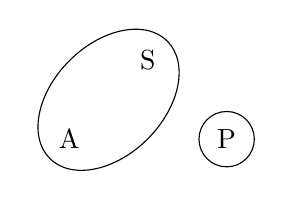
\begin{tikzpicture}
\node (S) at (1,1) {S};
\node (A) at (0,0) {A};
\node (P) at (2,0) {P};

\draw (0.5,0.5) ellipse [x radius=3em, y radius=2em, rotate=45];
\draw (P) circle [radius=1em];
\end{tikzpicture}

\a\label{ex:subject_ergabs}%
ergative--absolutive alignment (S/P---A):\medskip

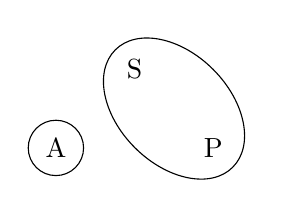
\begin{tikzpicture}
\node (S) at (1,1) {S};
\node (A) at (0,0) {A};
\node (P) at (2,0) {P};

\draw (1.5,0.5) ellipse [x radius=3em, y radius=2em, rotate=-45];
\draw (A) circle [radius=1em];
\end{tikzpicture}

\xe
\end{figure}

\citet{dixon2010} defines a subject as \textcquote[76]{dixon2010}{the entity
about which something is affirmed or denied}. He goes on to explain that,
ignoring copula clauses like `We are tired and thirsty', every language has two
varieties of clauses, intransitive ones, where the verb has just one core
argument, and transitive ones, where the verb has two core arguments. A basic
definition based on this is given by the chart in (\ref{ex:subject}). It shows
the definition of the notion of subject for both nominative--accusative
languages and ergative--absolutive languages. Languages of the world differ
based on how they prefer to treat the two nominal relations of a transitive
verb in relation to intransitive verbs: they may have a strong preference to
either treat the agent (A)---the entity that prototypically acts in some
way---or the patient/undergoer/theme (P)---the entity which is prototypically
affected by the action in some way---the same as S, the sole argument of an
intransitive verb. In the former case, the language is said to have
\Nom{}--\Acc{} alignment (\ref{ex:subject_nomacc}) with S/A being the
nominative subject, whereas in the latter case (\ref{ex:subject_ergabs}), the
language is said to have \Erg{}--\Abs{} alignment with S/P being the absolutive
subject. \citet{comrie1989} illustrates this difference with an example from
Chukchi, which we will here contrast with English:\footnote{In English,
\fw{you} is the same for both singular and plural as well as subjective and
objective case, which is why I replaced it with the unambiguous
\fw{her} in (\ref{ex:engchuk_eng}).}

\needspace{5\baselineskip}%
\pex\label{ex:engchuk_eng}
\a\label{ex:engchuk_eng1}\begingl
	\gla I came //
	\glb $\underbrace{\text{\Fsg{}.\Nom{}}}_{\text{S}}$
		come.\Pst{} //
\endgl

\a\label{ex:engchuk_eng2}\begingl
	\gla I saw her //
	\glb $\underbrace{\text{\Fsg{}.\Nom{}}}_{\text{S/A}}$
		see.\Pst{}
		$\underbrace{\text{\TsgF{}.\Obl{}}}_{\text{P}}$
		//
\endgl

\xe

\needspace{5\baselineskip}%
\pex~\label{ex:engchuk_chuk}%
Chukchi \parencite[adapted from][104]{comrie1989}:
\a\label{ex:engchuk_chuk1}\begingl
	\gla ɣəm tə-yet-ɣʔek //
	\glb $\underbrace{\text{\Fsg{}.\Abs{}}}_{\text{S}}$
		came-\Fsg{} //
	\glft `I came.' //
\endgl

\a\label{ex:engchuk_chuk2}\begingl
	\gla ɣəm-nan ɣət tə-lʔu-ɣət //
	\glb $\underbrace{\text{\Fsg{}.\Erg{}}}_{\text{A}}$
		$\underbrace{\text{\Ssg{}.\Abs{}}}_{\text{S/P}}$
		saw-\Fsg{}-\Ssg{} //
	\glft `I saw thee.' //
\endgl

\xe

While English treats the actor of the intransitive sentence
(\ref{ex:engchuk_eng1}) the same as that of the transitive one
(\ref{ex:engchuk_eng2})---both sentences use \fw{I} in the nominative---Chukchi
appears to use a different pronoun for the actor of the intransitive sentence
(\ref{ex:engchuk_chuk1}) than the actor of the transitive one
(\ref{ex:engchuk_chuk2})---absolutive \fw{ɣəm} versus ergative \fw{ɣəmnan},
respectively. At least in Standard English, it would be ungrammatical to use
the pronoun \fw{me} in place of \fw{I} in (\ref{ex:engchuk_eng2}), since
\fw{me} can only be used for first-person objects of the verb, but not for
subjects of transitive clauses.

However, \citet{comrie1989} also urges to consider that grammatical relations
and their representation in morphology are not always as clear-cut as in the
example above. While he characterizes the prototypical subject as the
intersection of agent and topic as far as cross-linguistic evidence is
concerned \citep[107]{comrie1989}, he also points out that subjects do not
necessarily have to unite all the properties typically associated with them
\citep[110]{comrie1989}. This seems to be the case, with Tagalog, for instance,
as observed by both \citet{schachter1976} and \citet{kroeger1991}, and may
considerably complicate making a definitive statement.

Moreover, \citet{comrie1989} points out that statistically, languages of the
world show a strong preference for \Nom{}--\Acc{} alignment, possibly due to
the fact that human perception values actors as more relevant to discourse than
patients, which is why actors are far more likely also to be pragmatic topics
\citep[120]{comrie1989}. Yet, though, dominantly \Nom{}--\Acc{}-aligned
languages may show a bias towards an \Erg{}--\Abs{} treatment, for instance, of
resultative constructions. On the other hand, dominantly \Erg{}--\Abs{}
languages show a bias towards a \Nom{}--\Acc{} treatment, for instance, of
addressees of imperatives \citep[116--119]{comrie1989}.

According to \citet{carnie2013}, from the point of view of constituent
structure (which is key in Generative Grammar), a subject is conventionally
understood as a \textcquote[221]{carnie2013}{DP that has the property
indicated by the predicate phrase. What the sentence is about. In most
sentences, this surfaces in the specifier of [the tense phrase]}. However, as
we have seen above, this notion is challenged by languages such as Tagalog
\citep[225]{kroeger1991}. What \citet{carnie2013} refers to in terms of
constituent structure was basically already indicated by (\ref{ex:basicsvo}),
except with different labels; the example is repeated here for convenience as
(\ref{ex:basicsvo2}). For systemic reasons, \citet{carnie2013} refers to a DP
subject which serves as the specifier of a TP. This corresponds to the subject
NP and the IP here. Unlike \textsc{gg}, \Lfg{} treats tense as a semantic
feature, not as a functional head with a fixed position in constituent
structure, hence the difference in labeling.

\begin{figure}
\ex\label{ex:basicsvo2}
\begin{forest}
[IP
	[NP
		[\textsc{subject}, roof]
	]
	[\xbar{I}
		[\xhead{I}
			[\textsc{(auxiliary)}]
		]
		[VP
			[\xbar{V}
				[\xhead{V}
					[\textsc{verb}]
				]
				[NP
					[\textsc{object}, roof]
				]
			]
		]
	]
]
\end{forest}
\xe
\end{figure}

\Lfg{} defines a subject function, \Subj{}. Which argument of the verb the
subject is mapped onto is understood to be based on the relative prominence of
the subject argument along some dimension compared to other arguments. For
instance, \Nom{}--\Acc{} languages prefer the semantically most prominent
available role of a verb's argument structure, \Erg{}--\Abs{} languages instead
pick the argument most affected by the actor's action, and active languages
focus on the argument in control of the action \citep[95--96]{bresnan2016}. The
mapping between grammatical functions like \Subj{} and the lexical components
that make it up also does not need to be a one-to-one correspondence, since
\Lfg{} allows for the distributed exponence of grammatical features like in the
example of Warlpiri in (\ref{ex:warlastruct}). The only condition is that
grammatical functions be uniquely defined within their minimal f-structure
\citep[45]{bresnan2016}. As (\ref{ex:warlastruct}) shows, multiple NPs in
different positions in the constituent structure may feed semantic information
to a single function defined by the argument structure of the verb.

\begin{figure}
\ex\label{ex:warlastruct}
\begingl[glwordalign=center]
\glpreamble Warlpiri \citep[325]{bresnan2016}: //
\gla {~\hspace{1.5em}} {} chase {\quad\normalfont ⟨} agent {\quad} patient 
{\normalfont ⟩} {} //
\glb {} {[}
	\Pred{}\tikzmark{warlastruct_Pred}
	{}
	\Subj{}\tikzmark{warlastruct_Subj}
	{}
	\Obj{}\tikzmark{warlastruct_Obj}
	{}
	{]} //
\endgl

\begin{forest}
[IP
	[{NP~\tikzmark{warlastruct_ERGNP1}}
		[{...-\Erg{}}, roof]
	]
	[\xbar{I}
		[I, minimum width=5em]
		[S, minimum width=5em
			[{\tikzmark{warlastruct_V}~V}]
			[{NP~\tikzmark{warlastruct_ABSNP1}}
				[{...-\Abs{}}, roof]
			]
			[{NP~\tikzmark{warlastruct_ERGNP2}}
				[{...-\Erg{}}, roof]
			]
			[{NP~\tikzmark{warlastruct_ABSNP2}}
				[{...-\Abs{}}, roof]
			]
		]
	]
]
\end{forest}
\begin{tikzpicture}[remember picture, overlay]
\draw [-latex, min distance=1cm]
	([yshift=1ex]{pic cs:warlastruct_V})
	to [out=west, in=south]
	([xshift=-1em, yshift=-.5ex]{pic cs:warlastruct_Pred});

\draw [-latex, min distance=1cm]
	([yshift=1ex]{pic cs:warlastruct_ERGNP1})
	to [out=east, in=south]
	([xshift=-.75em, yshift=-.5ex]{pic cs:warlastruct_Subj});
\draw [-latex, min distance=1cm]
	([yshift=1ex]{pic cs:warlastruct_ERGNP2})
	to [out=east, in=south]
	([xshift=-.75em, yshift=-.5ex]{pic cs:warlastruct_Subj});

\draw [-latex, min distance=1cm]
	([yshift=1ex]{pic cs:warlastruct_ABSNP1})
	to [out=east, in=south]
	([xshift=-.5em, yshift=-.5ex]{pic cs:warlastruct_Obj});
\draw [-latex, min distance=1cm]
	([yshift=1ex]{pic cs:warlastruct_ABSNP2})
	to [out=east, in=south]
	([xshift=-.5em, yshift=-.5ex]{pic cs:warlastruct_Obj});
\end{tikzpicture}
\xe
\end{figure}

The subject role $\hat{\theta}$ is defined as \textcquote[330]{bresnan2016}
{the most prominent semantic role of a predicator}. Furthermore,
\citet{bresnan2016} devise two a-structure features, [±\,o] (objective) and
[±\,r] (restrictive). According to this classification, \Subj{} is assigned the
features [–\,r, –\,o], since the subject is not restricted to a certain
semantic role, nor needs to have a semantic role.\footnote{This ought to make
\citet{kroeger1991}'s analysis compatible to \Lfg{} as well.} Also, subjects do
not complement transitive predicators like objects do, so they are not
`objective'. \citet{bresnan2016}'s lexical mapping theory assumes that all
languages have subjects, which goes counter to
\textcites{schachter1976}{schachter2015}'s claim that subjects are possibly not
universal \citep[330--331]{bresnan2016}.

\subsubsection{Topic}

The notion of \textbf{topic} refers essentially to who or what a longer stretch
of conversation is about. \citet{givon1983} defines the topic of a `thematic
paragraph'---as he calls a coherent unit of discourse above the level of a
single sentence---as \textcquote[8]{givon1983}{the continuity marker, the
\fw{leitmotif}}. The topic is thus

\blockcquote[8]{givon1983}{the participant \emph{most crucially involved} in
the action sequence running through the paragraph; it is the participant most
closely associated with the higher-level \enquote{theme} of the paragraph; and
finally, it is the participant most likely to be coded as the \emph{primary
topic}---or grammatical subject---of the vast majority of sequentially-ordered
clauses/sentences comprising the thematic paragraph.}

This indicates that topic and subject are closely related concepts, as already
mentioned above in reference to \citet{comrie1989}. Languages employ various
means to indicate topics; right- and left-dislocation, as known from English,
or topic-marking particles as in Japanese and Korean, are only two among many
possibilities \citep[174]{dixon2010}.

Topicality also interfaces with definiteness in that chain-initial topics may
be definite (already introduced into discourse) or indefinite (newly introduced
into discourse), while chain-medial topics and chain-final topics are always
expected to be definite \citep[10]{givon1983}. \citet[171]{dixon2010} adds that
topic NPs are coreferential with arguments of clauses immediately preceding or
following the current clause. Moreover, the strategy of passivization (in
\Nom{}--\Acc{} languages) or of antipassivization (in \Erg{}--\Abs{} languages)
exists, among others, in order to keep a certain discourse item persistent in
the highly topical subject position even if it would otherwise be the object of
the clause. This is related in turn to the notion of syntactic pivot in clause
coordination \citep[172]{dixon2010}.

\subsubsection{Focus}

Regarding the definition of \textbf{focus}, \citet[174]{dixon2010} only
mentions contrastive focus, which basically raises the prominence of a certain
NP within a single clause. It is not necessary for the focussed NP to be
coordinated with another NP by `or'. \citet{dixon2010} also warns that focus
is often confused with topic. Perhaps this is in part also, as
\citet{bresnan2016} mention, due to the fact that English may use the topic
position for either topic or focus under certain circumstances 
\parencite[98]{bresnan2016}:

\ex\label{ex:engfoc}%
Q: What did you name your cat?\\
A: \textsc{rosie} I named her. (\fw{Rosie} = \Foc{})
\xe

The answer to a \fw{wh}-question is considered focused, so \fw{Rosie} in
(\ref{ex:engfoc}) is the focus in `I named her \textsc{rosie}'. However, in the
example above, \fw{Rosie} is fronted, which following \citet{givon1983},
constitutes a disruptive action used to establish a new topic of conversation:
left-dislocation in languages with rigid SVO word order such as English is
typically associated with low topic continuity, and left-dislocated NPs can be
found most often as initiating a topic chain \citep[32]{givon1983}.

\subsection{Tests on subjecthood}
\label{subsec:subjecthood}

As initially mentioned, Ayeri was originally conceived under an impression of
what was described in the quote by \citet{cowan1995} above in terms of `trigger
language' (also compare \cite{schachter2015}). That is, in simple declarative
statements, the semantic macrorole of a definite NP is marked on the verb. This
is itself a very basic account of what can be observed in Tagalog and other
Philippine languages, compare (\ref{ex:tagmarking}) (emphasis
mine).\footnote{The underlining here is not supposed to be read as marking
contrastive focus---this is one of the `mistakes' that has led to what I have
in Ayeri, basically, besides then also mixing up focus and topic.} Further
effects will be discussed in more detail below.

\needspace{3\baselineskip}
\pex\label{ex:tagmarking}%
Tagalog (\cite[14]{kroeger1991}, adapted from \cite[135]{foleyvanvalin1984}):
\a\label{ex:tagmarking_av}\begingl
	\gla B-\textbf{um}-ili \textbf{ang=lalake} ng=isda sa=tindahan. //
	\glb \Pfv{}.\Av{}-buy \Nom{}=man \Gen{}=fish \Dat{}=store //
	\glft `\emph{The man} bought fish at the store.' //
\endgl

\a\label{ex:tagmarking_ov}\begingl
	\gla B-in-ili-\textbf{Ø} ng=lalake \textbf{ang=isda} sa=tindahan. //
	\glb \Pfv{}-buy-\Ov{} \Gen{}=man \Nom{}=fish \Dat{}=store //
	\glft `The man bought \emph{the fish} at the store.' //
\endgl

\a\label{ex:tagmarking_dv}\begingl
	\gla B-in-ilh-\textbf{an} ng=lalake ng=isda \textbf{ang=tindahan.} //
	\glb \Pfv{}-buy-\Dv{} \Gen{}=man \Gen{}=fish \Nom{}=store //
	\glft `The man bought fish \emph{at the store}.' //
\endgl

\a\label{ex:tagmarking_iv}\begingl
	\gla \textbf{Ip}-in-\textbf{am}-bili ng=lalake ng=isda 
		\textbf{ang=pera.} //
	\glb \Iv{}-\Pfv{}-buy \Gen{}=man \Gen{}=fish \Nom{}=money //
	\glft `The man bought fish \emph{with the money}.' //
\endgl

% Tagalog example is missing in Kroeger (1991), present in Kroeger (1993: 14)
% (print edition of PhD thesis, Google Books BV9O0Kk5WcMC)
% \a\label{ex:tagmarking_bv}\begingl
% 	\gla I-b-in-ili ng=lalake ng=isda \textbf{ang=bata.} //
% 	\glb \Bv{}-\Pfv{}-buy \Gen{}=man \Gen{}=fish \Nom{}=child //
% 	\glft `The man bought fish \emph{for the child}.' //
% \endgl

\xe

The examples in (\ref{ex:tagmarking}) show variations on the same sentence,
differing in the distribution of the definite NP which \citet{kroeger1991}
classifies as being the subject of the respective sentence on syntactic
grounds. The subject NPs are marked with the clitic \fw{ang}, and their role in
the clause is reflected by the voice marking on the verb (the root is \fw{bili}
`buy'): in (\ref{ex:tagmarking_av}) the subject is the actor, in
(\ref{ex:tagmarking_ov}) it is the object, in (\ref{ex:tagmarking_dv}) it is a
location, and in (\ref{ex:tagmarking_iv}) it is an instrument. What is
remarkable is that this voice marking goes beyond mere
passivization,\footnote{Note that \citet{kroeger1991} avoids the terms
\emph{active voice} and \emph{passive voice} that \citet{schachter2015} objects
to as inappropriate, even though what Tagalog does essentially appears to work
along those lines, except in a more generalized way.} so even the oblique
arguments of (\ref{ex:tagmarking}cd) can become subjects of their respective
clauses. Ayeri is at least superficially similar, compare
(\ref{ex:ayrmarking}).

\pex\label{ex:ayrmarking}
\a\label{ex:ayrmarking_at}\begingl
	\gla \textbf{ang}=int-ya \textbf{ayon-Ø} inun-ley moton-ya //
	\glb \AgtT{}=buy-\TsgM{} man-\Top{} fish-\PargI{} store-\Loc{} //
	\glft `\emph{The man}, he bought fish at the store.' //
\endgl

\a\label{ex:ayrmarking_pt}\begingl
	\gla \textbf{le}=int-ya ayon-ang \textbf{inun-Ø} moton-ya //
	\glb \PatTI{}=buy-\TsgM{} man-\Aarg{} fish-\Top{} store-\Loc{} //
	\glft `\emph{The fish}, the man bought it at the store.' //
\endgl

\a\label{ex:ayrmarking_loct}\begingl
	\gla \textbf{ya}=int-ya ayon-ang inun-ley \textbf{moton-Ø} //
	\glb \LocT{}=buy-\TsgM{} man-\Aarg{} fish-\PargI{} store-\Top{} //
	\glft `\emph{The store}, the man bought fish there.' //
\endgl

\a\label{ex:ayrmarking_inst}\begingl
	\gla \textbf{ri}=int-ya ayon-ang inun-ley \textbf{pangis-Ø} //
	\glb \InsT{}=buy-\TsgM{} man-\Aarg{} fish-\PargI{} money-\Top{} //
	\glft `\emph{The money}, the man bought fish with it.' //
\endgl

% \a\label{ex:ayrmarking_datt}\begingl
% 	\gla yam=int-ya ayon-ang inun-ley \textbf{gan-Ø} //
% 	\glb \DatT{}=buy-\TsgM{} man-\Aarg{} fish-\PargI{} child-\Top{} //
% 	\glft `\emph{The child}, the man bought fish for it.' //
% \endgl

\xe

Like Tagalog, Ayeri marks a privileged NP on the verb, however, in Ayeri, this
is the topic, not the subject (this will be subject to further scrutiny below).
Unlike in Tagalog, the marked NP is not marked by a particle, but by the very
absence of case marking on the NP itself. The marker corresponding to the role
of the topic NP appears as a clitic in the shape of the corresponding NP's case
marker in its proclitic form at the left-most edge of the clause, before the
verb (compare sections \ref{subsec:case} and \ref{sec:verbs}). While the marker
on the verb is thus related to nominal case markers in Ayeri, Tagalog uses a
number of affixes for voice marking which are not obviously related to case
markers on nouns. For instance, non-subject actors are marked by the genitive
clitic \fw{ng} (pronounced \fw{nang}), while actor voice is marked by \fw{mag-}
or \fw{-um-} \parencites[74, 78]{schachterotanes1972}[16--18]{kroeger1991}. In
Ayeri, on the other hand, non-topic animate agents are marked on NPs by
\rayr{/ANF}{-ang} or \rayr{ANF}{ang}, and animate agent-topics are marked on
the verb by \rayr{ANF}{ang} as well.

\subsubsection{Verb agreement}
\label{subsubsec:verbagr}

One of the most prominent features of Ayeri with regards to verbs and their
relation to subjects is verb agreement with 3rd-person NPs. This was already
discussed at length in \autoref{clitics_postverb_person} 
(p.~\pageref{clitics_postverb_person}\,ff.) and \autoref{sec:verbs}. Hence, I
will only give basic information here.

\citet{kroeger1991} mentions that Tagalog has optional plural agreement of
predicates with the nominative NP if the nominative argument of the clause is
plural. This is independent of whether the nominative argument is also the
actor of the clause or not \citep[24--25]{kroeger1991}, compare
(\ref{ex:tagagr}). The arrows in (\ref{ex:tagagr}) mark government and
agreement relationships: the verb governs role and case assignment (top arrow),
while the nominative NP controls plural agreement on the verb (bottom arrow).
As the arrows illustrate, the relationship between the assignment of the
subject role and thus nominative case and plural agreement on the verb are
symmetric: the verb agrees in both (\ref{ex:tagagr_1}) and (\ref{ex:tagagr_2})
with the respective nominative NP, whether it is the agent (\ref{ex:tagagr_1})
or not (\ref{ex:tagagr_2}).

\begin{figure}
\pex\label{ex:tagagr}%
Tagalog (adapted from \cite[24--25]{kroeger1991}, from 
	\cite[122--123]{aspillera1969}):
\a\label{ex:tagagr_1}\begingl[aboveglbskip=1.5em, aboveglftskip=1.75em]
	\gla nagsisi-kain na ang=mga=bata ng=hapunan //
	\glb \Av{}.\Impf{}.\Pl{}-eat\tikzmark{tagagra_targ} already 
		$\underbrace{\text{\Nom{}=\Pl{}=child}\tikzmark{tagagra_ctrl1}}_%
			{\text{S/A}\tikzmark{tagagra_ctrl2}}$
		$\underbrace{\text{\Gen{}=\smash{supper}}}_%
			{\text{P}}$ //
	\glft `The children are eating their supper already.' //
\endgl
\begin{tikzpicture}[remember picture, overlay]
\draw [-latex]
	([xshift=-.5*width{"av.impf.pl-eat"}, yshift=2.25ex]{pic cs:tagagra_targ})
	|- ++ (north:.75em) -|
	([xshift=-.5*width{"nom=pl=child"}, yshift=2.25ex]{pic cs:tagagra_ctrl1});

\draw [-latex]
	([xshift=-.5*width{"s/a"},yshift=-.75ex]{pic cs:tagagra_ctrl2}) 
	|- ++ (south:.75em) -|
	([xshift=-.5*width{"av.impf.pl-eat"}, yshift=-.75ex]{pic cs:tagagra_targ});
\end{tikzpicture}

\a\label{ex:tagagr_2}\begingl[aboveglbskip=1.5em, aboveglftskip=1.75em]
	\gla pagsu-sulat-in ni=Linda ang=mga=liham //
	\glb \Fut{}.\Pl{}-write-\Ov{}\tikzmark{tagagrb_targ}
		$\underbrace{\text{\Gen{}=Linda}}_%
			{\text{A}}$
		$\underbrace{\text{\Nom{}=\Pl{}=letter}\tikzmark{tagagrb_ctrl1}}_%
			{\text{S/P}\tikzmark{tagagrb_ctrl2}}$ //
	\glft `Linda will write the letters.' //
\endgl
\begin{tikzpicture}[remember picture, overlay]
\draw [-latex]
	([xshift=-.5*width{"fut.pl-write-ov"}, yshift=2.25ex]{pic cs:tagagrb_targ})
	|- ++ (north:.75em) -|
	([xshift=-.5*width{"nom=pl=letter"}, yshift=2.25ex]{pic cs:tagagrb_ctrl1});

\draw [-latex]
	([xshift=-.5*width{"s/p"},yshift=-.75ex]{pic cs:tagagrb_ctrl2}) 
	|- ++ (south:.75em) -|
	([xshift=-.5*width{"fut.pl-write-ov"}, yshift=-.75ex]%
		{pic cs:tagagrb_targ});
\end{tikzpicture}
\xe
\end{figure}

As described before, person agreement in Ayeri is essentially fixed to the
agent NP in canonical cases, whether it is the topic of the clause or not. In
(\ref{ex:ayragr_1}), we can see the verb determine that the agent argument is
also the topic, with the verb agreeing itself in person with the agent:
\rayr{AgYaanF}{Ajān} is a male name; the verb corresponds with masculine
agreement. In (\ref{ex:ayragr_2}), however, the relation is asymmetric in that
the marking on the verb shows that the patient argument is the topic, while the
verb still displays masculine person agreement. We know that the verb agrees
with \rayr{AgYaanF}{Ajān} rather than with \rayr{pil}{Pila} because the latter
is a female name, so the verb should have feminine agreement if it were to
agree with the patient NP. However, as the example shows, the verb continues to
agree with the agent NP in spite of not being the topic of the clause.
Topicalization appears to have no influence on the distribution of person
agreement on the verb; the agent NP remains the subject. This is a very
\Nom{}--\Acc{} trait.

\begin{figure}
\pex\label{ex:ayragr}
\a\label{ex:ayragr_1}\begingl[aboveglcskip=1.5em, aboveglftskip=1.75em]
	\gla {Ang manya} Ajān {sa Pila}. //
	\glb ang=man-ya {Ø=Ajān} {sa=Pila} //
	\glc \AgtT{}=greet-\TsgM{}\tikzmark{ayragra_targ}
		$\underbrace{\text{\Top{}=\smash{Ajān}}\tikzmark{ayragra_ctrl1}}_%
		{\text{S/A}\tikzmark{ayragra_ctrl2}}$
		$\underbrace{\text{\Parg{}=Pila}}_{\text{P}}$ //
	\glft `Ajān, he greets Pila.' //
\endgl
\begin{tikzpicture}[remember picture, overlay]
\draw [-latex]
	([xshift=-.5*width{"at=greet-3sg.m"}, yshift=2.25ex]{pic cs:ayragra_targ})
	|- ++ (north:.75em) -|
	([xshift=-.5*width{"top=Ajān"}, yshift=2.25ex]{pic cs:ayragra_ctrl1});

\draw [-latex]
	([xshift=-.5*width{"s/a"},yshift=-.75ex]{pic cs:ayragra_ctrl2}) 
	|- ++ (south:.75em) -|
	([xshift=-.5*width{"at=greet-3sg.m"}, yshift=-.75ex]{pic cs:ayragra_targ});
\end{tikzpicture}

\a\label{ex:ayragr_2}\begingl[aboveglcskip=1.5em, aboveglftskip=1.75em]
	\gla {Sa manya} {ang Ajān} Pila. //
	\glb sa=man-ya {ang=Ajān} {Ø=Pila} //
	\glc \PatT{}=greet-\TsgM{}\tikzmark{ayragrb_targ}
		$\underbrace{\text{\Aarg{}=\smash{Ajān}}}_%
			{\text{S/A}\tikzmark{ayragrb_ctrl2}}$
		$\underbrace{\text{\Top{}=Pila}\tikzmark{ayragrb_ctrl1}}_{\text{P}}$ //
	\glft `Pila, Ajān greets her.' //
\endgl
\begin{tikzpicture}[remember picture, overlay]
\draw [-latex]
	([xshift=-.5*width{"pt=greet-3sg.m"}, yshift=2.25ex]{pic cs:ayragrb_targ})
	|- ++ (north:.75em) -|
	([xshift=-.5*width{"top=Pila"}, yshift=2.25ex]{pic cs:ayragrb_ctrl1});

\draw [-latex]
	([xshift=-.5*width{"s/a"},yshift=-.75ex]{pic cs:ayragrb_ctrl2}) 
	|- ++ (south:.75em) -|
	([xshift=-.5*width{"pt=greet-3sg.m"}, yshift=-.75ex]{pic cs:ayragrb_targ});
\end{tikzpicture}

\xe
\end{figure}

In agentless clauses, however, the verb agrees with the patient argument, which
makes Ayeri less typical a \Nom{}--\Acc{} language, and more similar in this
regard to what an \Erg{}--\Abs{} language would be expected to do.
Passivization of a transitive clause as a strategy for keeping the topic
constant as a subject is essentially preempted by Ayeri's use of a topic
particle in the verb phrase. Hence, a sentence like (\ref{ex:ayragr2_1})---as a
parallel to (\ref{ex:tagagr_2})---sounds odd, while (\ref{ex:ayragr2_2}) is
fine.

\begin{figure}
\pex\label{ex:ayragr2}
\a\label{ex:ayragr2_1}\ljudge\ques%
\begingl[aboveglcskip=1.5em, aboveglftskip=1.75em]
	\gla {Sa manye} {ang Ajān} Pila. //
	\glb sa=man-ye {ang=Ajān} {Ø=Pila} //
	\glc \PatT{}=greet-\TsgF{}\tikzmark{ayragr2a_targ}
		$\underbrace{\text{\Aarg{}=\smash{Ajān}}}_{\text{A}}$
		$\underbrace{\text{\Top{}=Pila}\tikzmark{ayragr2a_ctrl1}}_%
			{\text{S/P}\tikzmark{ayragr2a_ctrl2}}$ //
	\glft `Pila, she is greeted by Ajān.' //
\endgl
\begin{tikzpicture}[remember picture, overlay]
\draw [-latex]
	([xshift=-.5*width{"pt=greet-3sg.f"}, yshift=2.25ex]{pic cs:ayragr2a_targ})
	|- ++ (north:.75em) -|
	([xshift=-.5*width{"top=Pila"}, yshift=2.25ex]{pic cs:ayragr2a_ctrl1});

\draw [-latex]
	([xshift=-.5*width{"s/p"},yshift=-.75ex]{pic cs:ayragr2a_ctrl2}) 
	|- ++ (south:.75em) -|
	([xshift=-.5*width{"pt=greet-3sg.f"}, yshift=-.75ex]%
		{pic cs:ayragr2a_targ});
\end{tikzpicture}

\a\label{ex:ayragr2_2}\begingl[aboveglftskip=1.75em]
	\gla Manye {sa Pila}. //
	\glb man-ye Ø=Pila //
	\glc greet-\TsgF{}\tikzmark{ayragr2b_targ}
		$\underbrace{\text{\Parg{}=Pila}}_%
			{\text{S/P}\tikzmark{ayragr2b_ctrl}}$ //
	\glft `Pila is greeted.' //
\endgl
\begin{tikzpicture}[remember picture, overlay]
\draw [-latex]
	([xshift=-.5*width{"s/p"},yshift=-.75ex]{pic cs:ayragr2b_ctrl}) 
	|- ++ (south:.75em) -|
	([xshift=-.5*width{"pt=greet-3sg.f"}, yshift=-.75ex]%
		{pic cs:ayragr2b_targ});
\end{tikzpicture}

\xe
\end{figure}

\subsubsection{Syntactic pivot}
\label{subsubsec:pivot}

Since we have just dealt with aspects of syntactic alignment and found that
Ayeri behaves a little oddly with regards to this, it may be interesting to
perform another test on declarative statements and their syntactic pivot as
well. A simple test which \citet[111--114]{comrie1989} describes in this regard
is to test coreference in coordinated clauses. In coordinated clauses, it seems
to be not uncommon for the subject of the second conjunct to drop out. Thus, in
English, which behaves very much in terms of \Nom{}--\Acc{} alignment in this
regard, we get the following result:

\pex[belowexskip=1.75em]\label{ex:engpivot}%
%	English:
	\a\label{ex:engpivot_1}%
		$\underbrace{The\ cat}_{\text{A}}$ 
		$hunts$ $\underbrace{the\ mouse}_{\text{P}}$.
	
	\a\label{ex:engpivot_2}%
		$\underbrace{The\ cat}_{\text{S}}$ $comes\ here.$
	
	\a\label{ex:engpivot_3}%
		$\underbrace{The\ mouse}_{\text{S}}$ $comes\ here.$
	
	\a\label{ex:engpivot_4}%
		$\underbrace{The\ cat}_{\text{A}\tikzmark{engpivot_ant}}$
		$hunts$
		$\underbrace{the\ mouse}_{\text{P}}$
		$and$
		$\underbrace{ }_{\text{S}\tikzmark{engpivot_drop}}$
		$comes\ here.$

\begin{tikzpicture}[remember picture, overlay]
\draw [-latex] ([xshift=-.25em,yshift=-.75ex]{pic cs:engpivot_ant}) 
|- ++ (south:.75em) -| ([xshift=-.25ex, yshift=-.75ex]{pic cs:engpivot_drop});
\end{tikzpicture}
\xe

In the English example in (\ref{ex:engpivot}), \fw{the cat} constitutes the
coreferential subject in (\ref{ex:engpivot_4}). This NP is the intransitive
subject S of (\ref{ex:engpivot_2}) and the agent A of (\ref{ex:engpivot_1}).
English thus typically has \Nom{}--\Acc{} alignment, since it treats S and A
alike. In an \Erg{}--\Abs{} language, then, we would expect the opposite case:
S and P should be treated alike. In Dyirbal, we find the situation depicted by
the examples in (\ref{ex:dyirpivot}).

\begin{figure}
\pex\label{ex:dyirpivot}%
Dyirbal \parencite[adapted from][112]{comrie1989}:
\a\label{ex:dyirpivot_1}
	\begingl
		\gla {balan dʸugumbil} {baŋgul yaṛaŋgu} balgan //
		\glb $\underbrace{\text{\Det{} woman-\Abs{}}}_{\text{P}}$
			$\underbrace{\text{\Det{} man-\Erg{}}}_{\text{A}}$ hit //
		\glft `The man hit the woman.' //
	\endgl
	
\a\label{ex:dyirpivot_2}%
	\begingl
		\gla {bayi yaṛa} baninʸu //
		\glb $\underbrace{\text{\Det{} man-\Abs{}}}_{\text{S}}$ came.here //
		\glft `The man came here.' //
	\endgl
	
\a\label{ex:dyirpivot_3}%
	\begingl
		\gla {balan dʸugumbil} baninʸu //
		\glb $\underbrace{\text{\Det{} woman-\Abs{}}}_{\text{S}}$ 
			came.here //
		\glft `The woman came here.' //
	\endgl
	
\a\label{ex:dyirpivot_4}%
	\begingl[aboveglftskip=1.75em]
		\gla {balan dʸugumbil} {baŋgul yaṛaŋgu} balgan, {} baninʸu //
		\glb $\underbrace{\text{\Det{} woman-\Abs{}}}_%
				{\text{P}\tikzmark{dyirpivot_ant}}$
			$\underbrace{\text{\Det{} man-\Erg{}}}_{\text{A}}$
			hit 
			$\underbrace{ }_{\text{S}\tikzmark{dyirpivot_drop}}$
			came.here //
		\glft `The man hit the woman, and [the woman] came here.' //
	\endgl

\begin{tikzpicture}[remember picture, overlay]
\draw [-latex] ([xshift=-.25em,yshift=-.75ex]{pic cs:dyirpivot_ant}) 
|- ++ (south:.75em) -| ([xshift=-.25ex, yshift=-.75ex]{pic cs:dyirpivot_drop});
\end{tikzpicture}
\xe
\end{figure}

In (\ref{ex:dyirpivot}), we find that \fw{balan dʸugumbil} `the woman' is
coreferential in (\ref{ex:dyirpivot_4}). This is the S of
(\ref{ex:dyirpivot_3}), and the P of (\ref{ex:dyirpivot_1}). Dyirbal, thus,
treats S and P alike, as predicted for an \Erg{}--\Abs{} language---at least in
this case, since \citet[113]{comrie1989} also explains that \Fsg{} and \Ssg{}
pronouns in Dyirbal behave in terms in terms of \Nom{}--\Acc{}.
\citet{comrie1989} also notes that some languages do not show a clear
preference for whether the A or P of the transitive clause in the first
conjunct is the preferred reference of the S of the intransitive clause in the
second conjunct.

For Tagalog, as \citet{kroeger1991} explains, \textcquote[30]{kroeger1991}{the
deletion is not obligatory but null nominative arguments are always interpreted
as referring to the nominative argument of the main clause}. Due to the way
Tagalog treats subjects, however, the nominative argument can be formed by
either NP in (\ref{ex:tagpivot}) with the voice marked accordingly on the
verb.\footnote{Thus, compare the English passive sentence \fw{Marvin$_i$ was
asked by Derek$_j$ before he$_i$ left} with (\ref{ex:tagpivot_1}). In English,
the reference of \fw{he} is ambiguous between the syntactic subject \fw{Marvin}
and the agent \fw{Derek}, however. As we have seen above, though, Tagalog would
also be able to make a subject of an oblique argument, not just of the
patient/theme or the recipient. The actor of the Tagalog sentence is also
basically an object, not demoted to an adverbial as in English
\citep[38--44]{kroeger1991}.}

\begin{figure}
\pex\label{ex:tagpivot}%
Tagalog (\cite[adapted from][31]{kroeger1991}, from 
	\cite[151--152]{ramoscena1990}):
\a\label{ex:tagpivot_1}%
\begingl[aboveglbskip=1.5em, aboveglftskip=1.75em]
	\gla tinanong ni=Derek si=Marvin, bago umalis {} //
	\glb \Pfv{}-ask-\Ov{}\tikzmark{tagpivot1_vc}
		$\underbrace{\text{\Gen{}=Derek}}_{\text{A}}$
		$\underbrace{\text{\Nom{}=Marvin}\tikzmark{tagpivot1_anta}}_%
			{\text{P}\tikzmark{tagpivot1_antb}}$
		before \Pfv{}.\Av{}-leave\tikzmark{tagpivot1_vc2}
		$\underbrace{ \tikzmark{tagpivot1_anta2}}_%
			{\text{S}\tikzmark{tagpivot1_drop}}$
		//
	\glft `Derek asked Marvin before [Marvin] left.' //
\endgl
\begin{tikzpicture}[remember picture, overlay]
\draw [-latex] 
	([xshift=-.5*width{"pfv-ask-ov"},yshift=+2.25ex]{pic cs:tagpivot1_vc})
	|- ++ (north:.75em) -|
	([xshift=-.5*width{"nom=Marvin"}, yshift=2.25ex]{pic cs:tagpivot1_anta});

\draw [-latex]
	([xshift=-.125em,yshift=-.75ex]{pic cs:tagpivot1_antb}) 
	|- ++ (south:.75em) -|
	([xshift=-.25ex, yshift=-.75ex]{pic cs:tagpivot1_drop});

\draw [-latex] 
	([xshift=-.5*width{"pfv.av-leave"},yshift=+2.25ex]{pic cs:tagpivot1_vc2})
	|- ++ (north:.75em) -|
	([xshift=0ex, yshift=2.25ex]{pic cs:tagpivot1_anta2});
\end{tikzpicture}

\a\label{ex:tagpivot_2}%
\begingl[aboveglbskip=1.5em, aboveglftskip=1.75em]
	\gla nagtanong si=Derek kay=Marvin, bago umalis {} //
	\glb \Pfv{}.\Av{}-ask\tikzmark{tagpivot2_vc}
		$\underbrace{\text{\Nom{}=Derek}\tikzmark{tagpivot2_anta}}_%
			{\text{A}\tikzmark{tagpivot2_antb}}$
		$\underbrace{\text{\Dat{}=Marvin}}_{\text{P}}$
		before \Pfv{}.\Av{}-leave\tikzmark{tagpivot2_vc2}
		$\underbrace{ \tikzmark{tagpivot2_anta2}}_%
			{\text{S}\tikzmark{tagpivot2_drop}}$
		//
	\glft `Derek asked Marvin before [Derek] left.' //
\endgl
\begin{tikzpicture}[remember picture, overlay]
\draw [-latex] 
	([xshift=-.5*width{"pfv.av-ask"},yshift=+2.25ex]{pic cs:tagpivot2_vc})
	|- ++ (north:.75em) -|
	([xshift=-.5*width{"nom=Derek"}, yshift=2.25ex]{pic cs:tagpivot2_anta});

\draw [-latex]
	([xshift=-.125em,yshift=-.75ex]{pic cs:tagpivot2_antb}) 
	|- ++ (south:.75em) -|
	([xshift=-.25ex, yshift=-.75ex]{pic cs:tagpivot2_drop});

\draw [-latex] 
	([xshift=-.5*width{"pfv.av-leave"},yshift=+2.25ex]{pic cs:tagpivot2_vc2})
	|- ++ (north:.75em) -|
	([xshift=0ex, yshift=2.25ex]{pic cs:tagpivot2_anta2});
\end{tikzpicture}

\xe
\end{figure}

What can be observed in Tagalog is that in (\ref{ex:tagpivot_1}), the dropped S
argument in the second conjunct, \fw{bago umalis ...} `before ...\ leaves', is
coreferential with \fw{Marvin}, since he is marked as the subject of the first
conjunct. Since \fw{Marvin} is the theme (P) of \fw{tanong} `ask', the clause
needs to be marked for objective voice. On the other hand, in
(\ref{ex:tagpivot_2}), it is \fw{Derek} who is the subject of the clause, so it
is also he who leaves; the verb in the first conjunct clause is marked for
active voice according to the asker as the actor (A) being the subject.

In order to now investigate what the situation is in Ayeri, let us return to
our initial set of examples. These examples feature two animals which are
treated both as animate neuters. Anaphoric reference is thus potentially
ambiguous between \xayr{prlF}{paral}{cat} and \xayr{pFrbr}{prabara}{mouse}.

\pex\label{ex:ayrpivot}%
\a\label{ex:ayrpivot_1}
	\begingl
		\gla Ang @ kimbyo paral prabarās. //
		\glb ang= kimb-yo paral-Ø prabara-as //
		\glc \AgtT{}= hunt-\TsgN{}
			$\underbrace{\text{cat-\Top{}}}_{\text{A}}$
			$\underbrace{\text{mouse-\Parg{}}}_{\text{P}}$ //
		\glft `The cat hunts the mouse.' //
	\endgl
	
\a\label{ex:ayrpivot_2}%
	\begingl
		\gla Sahayo paralang edaya. //
		\glb saha-yo paral-ang edaya //
		\glc come-\TsgN{} $\underbrace{\text{cat-\Aarg{}}}_{\text{S}}$
			here //
		\glft `The cat comes here.' //
	\endgl
	
\a\label{ex:ayrpivot_3}%
	\begingl
		\gla Sahayo prabarāng edaya. //
		\glb saha-yo prabara-ang edaya //
		\glc come-\TsgN{} $\underbrace{\text{mouse-\Aarg{}}}_{\text{S}}$
			here //
		\glft `The mouse comes here.' //
	\endgl
	
\a\label{ex:ayrpivot_4}%
	\begingl[aboveglftskip=1em]
		\gla Ang @ kimbyo paral prabarās nay sahayong edaya. //
		\glb ang= kimb-yo paral-Ø prabara-as nay saha=yong edaya  //
		\glc \AgtT{}= hunt-\TsgN{}
			$\underbrace{\text{cat-\Top{}}}_{\text{A}\tikzmark{ayrpivot_ctrl}}$
			$\underbrace{\text{mouse-\Parg{}}}_{\text{P}}$
			and
			come=$\underbrace{\text{\smash{\TsgN{}}.\Aarg{}}}_%
				{\text{S}\tikzmark{ayrpivot_targ}}$
			here //
		\glft `The cat, it hunts the mouse, and it comes here.' //
	\endgl

\begin{tikzpicture}[remember picture, overlay]
\draw [-latex]
	([xshift=-.25em,yshift=-.75ex]{pic cs:ayrpivot_ctrl}) 
	|- ++ (south:.75em) -|
	([xshift=-.25em,yshift=-.75ex]{pic cs:ayrpivot_targ});
\end{tikzpicture}
\xe

While it is possible in Ayeri to not repeat the coreferential NP in a conjunct
clause verbatim, Ayeri still appears to avoid an empty subject slot. Thus, the
verb \xayr{shyoNF}{sahayong}{it comes} in (\ref{ex:ayrpivot_4}) displays a
pronominal clitic, \xayr{/yoNF}{-yong}{it}, which constitutes the resumptive
subject pronoun of the clause. In (\ref{ex:ayrpivot_4}) at least, this pronoun
is coreferential with the subject in the first conjunct,
\xayr{prlF}{paral}{cat}. Seeing as Tagalog switches the subject around by
altering the voice marking on the verb, it is certainly illustrative to check
how Ayeri fares if the topic is swapped to \xayr{pFrbr}{prabara}{mouse}.

\ex\label{ex:ayrpivot2}
\begingl[aboveglftskip=1em]
	\gla Sa @ kimbyo paralang prabara nay sahayong edaya. //
	\glb sa= kimb-yo paral-ang prabara-Ø nay saha=yong edaya  //
	\glc \PatT{}= hunt-\TsgN{}
		$\underbrace{\text{cat-\Aarg}}_{\text{A}}$
		$\underbrace{\text{mouse-\Top{}}}_{\text{P}\tikzmark{ayrpivot2_ctrl}}$
		and
		come=$\underbrace{\text{\smash{\TsgN{}}.\Aarg{}}}_%
			{\text{S}\tikzmark{ayrpivot2_targ}}$
		here //
	\glft `The mouse, the cat hunts it, and it comes here.' //
\endgl

\begin{tikzpicture}[remember picture, overlay]
\draw [-latex]
	([xshift=-.25em,yshift=-.75ex]{pic cs:ayrpivot2_ctrl}) 
	|- ++ (south:.75em) -|
	([xshift=-.25em,yshift=-.75ex]{pic cs:ayrpivot2_targ});
\end{tikzpicture}
\xe

In (\ref{ex:ayrpivot2}), the resumptive pronoun is indicated to not refer to
the first conjunct's agent/subject, \rayr{prlF}{paral}, but to its
theme/object, \rayr{pFrbr}{prabara}. This may be explained by topicalization:
the sentence is about the mouse, so the underspecified argument in the second
conjunct, in absence of topic marking that would indicate otherwise,
corresponds to the topic. Interestingly, the result is structurally similar to
the example of Tagalog in (\ref{ex:tagpivot}) above. It is too early yet,
however, to conclude that what was called `topic' so far is the subject; Ayeri
is merely not completely unambiguous in this context. Since Tagalog allows any
NP of a clause to be the subject, as illustrated by (\ref{ex:tagmarking}), let
us test whether the behavior just described for Ayeri also holds in other
contexts of topicalization. The following example presents sentences of
differently case-marked topic NPs each, but in every case, the agent NP and the
topicalized NP consist of a human referent. Both referents share the same
person features so that the verb in the coordinated intransitive clause can
theoretically license either of them as its antecedent.

\begin{figure}
\pex\label{ex:ayrpivot3}
\a\label{ex:ayrpivot3_dat}\begingl
	\gla Yam @ ilya ang @ Akan ilonley {} @ Maran nay sarayāng. //
	\glb yam= il-ya ang= Akan ilon-ley Ø= Maran nay sara=yāng //
	\glc \DatT{}= give-\TsgM{} \Aarg{}= Akan present-\PargI{} \Top{}= Maran
		and leave=\TsgM{}.\Aarg{} //
	\glft `Maran, Akan gives him a present, and he leaves.' (Maran leaves) //
\endgl

\a\label{ex:ayrpivot3_gen}\begingl
	\gla Na @ pahya ang @ Maran ilonley {} @ Diyan nay sarayāng. //
	\glb na= pah-ya ang= Maran ilon-ley Ø= Diyan nay sara=yāng //
	\glc \GenT{}= take.away-\TsgM{} \Aarg{}= Maran present-\PargI{} \Top{}=
		Diyan and leave=\TsgM{}.\Aarg{} //
	\glft `Diyan, Maran takes the present away from him, and he leaves.' (Diyan
		leaves) //
\endgl

\a\label{ex:ayrpivot3_loc}\begingl
	\gla Ya @ bahaya ang @ Diyan {} @ Maran nay sarayāng. //
	\glb ya= baha-ya ang= Diyan Ø= Maran nay sara=yāng //
	\glc \LocT{}= baha-\TsgM{} \Aarg{}= Diyan \Top{}= Maran and 
		leave=\TsgM{}.\Aarg{} //
	\glft `Maran, Diyan shouts at him, and he leaves.' (Maran leaves) //
\endgl

\a\label{ex:ayrpivot3_ins}\begingl
	\gla Ri @ su-sunca ang @ Diyan ilonley {} @ Sedan nay sarayāng. //
	\glb ri= su\til{}sunt-ya ang= Diyan ilon-ley Ø= Sedan nay sara=yāng. //
	\glc \InsT{}= \Iter{}\til{}claim-\TsgM{} \Aarg{}= Diyan present-\PargI{}
		\Top{}= Sedan and leave=\TsgM{}.\Aarg{} //
	\glft `Sedan, Diyan reclaims the present with his help, and he leaves.'
		(Sedan leaves) //
\endgl

\a\label{ex:ayrpivot3_cau}\begingl
	\gla Sā @ pinyaya ang @ Maran tatamanyam {} @ Sedan nay sarayāng. //
	\glb sā= pinya-ya ang= Maran tataman-yam Ø= Sedan nay sara=yāng //
	\glc \CauT{}= ask-\TsgM{} \Aarg{}= Maran forgiveness-\Dat{} \Top{}= Sedan
		and leave=\TsgM{}.\Aarg{} //
	\glft `Sedan, he makes Maran ask for forgiveness, and he leaves.' (Sedan
		leaves) //
\endgl

\xe
\end{figure}

In each of the sentences in (\ref{ex:ayrpivot3}), it is the topicalized NP
which is identified as the antecedent for \xayr{sryaaNF}{sarayāng}{he leaves}.
Does this mean Ayeri does, in fact, use Austronesian alignment? While the above
examples certainly suggest it, let us not forget that the verb in the
coordinated clause could theoretically pick either the agent NP or the
topicalized NP as its controller. Things look slightly different, however, if
the reference of the verb is unambiguous, for instance, because the topicalized
argument cannot logically be the agent of the coordinated clause:

\ex\label{ex:ayrpivot4}\begingl[aboveglcskip=1.5em, aboveglftskip=2.5em]
	\gla {Le ilya} {ang Akan} ilon {yam Maran} nay sarayāng. //
	\glb {le=il-ya} {ang=Akan} ilon-Ø {\Dat{}=Maran} nay sara=yāng //
	\glc \PatTI{}=give-\TsgM{}\tikzmark{ayrpivot4_top}
		$\underbrace{\text{\Aarg{}=Akan}}_{\text{A}\tikzmark{ayrpivot4_ctrl}}$
		$\underbrace{\text{\smash{present}-\Top{}}\tikzmark{ayrpivot4_top2}}_%
			{\text{P}\tikzmark{ayrpivot4_ctrl2}}$
		$\underbrace{\text{\Dat{}=Maran}}_{\text{R}}$
		and
		leave=$\underbrace{\text{\smash{\TsgM{}}.\Aarg{}}}_%
			{\text{S}\tikzmark{ayrpivot4_targ}}$
		//
	\glft `The present, Akan gives it to Maran, and he leaves.' 
		(Akan leaves) //
\endgl
\begin{tikzpicture}[remember picture, overlay]
\draw [-latex] 
	([xshift=-.5*width{"pt.inan=give-3sg.m"},yshift=+2.25ex]
		{pic cs:ayrpivot4_top})
	|- ++ (north:.75em) -|
	([xshift=-.5*width{"present-top"},yshift=2.25ex]{pic cs:ayrpivot4_top2});

\draw [-latex]
	([xshift=-.125em,yshift=-.75ex]{pic cs:ayrpivot4_ctrl}) 
	|- ++ (south:.75em) -|
	([xshift=-.25ex, yshift=-.75ex]{pic cs:ayrpivot4_targ});

\draw [-latex, dashed]
	([xshift=-.125em,yshift=-.75ex]{pic cs:ayrpivot4_ctrl2}) 
	|- ++ (south:1.5em) -|
	([xshift=-.25ex, yshift=-.75ex]{pic cs:ayrpivot4_targ});

\node (a) at ([yshift={-.75ex - 1.5em}]{pic cs:ayrpivot4_ctrl2}) {};
\node (b) at ([yshift={-.75ex - 1.5em}]{pic cs:ayrpivot4_targ}) {};
\node (x) at ($(a)!0.5!(b)$) {\bfseries\larger ×};
\end{tikzpicture}
\xe

In (\ref{ex:ayrpivot4}), the first conjunct's verb, as the head of its clause,
specifies that the topic of the clause is the patient (P), which is embodied by
\xayr{IlonF}{ilon}{present}. This NP, however, is not a very typical agent for
the verb in the second conjunct, \xayr{sr/}{sara-}{leave}. Besides, this verb
is conjugated so as to require an animate masculine controller, whereas
\rayr{IlonF}{ilon} is inanimate, as shown by the topic marker \rayr{le}{le}.
\rayr{IlonF}{ilon} is thus not a suitable controller for \rayr{sryaaNF}
{sarayāng}, since their person-feature values clash with each other---the 
\Anim{} and \Gend{} values in particular:

\begin{morphlex}
\pex
\a \adjustbox{valign=t}{%
\begin{tabu} {\usetabu{morphlex}}
\rayr{\larger IlonF}{ilon}
	& N
	& \begin{tabular}[t]{l l l}
		\ups{\Pred} & = & `present' \\
		\ups{\Index} & = & ↓ \\
		\quad\downs{\Pers} & = & \Third \\
		\quad\downs{\Num} & = & \Sg{} \\
		\textbf{\quad\downs{\Anim}} & \textbf{=} & \textbf{$-$} \\
		\textbf{\quad\downs{\Gend}} & \textbf{=} & \textbf{\Inan} \\
	\end{tabular}
\end{tabu}%
}

\a\adjustbox{valign=t}{%
\begin{tabu} {\usetabu{morphlex}}
\rayr{\larger sryaaNF}{sarayāng}
	& I
	& \begin{tabular}[t]{l l l}
		\ups{\Pred} & = & \astruct{leave}{\ups{\Subj}} \\
		\ups{\Subj} & = & ↓ \\
		\quad\downs{\Pred} & = & `$pro$' \\
		\quad\downs{\Pers} & = & \Third \\
		\quad\downs{\Num} & = & \Sg \\
		\textbf{\quad\downs{\Anim}} & \textbf{=} & \textbf{$+$} \\
		\textbf{\quad\downs{\Gend}} & \textbf{=} & \textbf{\M} \\
		\quad\downs{\Case} & = & \Aarg \\
	\end{tabular}
\end{tabu}%
}
\xe
\end{morphlex}

As before, there are two masculine NPs in the first conjunct which form
suitable antecedents on behalf of being animate masculine as required: the
agent (A) \rayr{AknF}{Akan} and the recipient (R) \rayr{mrnF}{Maran}. Of the
remaining non-topic NPs, Ayeri considers the agent to rank higher as a
secondary topic on the thematic hierarchy than the recipient. The agent hence
forms the preferred controller for \rayr{sryaaNF}{sarayāng}.

\ex Thematic hierarchy \citep[329]{bresnan2016}:\medskip \\
	agent > beneficiary > experiencer/goal > instrument > patient/theme >
	locative
\xe

In cases where the topic in the first conjunct can safely be ruled out as the
controller of the pronominal in the second conjunct, the syntactic pivot, thus,
defaults to the highest-ranking semantically coherent NP. In most cases,
Ayeri will therefore group the intransitive subject and the transitive agent
together. For most verbs, this is also reflected by case marking, as we have
seen above in (\ref{ex:ayrpivot}): the S of an intransitive clause receives the
same case marker as the A of a transitive clause:
\rayr{/ANF}{-ang}/\rayr{ANF}{ang} for animate referents, and
\rayr{/reNF}{reng}/\rayr{ENF}{eng} for inanimate referents (compare
\autoref{subsubsec:agent}). The case described initially, where the topic
marking basically determines the controller of the coordinated intransitive
clause, which is reminiscent of Tagalog's syntax, is essentially a strategy to
disambiguate between two possible controllers for the same target.

When only one of the referents in the transitive conjunct is eligible as the
controller of the subject of the intransitive conjunct at the same time, A and
P are regularly indicated by person agreement, since Ayeri requires a
resumptive pronominal clitic in the intransitive clause, as indicated above.
The affix on the verb thus has the status of a pronominal predicator, compare 
(\ref{ex:ayrpivot5}).

\begin{figure}
\pex\label{ex:ayrpivot5}
\a\label{ex:ayrpivot5_1}\begingl[aboveglftskip=2.5em]
	\gla Ang @ tinisaya Lita {sa Kumang} nay sarayāng. //
	\glb ang= tinisa-ya Ø=Lita sa=Kumang nay sara=yāng //
	\glc \AgtT{}= hug-\TsgM{}
		$\underbrace{\text{\Top{}=Lita}}_{\text{A}\tikzmark{ayrpivot5a_ctrl1}}$
		$\underbrace{\text{\Parg{}=\smash{Kumang}}}_%
			{\text{P}\tikzmark{ayrpivot5a_ctrl2}}$
		and 
		leave=$\underbrace{\text{\smash{\TsgM{}}.\Aarg{}}}_%
			{\text{S}\tikzmark{ayrpivot5a_targ}}$ //
	\glft `Lita, he hugs Kumang, and he leaves.' //
\endgl
\begin{tikzpicture}[remember picture, overlay]
\draw [-latex]
	([xshift=-.125em,yshift=-.75ex]{pic cs:ayrpivot5a_ctrl1}) 
	|- ++ (south:.75em) -|
	([xshift=-.25ex, yshift=-.75ex]{pic cs:ayrpivot5a_targ});

\draw [-latex, dashed]
	([xshift=-.125em,yshift=-.75ex]{pic cs:ayrpivot5a_ctrl2}) 
	|- ++ (south:1.5em) -|
	([xshift=-.25ex, yshift=-.75ex]{pic cs:ayrpivot5a_targ});

\node (a) at ([yshift={-.75ex - 1.5em}]{pic cs:ayrpivot5a_ctrl2}) {};
\node (b) at ([yshift={-.75ex - 1.5em}]{pic cs:ayrpivot5a_targ}) {};
\node (x) at ($(a)!0.5!(b)$) {\bfseries\larger ×};
\end{tikzpicture}

\a\label{ex:ayrpivot5_2}\begingl[aboveglftskip=2.5em]
	\gla Ang @ tinisaya Lita {sa Kumang} nay sarayeng. //
	\glb ang= tinisa-ya Ø=Lita sa=Kumang nay sara=yeng //
	\glc \AgtT{}= hug-\TsgM{}
		$\underbrace{\text{\Top{}=Lita}}_{\text{A}\tikzmark{ayrpivot5b_ctrl1}}$
		$\underbrace{\text{\Parg{}=\smash{Kumang}}}_%
			{\text{P}\tikzmark{ayrpivot5b_ctrl2}}$
		and 
		leave=$\underbrace{\text{\smash{\TsgF{}}.\Aarg{}}}_%
			{\text{S}\tikzmark{ayrpivot5b_targ}}$ //
	\glft `Lita, he hugs Kumang, and she leaves.' //
\endgl

\begin{tikzpicture}[remember picture, overlay]
\draw [-latex]
	([xshift=-.125em,yshift=-.75ex]{pic cs:ayrpivot5b_ctrl2}) 
	|- ++ (south:1.5em) -|
	([xshift=-.25ex, yshift=-.75ex]{pic cs:ayrpivot5b_targ});

\draw [-latex, dashed]
	([xshift=-.125em,yshift=-.75ex]{pic cs:ayrpivot5b_ctrl1}) 
	|- ++ (south:.75em) -|
	([xshift=-.25ex, yshift=-.75ex]{pic cs:ayrpivot5b_targ});

\node (a) at ([yshift={-.75ex - .75em}]{pic cs:ayrpivot5b_ctrl1}) {};
\node (b) at ([yshift={-.75ex - .75em}]{pic cs:ayrpivot5b_targ}) {};
\node (x) at ($(a)!0.5!(b)$) {\bfseries\larger ×};
\end{tikzpicture}
\xe
\end{figure}

In (\ref{ex:ayrpivot5_1}), the verb in the second conjunct, \xayr{sryaaNF}
{sarayāng}{he leaves} is marked for a masculine third-person subject. The only
available controller in the first con\-junct is \rayr{lit}{Lita} on behalf of
being male, since \rayr{kumNF}{Kumang} is female. Hence, in
(\ref{ex:ayrpivot5_2}) the verb of the intransitive conjunct, \xayr{sryeNF}
{sarayeng}{she leaves}, finds its controller only in \rayr{kumNF}{Kumang}.

\subsubsection{Quantifier float}
\label{subsubsec:quantfloat}

Another property usually associated with subjects is the ability of quantifiers
referring to the subject NP to `float' into the VP. This is possible also in
English, consider, for instance:

\pex\label{ex:engqfloat}%
% English:
\a\label{ex:engqfloat_1}%
	\fw{\textbf{All} the children are writing letters.}
\a\label{ex:engqfloat_2}%
	\fw{The children are \textbf{all} writing letters.}
\xe

Both of these sentences are equal in meaning: for all children in the set,
every child is writing an unspecified amount of letters. It is not the case in
(\ref{ex:engqfloat_2}) that for an unspecified amount of children, together
they write the total amount of letters. \fw{All} refers to \fw{the children} in
both cases, even though \fw{all} is not placed in the subject NP, \fw{the
children}, in (\ref{ex:engqfloat_2}). \citet{kroeger1991} mentions an example
from \citet{schachterotanes1972} concerning \fw{lahat} `all', which is also
able to float into a position right after the sentence-initial verb from the NP
it normally modifies and which it would normally occur in:

\pex\label{ex:tagqfloat}%
Tagalog (adapted from \cite[22]{kroeger1991}, from 
	\cite[501]{schachterotanes1972}):
\a\label{ex:tagqfloat_1}\begingl
	\gla sumusulat lahat ang=mga=bata ng=mga=liham //
	\glb \Av{}.\Impf{}-write all \Nom{}=\Pl{}=child \Gen{}=\Pl{}=letter //
	\glft `All the children are writing letters.'\\
		\textit{Not:} *`The children are writing all the letters.' //
\endgl

\a\label{ex:tagqfloat_2}\begingl
	\gla sinusulat lahat ng=mga=bata ang=mga=liham //
	\glb \Impf{}-write-\Ov{} all \Gen{}=\Pl{}=child \Nom{}=\Pl{}=letter //
	\glft `The/some children write all the letters.'\\
		\textit{Not:} *`All the children are writing letters.' //
\endgl

\xe

In (\ref{ex:tagqfloat_1}), \fw{lahat} `all' refers to the children, which
constitute the subject NP according to voice and case marking, while we get the
opposite case in (\ref{ex:tagqfloat_2}), where it refers to the letters, which
are marked as the subject this time. Of course, it is equally possible in
English to say \fw{The letters are all written by the children}, where \fw{the
letters} is the subject that the floated \fw{all} refers to.

As pointed out in \autoref{subsec:quantifiers}, a lot of clitic quantifiers in
Ayeri have a double meaning as intensifiers. For instance, \rayr{/IknF}{-ikan}
can refer to both quantities and qualities, meaning `much, many' or `very'
depending on context. Thus, many of the suffixed quantifiers, if appended to
the VP, are understood to modify the verb as an intensifier and are thus
unsuitable for floating. The only exception is \xayr{/ArilF}{-aril}{some},
which only pertains to NPs as a quantifier. However, since the floating of
suffixed quantifiers would produce readings which are ambiguous at best,
floating of \rayr{/ArilF}{-aril} is avoided as well. Example
(\ref{ex:ayrqfloat1}) shows an attempt to float \xayr{/henF}{-hen}{all} into
the IP, resulting in a meaning different from the sentence with the unfloated
particle for the reasons just stated above.

\pex\label{ex:ayrqfloat1}
\a\label{ex:ayrqfloat1_1}\begingl
	\gla Ang @ tahanyan ganye-hen tamanyeley. //
	\glb ang= tahan-yan gan-ye-Ø=hen taman-ye-ley //
	\glc \AgtT{}= write-\TplM{} child-\Pl{}-\Top{}=all letter-\Pl{}-\PargI{} //
	\glft `The children, all of them are writing letters.' //
\endgl

\a\label{ex:ayrqfloat1_2}\ljudge\excl\begingl
	\gla Ang @ tahanyan-hen ganye tamanyeley. //
	\glb ang= tahan-yan=hen gan-ye-Ø taman-ye-ley //
	\glc \AgtT{}= write-\TplM{}=completely child-\Pl{}-\Top{}
		letter-\Pl{}-\PargI{} //
	\glft `The children, they are completely writing letters.'\\
		\textit{Intended:} `The children, they are all writing letters.' //
\endgl

\xe

Besides suffixed quantifiers, Ayeri also has free quantifiers like \xayr{sno}
{sano}{both} or \xayr{diriNF}{diring}{several}, however. These free morphemes
only have a quantifying reading, not an intensifying one, and are thus suitable
for floating, since they do not produce ambiguities with regards to
what is being modified.

\pex\label{ex:ayrqfloat2}
\a\label{ex:ayrqfloat2_1}\begingl
	\gla Ang @ apayan yan sano layjya. //
	\glb ang= apa-yan yan-Ø sano lay-ye-ya //
	\glc \AgtT{}= laugh-\TplM{} boy-\Top{} both girl-\Pl{}-\Loc{} //
	\glft `The boys, both of them are laughing at the girls.' //
\endgl

\a\label{ex:ayrqfloat2_2}\begingl
	\gla Ang @ apayan sano yan layjya. //
	\glb ang= apa-yan sano yan-Ø lay-ye-ya //
	\glc \AgtT{}= laugh-\TplM{} both boy-\Top{} girl-\Pl{}-\Loc{} //
	\glft `The boys, they are both laughing at the girls.' //
\endgl

\xe

Since, as described above, topicalization has no impact on what constitutes the
subject, meaning does not significantly change when the topic of a sentence
like (\ref{ex:ayrqfloat2_2}) is switched to the patient in example 
(\ref{ex:ayrqfloat3_1}). Unlike in Tagalog in (\ref{ex:tagqfloat_2}) above,
\xayr{ynNF}{yanang}{boy(s)} as the agent NP remains as the subject, and the
floated \rayr{sno}{sano} still refers to this NP rather than the locative NP,
\xayr{ljye}{layye}{(at) the girls}. This fact is also reflected in the lack of
plural marking on \rayr{ynNF}{yanang}, since \rayr{sno}{sano} indicates the
NP's plurality. We would expect the forms \rayr{ynFye\_aNF}{yanjang} and
\rayr{lj}{lay} if \rayr{sno}{sano} were to refer to `the girls' rather than
`the boys', as in (\ref{ex:ayrqfloat3_2}).

\pex\label{ex:ayrqfloat3}
\a\label{ex:ayrqfloat3_1}\begingl
	\gla Ya @ apayan sano yanang layye. //
	\glb ya= apa-yan sano yan-ang lay-ye-Ø //
	\glc \LocT{}= laugh-\TplM{} both boy-\Aarg{} girl-\Pl{}-\Top{} //
	\glft `The girls, the boys are both laughing at them.' //
\endgl

\a\label{ex:ayrqfloat3_2}\begingl
	\gla Ya @ apayan yanjang lay sano. //
	\glb ya= apa-yan yan-ye-ang lay-Ø sano //
	\glc \LocT{}= laugh-\TplM{} boy-\Pl{}-\Aarg{} girl-\Top{} both //
	\glft `The girls, the boys are laughing at both of them.' //
\endgl
\xe

As we have seen above, the modification of subject pronouns with clitic
quantifiers is avoided due to many of them serving a double role as
intensifiers with related meanings which could be readily understood as
referring to the verb instead of the pronoun. With free quantifiers, this
problem does not arise, however, so that there is no problem in placing them
right after the finite verb. Ambiguity may be in the phrase structure of the
clause here, but not at a functional level, as it is clear that the quantifier
modifies the subject pronoun from semantic coherence.

\ex\begingl
\gla Ang @ girenjan sano bahalanya. //
\glb ang= girend=yan.Ø sano bahalan-ya //
\glc \AgtT{}= arrive=\TplM{}.\Aarg{} both finish-\Loc{} //
\glft `They arrived both at the finish.' //
\endgl\xe

As mentioned in \autoref{subsec:reflrec}, it is possible for pronouns to be
modified by enclitic intensifiers indirectly by using
\xayr{sitNF}{sitang}{self} as an indeclinable dummy pronoun to carry the clitic
so as to avoid ambiguity created by floating the clitic right after the finite
verb. This is also possible for the purpose of quantification of pronouns with
clitic quantifiers.

\pex\label{ex:pronquant}
\a\label{ex:pronquant_1}\begingl
	\gla Ang @ girenjan panca sitang-hen bahalanya. //
	\glb ang= girend=yan.Ø panca sitang=hen bahalan-ya //
	\glc \AgtT{}= arrive=\TplM{}.\Aarg{} finally self=all finish-\Loc{} //
	\glft `All of them finally arrived at the finish.' //
\endgl

\a\label{ex:pronquant_2}\begingl
	\gla Ya @ girendtang panca sitang-hen bahalan. //
	\glb ya= girend=tang panca sitang=hen bahalan-Ø //
	\glc \LocT{}= arrive=\TplM{}.\Aarg{} finally self=all finish-\Top{} //
	\glft `The finish, all of them finally arrived there.' //
\endgl
\xe

Since \rayr{sitNF}{sitang} is indeclinable, it is the pronominal clitic which
carries inflection for case, as (\ref{ex:pronquant_2}) shows. An analysis of
\rayr{sitNF/henF}{sitang-hen} as `self.\Top{}=all' is therefore not possible.
Moreover, \rayr{/tNF sitNF/henF}{-tang sitang-hen} does not constitute a clitic
cluster, because it is possible to place word material between the verb and
\rayr{sitNF/henF}{sitang-hen}, as (\ref{ex:pronquant}) shows. The question
remains, however, whether \rayr{sitNF/henF}{sitang-hen} is stranded at the end
of the verb phrase or located in the position a full agent NP would normally
occupy. There will be further tests to this end in \autoref{subsec:config}.

\subsubsection{Relativization}
\label{subsubsec:relz}

\citet{kroeger1991} observes that in Tagalog, only nominative arguments may be
relativized. He refers to \citet{keenancomrie1977}'s accessibility hierarchy of
NPs, according to which, he reports, \textcquote[24]{kroeger1991}{if only a
single argument of any clause can be relativized, that argument must be the
subject}. That is, the argument in the main clause which is modified by a
relative clause must be the nominative argument, and there must not appear an
overt nominative argument in the relative clause itself. The verb in the
relative clause carries inflection for the role of the relativized argument in
the relative clause. Thus, (\ref{ex:tagrel_1}) is grammatical, while 
(\ref{ex:tagrel_2}) is not.

\pex\label{ex:tagrel}%
Tagalog (\cite[24]{kroeger1991}, from \citet[141--142]{foleyvanvalin1984}):
\a\label{ex:tagrel_1}\begingl
	\gla bata=ng b-in-igy-an ng=lalake ng=isda //
	\glb child=\Lnk{} \Pfv{}-give-\Dv{} \Gen{}=man \Gen{}=fish //
	\glft `the child which was given fish by the man' //
\endgl

\a\label{ex:tagrel_2}\ljudge*\begingl
	\gla isda=ng nag-bigay ang=lalake sa=bata //
	\glb fish=\Lnk{} \Av{}-\Pfv{}-give \Nom{}=man \Dat{}=child //
\endgl

\xe

Ayeri, however, has no such restrictions. Non-topic NPs may be relativized, and
relative clauses not uncommonly contain their own agent NP. The relativized NP
may even be referred to in the relative clause by a resumptive pronoun or
pronominal clitic, since verbs must not go uninflected. Since all NPs are
accessible for relativization, it is not a suitable criterion for testing
subjecthood.

\ex\label{ex:ayrrel}\begingl
	\gla Ang @ ilya inunley ganyam inunaya si gumasayāng edaya. //
	\glb ang= il-ya inun-ley gan-yam inunaya-Ø si gum-asa=yāng edaya //
	\glc \AgtT{}= give-\TsgM{} fish-\PargI{} child-\Dat{} fisherman-\Top{} 
		\Rel{} work-\Hab{}=\TsgM{}.\Aarg{} here //
	\glft `The fisherman who used to work here, he gave fish to the child.' //
\endgl\xe

In (\ref{ex:ayrrel}), \xayr{Inuny}{inunaya}{the fisherman}, is both the topic
of the clause and modified by a relative clause. He is referenced anaphorically
by the \TsgM{}.\Aarg{} suffix \rayr{/yaaNF}{-yāng} on the verb in the relative
clause, since he is the actor in both. However, as the next examples show,
these circumstances are not requirements for grammatical statements.

\pex\label{ex:ayrrel2}
\a\label{ex:ayrrel2_1}\begingl
	\gla Ang @ ilya inunaya inunley ganyam si ang @ pyabasaye benanya-hen. //
	\glb ang= il-ya inunaya-Ø inun-ley gan-yam si ang= pyab-asa=ye.Ø 
		benan-ya=hen //
	\glc \AgtT{}= give-\TsgM{} fisherman-\Top{} fish-\PargI{} child-\Dat{}
		\Rel{} \AgtT{}= pass.by-\Hab{}=\TsgF{}.\Top{} morning-\Loc{}=every //
	\glft `The fisherman, he gave fish to the child which passes by every
		morning.' //
\endgl

\a\label{ex:ayrrel2_2}\begingl
	\gla Ang @ ilya inunaya ganyam inunley si petigayāng hiro. //
	\glb ang= il-ya inunaya-Ø gan-yam inun-ley si petiga=yāng hiro //
	\glc \AgtT{}= give-\TsgM{} fisherman-\Top{} child-\Dat{} fish-\PargI{}
		\Rel{} catch=\TsgM{}.\Aarg{} freshly //
	\glft `The fisherman, he gave fish which he caught freshly to the 
		child.' //
\endgl

\xe

In (\ref{ex:ayrrel2_1}), the recipient NP \xayr{gnFymF}{ganyam}{to the child}
is not the topic of the clause, but it is modified by a relative clause anyway.
The relativized NP is again represented within the relative clause by means of
verb morphology. The topic marker on the verb identifies the person suffix on
the verb as the clause's topic. In (\ref{ex:ayrrel2_2}), it is likewise not the
topic NP which is relativized, but the patient NP \xayr{InunFlej}{inunley}
{fish}. This NP, however, is not represented in the relative clause because the
verb does not inflect for the role of the patient, which the relativized NP
carries in the relative clause as well. There is no morphology to alter the
voice of the verb in such a way that the matrix clause's patient NP becomes the
subject of the relative clause.

\ex\label{ex:ayrrel3}\begingl
	\gla Ang @ ilya inunaya ganyam inunley si hiro nay lepan. //
	\glb ang= il-ya inunaya-Ø gan-yam inun-ley si hiro nay lepan //
	\glc \AgtT{}= give-\TsgM{} fisherman-\Top{} child-\Dat{} fish-\PargI{}
	\Rel{} fresh and tasty //
	\glft `The fisherman, he gave fish which is fresh and tasty to the
		child.' //
\endgl\xe

Relative clauses in Ayeri may even just consist of a predicative adjective, as
(\ref{ex:ayrrel3}) illustrates. In these cases, there is no case-marked noun or
topic contained in the relative clause.

\subsubsection{Control of secondary predicates}
\label{subsubsec:secpred}

Secondary predicates in Tagalog are interesting insofar as depictive adjectives
which occur after the verb always modify the nominative argument:

\needspace{5\baselineskip}
\pex\label{ex:tagsecpred}
Tagalog \parencite[adapted from][29--30]{kroeger1991}:
\a\label{ex:tagsecpred_1}%
	\begingl[aboveglbskip=1.5em, aboveglftskip=1.75em]
	\gla naghain na lasing si=Maria ng=isda //
	\glb \Av.\Pfv-serve\tikzmark{tagsecpred1a_vbtop}%
		\tikzmark{tagsecpred1a_vbbot}
		\Lnk{}
		drunk\tikzmark{tagsecpred1a_adj}
		\Nom{}=Maria\tikzmark{tagsecpred1a_sbtop}\tikzmark{tagsecpred1a_sbbot}
		\Gen{}=fish\tikzmark{tagsecpred1a_obbot}
		//
	\glft `Maria served the fish drunk.' (Maria was drunk) //
\endgl
\begin{tikzpicture}[remember picture, overlay]
\draw [-latex]
	([xshift=-.5*width{"av.pfv-serve"}, yshift=2.25ex]%
		{pic cs:tagsecpred1a_vbtop})
	|- ++ (north:.75em) -|
	([xshift=-.5*width{"nom=Maria"}, yshift=2.25ex]%
		{pic cs:tagsecpred1a_sbtop});

\draw [-latex]
	([xshift=-.5*width{"drunk"}, yshift=-.75ex]{pic cs:tagsecpred1a_adj})
	|- ++ (south:.75em) -|
	([xshift=-.5*width{"nom=Maria"},yshift=-.75ex]{pic cs:tagsecpred1a_sbbot});
\end{tikzpicture}

\a\label{ex:tagsecpred_2}%
	\begingl[aboveglbskip=1.5em, aboveglftskip=1.75em]
	\gla inihain na hilaw ni=Maria ang=isda //
	\glb \Iv{}.\Pfv-serve\tikzmark{tagsecpred1b_vbtop}%
			\tikzmark{tagsecpred1b_vbbot}
		\Lnk{}
		raw\tikzmark{tagsecpred1b_adj}
		\Gen{}=Maria\tikzmark{tagsecpred1b_obbot}
		\Nom{}=fish\tikzmark{tagsecpred1b_sbtop}\tikzmark{tagsecpred1b_sbbot}
		//
	\glft `Maria served the fish raw.' (The fish was raw) //
\endgl
\begin{tikzpicture}[remember picture, overlay]
\draw [-latex]
	([xshift=-.5*width{"iv.pfv-serve"}, yshift=2.25ex]%
		{pic cs:tagsecpred1b_vbtop})
	|- ++ (north:.75em) -|
	([xshift=-.5*width{"nom=fish"}, yshift=2.25ex]%
		{pic cs:tagsecpred1b_sbtop});

\draw [-latex]
	([xshift=-.5*width{"raw"}, yshift=-.75ex]%
		{pic cs:tagsecpred1b_adj})
	|- ++ (south:.75em) -|
	([xshift=-.5*width{"nom=fish"},yshift=-.75ex]{pic cs:tagsecpred1b_sbbot});
\end{tikzpicture}

\a\label{ex:tagsecpred_3}%
	\ljudge\ques\begingl[aboveglbskip=1.5em, aboveglftskip=1.75em]
	\gla inihain na lasing ni=Maria ang=isda //
	\glb \Iv{}.\Pfv{}-serve\tikzmark{tagsecpred1c_vbtop}%
			\tikzmark{tagsecpred1c_vbbot}
		\Lnk{}
		drunk\tikzmark{tagsecpred1c_adj}
		\Gen{}=Maria\tikzmark{tagsecpred1c_obbot}
		\Nom{}=fish\tikzmark{tagsecpred1c_sbtop}\tikzmark{tagsecpred1c_sbbot}
		//
	\glft `Maria served the fish drunk.' (The fish was drunk) //
\endgl
\begin{tikzpicture}[remember picture, overlay]
\draw [-latex]
	([xshift=-.5*width{"iv.pfv-serve"}, yshift=2.25ex]%
		{pic cs:tagsecpred1c_vbtop})
	|- ++ (north:.75em) -|
	([xshift=-.5*width{"nom=fish"}, yshift=2.25ex]%
		{pic cs:tagsecpred1c_sbtop});

\draw [-latex]
	([xshift=-.5*width{"drunk"}, yshift=-.75ex]%
		{pic cs:tagsecpred1c_adj})
	|- ++ (south:.75em) -|
	([xshift=-.5*width{"nom=fish"},yshift=-.75ex]{pic cs:tagsecpred1c_sbbot});
\end{tikzpicture}

\xe

\citet[30]{kroeger1991} explains that (\ref{ex:tagsecpred_3}) is anomalous,
since the subject is indicated as \fw{ang isda} `the fish', however,
\fw{lasing} `drunk' is not a property usually associated with fish---it would
fit better with `Maria'. However, this interpretation would be ungrammatical
since `Maria' is not the subject of the clause.

Secondary predicates in Ayeri also follow the finite verb, and they refer to
the agent. If what was identified as the topic would be the subject like in
Tagalog, thus, the reference of the adjective should change in the way shown in
(\ref{ex:tagsecpred}). However, as we will see below, this is not the case.

\pex\label{ex:ayrsecpred1}
\a\label{ex:ayrsecpred1_1}\begingl[aboveglcskip=1.5em, aboveglftskip=1.75em]
	\gla {Ang kongaye} gino Migray sangalya. //
	\glb ang=konga-ye gino Ø=Migray sangal-ya //
	\glc \AgtT{}=enter-\TsgF{}\tikzmark{ayrsecpred1a_vbtop}
		drunk\tikzmark{ayrsecpred1a_adj}
		\Top{}=Migray\tikzmark{ayrsecpred1a_sbtop}%
			\tikzmark{ayrsecpred1a_sbbot}
		room-\Loc{}\tikzmark{ayrsecpred1a_obtop}%
			\tikzmark{ayrsecpred1a_obbot} //
	\glft `Migray, she enters the room drunk.' (Migray is drunk) //
\endgl
\begin{tikzpicture}[remember picture, overlay]
\draw [-latex]
	([xshift=-.5*width{"at=enter-3sg.f"}, yshift=2.25ex]%
		{pic cs:ayrsecpred1a_vbtop})
	|- ++ (north:.75em) -|
	([xshift=-.5*width{"top=Migray"}, yshift=2.25ex]%
		{pic cs:ayrsecpred1a_sbtop});

\draw [-latex]
	([xshift=-.5*width{"drunk"}, yshift=-.75ex]%
		{pic cs:ayrsecpred1a_adj})
	|- ++ (south:.75em) -|
	([xshift=-.5*width{"top=Migray"},yshift=-.75ex]%
		{pic cs:ayrsecpred1a_sbbot});
\end{tikzpicture}

\a\label{ex:ayrsecpred1_2}\begingl[aboveglcskip=1.5em, aboveglftskip=1.75em]
	\gla {Ya kongaye} gino {ang Migray} sangal. //
	\glb ya=konga-ye gino {ang=Migray} sangal-Ø //
	\glc \LocT{}=enter-\TsgF{}\tikzmark{ayrsecpred1b_vbtop}
		drunk\tikzmark{ayrsecpred1b_adj}
		\Aarg{}=Migray\tikzmark{ayrsecpred1b_sbtop}%
			\tikzmark{ayrsecpred1b_sbbot}
		room-\Top{}\tikzmark{ayrsecpred1b_obtop}%
			\tikzmark{ayrsecpred1b_obbot} //
	\glft `The room, Migray enters it drunk.' (Migray is drunk) //
\endgl
\begin{tikzpicture}[remember picture, overlay]
\draw [-latex]
	([xshift=-.5*width{"at=enter-3sg.f"}, yshift=2.25ex]%
		{pic cs:ayrsecpred1b_vbtop})
	|- ++ (north:.75em) -|
	([xshift=-.5*width{"room-top"}, yshift=2.25ex]%
		{pic cs:ayrsecpred1b_obtop});

\draw [-latex]
	([xshift=-.5*width{"drunk"}, yshift=-.75ex]%
		{pic cs:ayrsecpred1b_adj})
	|- ++ (south:.75em) -|
	([xshift=-.5*width{"a=Migray"},yshift=-.75ex]%
		{pic cs:ayrsecpred1b_sbbot});
\end{tikzpicture}

\xe

In (\ref{ex:ayrsecpred1_1}), the topic NP, \rayr{migFrj}{Migray}, happens to be
the same NP that is modified by the secondary predicate, \xayr{gino}{gino}
{drunk}: Migray is drunk. However, (\ref{ex:ayrsecpred1_2}) generates the same
reading even though this time, \xayr{sNlF}{sangal}{the room} is marked as the
topic of the clause. A reading in which the room is drunk cannot be forced by
morphological means, although it needs to be pointed out that predicative
adjectives relating to the object inhabit the same postverbal position.
Considering structure alone, the sentence in (\ref{ex:ayrsecpred1_2}) is
ambiguous, though context certainly favors the reading provided in the
translation of (\ref{ex:ayrsecpred1_2}), since `drunk' is not typically a
property of rooms.

\ex\label{ex:ayrsecpred2}
\begingl[aboveglcskip=1.5em, aboveglftskip=1.75em]
	\gla {Ang ginya} sati Niyas kangaley. //
	\glb ang=gin-ya sati Ø=Niyas kanga-ley //
	\glc \AgtT{}=drink-\TsgM{}\tikzmark{ayrsecpred2_vbtop}
		cold\tikzmark{ayrsecpred2_adj}
		\Top{}=Niyas\tikzmark{ayrsecpred2_sbtop}%
			\tikzmark{ayrsecpred2_sbbot}
		milk-\PargI{}\tikzmark{ayrsecpred2_obtop}%
			\tikzmark{ayrsecpred2_obbot} //
	\glft `Niyas, he drinks milk cold.' (The milk is cold) //
\endgl
\begin{tikzpicture}[remember picture, overlay]
\draw [-latex]
	([xshift=-.5*width{"at=enter-3sg.m"}, yshift=2.25ex]%
		{pic cs:ayrsecpred2_vbtop})
	|- ++ (north:.75em) -|
	([xshift=-.5*width{"top=Niyas"}, yshift=2.25ex]%
		{pic cs:ayrsecpred2_sbtop});

\draw [-latex]
	([xshift=-.5*width{"cold"}, yshift=-.75ex]%
		{pic cs:ayrsecpred2_adj})
	|- ++ (south:.75em) -|
	([xshift=-.5*width{"milk-p.inan"},yshift=-.75ex]%
		{pic cs:ayrsecpred2_obbot});
\end{tikzpicture}
\xe

Different than in (\ref{ex:ayrsecpred1}), the adjective in
(\ref{ex:ayrsecpred2}), \xayr{sti}{sati}{cold}, refers to the object of the
clause, \xayr{kNlej}{kangaley}{milk}, even though \rayr{kNlej}{kangaley} is not
the topic of the clause. By structure alone, Niyas could also be the one who is
cold, rather than the milk, however, this would be unlikely considering context
and extralinguistic experience. Equally unlikely is the possible interpretation
of the milk becoming cold by \rayr{niysF}{Niyas}' drinking it.

Different than in Tagalog, thus, it is not morphology but the meaning of the
verb which determines whether the postverbal predicative adjective refers to
the agent or the patient.\footnote{Unfortunately, \citet{kroeger1991} does not
provide any examples of object predicatives in Tagalog, and neither does
\citet{schachterotanes1972} readily contain information on these.} However,
since in Ayeri, the predicative adjective following the verb can refer to
either the agent or the patient depending on context, this test does not have a
very clear outcome. At least we could establish here that alternations in the
morphological marking of the privileged NP---tentatively, the topic---has no
impact on the relation between adjective and noun. The marking on the verb is
thus not used for manipulating grammatical relations in this context, unlike in
Tagalog.

\subsubsection{Raising}
\label{subsubsec:raising}

Raising verbs involve the sharing of the subject of an embedded clause with the
structural subject or object position of its matrix clause; the complement
clause's subject appears as a gap in English. The raised subject is not
semantically an argument of the matrix clause's verb. The matrix clause's
subject may also be a dummy `it' or `there' in English.

\pex\label{ex:engrais}
\a It seemed that John$_i$ knows the answer.
\a John$_i$ seemed \_$_i$ to know the answer.
\a \ljudge* John$_i$ seemed it.
\xe

\pex~\label{ex:engrais2}
\a I expected that Linda$_i$ sings the national anthem.
\a I expected Linda \_$_i$ to sing the national anthem.
\a \ljudge\excl I expected Linda.
\xe

\citet[27--28]{kroeger1991} states that, as expected, raising is restricted to
nominative arguments in Tagalog. Non-nominative actors may be raised into the
matrix clause as well, however, but at least for some speakers there needs to
be a resumptive pronoun---basically, an overt pronominal `trace' in terms of
\textsc{gg}---in the complement clause, as shown in (\ref{ex:tagrais2}).
Example (\ref{ex:tagrais1}) shows a case of raising of the nominative argument
of the complement clause to the patient of a transitive verb; the nominative
argument of the complement clause subsequently is realized as a gap coindexed
with the patient of the matrix clause, that is, the raised argument. In
English, one would speak of to-object raising, though here the patient of
\fw{gusto}, \fw{sila}, is in its nominative form, so syntactically, \fw{ng
Nanay} `mother', the actor, is the object in this clause. In
(\ref{ex:tagrais2_1}), the verb of the complement clause, \fw{lutuin} `cooks',
marks its patient argument as the subject. Yet, the non-subject agent,
\fw{Charlie}, is raised to occupy the patient role in the matrix clause. The
position of the non-subject agent in the complement clause is subsequently
realized as a resumptive pronoun, \fw{niya}, coindexed with the raised NP.
Example (\ref{ex:tagrais2_2}) shows that it would be ungrammatical to have a
gap in its stead.

\begin{figure}[htp]
\ex\label{ex:tagrais1}%
Tagalog \parencite[adapted from][26]{kroeger1991}:\medskip \\
\begingl[aboveglbskip=1.5em, aboveglftskip=1.75em]
	\gla gusto sila ng=Nanay (na) mag-aral {} mamayang.gabi //
	\glb want
		$\underbrace{\text{\smash{\Tpl{}}.\Nom{}}}_{\text{S/P}%
			\tikzmark{tagrais1_pat1}%
		}$
		$\underbrace{\text{\Gen{}=Mother}}_{\text{A}}$
		\Comp{}
		\Av{}-study%
			\tikzmark{tagrais1_vb2top}
		$\underbrace{%
			\tikzmark{tagrais1_sb2}%
		}_{\text{S/A}%
			\tikzmark{tagrais1_act2}%
		}$
		tonight
		//
	\glft `Mother wants them to study tonight.' //
\endgl
\begin{tikzpicture}[remember picture, overlay]
\draw [-latex]
	([xshift=-.5*width{"av-study"}, yshift=2.25ex]%
		{pic cs:tagrais1_vb2top})
	|- ++ (north:0.75em) -|
	([xshift=-.5*width{""}, yshift=2.25ex]%
		{pic cs:tagrais1_sb2});

\draw [-latex]
	([xshift=-.5*width{"s/a"}, yshift=-.75ex]%
		{pic cs:tagrais1_act2})
	|- ++ (south:0.75em) -|
	([xshift=-.5*width{"s/p"},yshift=-.75ex]%
		{pic cs:tagrais1_pat1});
\end{tikzpicture}
\xe
\end{figure}

\begin{figure}[htp]
\pex\label{ex:tagrais2}
Tagalog \parencite[adpated from][28]{kroeger1991}:
\a\label{ex:tagrais2_1}\begingl[aboveglbskip=1.5em, aboveglftskip=1.75em]
	\gla gusto ko si=Charlie na lutu-in niya ang=suman //
	\glb want
		$\underbrace{\text{\Fsg{}.\Gen{}}}_{\text{A}}$
		$\underbrace{\text{\Abs{}=Charlie}}_{\text{S/P}%
			\tikzmark{tagrais2_pat1}%
		}$
		\Comp{}
		cook-\Ov{}%
			\tikzmark{tagrais2_vb2top}
		$\underbrace{\text{\smash{\Tsg{}}.\Gen{}}}_{\text{A}%
			\tikzmark{tagrais2_act2}%
		}$
		$\underbrace{\text{\Abs{}=rice.cake}%
			\tikzmark{tagrais2_sb2}%
		}_{\text{S/P}}$
		//
	\glft `I want Charlie to cook the \fw{suman}.' //
\endgl
\begin{tikzpicture}[remember picture, overlay]
\draw [-latex]
	([xshift=-.5*width{"cook-ov"}, yshift=2.25ex]%
		{pic cs:tagrais2_vb2top})
	|- ++ (north:0.75em) -|
	([xshift=-.5*width{"abs=rice.cake"}, yshift=2.25ex]%
		{pic cs:tagrais2_sb2});

\draw [-latex]
	([xshift=-.5*width{"a"}, yshift=-.75ex]%
		{pic cs:tagrais2_act2})
	|- ++ (south:0.75em) -|
	([xshift=-.5*width{"s/p"},yshift=-.75ex]%
		{pic cs:tagrais2_pat1});
\end{tikzpicture}

\a\label{ex:tagrais2_2}%
	\ljudge* gusto ko si Charlie$_i$ na lutuin \_$_i$ ang suman
\xe
\end{figure}

\citet{kroeger1991} presumably switches to labeling the raised NP as \Abs{} in
(\ref{ex:tagrais2}) because it is the patient-subject of \fw{gusto} `want'
(note the actor \fw{ko} occurs in genitive case); the patient of the embedded
clause, \fw{suman} `rice cake', is also marked as a subject with the verb
indicating this by object-voice marking. This is basically consistent with how
an \Erg{}--\Abs{} language would mark subjects. Unfortunately,
\citet{kroeger1991} only gives examples of `to-patient' raising, but not of
`to-actor' raising \citep[430]{carnie2013}. As we will see below, Ayeri has no
problem with the former (as to-subject raising), however, it cannot do the
latter (as to-object raising), probably for semantic reasons. First of all, let
us look at to-subject raising, however.

\begin{figure}
\pex\label{ex:ayrrais1}
\a\label{ex:ayrrais1_1}\begingl[aboveglcskip=1.5em]
	\gla Surpreng, \textup{[\tsub{CP}} {ang koronye} Pada guratanley
		\textup{]}. //
	\glb surp=reng {} ang=koron-ye Ø=Pada guratan-ley {} //
	\glc seem=$\underbrace{\text{\smash{\Tsg{}}.\AargI{}}}_{\text{dummy S}}$
		{}
		\AgtT{}=know-\TsgF{}%
			\tikzmark{ayrrais1a_vb2top}
		$\underbrace{\text{\Top{}=Pada}%
			\tikzmark{ayrrais1a_top}%
		}_{\text{S/A}}$
		$\underbrace{\text{answer-\PargI{}}}_{\text{P}}$
		{}
		//
	\glft `Pada, it seems that she knows the answer. //
\endgl
\begin{tikzpicture}[remember picture, overlay]
\draw [-latex]
	([xshift=-.5*width{"know-3sg.f"}, yshift=2.25ex]%
		{pic cs:ayrrais1a_vb2top})
	|- ++ (north:0.75em) -|
	([xshift=-.5*width{"top=Pada"}, yshift=2.25ex]%
		{pic cs:ayrrais1a_top});
\end{tikzpicture}

\a\label{ex:ayrrais1_2}\begingl[aboveglftskip=1.75em]
	\gla Surpye {ang Pada} \textup{[\tsub{S}} {} koronyam guratanley
		\textup{]}. //
	\glb surp-ye ang=Pada {} {} koron-yam guratan-ley {} //
	\glc seem-\TsgF{}
		$\underbrace{\text{\Aarg{}=Pada}}_{\text{S}%
			\tikzmark{ayrrais1b_sb}%
		}$
		{}
		$\underbrace{}_{\text{A}%
			\tikzmark{ayrrais1b_agt2}%
		}$
		know-\Ptcp{}
		$\underbrace{\text{answer-\PargI{}}}_{\text{P}}$
		{}
		//
	\glft `Pada seems to know the answer.' //
\endgl
\begin{tikzpicture}[remember picture, overlay]
\draw [-latex]
	([xshift=-.5*width{"a"}, yshift=-.75ex]%
		{pic cs:ayrrais1b_agt2})
	|- ++ (south:0.75em) -|
	([xshift=-.5*width{"s"},yshift=-.75ex]%
		{pic cs:ayrrais1b_sb});
\end{tikzpicture}

\a\label{ex:ayrrais1_3}\ljudge*%
\begingl[aboveglcskip=1.5em, aboveglftskip=1.75em]
	\gla {Ang surpye} Pada \textup{[\tsub{S}} {} koronyam guratanley 
		\textup{]}. //
	\glb ang=surp-ye Ø=Pada {} {} koron-yam guratan-ley {} //
	\glc \Aarg{}=seem-\TsgF{}%
			\tikzmark{ayrrais1c_vb1top}
		$\underbrace{\text{\Top{}=Pada}%
			\tikzmark{ayrrais1c_top}%
		}_{\text{S}%
			\tikzmark{ayrrais1c_sb}%
		}$
		{}
		$\underbrace{}_{\text{A}%
			\tikzmark{ayrrais1c_agt2}%
		}$
		know-\Ptcp{}
		$\underbrace{\text{answer-\PargI{}}}_{\text{P}}$
		{}
		//
	\glft \textit{Intended:} `Pada, she seems to know the answer.' //
\endgl
\begin{tikzpicture}[remember picture, overlay]
\draw [-latex]
	([xshift=-.5*width{"a=seem-3sg.f"}, yshift=2.25ex]%
		{pic cs:ayrrais1c_vb1top})
	|- ++ (north:0.75em) -|
	([xshift=-.5*width{"top=Pada"}, yshift=2.25ex]%
		{pic cs:ayrrais1c_top});

\draw [-latex]
	([xshift=-.5*width{"a"}, yshift=-.75ex]%
		{pic cs:ayrrais1c_agt2})
	|- ++ (south:0.75em) -|
	([xshift=-.5*width{"s"},yshift=-.75ex]%
		{pic cs:ayrrais1c_sb});
\end{tikzpicture}

\a\label{ex:ayrrais1_4}\ljudge*\begingl
	\gla Surpye ang @ Pada. //
	\glb surp-ye ang= Pada //
	\glc seem-\TsgF{} \Aarg{}= Pada //
	\glft `Pada seems.' //
\endgl

\xe
\end{figure}

In (\ref{ex:ayrrais1}), \rayr{pd}{Pada} is both the topic and the subject of
\xayr{koronF/}{koron-}{know}, but not of \xayr{surFpF/}{surp-}{seem}, as
(\ref{ex:ayrrais1_4}) shows. However, \rayr{pd}{Pada} can be made the subject
of the matrix clause, as shown in (\ref{ex:ayrrais1_2}). Raising results in an
intransitive matrix clause, which means that topicalizing the only argument of
the verb is blocked, as illustrated by the ungrammaticality of
(\ref{ex:ayrrais1_3}). The verb in (\ref{ex:ayrrais1_2}) also becomes
non-finite, like in English. Unlike in Tagalog, it cannot carry any marking for
grammatical relations. Furthermore, it is possible in Ayeri to form a complex
predicate like \rayr{surFpF/ koronYmF} {surp- koronyam} in (\ref{ex:ayrrais2}),
literally `seems knowing', with all of the arguments of the embedded clause
becoming arguments of the matrix clause, that is, the matrix verb is
interpreted as a transitive clause and may carry topic marking for any of its
syntactic (rather than semantic) arguments.

\begin{figure}
\ex\label{ex:ayrrais2}\begingl[aboveglcskip=1.5em, aboveglftskip=2.5em]
	\gla {Ang surpye} \textup{[\tsub{S}} {} koronyam {} \textup{]} Pada
		guratanley. //
	\glb ang=surp-ye {} {} koron-yam {} {} Ø=Pada guratan-ley //
	\glc \Aarg{}=seem-\TsgF{}%
			\tikzmark{ayrrais2_vb1top}
		{}
		$\underbrace{}_{\text{A}%
			\tikzmark{ayrrais2_agt2}%
		}$
		know-\Ptcp{}
		$\underbrace{}_{\text{P}%
			\tikzmark{ayrrais2_pat2}%
		}$
		{}
		$\underbrace{\text{\Top{}=Pada}%
			\tikzmark{ayrrais2_top}%
		}_{\text{S/A}%
			\tikzmark{ayrrais2_sb}%
		}$
		$\underbrace{\text{answer-\PargI{}}}_{\text{P}%
			\tikzmark{ayrrais2_pat1}%
		}$
		//
	\glft `Pada, she seems to know the answer.' //
\endgl
\begin{tikzpicture}[remember picture, overlay]
\draw [-latex]
	([xshift=-.5*width{"a=seem-3sg.f"}, yshift=2.25ex]%
		{pic cs:ayrrais2_vb1top})
	|- ++ (north:0.75em) -|
	([xshift=-.5*width{"top=Pada"}, yshift=2.25ex]%
		{pic cs:ayrrais2_top});

\draw [-latex]
	([xshift=-.5*width{"a"}, yshift=-.75ex]%
		{pic cs:ayrrais2_agt2})
	|- ++ (south:0.75em) -|
	([xshift=-.5*width{"s/a"},yshift=-.75ex]%
		{pic cs:ayrrais2_sb});

\draw [-latex]
	([xshift=-.5*width{"p"}, yshift=-.75ex]%
		{pic cs:ayrrais2_pat2})
	|- ++ (south:1.5em) -|
	([xshift=-.5*width{"p"},yshift=-.75ex]%
		{pic cs:ayrrais2_pat1});
\end{tikzpicture}

\xe
\end{figure}

If the topic is actually the subject, it should be possible in Ayeri to raise
non-actor topics into the matrix clause easily. Of course, this is possible in
Tagalog. In (\ref{ex:tagrais3_1}), thus, \fw{Manuel} is the one arrested, so he
is the patient of the subordinate clause which acts as the subject of the
matrix clause. The fact that \fw{Manuel} is a patient-subject of the
subordinate verb, \fw{hulihin} `be caught', is reflected in its being marked
for objective voice. The English translation is consequently given with the
subordinate clause phrased in the passive voice. Similarly, in
(\ref{ex:tagrais3_2}), the subordinate verb, \fw{sinuhulan} `be bribed', is
marked for directional voice. According to this, \fw{ang pangulo} `the
president' is a non-actor subject of the subordinate verb here as well. It also
is in the matrix clause, since the matrix verb, \fw{napagbintangan} `be accused
of', is marked for directional voice.

\begin{figure}
\pex\label{ex:tagrais3}
Tagalog \parencite[adapted from][26]{kroeger1991}:
\a\label{ex:tagrais3_1}\begingl[aboveglbskip=1.5em, aboveglftskip=1.75em]
	\gla malapit na si=Manuel na hulihin ng=polis {} //
	\glb \Nvol{}-close
		already
		$\underbrace{\text{\Nom{}=Manuel}}_{\text{S}%
			\tikzmark{tagrais3a_act1}%
		}$
		\Comp{}
		catch-\Ov{}%
			\tikzmark{tagrais3a_vb2top}
		$\underbrace{\text{\Gen{}=\smash{police}}}_{\text{A}}$
		$\underbrace{%
			\tikzmark{tagrais3a_sb2}%
		}_{\text{S/P}%
			\tikzmark{tagrais3a_pat}%
		}$
		//
	\glft `Manuel is about to be arrested by the police.' //
\endgl
\begin{tikzpicture}[remember picture, overlay]
\draw [-latex]
	([xshift=-.5*width{"catch-ov"}, yshift=2.25ex]%
		{pic cs:tagrais3a_vb2top})
	|- ++ (north:0.75em) -|
	([xshift=-.5*width{""}, yshift=2.25ex]%
		{pic cs:tagrais3a_sb2});

\draw [-latex]
	([xshift=-.5*width{"s/p"}, yshift=-.75ex]%
		{pic cs:tagrais3a_pat})
	|- ++ (south:0.75em) -|
	([xshift=-.5*width{"s"},yshift=-.75ex]%
		{pic cs:tagrais3a_act1});
\end{tikzpicture}

\a\label{ex:tagrais3_2}\begingl[aboveglbskip=1.5em, aboveglftskip=1.75em]
	\gla napagbintangan ang=pangulo=ng sinuhulan ng=Sindikato {} //
	\glb \Nvol{}.\Pfv{}-accuse-\Dv{}%
			\tikzmark{tagrais3b_vb1top}
		$\underbrace{\text{\Nom{}=\smash{president}=\Comp{}}%
			\tikzmark{tagrais3b_sb1}%
		}_{\text{S}%
			\tikzmark{tagrais3b_pat1}%
		}$
		\Pfv{}-bribe-\Dv{}%
			\tikzmark{tagrais3b_vb2top}
		$\underbrace{\text{\Gen{}=\smash{syndicate}}}_{\text{A}}$
		$\underbrace{%
			\tikzmark{tagrais3b_sb2}%
		}_{\text{S/P}%
			\tikzmark{tagrais3b_pat2}%
		}$
		//
	\glft `The president was accused of having been bribed by the
		Syndicate.' //
\endgl
\begin{tikzpicture}[remember picture, overlay]
\draw [-latex]
	([xshift=-.5*width{"nvol.pfv-accuse-dv"}, yshift=2.25ex]%
		{pic cs:tagrais3b_vb1top})
	|- ++ (north:0.75em) -|
	([xshift=-.5*width{"nom-president=comp"}, yshift=2.25ex]%
		{pic cs:tagrais3b_sb1});

\draw [-latex]
	([xshift=-.5*width{"pfv-brive-dv"}, yshift=2.25ex]%
		{pic cs:tagrais3b_vb2top})
	|- ++ (north:0.75em) -|
	([xshift=-.5*width{""}, yshift=2.25ex]%
		{pic cs:tagrais3b_sb2});

\draw [-latex]
	([xshift=-.5*width{"s/p"}, yshift=-.75ex]%
		{pic cs:tagrais3b_pat2})
	|- ++ (south:0.75em) -|
	([xshift=-.5*width{"s"},yshift=-.75ex]%
		{pic cs:tagrais3b_pat1});
\end{tikzpicture}

\xe
\end{figure}

As we have seen above, the marking of the privileged NP on the verb in Ayeri
has no effect on grammatical relations; making a transitive verb agree with an
NP other than the agent NP was also judged questionable. Thus, we would expect
Ayeri to not allow for the same flexibility as Tagalog. The next two sets of
example sentences, (\ref{ex:ayrrais3}) and (\ref{ex:ayrrais4}), thus feature
non-actor topics in the complement clause in the (a) examples which we attempt
to raise into the subject position of the matrix clause in the (b) examples.

\begin{figure}
\pex\label{ex:ayrrais3}
\a\label{ex:ayrrais3_1}\begingl[aboveglcskip=1.5em]
	\gla Surpreng, \textup{[\tsub{CP}} {le koronye} {ang Pila} guratan
		\textup{]}. //
	\glb surp=reng {} le=koron-ye ang=Pila guratan-Ø {} //
	\glc seem=$\underbrace{\text{\smash{\Tsg{}}.\AargI{}}}_{\text{dummy S}}$
		{}
		\PatTI{}=know-\TsgF{}%
			\tikzmark{ayrrais3a_vb2top}
		$\underbrace{\text{\Aarg{}=Pila}}_{\text{S/A}}$
		$\underbrace{\text{\smash{guratan}-\Top{}}%
			\tikzmark{ayrrais3a_top}%
		}_{\text{P}}$
		{} //
	\glft `The answer, it seems that Pila knows it.' //
\endgl
\begin{tikzpicture}[remember picture, overlay]
\draw [-latex]
	([xshift=-.5*width{"pt.inan=know-3sg.f"}, yshift=2.25ex]%
		{pic cs:ayrrais3a_vb2top})
	|- ++ (north:0.75em) -|
	([xshift=-.5*width{"guratan-top"}, yshift=2.25ex]%
		{pic cs:ayrrais3a_top});
\end{tikzpicture}

\a\label{ex:ayrrais3_2}\ljudge*%
\begingl[aboveglftskip=1.75em]
	\gla Surpara guratanreng \textup{[\tsub{S}} {ang Pila} koronyam {}
		\textup{]}. //
	\glb surp-ara guratan-reng {} ang=Pila koron-yam {} {} //
	\glc seem-\TsgI{}
		$\underbrace{\text{answer-\AargI{}}}_{\text{S}%
			\tikzmark{ayrrais3b_sb1}%
		}$
		{}
		$\underbrace{\text{\Aarg{}=Pila}}_{\text{A}}$
		know-\Ptcp{}
		$\underbrace{}_{\text{P}%
			\tikzmark{ayrrais3b_pat}%
		}$
		{} //
	\glft \textit{Intended:} `The answer seems to be known by Pila.' //
\endgl
\begin{tikzpicture}[remember picture, overlay]
\draw [-latex]
	([xshift=-.5*width{"p"}, yshift=-.75ex]%
		{pic cs:ayrrais3b_pat})
	|- ++ (south:0.75em) -|
	([xshift=-.5*width{"s"},yshift=-.75ex]%
		{pic cs:ayrrais3b_sb1});
\end{tikzpicture}

\xe
\end{figure}

\begin{figure}
\pex\label{ex:ayrrais4}
\a\label{ex:ayrrais4_1}\begingl[aboveglcskip=1.5em]
	\gla Silvreng, \textup{[\tsub{CP}} {yam lataya} {ang Maran} disaley Apitu
		\textup{]}. //
	\glb Silv=reng {} yam=lata-ya ang=Maran disa-ley Ø=Apitu {} //
	\glc look=$\underbrace{\text{\smash{\Tsg{}}.\AargI{}}}_{\text{dummy S}}$
		{}
		\DatT{}=sell-\TsgM{}%
			\tikzmark{ayrrais4a_vb2top}
		$\underbrace{\text{\Aarg{}=Maran}}_{\text{S/A}}$
		$\underbrace{\text{\smash{soap}-\PargI{}}}_{\text{T}}$
		$\underbrace{\text{\Top{}=\smash{Apitu}}%
			\tikzmark{ayrrais4a_top}%
		}_{\text{R}}$
		{}
		//
	\glft `Apitu, it appears that Maran sold her the soap.' //
\endgl
\begin{tikzpicture}[remember picture, overlay]
\draw [-latex]
	([xshift=-.5*width{"datt=sell-3sg.m"}, yshift=2.25ex]%
		{pic cs:ayrrais4a_vb2top})
	|- ++ (north:0.75em) -|
	([xshift=-.5*width{"top=Apitu"}, yshift=2.25ex]%
		{pic cs:ayrrais4a_top});
\end{tikzpicture}

\a\label{ex:ayrrais4_2}\ljudge*%
\begingl[aboveglftskip=1.75em]
	\gla Silvye {ang Apitu} \textup{[\tsub{S}} {ang Maran} latayam disaley {}
		\textup{]} //
	\glb silv-ye ang=Apitu {} ang=Maran lata-yam disa-ley {} {} //
	\glc look-\TsgF{}
		$\underbrace{\text{\Aarg{}=\smash{Apitu}}}_{\text{S}%
			\tikzmark{ayrrais4b_sb1}%
		}$
		{}
		$\underbrace{\text{\Aarg{}=Maran}}_{\text{S/A}}$
		sell-\Ptcp{} 
		$\underbrace{\text{\smash{soap}-\PargI{}}}_{\text{T}}$
		$\underbrace{}_{\text{R}%
			\tikzmark{ayrrais4b_rec}%
		}$
		{} //
	\glft \textit{Intended:} `Apitu appears to have been sold the soap by
		Maran.' //
\endgl
\begin{tikzpicture}[remember picture, overlay]
\draw [-latex]
	([xshift=-.5*width{"r"}, yshift=-.75ex]%
		{pic cs:ayrrais4b_rec})
	|- ++ (south:0.75em) -|
	([xshift=-.5*width{"s"},yshift=-.75ex]%
		{pic cs:ayrrais4b_sb1});
\end{tikzpicture}

\xe
\end{figure}

Comparing (\ref{ex:ayrrais3}) and (\ref{ex:ayrrais4}) with
(\ref{ex:tagrais3_1}) and (\ref{ex:tagrais3_2}), it becomes apparent that Ayeri
is very dissimilar to Tagalog with regards to the promotion of a non-actor NP
to the subject of the matrix clause in that it is not possible to produce a
grammatical result this way. Besides yet more evidence for the disconnect
between the marking on the verb and subject assignment and also evidence in
favor of an interpretation of the actor NP as the subject, it is possibly the
fact that the subordinate verb appears in a non-finite form when raising occurs
that prevents some of the flexibility of Tagalog observed above. Even if Ayeri
were to work like Tagalog large and by, since finiteness in Ayeri also includes
topic marking, it would not be possible for the non-finite verb to mark the
assignment of grammatical roles to its complements, overt or covert.

The examples (\ref{ex:tagrais1}) and (\ref{ex:tagrais2}) from Tagalog quoted
initially both feature to-object raising: the subject of the complement clause
becomes an object of the matrix clause's verb. This phenomenon is also known as
\emph{exceptional case marking} (\textsc{ecm}) or \emph{accusative and
infinitive} (\textsc{aci}) and entails that the matrix verb assigns
accusative/objective case to the raised subject \citep[439--442, 445, 451]
{carnie2013}. The raised subject is not semantically an object of the matrix
verb, however, but an external agent:

\pex
\a \fw{Mother wants them to study tonight} ≠ \fw{Mother wants them}
\a \fw{Mary expects him to tidy the room} ≠ \fw{Mary expects him}
\a \fw{John hears people sing in the street} ≠ \fw{John hears people}
\xe

Ayeri avoids this kind of construction. The reason for this is probably that
even though it treats agent and patient as semantic metaroles rather
permissively, case marking is nonetheless based on semantic roles rather than
purely based on syntactic function. Due to the uniqueness condition, a verb in
Ayeri cannot have two agent arguments, yet the raised object is an agent,
albeit an external one. It is still salient enough as an agent to preclude
assigning it patient case, though.

\pex\label{ex:ayrrais5}
\a\label{ex:ayrrais5_1}\begingl
	\gla Galamye ang @ Sipra, ang @ sibunja {} @ Ijān sangalas. //
	\glb galam-ye ang= Sipra ang= sibund-ya Ø= Ijān sangal-as //
	\glc expect-\TsgF{} \Aarg{}= Sipra \AgtT{}= tidy-\TsgM{} \Top{}= Ijān
		room-\Parg{} //
	\glft `Sipra expects that Ijān tidy up the room.' //
\endgl

\a\label{ex:ayrrais5_2}\ljudge*\begingl
	\gla Ang @ galamye {} @ Sipra ang/sa @ Ijān sibunjam sangalas. //
	\glb ang= galam-ye Ø= Sipra ang=/sa= Ijān sibund-yam sangal-as //
	\glc \AgtT{}= expect-\TsgF{} \Top{}= Sipra \Aarg{}=/\Parg{}= Ijān
		tidy-\Ptcp{} room-\Parg{} //
	\glft \textit{Intended:} `Sipra expects Ijān to tidy up the room.' //
\endgl

\a\label{ex:ayrrais5_3}\ljudge*\begingl
	\gla Ang @ galamye sibunjam {} @ Sipra sa @ Ijān sangalas. //
	\glb ang= galam-ye sibund-yam Ø= Sipra sa= Ijān sangal-as //
	\glc \AgtT{}= expect-\TsgF{} tidy-\Ptcp{} \Top{}= Sipra \Parg{}= Ijān
		room-\Parg{} //
	\glft \textit{Intended:} `Sipra expects Ijān to tidy up the room.' //
\endgl

\xe

The example sentences in (\ref{ex:ayrrais5}) show that to-object raising is
not possible with verbs of wanting---here using \xayr{glmF/}{galam-}{expect} by
way of example. That is, the subject of the complement clause in
(\ref{ex:ayrrais5_1}), \rayr{IdYaanF}{Ijān}, cannot take the object position of
the matrix clause in (\ref{ex:ayrrais5_2}), nor is it possible to form a
complex predicate with the arguments of the subordinate verb, \xayr{sibuMdF/}
{sibund-}{tidy}, becoming arguments of the matrix clause's verb, \xayr{glmF/}
{galam-}{expect}, in the way of (\ref{ex:ayrrais2}) in (\ref{ex:ayrrais5_3}).

Other verbs which allow to-object raising in English include verbs of wanting
like \fw{need} or \fw{want}, or verbs of perception like \fw{see} or \fw{hear}.
English also permits this construction for verbs of cognition like
\fw{believe}, \fw{consider}, \fw{know}, and \fw{think}, and for verbs
expressing a causative relationship like \fw{make} or \fw{let}. As described in
\autoref{subsec:case} (p.~\pageref{subsubsec:causative}), verbs like \fw{make}
or \fw{let} do not have direct counterparts in Ayeri, as Ayeri uses a
morphosyntactic strategy rather than a lexical one to express causative
relationships. However, as (\ref{ex:ayrrais6}) shows, Ayeri does not allow
to-object raising with verbs of perception and verbs of cognition either.

\pex\label{ex:ayrrais6}
\a\label{ex:ayrrais6_1}\ljudge*\begingl
	\gla Ang @ tangya {} @ Yan keynamas malyyam kirinya. //
	\glb ang= tang-ya Ø= Yan keynam-as maly-yam kirin-ya //
	\glc \Aarg{}= hear-\TsgM{} \Top{}= Yan people-\Parg{} sing-\Ptcp{}
		street-\Loc {} //
	\glft `Yan hears people sing in the street.' //
\endgl

\a\label{ex:ayrrais6_2}\ljudge*\begingl
	\gla Paronyeng sa @ Avan tesayam. //
	\glb paron=yeng sa= Avan tesa-yam //
	\glc believe=\TsgF{}.\Aarg{} \Parg{}= Avan lie-\Ptcp{} //
	\glft `She believes Avan to lie.' //
\endgl

\xe

\subsubsection{Control}
\label{subsubsec:control}

Control verbs behave basically in the opposite way of raising verbs: the
subject of the subordinate verb is also an argument of the verb in the matrix
clause---subject or object---and this argument acts as a controller for the
subject of the subordinate verb. The main clause predicate thus is thought to
assign two thematic roles. In \textsc{gg} it is assumed that the subject of the
lower clause is a silent \textsc{pro} element which is coindexed with the
controller \citep[442--445, 451]{carnie2013}.

\pex\label{ex:engctrl1}
\a Subject control:\medskip \\
	\fw{John$_i$ tries [that John$_i$ gets a job]}\\
	= \fw{John$_i$ tries [\textsc{\upshape pro}$_i$ to
	\textup{t$_\textsc{pro}$} get a job]}
\a Object control:\medskip \\
	\fw{The officer ordered Mary$_i$ [that Mary$_i$ turn back]}\\
	= \fw{The officer ordered Mary$_i$ [\textsc{\upshape pro}$_i$ to
	\textup{t$_\textsc{pro}$} turn back]}
\xe

\citet{kroeger1991} refers to subject control as `Equi' and reports that
according to \citet[505]{schachter1976}, it is typically the actor of the
subordinate verb that is the target of deletion. At first sight this would be a
strong argument in favor of defining the actor NP as the subject, however, he
notes that under certain circumstances, \textcquote[37]{kroeger1991}{the
controllee in a transitive complement clause [is allowed] to be either the
Actor (regardless of case marking) or the argument which bears nominative
case}. This is the case, for instance, with \fw{himukin} `persuade' and
\fw{magpilit} `insist on'. Subordinate verbs marked for non-volitive
mood form an exception as well \citep[36--37, also 96--97]{kroeger1991}.
\citet{kroeger1991} illustrates the main pattern of control in Tagalog with the
following set of example sentences in (\ref{ex:tagctrl1}).

\begin{figure}
\pex\label{ex:tagctrl1}
Tagalog \citep[adapted from][37]{kroeger1991}:
\a\label{ex:tagctrl1_1}\begingl[aboveglbskip=1.5em, aboveglftskip=1.75em]
	\gla binalak niya=ng \textup{[} magbigay {} ng=pera sa=Nanay \textup{]} //
	\glb \Pfv{}-plan-\Ov{}
		$\underbrace{\text{\smash{\Tsg{}}.\Gen{}=\Comp{}}}_{\text{A}%
			\tikzmark{tagctrl1a_act1}%
		}$
		{}
		\Av{}-give%
			\tikzmark{tagctrl1a_vb2}
		$\underbrace{%
			\tikzmark{tagctrl1a_sb}%
		}_{\text{S/A}%
			\tikzmark{tagctrl1a_act2}%
		}$
		$\underbrace{\text{\Gen{}=\smash{money}}}_{\text{T}}$
		$\underbrace{\text{\Dat{}=mother}}_{\text{R}}$
		{} //
	\glft `He planned to give money to Mother.' //
\endgl
\begin{tikzpicture}[remember picture, overlay]
\draw [-latex]
	([xshift=-.5*width{"av-give"}, yshift=2.25ex]%
		{pic cs:tagctrl1a_vb2})
	|- ++ (north:.75em) -|
	([xshift=-.5*width{""}, yshift=2.25ex]%
		{pic cs:tagctrl1a_sb});

\draw [-latex]
	([xshift=-.5*width{"a"}, yshift=-.75ex]%
		{pic cs:tagctrl1a_act1})
	|- ++ (south:.75em) -|
	([xshift=-.5*width{"s/a"},yshift=-.75ex]%
		{pic cs:tagctrl1a_act2});
\end{tikzpicture}

\a\label{ex:tagctrl1_2}\begingl[aboveglbskip=1.5em, aboveglftskip=1.75em]
	\gla binalak niya=ng \textup{[} ibigay {} sa=Nanay ang=pera \textup{]} //
	\glb \Pfv{}-plan-\Ov{}
		$\underbrace{\text{\smash{\Tsg{}}.\Gen{}=\Comp{}}}_{\text{A}%
			\tikzmark{tagctrl1b_act1}%
		}$
		{}
		\Iv{}-give%
			\tikzmark{tagctrl1b_vb2}
		$\underbrace{}_{\text{A}%
			\tikzmark{tagctrl1b_act2}%
		}$
		$\underbrace{\text{\Dat{}=mother}}_{\text{R}}$
		$\underbrace{\text{\Nom{}=\smash{money}}%
			\tikzmark{tagctrl1b_sb}%
		}_{\text{S/T}}$
		{} //
	\glft `He planned to give the money to Mother.' //
\endgl
\begin{tikzpicture}[remember picture, overlay]
\draw [-latex]
	([xshift=-.5*width{"iv-give"}, yshift=2.25ex]%
		{pic cs:tagctrl1b_vb2})
	|- ++ (north:.75em) -|
	([xshift=-.5*width{"nom=money"}, yshift=2.25ex]%
		{pic cs:tagctrl1b_sb});

\draw [-latex]
	([xshift=-.5*width{"a"}, yshift=-.75ex]%
		{pic cs:tagctrl1b_act1})
	|- ++ (south:.75em) -|
	([xshift=-.5*width{"a"},yshift=-.75ex]%
		{pic cs:tagctrl1b_act2});
\end{tikzpicture}

\a\label{ex:tagctrl1_3}\begingl[aboveglbskip=1.5em, aboveglftskip=1.75em]
	\gla binalak niya=ng \textup{[} bigyan {} ng=pera ang=Nanay \textup{]} //
	\glb \Pfv{}-plan-\Ov{}
		$\underbrace{\text{\smash{\Tsg{}}.\Gen{}=\Comp{}}}_{\text{A}%
			\tikzmark{tagctrl1c_act1}%
		}$
		{}
		\Dv{}-give%
			\tikzmark{tagctrl1c_vb2}
		$\underbrace{}_{\text{A}%
			\tikzmark{tagctrl1c_act2}%
		}$
		$\underbrace{\text{\Gen{}=\smash{money}}}_{\text{T}}$
		$\underbrace{\text{\Nom{}=mother}%
			\tikzmark{tagctrl1c_sb}%
		}_{\text{S/R}}$
		{} //
	\glft `He planned to give Mother (some/the) money.' //
\endgl
\begin{tikzpicture}[remember picture, overlay]
\draw [-latex]
	([xshift=-.5*width{"dv-give"}, yshift=2.25ex]%
		{pic cs:tagctrl1c_vb2})
	|- ++ (north:.75em) -|
	([xshift=-.5*width{"nom=mother"}, yshift=2.25ex]%
		{pic cs:tagctrl1c_sb});

\draw [-latex]
	([xshift=-.5*width{"a"}, yshift=-.75ex]%
		{pic cs:tagctrl1c_act1})
	|- ++ (south:.75em) -|
	([xshift=-.5*width{"a"},yshift=-.75ex]%
		{pic cs:tagctrl1c_act2});
\end{tikzpicture}

\xe
\end{figure}

While the nominative argument of the subordinate verb changes between the actor
in (\ref{ex:tagctrl1_1}), the theme in (\ref{ex:tagctrl1_2}), and the recipient
in (\ref{ex:tagctrl1_3}), it is always the actor which is dropped as the
coreferential argument. Why the example sentences in (\ref{ex:tagctrl1}) use
\fw{balak} `plan, intend' in its object-voice form is not explained. However,
\citet{kroeger1991} mentions that \textcquote[37]{kroeger1991}{alternation in
the voice category of the matrix verb and the case marking of the controller
does not affect the control relation}. In other words: whether the actor in the
matrix clause is the subject or not does not matter; for Tagalog's equivalent
of subject-control verbs the control relationship always finds its origin in
the actor argument, although there are a few exceptions, as mentioned above.
The set in (\ref{ex:tagctrl2}) presents an interesting example of
(`obligatory') control based on the patient/theme argument in Tagalog's
equivalent of object-control verbs.

\begin{figure}
\pex\label{ex:tagctrl2}
Tagalog \parencite[adapted from][93--94]{kroeger1991}:
\a\label{ex:tagctrl2_1}\begingl[aboveglbskip=1.5em, aboveglftskip=1.75em]
	\gla in-utus-an ko si=Maria=ng \textup{[} halik-an {} si=Pedro \textup{]}
		//
	\glb \Pfv{}-order-\Dv{}%
			\tikzmark{tagctrl2a_vb1}
		$\underbrace{\text{\Fsg{}.\Gen{}}}_{\text{A}}$
		$\underbrace{\text{\Nom=Maria=\Comp{}}%
			\tikzmark{tagctrl2a_sb1}%
		}_{\text{P}%
			\tikzmark{tagctrl2a_pat1}%
		}$
		{}
		kiss-\Dv{}%
			\tikzmark{tagctrl2a_vb2}
		$\underbrace{}_{\text{A}%
			\tikzmark{tagctrl2a_act2}%
		}$
		$\underbrace{\text{\Nom{}=Pedro}%
			\tikzmark{tagctrl2a_sb2}%
		}_{\text{P}}$
		{} //
	\glft `I ordered Maria to kiss Pedro.' //
\endgl
\begin{tikzpicture}[remember picture, overlay]
\draw [-latex]
	([xshift=-.5*width{"pfv-order-dv"}, yshift=2.25ex]%
		{pic cs:tagctrl2a_vb1})
	|- ++ (north:.75em) -|
	([xshift=-.5*width{"nom=Maria=comp"}, yshift=2.25ex]%
		{pic cs:tagctrl2a_sb1});

\draw [-latex]
	([xshift=-.5*width{"a"}, yshift=-.75ex]%
		{pic cs:tagctrl2a_pat1})
	|- ++ (south:.75em) -|
	([xshift=-.5*width{"a"},yshift=-.75ex]%
		{pic cs:tagctrl2a_act2});

\draw [-latex]
	([xshift=-.5*width{"kiss-dv"}, yshift=2.25ex]%
		{pic cs:tagctrl2a_vb2})
	|- ++ (north:.75em) -|
	([xshift=-.5*width{"nom=Pedro"}, yshift=2.25ex]%
		{pic cs:tagctrl2a_sb2});
\end{tikzpicture}

\a\label{ex:tagctrl2_2}\ljudge*%
\begingl[aboveglbskip=1.5em, aboveglftskip=1.75em]
	\gla in-utus-an ko si=Maria=ng \textup{[} halik-an {} ni=Pedro \textup{]}
		//
	\glb \Pfv{}-order-\Dv{}%
			\tikzmark{tagctrl2b_vb1}
		$\underbrace{\text{\Fsg{}.\Gen{}}}_{\text{A}}$
		$\underbrace{\text{\Nom=Maria=\Comp{}}%
			\tikzmark{tagctrl2b_sb1}%
		}_{\text{P}%
			\tikzmark{tagctrl2b_pat1}%
		}$
		{}
		kiss-\Dv{}%
			\tikzmark{tagctrl2b_vb2}
		$\underbrace{%
			\tikzmark{tagctrl2b_sb2}%
		}_{\text{S/P}%
			\tikzmark{tagctrl2b_pat2}
		}$
		$\underbrace{\text{\Gen{}=Pedro}}_{\text{A}%
			\tikzmark{tagctrl2b_act2}%
		}$
		{} //
	\glft `I ordered Maria to be kissed by Pedro.' //
\endgl
\begin{tikzpicture}[remember picture, overlay]
\draw [-latex]
	([xshift=-.5*width{"pfv-order-dv"}, yshift=2.25ex]%
		{pic cs:tagctrl2b_vb1})
	|- ++ (north:.75em) -|
	([xshift=-.5*width{"nom=Maria=comp"}, yshift=2.25ex]%
		{pic cs:tagctrl2b_sb1});

\draw [-latex]
	([xshift=-.5*width{"a"}, yshift=-.75ex]%
		{pic cs:tagctrl2b_pat1})
	|- ++ (south:.75em) -|
	([xshift=-.5*width{"s/p"},yshift=-.75ex]%
		{pic cs:tagctrl2b_pat2});

\draw [-latex]
	([xshift=-.5*width{"kiss-dv"}, yshift=2.25ex]%
		{pic cs:tagctrl2b_vb2})
	|- ++ (north:.75em) -|
	([xshift=-.5*width{""}, yshift=2.25ex]%
		{pic cs:tagctrl2b_sb2});
\end{tikzpicture}

\a\label{ex:tagctrl2_3}
\begingl[aboveglbskip=1.5em, aboveglftskip=1.75em]
	\gla in-utus-an ko si=Maria=ng \textup{[} ma-halik-an {} ni=Pedro 
		\textup{]} //
	\glb \Pfv{}-order-\Dv{}%
			\tikzmark{tagctrl2c_vb1}
		$\underbrace{\text{\Fsg{}.\Gen{}}}_{\text{A}}$
		$\underbrace{\text{\Nom=Maria=\Comp{}}%
			\tikzmark{tagctrl2c_sb1}%
		}_{\text{P}%
			\tikzmark{tagctrl2c_pat1}%
		}$
		{}
		\Nvol{}-kiss-\Dv{}%
			\tikzmark{tagctrl2c_vb2}
		$\underbrace{%
			\tikzmark{tagctrl2c_sb2}%
		}_{\text{S/P}%
			\tikzmark{tagctrl2c_pat2}
		}$
		$\underbrace{\text{\Gen{}=Pedro}}_{\text{A}%
			\tikzmark{tagctrl2c_act2}%
		}$
		{} //
	\glft `I ordered Maria (to allow herself) to be kissed by Pedro.' //
\endgl
\begin{tikzpicture}[remember picture, overlay]
\draw [-latex]
	([xshift=-.5*width{"pfv-order-dv"}, yshift=2.25ex]%
		{pic cs:tagctrl2c_vb1})
	|- ++ (north:.75em) -|
	([xshift=-.5*width{"nom=Maria=comp"}, yshift=2.25ex]%
		{pic cs:tagctrl2c_sb1});

\draw [-latex]
	([xshift=-.5*width{"a"}, yshift=-.75ex]%
		{pic cs:tagctrl2c_pat1})
	|- ++ (south:.75em) -|
	([xshift=-.5*width{"s/p"},yshift=-.75ex]%
		{pic cs:tagctrl2c_pat2});

\draw [-latex]
	([xshift=-.5*width{"nvol-kiss-dv"}, yshift=2.25ex]%
		{pic cs:tagctrl2c_vb2})
	|- ++ (north:.75em) -|
	([xshift=-.5*width{""}, yshift=2.25ex]%
		{pic cs:tagctrl2c_sb2});
\end{tikzpicture}

\xe
\end{figure}

Regarding (\ref{ex:tagctrl2}ab), \citet{kroeger1991} explains that
\textcquote[93]{kroeger1991}{when the complement verb appears in its volitive
(unmarked) form, the controllee must be the Actor of the embedded clause}.
Thus, \fw{Maria} cannot be the patient subject in (\ref{ex:tagctrl2_2}), since
she is still the controllee. If the verb of the embedded clause is marked for
non-volitive mood as in (\ref{ex:tagctrl2_3}), however, the sentence becomes
grammatical: \textcquote[94]{kroeger1991}{When the embedded verb is marked for
non-volitive mood, the pattern is reversed: the controllee must be the subject,
and not the Actor. Actor gaps cannot be controlled in non-volitive
complements}. The difference between obligatory and non-obligatory control adds
a further complication to acceptability, but these details do not need to
preoccupy us for the purpose of comparison to Ayeri, which lacks these
distinctions.

As previously with raising verbs, it is possible in Ayeri to combine a
subordinating verb with a full complement clause (\ref{ex:ayrctrl1_1}), an
embedded IP complement (\ref{ex:ayrctrl1_2}), or complete incorporation
(\ref{ex:ayrctrl1_3}). In both (\ref{ex:ayrctrl1_1}) and (\ref{ex:ayrctrl1_2})
cases, it is necessarily the actor which is coreferened, as the bottom arrow
shows. In (\ref{ex:ayrctrl1_3}), the bottom arrow does not show coreference,
but the relation of verb agreement. The arrow on top, as before, shows what the
respective verb picks as the clause's topic for all example sentences.

\begin{figure}
\pex\label{ex:ayrctrl1}
\a\label{ex:ayrctrl1_1}\begingl[aboveglcskip=1.5em, aboveglftskip=1.75em]
	\gla Linkaya {ang Maran}, \textup{[\tsub{CP}} {ang kondisaya} agujas. 
		\textup{]}. //
	\glb linka-ya ang=Maran {} ang=kondisa=ya.Ø agu-ye-as {} //
	\glc try-\TsgM{}
		$\underbrace{\text{\Aarg{}=Maran}}_{\text{S}%
			\tikzmark{ayrctrl1a_act1}
		}$
		{}
		\AgtT{}=feed=$\underbrace{\text{\smash{\TsgM{}}.\Top{}}%
			\tikzmark{ayrctrl1a_vbtop}
		}_{\text{S/A}%
			\tikzmark{ayrctrl1a_act2}
		}$
		$\underbrace{\text{chicken-\Pl{}-\Parg{}}}_{\text{P}}$
		{}
		//
	\glft \textit{Literally:} `Maran tried that he feeds the chicken.' //
\endgl
\begin{tikzpicture}[remember picture, overlay]
\draw [-latex]
	([xshift=-.55*width{"at=feed=3sg.m.top"}, yshift=2.25ex]%
		{pic cs:ayrctrl1a_vbtop})
	|- ++ (north:.75em) -|
	([xshift=-.45*width{"at=feed=3sg.m.top"}, yshift=2.25ex]%
		{pic cs:ayrctrl1a_vbtop});

\draw [-latex]
	([xshift=-.5*width{"s"}, yshift=-.75ex]%
		{pic cs:ayrctrl1a_act1})
	|- ++ (south:.75em) -|
	([xshift=-.5*width{"s/a"},yshift=-.75ex]%
		{pic cs:ayrctrl1a_act2});
\end{tikzpicture}

\a\label{ex:ayrctrl1_2}\begingl[aboveglftskip=1.75em]
	\gla Linkaya {ang Maran} \textup{[\tsub{S}} {} kondisayam agujas
		\textup{]}. //
	\glb linka-ya ang=Maran {} {} kondisa-yam agu-ye-as {} //
	\glc try-\TsgM{}
		$\underbrace{\text{\Aarg{}=Maran}}_{\text{S}%
			\tikzmark{ayrctrl1b_act1}
		}$
		{}
		$\underbrace{}_{\text{S/A}\tikzmark{ayrctrl1b_act2}}$
		feed-\Ptcp{}
		$\underbrace{\text{chicken-\Pl{}-\Parg{}}}_{\text{P}}$
		{}
		//
	\glft `Maran tried to feed the chicken.' //
\endgl
\begin{tikzpicture}[remember picture, overlay]
\draw [-latex]
	([xshift=-.5*width{"s"}, yshift=-.75ex]%
		{pic cs:ayrctrl1b_act1})
	|- ++ (south:.75em) -|
	([xshift=-.5*width{"s/a"},yshift=-.75ex]%
		{pic cs:ayrctrl1b_act2});
\end{tikzpicture}

\a\label{ex:ayrctrl1_3}\begingl[aboveglcskip=1.5em,] % aboveglftskip=1.75em]
	\gla {Ang linkaya} kondisayam Maran agujas. //
	\glb ang=linka-ya kondisa-yam Ø=Maran agu-ye-as //
	\glc \AgtT{}=try-\TsgM{}%
			\tikzmark{ayrctrl1c_vbtop}%
			\tikzmark{ayrctrl1c_vbbot}
		feed-\Ptcp{}
		$\underbrace{\text{\Top{}=Maran}%
			\tikzmark{ayrctrl1c_top}%
		}_{\text{S/A}%
			\tikzmark{ayrctrl1c_act}%
		}$
		$\underbrace{\text{chicken-\Pl{}-\Parg{}}}_{\text{P}}$
		//
	\glft `Maran, he tried feeding the chicken.' //
\endgl
\begin{tikzpicture}[remember picture, overlay]
\draw [-latex]
	([xshift=-.5*width{"at=try-3sg.m"}, yshift=2.25ex]%
		{pic cs:ayrctrl1c_vbtop})
	|- ++ (north:.75em) -|
	([xshift=-.5*width{"top=Maran"}, yshift=2.25ex]%
		{pic cs:ayrctrl1c_top});

% \draw [-latex]
% 	([xshift=-.5*width{"s/a"}, yshift=-.75ex]%
% 		{pic cs:ayrctrl1c_act})
% 	|- ++ (south:.75em) -|
% 	([xshift=-.5*width{"at=try-3sg.m"},yshift=-.75ex]%
% 		{pic cs:ayrctrl1c_vbbot});
\end{tikzpicture}

\xe
\end{figure}

As with raising verbs, the embedded and incorporated verbs appear in a
non-finite form, the participle. For (\ref{ex:ayrctrl1_2}) the reason may be
that there is no overt agent in the clause with which to agree, and agreement
with the patient does not make sense here because the clause does not express a
passive either. In (\ref{ex:ayrctrl1_3}) the reason may be that the main verb
already carries person features. If the topic marking on the finite verb is
altered as in (\ref{ex:ayrctrl2}), the meaning of the sentences does not change
with regards to grammatical relations and voice, giving us yet more reason to
assume that the agent is the grammatical subject, and that topic marking has no
influence on these matters. Ayeri thus has actual subject-control verbs in the
way English has them.

\begin{figure}
\pex\label{ex:ayrctrl2}
\a\label{ex:ayrctrl2_1}\begingl[aboveglcskip=1.5em, aboveglftskip=1.75em]
	\gla Linkaya {ang Maran}, \textup{[\tsub{CP}} {le kondisayāng} aguye. 
		\textup{]}. //
	\glb linka-ya ang=Maran {} le=kondisa=yāng agu-ye-Ø {} //
	\glc try-\TsgM{}
		$\underbrace{\text{\Aarg{}=Maran}}_{\text{S}%
			\tikzmark{ayrctrl2a_act1}
		}$
		{}
		\PatT{}=feed=$\underbrace{\text{\smash{\TsgM{}}.\Aarg{}}%
			\tikzmark{ayrctrl2a_vbtop}
		}_{\text{S/A}%
			\tikzmark{ayrctrl2a_act2}
		}$
		$\underbrace{\text{chicken-\Pl{}-\Top{}}%
			\tikzmark{ayrctrl2a_top}
		}_{\text{P}}$
		{}
		//
	\glft \textit{Literally:} `The chicken, Maran tried that he feeds them.' //
\endgl
\begin{tikzpicture}[remember picture, overlay]
\draw [-latex]
	([xshift=-.5*width{"pt=feed=3sg.m.top"}, yshift=2.25ex]%
		{pic cs:ayrctrl2a_vbtop})
	|- ++ (north:0.75em) -|
	([xshift=-.5*width{"chicken-pl-top"}, yshift=2.25ex]%
		{pic cs:ayrctrl2a_top});

\draw [-latex]
	([xshift=-.5*width{"s"}, yshift=-.75ex]%
		{pic cs:ayrctrl2a_act1})
	|- ++ (south:0.75em) -|
	([xshift=-.5*width{"s/a"},yshift=-.75ex]%
		{pic cs:ayrctrl2a_act2});
\end{tikzpicture}

\a\label{ex:ayrctrl2_3}\begingl[aboveglcskip=1.5em,] % aboveglftskip=1.75em]
	\gla {Le linkaya} kondisayam {ang Maran} aguye. //
	\glb le=linka-ya kondisa-yam ang=Maran agu-ye-Ø //
	\glc \PatT{}=try-\TsgM{}%
			\tikzmark{ayrctrl2c_vbtop}%
			\tikzmark{ayrctrl2c_vbbot}
		feed-\Ptcp{}
		$\underbrace{\text{\Top{}=Maran}}_{\text{S/A}%
			\tikzmark{ayrctrl2c_act}%
		}$
		$\underbrace{\text{chicken-\Pl{}-\Parg{}}%
			\tikzmark{ayrctrl2c_top}%
		}_{\text{P}}$
		//
	\glft `The chicken, Maran tried feeding them.' //
\endgl
\begin{tikzpicture}[remember picture, overlay]
\draw [-latex]
	([xshift=-.5*width{"at=try-3sg.m"}, yshift=2.25ex]%
		{pic cs:ayrctrl2c_vbtop})
	|- ++ (north:.75em) -|
	([xshift=-.5*width{"chicken-pl-p"}, yshift=2.25ex]%
		{pic cs:ayrctrl2c_top});

% \draw [-latex]
% 	([xshift=-.5*width{"s/a"}, yshift=-.75ex]%
% 		{pic cs:ayrctrl2c_act})
% 	|- ++ (south:.75em) -|
% 	([xshift=-.5*width{"pt=try-3sg.m"},yshift=-.75ex]%
% 		{pic cs:ayrctrl2c_vbbot});
\end{tikzpicture}

\xe
\end{figure}

In object-control constructions, the object of the matrix clause's verb is an
actual argument of it, as shown in (\ref{ex:engctrl2}). This argument becomes
the subject of the embedded clause, and there is no change in the meaning of
the verb between both versions of sentences. We have seen above that Ayeri does
not allow to-object raising, since it is not possible to assign patient case to
an external agent because Ayeri's case marking is not purely based on
grammatical functions, but there is still also some semantic motivation. Ayeri
does, however, allow object control, so it seems to be possible at least to
implicitly convert the matrix clause's patient or theme to the agent of the
embedded clause, while the opposite is apparently not possible. Whether
syntactic precedence or some kind of accessibility hierarchy is involved here
still needs to be investigated.

\pex\label{ex:engctrl2}
\a \fw{John asked [Mary to give Peter the book]}\\
	= \fw{John asked Mary}
\a \fw{The teacher instructs [the students to calculate parables]}\\
	= \fw{The teacher instructs the students}
\a \fw{I persuaded [my friend to come along]}\\
	= \fw{I persuaded my friend}
\xe

The example sentences in (\ref{ex:ayrctrl3}) follow the format of those above.
Again, it is generally possible to use a complement clause as in
(\ref{ex:ayrctrl3_1}) or (\ref{ex:ayrctrl3_2}), as well as complementing the
verb in the matrix clause with a non-finite clause with object control
(\ref{ex:ayrctrl3_3}). However, the incorporation strategy is not possible here
because this would cause a doubling of case roles (\ref{ex:ayrctrl3_4}). As we
will see below, however, this is not an issue for intransitive complement
clauses.

\begin{figure}
\pex\label{ex:ayrctrl3}
\a\label{ex:ayrctrl3_1}\begingl[aboveglcskip=1.5em,] % aboveglftskip=1.75em]
	\gla Pinyaya {ang Amān}, \textup{[\tsub{CP}} {ang rimaya} Kagan
		kunangley \textup{]}. //
	\glb pinya-ya ang=Amān {} ang=rimaya Ø=Kagan kunang-ley {} //
	\glc ask-\TsgM{}%
			\tikzmark{ayrctrl3a_vb1top}%
			\tikzmark{ayrctrl3a_vb1bot}
		$\underbrace{\text{\Aarg{}=Amān}}_{\text{S}%
			\tikzmark{ayrctrl3a_sb1}%
		}$
		{}
		\AgtT{}=close-\TsgM{}%
			\tikzmark{ayrctrl3a_vb2top}
		$\underbrace{\text{\Top{}=\smash{Kagan}}%
			\tikzmark{ayrctrl3a_top}%
		}_{\text{S/A}%
			\tikzmark{ayrctrl3a_agt2}%
		}$
		$\underbrace{\text{door-\PargI{}}}_{\text{P}}$
		{}
		//
	\glft `Kagan, Amān asks that he close the door.' //
\endgl
\begin{tikzpicture}[remember picture, overlay]
\draw [-latex]
	([xshift=-.5*width{"pt=ask-3sg.m"}, yshift=2.25ex]%
		{pic cs:ayrctrl3a_vb2top})
	|- ++ (north:0.75em) -|
	([xshift=-.5*width{"top=Kagan"}, yshift=2.25ex]%
		{pic cs:ayrctrl3a_top});
\end{tikzpicture}

\a\label{ex:ayrctrl3_2}\begingl[aboveglcskip=1.5em, aboveglftskip=1.75em]
	\gla {Sa (da-)pinyaya} {ang Amān} Kagan, \textup{[\tsub{CP}} {ang rimaya}
		kunangley \textup{]}. //
	\glb sa=(da=)pinya-ya ang=Amān Ø=Kagan {} ang=rimaya kunang-ley {} //
	\glc \PatT{}=(so=)ask-\TsgM{}%
			\tikzmark{ayrctrl3b_vb1top}%
			\tikzmark{ayrctrl3b_vb1bot}
		$\underbrace{\text{\Aarg{}=Amān}}_{\text{S/A}%
			\tikzmark{ayrctrl3b_sb1}%
		}$
		$\underbrace{\text{\Top{}=\smash{Kagan}}%
			\tikzmark{ayrctrl3b_top}%
		}_{\text{P}%
			\tikzmark{ayrctrl3b_pat1}%
		}$
		{}
		\AgtT{}=close=$\underbrace{\text{\smash{\TsgM{}}.\Top{}}}_{\text{S/A}%
			\tikzmark{ayrctrl3b_sb2}%
		}$%
			\tikzmark{ayrctrl3b_vb2top}
		$\underbrace{\text{door-\PargI{}}}_{\text{P}}$
		{}
		//
	\glft `Kagan, Amān asks him that he close the door.' //
\endgl
\begin{tikzpicture}[remember picture, overlay]
\draw [-latex]
	([xshift=-.5*width{"pt=(so=)ask-3sg.m"}, yshift=2.25ex]%
		{pic cs:ayrctrl3b_vb1top})
	|- ++ (north:0.75em) -|
	([xshift=-.5*width{"top=Kagan"}, yshift=2.25ex]%
		{pic cs:ayrctrl3b_top});

\draw [-latex]
	([xshift=-.5*width{"p"}, yshift=-.75ex]%
		{pic cs:ayrctrl3b_pat1})
	|- ++ (south:0.75em) -|
	([xshift=-.5*width{"s/a"},yshift=-.75ex]%
		{pic cs:ayrctrl3b_sb2});

\draw [-latex]
	([xshift=-.55*width{"at=close-3sg.m.top"}, yshift=2.25ex]%
		{pic cs:ayrctrl3b_vb2top})
	|- ++ (north:0.75em) -|
	([xshift=-.45*width{"at=close-3sg.m.top"}, yshift=2.25ex]%
		{pic cs:ayrctrl3b_vb2top});
\end{tikzpicture}

\a\label{ex:ayrctrl3_3}\begingl[aboveglcskip=1.5em, aboveglftskip=1.75em]
	\gla {Sa pinyaya} {ang Amān} Kagan \textup{[\tsub{S}} {} rimayam kunangley
		\textup{]}. //
	\glb sa=pinya-ya ang=Amān Ø=Kagan {} {} rima-yam kunang-ley //
	\glc \PatT{}=ask-\TsgM{}%
			\tikzmark{ayrctrl3c_vbtop}%
			\tikzmark{ayrctrl3c_vbbot}
		$\underbrace{\text{\Aarg=Amān}}_{\text{S/A}%
			\tikzmark{ayrctrl3c_sb1}%
		}$
		$\underbrace{\text{\Top{}=\smash{Kagan}}%
			\tikzmark{ayrctrl3c_top}%
		}_{\text{P}%
			\tikzmark{ayrctrl3c_pat1}%
		}$
		{}
		$\underbrace{}_{\text{S/A}%
			\tikzmark{ayrctrl3c_sb2}%
		}$
		close-\Ptcp{}
		$\underbrace{\text{door-\PargI{}}}_{\text{P}}$
		{}
		//
	\glft `Kagan, Amān asks him to close the door.' //
\endgl
\begin{tikzpicture}[remember picture, overlay]
\draw [-latex]
	([xshift=-.5*width{"pt=ask-3sg.m"}, yshift=2.25ex]%
		{pic cs:ayrctrl3c_vbtop})
	|- ++ (north:0.75em) -|
	([xshift=-.5*width{"top=Kagan"}, yshift=2.25ex]%
		{pic cs:ayrctrl3c_top});

\draw [-latex]
	([xshift=-.5*width{"p"}, yshift=-.75ex]%
		{pic cs:ayrctrl3c_pat1})
	|- ++ (south:0.75em) -|
	([xshift=-.5*width{"s/a"},yshift=-.75ex]%
		{pic cs:ayrctrl3c_sb2});
\end{tikzpicture}

\a\label{ex:ayrctrl3_4}\ljudge*%
\begingl[aboveglcskip=1.5em, aboveglftskip=2.5em] % aboveglftskip=3.25em]
	\gla {Sa pinyaya} \textup{[\tsub{S}} {} rimayam {} \textup{]} {ang Amān}
		Kagan kunangley. //
	\glb sa=pinya-ya {} {} rima-yam {} {} ang=Amān Ø=Kagan kunang-ley //
	\glc \PatT{}=ask-\TsgM{}%
			\tikzmark{ayrctrl3d_vbtop}%
			\tikzmark{ayrctrl3d_vbbot}
		{}
		$\underbrace{}_{\text{S/A}%
			\tikzmark{ayrctrl3d_sb2}%
		}$
		close-\Ptcp{}
		$\underbrace{}_{\text{P}%
			\tikzmark{ayrctrl3d_pat3}%
		}$
		{}
		$\underbrace{\text{\Aarg=Amān}}_{\text{S/A}%
			\tikzmark{ayrctrl3d_sb1}%
		}$
		$\underbrace{\text{\Top{}=\smash{Kagan}}%
			\tikzmark{ayrctrl3d_top}%
		}_{\text{P}%
			\tikzmark{ayrctrl3d_pat1}%
		}$
		$\underbrace{\text{door-\PargI{}}}_{\text{P}%
			\tikzmark{ayrctrl3d_pat2}%
		}$
		//
	\glft \textit{Literally:} `Kagan$_i$, Amān asks closing him$_i$ the 
		door.' //
\endgl
\begin{tikzpicture}[remember picture, overlay]
\draw [-latex]
	([xshift=-.5*width{"pt=ask-3sg.m"}, yshift=2.25ex]%
		{pic cs:ayrctrl3d_vbtop})
	|- ++ (north:0.75em) -|
	([xshift=-.5*width{"top=Kagan"}, yshift=2.25ex]%
		{pic cs:ayrctrl3d_top});

% \draw [-latex]
% 	([xshift=-.5*width{"s/a"}, yshift=-.75ex]%
% 		{pic cs:ayrctrl3d_sb1})
% 	|- ++ (south:0.75em) -|
% 	([xshift=-.5*width{"pt=ask-3sg.m"},yshift=-.75ex]%
% 		{pic cs:ayrctrl3d_vbbot});

\draw [-latex]
	([xshift=-.5*width{"p"}, yshift=-.75ex]%
		{pic cs:ayrctrl3d_pat1})
%	|- ++ (south:1.5em) -|
	|- ++ (south:0.75em) -|
	([xshift=-.5*width{"s/a"},yshift=-.75ex]%
		{pic cs:ayrctrl3d_sb2});

\draw [latex-]
	([xshift=-.5*width{"p"}, yshift=-.75ex]%
		{pic cs:ayrctrl3d_pat2})
%	|- ++ (south:2.25em) -|
	|- ++ (south:1.5em) -|
	([xshift=-.5*width{"p"},yshift=-.75ex]%
		{pic cs:ayrctrl3d_pat3});
\end{tikzpicture}

\xe%
\end{figure}

Strictly speaking, it does not matter in (\ref{ex:ayrctrl3_1}) and
(\ref{ex:ayrctrl3_2}) whether the coreferenced argument is the topic in both
clauses or not; it is simply not unlikely that it is. Again, topicalization
does not have an effect on grammatical relations---although it was shown above
that Tagalog, in the canonical case, deviates from its normal behavior as well
with regards to control verbs to the point where this construction has been
used as an argument in favor of the actor argument being the subject. As for
Ayeri, unlike in coordinated main clauses, topicalization is not a strategy for
disambiguation of several possible controllers for the pronominal agent of the
complement/embedded clause here. Due to the semantics of the verb in the matrix
clause, it is clear that the patient argument is to be understood as the agent
of the subordinate verb. Thus, there is no ambiguity in anaphoric reference in
the complement clause.

As mentioned above, forming a complex predicate and extraposing the arguments
of the embedded verb in (\ref{ex:ayrctrl3_4}) is problematic due to the
doubling of case roles. However, the `intermediate' strategy of adjoining the
S of the complement clause, containing all its arguments, to the IP of the
matrix clause, as shown in (\ref{ex:ayrctrl4}), is equally unfavorable. A whole
clause would end up center-embedded between the matrix verb and its core
arguments this way, which becomes the more awkward the longer clause is. It is
possible, however, to use the S adjunction strategy with intransitive
complement clauses, as illustrated by (\ref{ex:ayrctrl5}), since there are no
objects in the embedded VP to become problematic.

\ex\label{ex:ayrctrl4}\ljudge\ques*%
\begingl[aboveglcskip=1.5em, aboveglftskip=1.75em] % aboveglftskip=2.5em]
	\gla {Sa pinyaya} \textup{[\tsub{S}} {} rimayam kunangley \textup{]} 
		{ang Amān} Kagan //
	\glb sa=pinya-ya {} {} rima-yam kunang-ley {} ang=Amān Ø=Kagan //
	\glc \PatT{}=ask-\TsgM{}%
			\tikzmark{ayrctrl4_vbtop}%
			\tikzmark{ayrctrl4_vbbot}
		{}
		$\underbrace{}_{\text{S/A}%
			\tikzmark{ayrctrl4_sb2}%
		}$
		close-\Ptcp{}
		$\underbrace{\text{door-\PargI{}}}_{\text{P}}$
		{}
		$\underbrace{\text{\Aarg=Amān}}_{\text{S/A}%
			\tikzmark{ayrctrl4_sb1}%
		}$
		$\underbrace{\text{\Top{}=\smash{Kagan}}%
			\tikzmark{ayrctrl4_top}%
		}_{\text{P}%
			\tikzmark{ayrctrl4_pat1}%
		}$
		//
	\glft \textit{Literally:} `Kagan, Amān asks to close the door him.' //
\endgl
\begin{tikzpicture}[remember picture, overlay]
\draw [-latex]
	([xshift=-.5*width{"pt=ask-3sg.m"}, yshift=2.25ex]%
		{pic cs:ayrctrl4_vbtop})
	|- ++ (north:0.75em) -|
	([xshift=-.5*width{"top=Kagan"}, yshift=2.25ex]%
		{pic cs:ayrctrl4_top});

\draw [-latex]
	([xshift=-.5*width{"p"}, yshift=-.75ex]%
		{pic cs:ayrctrl4_pat1})
%	|- ++ (south:1.5em) -|
	|- ++ (south:0.75em) -|
	([xshift=-.5*width{"s/a"},yshift=-.75ex]%
		{pic cs:ayrctrl4_sb2});

% \draw [-latex]
% 	([xshift=-.5*width{"s/a"}, yshift=-.75ex]%
% 		{pic cs:ayrctrl4_sb1})
% 	|- ++ (south:0.75em) -|
% 	([xshift=-.5*width{"pt=ask-3sg.m"},yshift=-.75ex]%
% 		{pic cs:ayrctrl4_vbbot});
\end{tikzpicture}
\xe

\pex~\label{ex:ayrctrl5}%
\a\label{ex:ayrctrl5_1}%
\begingl[aboveglcskip=1.5em, aboveglftskip=1.75em] % aboveglftskip=2.5em]
	\gla {Ang nosaya} \textup{[\tsub{S}} {} nimpyam \textup{]} Amān 
		{sa Pada}. //
	\glb ang=nosa-ya {} {} nimp-yam {} Ø=Amān sa=Pada //
	\glc \AgtT{}=order-\TsgM{}%
			\tikzmark{ayrctrl5a_vbtop}%
			\tikzmark{ayrctrl5a_vbbot}
		{}
		$\underbrace{}_{\text{S}%
			\tikzmark{ayrctrl5a_sb2}%
		}$
		run-\Ptcp{}
		{}
		$\underbrace{\text{\Top{}=Amān}%
			\tikzmark{ayrctrl5a_top}%
		}_{\text{S/A}%
			\tikzmark{ayrctrl5a_sb1}%
		}$
		$\underbrace{\text{\Parg{}=Pada}}_{\text{P}%
			\tikzmark{ayrctrl5a_pat}%
		}$
		//
	\glft `Amān, he orders Pada to run.' //
\endgl
\begin{tikzpicture}[remember picture, overlay]
\draw [-latex]
	([xshift=-.5*width{"at=order-3sg.m"}, yshift=2.25ex]%
		{pic cs:ayrctrl5a_vbtop})
	|- ++ (north:0.75em) -|
	([xshift=-.5*width{"top=Amān"}, yshift=2.25ex]%
		{pic cs:ayrctrl5a_top});

\draw [-latex]
	([xshift=-.5*width{"p"}, yshift=-.75ex]%
		{pic cs:ayrctrl5a_pat})
%	|- ++ (south:1.5em) -|
	|- ++ (south:0.75em) -|
	([xshift=-.5*width{"s"},yshift=-.75ex]%
		{pic cs:ayrctrl5a_sb2});

% \draw [-latex]
% 	([xshift=-.5*width{"s/a"}, yshift=-.75ex]%
% 		{pic cs:ayrctrl5a_sb1})
% 	|- ++ (south:0.75em) -|
% 	([xshift=-.5*width{"pt=order-3sg.m"},yshift=-.75ex]%
% 		{pic cs:ayrctrl5a_vbbot});
\end{tikzpicture}

\a\label{ex:ayrctrl5_2}%
\begingl[aboveglcskip=1.5em, aboveglftskip=1.75em] % aboveglftskip=2.5em]
	\gla {Sa nosaya} \textup{[\tsub{S}} {} nimpyam \textup{]} {ang Amān} 
		Pada. //
	\glb sa=nosa-ya {} {} nimp-yam {} ang=Amān Ø=Pada //
	\glc \PatT{}=order-\TsgM{}%
			\tikzmark{ayrctrl5b_vbtop}%
			\tikzmark{ayrctrl5b_vbbot}
		{}
		$\underbrace{}_{\text{S}%
			\tikzmark{ayrctrl5b_sb2}%
		}$
		run-\Ptcp{}
		{}
		$\underbrace{\text{\Aarg{}=Amān}}_{\text{S/A}%
			\tikzmark{ayrctrl5b_sb1}%
		}$
		$\underbrace{\text{\Top{}=Pada}%
			\tikzmark{ayrctrl5b_top}%
		}_{\text{P}%
			\tikzmark{ayrctrl5b_pat}%
		}$
		//
	\glft `Pada, Amān orders her to run.' //
\endgl
\begin{tikzpicture}[remember picture, overlay]
\draw [-latex]
	([xshift=-.5*width{"at=order-3sg.m"}, yshift=2.25ex]%
		{pic cs:ayrctrl5b_vbtop})
	|- ++ (north:0.75em) -|
	([xshift=-.5*width{"top=Pada"}, yshift=2.25ex]%
		{pic cs:ayrctrl5b_top});

\draw [-latex]
	([xshift=-.5*width{"p"}, yshift=-.75ex]%
		{pic cs:ayrctrl5b_pat})
%	|- ++ (south:1.5em) -|
	|- ++ (south:0.75em) -|
	([xshift=-.5*width{"s"},yshift=-.75ex]%
		{pic cs:ayrctrl5b_sb2});

% \draw [-latex]
% 	([xshift=-.5*width{"s/a"}, yshift=-.75ex]%
% 		{pic cs:ayrctrl5b_sb1})
% 	|- ++ (south:0.75em) -|
% 	([xshift=-.5*width{"pt=order-3sg.m"},yshift=-.75ex]%
% 		{pic cs:ayrctrl5b_vbbot});
\end{tikzpicture}
\xe

\subsubsection{Conclusion}

Now that a few tests were conducted, let us collect the results. As
\autoref{tab:tagayrcomp} shows, Tagalog and Ayeri are not really similar in
that Tagalog consistently prefers what \citet{kroeger1991} analyzes as the
nominative argument for all the listed constructions. The nominative argument
is also independent from the actor, so that the logical subject is not
necessarily the syntactic subject. Essentially, what Tagalog does, is to
generalize voice marking beyond passive voice, so that any argument of the verb
can be the subject without suppressing higher-ranking roles or demoting them to
adverbials.

Ayeri, on the other hand, very much prefers the actor argument (called
\fw{agent} here for consistency with other materials on Ayeri published online)
for traits usually associated with subjects, independent of whether the agent
is also the topic of the clause. In spite of a few irregularities like patient
agreement in agentless clauses and using topicalization as a way to
disambiguate the syntactic pivot in ambiguous cases, Ayeri is remarkably
consistent with a \Nom{}--\Acc{} language. The fact that there is a subject is
also evidence for the hypothesis that Ayeri is configurational. Since it
clearly prefers agent NPs over other NPs, not all arguments of a verb are on
equal footing. Tagalog, on the other hand, treats the arguments of verbs in a
much more equal manner.

\begin{table} \centering
\caption[Comparison between Tagalog and Ayeri]{Comparison between Tagalog
\citep{kroeger1991} and Ayeri}
\begin{tabu} to \textwidth {>{\raggedright}B >{\raggedright}X
	>{\raggedright}X}
\toprule\tableheaderfont
Criterion
	& Tagalog
	& Ayeri
	\\

\toprule

Verb agreement
	& optional; if present with \Nom{}, independent of being \Aarg{}
	& required; typically with \Aarg{}, independent of being \Top{}
	\\

\midrule

Syntactic pivot
	& determined by \Nom{}, independent of being \Aarg{}
	& usually with \Aarg{}, but determined by \Top{} in ambiguous cases
	\\

\midrule

Quantifier float
	& referring to \Nom{}, independent of being \Aarg{}
	& referring to \Aarg{}, independent of being \Top{}
	\\

\midrule

Relativization
	& only of \Nom{}, independent of being \Aarg{}
	& (all NPs may be relativized)
	\\

\midrule

Control of secondary predicates
	& referring to \Nom{}, independent of being \Aarg{}
	& referring to \Aarg{} or \Parg{} depending on semantics, but 
		independent of being \Top{}
	\\

\midrule

Raising
	& usually of \Nom{}; \Aarg{} possible but marked for some
	& only of \Aarg{}, independent of being \Top{}; no ECM
	\\

\midrule

Control
	& \Aarg{} deletion target, independent of being \Nom{} (with exceptions)
	& \Aarg{} deletion target, independent of being \Top{}
	\\

\bottomrule
\end{tabu}
\label{tab:tagayrcomp}
\end{table}

It was pointed out before that in Tagalog, the syntactic pivot depends on what
is marked as a subject \citep[30--31]{kroeger1991}. This and other examples
from \citet{kroeger1991} may make it seem like Tagalog is not fixed with
regards to the distinction between \Nom{}--\Acc{} and \Erg{}--\Abs{} alignment.
However, \citet{kroeger1991} also points out that there is a statistically
significant preference to select patient arguments as subjects, and that \Ov{}
forms of verbs are \textcquote[53]{kroeger1991}{morphologically more 
\enquote{basic}} than their respective \Av{} counterparts. These observations
point towards an interpretation of Tagalog being syntactically ergative, though
\citet{kroeger1991} deems such an interpretation problematic due to
non-nominative agents keeping their status as an argument of the verb---which
also distinguishes Tagalog from an ergative languages like Dyirbal, where
\textcquote[54]{kroeger1991}{ergative (or instrumental) marked agents are
relatively inert, playing almost no role in the syntax, and have been analyzed
as oblique arguments}.

\subsection{Establishing configurationality}
\label{subsec:config}

As mentioned above, Ayeri's unmarked word order is VSO, and unlike Tagalog, it
mostly displays correlations between the agent and syntactic traits usually
associated with subjects. I will assume, therefore, that the agent argument is
in fact the syntactic subject for all intents and purposes. It was also pointed
out above that not grouping V and O together does not automatically result in
non-configurationality at the sentence level. \citet[128]{speas1990} also
points out that free word order alone is not sufficient evidence to claim
non-configurationality. While Ayeri marks case overtly on all NPs and NPs have
a certain degree of freedom with regards to their ordering, it does not mean
that any order is always acceptable, much like *\fw{the yellow American big
school bus} is not acceptable in English even though all adjectives equally
describe \fw{school bus} with no apparent ranking implied.

In his discussion of the status of Tagalog with regards to configurationality,
\citet{kroeger1991} refers to a number of criteria devised in
\citet{speas1990}, who investigates the effects (non-)configurationality has on
the relation between subject and object from a structural perspective. I have
implicitly assumed so far that Ayeri is configurational with regards to the
verb and its arguments, however, I will apply the mentioned criteria at this
point in order to test whether Ayeri indeed has a `deep' or a `flat' structure.
This will extend the insight that Ayeri makes a functional difference between
subject and object gained by the various tests in \autoref{subsec:subjecthood}.

One test on configurationality which cannot be applied to Ayeri is that
concerning the weak crossover effect \citep[133--135]{speas1990}. Since Ayeri
is consistently verb-first and does not permit nominal material to precede a
finite verb. Thus, even if we reverse the order of subject and object, the
subject NP still c-commands the object NP and case marking unambiguously tells
us that the first NP is the object. The other test which cannot be performed
concerns noun incorporation, since Ayeri does not have noun incorporation.

\subsubsection{V\,+\,O as a surface constituent}

Even though Ayeri does not group V and O together the way English does, it
might still be interesting to see what happens if we try to delete or
pronominalize them. In English it is possible for V and O to move together (as
VP), as well as to replace \xbar{V} with `so' or `did (so)':

\pex\label{ex:engvconst}
\a\label{ex:engvconst_1} \fw{She said she would \textbf{read the book}, and
	\textbf{read the book} she did.}
\a\label{ex:engvconst_2} \fw{Mary \textbf{read the book}, and \textbf{so} did
	John.}
\a\label{ex:engvconst_3} \fw{Anne didn't \textbf{read the book}, but Tom did
	\textbf{\_\_\_}.}
\xe

Since Ayeri is very strict about the placement of the verb and does not share
English's strategy to emphasize a verb with the equivalent of \fw{do}, it is
not possible to reproduce (\ref{ex:engvconst_1}),\footnote{This would instead
translate to \xayr{nryenF, ANF lyoNFye koyaasF, nj lyyeNF kYuymF}{Narayeng, ang
layongye koyās, nay layayeng cuyam}{She said she would read the book, and she
read (it) indeed} in Ayeri.} but it is possible to reproduce 
(\ref{ex:engvconst}bc):

\pex\label{ex:ayrvconst1}
\a\label{ex:ayrvconst1_1}\begingl
	\gla Sa layaye ang @ Mali koya, naynay da-miraya ang @ Yan. //
	\glb sa laya-ye ang= Mali koya-Ø naynay da=mira-ya ang= Yan //
	\glc \PatT{} read-\TsgF{} \Aarg{}= Mali book-\Top{} and.also so=do-\TsgM{}
		\Aarg{}= Yan //
	\glft `The book, Mali read it, and Yan did so as well.' //
\endgl

\a\label{ex:ayrvconst1_2}\begingl
	\gla Sa layoyye ang @ Anang koya, nārya māy da-miraya ang @ Tang. //
	\glb sa laya-oy-ye ang= Anang koya-Ø nārya māy da=mira-ya ang= Tang //
	\glc \PatT{} read-\Neg{}-\TsgF{} \Aarg{}= Anang book-\Top{} but \Aff{}
		so=do-\TsgM{} \Aarg{}= Tang //
	\glft `Anang didn't read the book, but Tang did so.' //
\endgl

\xe

Even though the verb and the object are not adjacent, it appears that together
they can be replaced by \xayr{d/miry}{da-miraya}{(he) did so}. In \textsc{gg}
it would probably be assumed that the sentences in (\ref{ex:ayrvconst1})
actually have \xayr{lyye koyaasF}{layaye koyās}{(she) reads the book}
underlying, though it should also be possible to analyze this in terms of
f-structure. Ayeri also allows to drop the repeated part completely, as
(\ref{ex:ayrvconst2}) shows.

\ex\label{ex:ayrvconst2}\begingl
	\gla Sa layaye ang @ Mali koya, naynay ang @ Yan. //
	\glb sa laya-ye ang= Mali koya-Ø naynay ang= Yan //
	\glc \PatT{} read-\TsgF{} \Aarg{}= Mali book-\Top{} and.also \Aarg{}= 
		Yan //
	\glft `The book, Mali read it, and Yan as well.' //
\endgl
\xe

The example in (\ref{ex:ayrvconst3}) attempts to capture the functional
structure of example (\ref{ex:ayrvconst1_1}) as representative of all three
sentences in (\ref{ex:ayrvconst1}ab) and (\ref{ex:ayrvconst2}). The chart is
based on the discussion of apparent V-to-I movement outlined in
\autoref{sec:verbtypo}, where \xhead{I} is an extended head of VP, and thus is
functionally equivalent to \xhead{V}. Hence, even though V and O are not
directly adjacent in Ayeri, the pro-verb \xayr{mir/}{mira-}{do} may still stand
in for the first conjunct's verb, and the argument structure of the first
conjunct's verb as well as its object are copied to the second conjunct, with
the object/topic of the first conjunct being dropped in order to avoid
repetition. Replacement by a pro-form and dropping are thus not good measures
to establish Ayeri's surface constituent structure with regards to VP.

\begin{figure}
\ex\label{ex:ayrvconst3}
\begin{avm}
\[
	\[
		\Conj \quad \textnormal{`and also'} \\
		\{
			\Pred	&	\astruct{read}{\ups{\Subj} \ups{\Obj}%
				\tikzmark{ayrvconst1_1_args1}} \bigskip \\

			\Top	&	\[
				\Pred	&	`book' \\
				\Anim	&	$-$ \\
				\Case	&	\Parg \\
			\] \tikzmark{ayrvconst1_1_top1} \\

			\Subj	&	\[
				\Pred	&	`Mali' \\
				\Pers	&	\Third \\
				\Num	&	\Sg \\
				\Anim	&	$+$ \\
				\Gend	&	\F \\
				\Case	&	\Aarg{} \\
			\] \tikzmark{ayrvconst1_1_subj1} \\

			\Obj	&	\tikzmark{ayrvconst1_1_obj1} \\
		\},

		\{
			\Pred	&	\astruct{do}{\quad\tikzmark{ayrvconst1_1_args2}} 
				\tikzmark{ayrvconst1_1_vb2} \bigskip \\

			\Top	&	[\quad\tikzmark{ayrvconst1_1_top2cont}] %
				\tikzmark{ayrvconst1_1_top2} \\

			\Subj	&	\[
				\Pred	&	`Yan' \\
				\Pers	&	\Third \\
				\Num	&	\Sg \\
				\Anim	&	$+$ \\
				\Gend	&	\M \\
				\Case	&	\Aarg{} \\
			\] \tikzmark{ayrvconst1_1_subj2}~\hspace{2em} \\

			\Obj	&	[\quad\tikzmark{ayrvconst1_1_obj2cont}] %
				\tikzmark{ayrvconst1_1_obj2} \\
		\}
	\]
\]
\end{avm}
\begin{tikzpicture}[remember picture, overlay]
% Sentence 1 TOP--OBJ
\draw [rounded corners=1ex]
	([yshift=1ex]{pic cs:ayrvconst1_1_top1})
	-- ++(east:1em) |-
	([yshift=1ex]{pic cs:ayrvconst1_1_obj1});

% Sentence 2 TOP--OBJ
\draw [rounded corners=1ex]
	([yshift=1ex]{pic cs:ayrvconst1_1_top2})
	-- ++(east:5em) |-
	([yshift=1ex]{pic cs:ayrvconst1_1_obj2});

% Sentence 1 verb args to sentence 2 verb args
\draw
	([xshift=-.5*width("(↑ subj) (↑ obj)"), yshift=-1ex]%
		{pic cs:ayrvconst1_1_args1})
	to [out=south, in=north]
	([xshift=-.5*width("---"), yshift=1ex]{pic cs:ayrvconst1_1_args2});

% Sentence 1 topic to sentence 2 topic
\draw
	([yshift=1ex]{pic cs:ayrvconst1_1_top1})
	to [out=east, in=north]
	([xshift=-.5*width("---"), yshift=1ex]{pic cs:ayrvconst1_1_top2cont});

% Sentence 1 obj to sentence 2 obj
\draw
	([xshift=-.5*width("---"), yshift=1ex]{pic cs:ayrvconst1_1_obj1})
	to [out=east, in=south]
	([xshift=-.5*width("---"), yshift=1ex]{pic cs:ayrvconst1_1_obj2cont});
\end{tikzpicture}

\xe
\end{figure}

However, we can exclude that the subject NP and V/I group together in that
sentences where \xayr{mir/}{mira-}{do} is supposed to replace the subject and
the verb are ungrammatical, as illustrated in (\ref{ex:ayrvconst4}).

\ex\label{ex:ayrvconst4}%
\ljudge*\begingl
\gla Ang keca {} @ Mandan nikaley naynay miraya disuley. //
\glb ang ket-ya Ø= Mandan nika-ley naynay mira-ya disu-ley //
\glc \AgtT{} wash-\TsgM{} \Top{}= Mandan potato-\PargI{} and.also do-\TsgM{}
	banana-\PargI{} //
\glft `Mandan, he washes the potato and as well does the banana.' //
\endgl\xe

What is mostly awkward about this example is that there is a transitive
sentence in the second conjunct, but no topic is marked on the verb. If an
agent topic were marked as a logical continuation of the first conjunct, it
would mean that the verb carries not simply the third-person agreement suffix
\xayr{/y}{-ya}{-s}, but the topic-marked pronominal clitic
\xayr{/y}{-ya}{he}. The conjunct, then, would have a separate subject,
rendering our test futile. Switching the topic to the object of each conjunct
would produce an awkward result as well, though, since topic continuity can be
reasonably expected in this case. The verb in the second conjunct would be
obliged to carry the third-person pronominal clitic \xayr{/yaaNF}{-yāng}{he}
and thus would again render the test futile. And while a second conjunct with
\xayr{njnj disulej}{naynay disuley}{and also the banana} would produce a
grammatical outcome, there is no pro-verb in this clause, but the missing
elements are simply supplemented by consistency with the context.

\subsubsection{Assymetric influence on thematic roles}

According to \citet[129]{speas1990}, the semantic role of the subject is
determined by the object, but not vice versa. Hence, for instance, someone who
\fw{throws a party} does not hurl it through the air, as someone who
\fw{throws a stone} would, and someone who \fw{kills time} is not guilty of
murder. This also reaches into the idiomatic use of certain verbs. Basically,
this criterion suggests that in a truly non-configurational language, there
ought to be cases where the role of the subject is determined by the actor.
This is not the case in Ayeri, though, and a few examples (to varying degrees
of idiom-ness) are:

\pex\label{ex:ayrvbidm1}%
\xayr{\larger triNy}{taringaya}{the minister}
\a \xayr{ANF beNFy — sNlFy}{ang bengya ... sangalya}{... stands in a room}
\a \xayr{ANF beNFy — knaanFy}{ang bengya ... kanānya}{... attends a wedding}
\a \xayr{ANF beNFy — tesaanFlej}{ang bengya ... tesānley}{... admits a lie}
\xe

\pex~\label{ex:ayrvbidm2}%
\xayr{\larger devy}{devaya}{the captain}
\a \xayr{ANF phFy — telbaanFlej}{ang pahya ... telbānley}{... removes a sign}
\a \xayr{ANF phFy — pegmyaasF}{ang pahya ... pegamayās}{... arrests a thief}
\xe

Comparing the examples in (\ref{ex:ayrvbidm1}) is maybe most illustrative since
the various shades of meaning differ most there; the common element of the
examples in (\ref{ex:ayrvbidm2}) should be more obvious, since to `remove' or
`take away' a person is likely simply a euphemism for their seizure by police.
At least in (\ref{ex:ayrvbidm1}), the semantic role of the subject given at the
top cannot be reliably predicted from the combination of the subject and the
verb alone: is the minister standing somewhere literally, is he attending an
event, or admitting something? In a similar way, is the captain in
(\ref{ex:ayrvbidm2}) removing something or arresting someone? In any case, the
verb and its complement form a semantic unit in Ayeri, even though they are not
adjacent in main clauses of declarative statements.

\subsubsection{Idioms}

Similar to the previous point, there are no idioms involving just a verb and a
subject NP, while there are idioms consisting of a set combination of a verb
and a complement which is attributed to a subject as a unit, for instance:

\pex\label{ex:ayridms}
\a \xayr{\larger bFrsF/ tihNy}{bras- tihangya}{bathe in knives} \\
	(be in terrible distress)
\a \xayr{\larger petig/ InunsF spyeri/nm}{petiga- inunas sapayeri-nama}{catch a
	fish with bare hands} \\
	(make a futile attempt)
\a \xayr{\larger sikYF/ koyyelej}{sic- koyayeley}{spit books} \\
	(be smartassing)
\a \xayr{tbd/ venFlej}{tabada- venley}{chew air} \\
	(be poor, have nothing to eat)
\a \xayr{\larger vihis/ hpNFyelej bihnen sris kynFymF Iri}{vihisa- hapangyeley
	bihanena sarisa kayanyam iri}{dish out last week's remains for the third
	time already} \\
	(bring up a topic which has been discussed to death)
\xe

Just stating a subject and a verb like, for instance, \xayr{sikYFy ANF tpnF}
{sicya ang Tapan}{Tapan spits} would just be understood as that, literally. The
idiomatic meaning of showing off (second-hand) knowledge in an annoying way
depends on the object, \xayr{koyyelej}{koyayeley}{books}.

\subsubsection{Obligatoriness of subjects}

While Ayeri allows for intransitive verbs like \xayr{nib/}{niba-}{rest} or for
transitive verbs to be used intransitively like \xayr{koMdF/}{kond-}{eat},
there are no verbs which require an object but do not optionally or
obligatorily require a subject. While the agent of a transitive verb may be
dropped, the patient argument triggers verb agreement which is canonically with
the agent subject---compare example (\ref{ex:ayragr2_2}) above, which is
repeated here for convenience:

\ex\begingl
	\gla Manye sa @ Pila. //
	\glb man-ye Ø= Pila //
	\glc greet-\TsgF{} \Parg{}= Pila //
	\glft `Pila is greeted.' //
\endgl\xe

Even for verbs expressing impersonal actions, like weather verbs, a dummy
subject conventionally appears in the form of an inanimate third-person
pronominal of some kind.

\ex\label{ex:weatherverb}
\begingl
	\gla Seyarreng. //
	\glb seyar=reng //
	\glc rain=\TsgI{}.\Aarg{} //
	\glft `It is raining.' //
\endgl\xe

As we have seen above (\autoref{subsubsec:raising},
p.~\pageref{subsubsec:raising}), Ayeri has verbs like \xayr{surFpF/}{surp-}
{seem}, which can make a subordinate verb's subject their own
(\ref{ex:subjrais_1}). That is, the matrix verb's semantically incongruent
subject receives its semantic role from its subordinate verb. Thus, in
(\ref{ex:subjrais_1}), \rayr{Apitu}{Apitu} is an experiencer according to the
subordinate verb \xayr{vtYymF}{vacyam}{liking}, she is not someone who acts in
a manner of seeming, as (\ref{ex:subjrais_2}) would imply. The matrix verb's
subject may also be a dummy pronominal (\ref{ex:subjrais_3}). Omitting subject
inflection is not grammatical (\ref{ex:subjrais_4}).

\pex\label{ex:subjrais}
\a\label{ex:subjrais_1}\begingl
	\gla Surpye ang @ Apitu vacyam perinas. //
	\glb surp-ye ang= Apitu vac-yam perin-as //
	\glc seem-\TsgF{} \Aarg{}= Apitu like-\Ptcp{} sun-\Parg{} //
	\glft `Apitu seems to like the sun.' //
\endgl

\a\label{ex:subjrais_2}\ljudge*\begingl
	\gla Surpye ang @ Apitu. //
	\glb surp-ye ang= Apitu //
	\glc seem-\TsgF{} \Aarg{}= Apitu //
	\glft `Apitu seems.' //
\endgl

\a\label{ex:subjrais_3}\begingl
	\gla Surpreng, ang @ vacye {} @ Apitu perinas. //
	\glb surp=reng ang= vac-ye Ø= Apitu perin-as //
	\glc seem=\TsgI{}.\Aarg{} \AgtT{} like-\TsgF{} \Top{}= Apitu sun-\Parg{} //
	\glft `It seems that Apitu likes the sun.' //
\endgl

\a\label{ex:subjrais_4}\ljudge*\begingl
	\gla Surpa, ang @ vacye {} @ Apitu perinas. //
	\glb surp ang= vac-ye Ø= Apitu perin-as //
	\glc seem \AgtT{} like-\TsgF{} \Top{}= Apitu sun-\Parg{} //
	\glft \textit{Literally:} `Seem that Apitu likes the sun.' //
\endgl

\xe

Conversely, in subject control (\autoref{subsubsec:control}, 
p.~\pageref{subsubsec:control}), where the matrix verb's subject is shared with
the subject of the subordinate verb, the subordinate verb's subject cannot
be a dummy pronoun (\ref{ex:subjctrl_2}), and neither can the matrix verb's
subject be (\ref{ex:subjctrl_3}).

\pex\label{ex:subjctrl}
\a\label{ex:subjctrl_1}\begingl
	\gla Gahaya ang @ Tipal pengalyam sa @ Apan. //
	\glb gaha-ya ang= Tipal pengal-yam sa= Apan //
	\glc hope-\TsgM{} \Aarg{}= Tipal meet-\Ptcp{} \Parg{}= Apan //
	\glft `Tipal hopes to meet Apan.' //
\endgl

\a\label{ex:subjctrl_2}\ljudge*\begingl
	\gla Gahaya ang @ Tipal, sa @ pengalreng {} @ Apan. //
	\glb gaha-ya ang= Tipal sa= pengal=reng Ø= Apan //
	\glc hope-\TsgM{} \Aarg{}= Tipal \PatT{}= meet=\TsgI{}.\Aarg{} \Top{}=
		Apan //
	\glft \textit{Literally:} `Tipal hopes that there will meet Apan.' //
\endgl

\a\label{ex:subjctrl_3}\ljudge*\begingl
	\gla Gahareng pengalyam sa @ Apan. //
	\glb gaha=reng pengal-yam sa= Apan //
	\glc hope=\TsgI{}.\Aarg{} meet-\Ptcp{} \Parg{}= Apan //
	\glft \textit{Literally:} `There hopes to meet Apan.' //
\endgl

\xe

\subsubsection{Binding}

According to \citep{speas1990}, coreference of pronouns in English can be
explained by the subject's being higher in a clause's structure than an object.
From this, she deduces that if \textcquote[132]{speas1990}{some language has a
`flat' structure, then the subject and object will c-command each other, and so
it is possible for the object to bind the subject}. The anaphor would bind the
subject in sentences like the following, instead of the other way around, so
that the following sentences should be grammatical or ungrammatical,
respectively:

\pex\label{ex:flatbind}
	\a\label{ex:flatbind_1} \fw{Mary$_i$ likes her$_i$ father.}
	\a\label{ex:flatbind_2} \ljudge* \fw{Mary$_i$'s father likes her$_i$.}
	\a\label{ex:flatbind_3} \fw{Her$_i$ father likes Mary$_i$.}
	\a\label{ex:flatbind_4} \ljudge* \fw{She$_i$ likes Mary$_i$'s father.}
\xe

In Government and Binding theory, there are three binding principles posited,
referring to the grammaticality of coreference between reflexive pronouns
(`ana\-phora'), personal pronouns, and R-expressions (references to
extralingusitic reality, like names):

\pex\label{ex:gbprinciples}
	The Binding Principles \citep[157]{carnie2013}:
	\a\label{ex:gb_a}%
		An anaphor must be bound [i.e. c-commanded, \CB] in its binding domain.
	\a\label{ex:gb_b}%
		A pronoun must be free [i.e. not c-commanded, \CB] in its binding
		domain.
	\a\label{ex:gb_c}%
		An R-expression must be free.
\xe

% \begin{figure}
% \ex\labels\label{ex:flatbindchart}
% \begin{tabular}[t]{@{} l @{\hspace{2em}} l}
% \tl\quad\begin{forest}
% [S
% 	[NP
% 		[Mary$_i$, roof]
% 	]
% 	[V
% 		[likes]
% 	]
% 	[DP
% 		[\xbar{D}
% 			[\xhead{D}
% 				[her$_i$]
% 			]
% 			[NP
% 				[father, roof]
% 			]
% 		]
% 	]
% ]
% \end{forest}
% &
% \tl\quad\ljudge*\begin{forest}
% [S
% 	[DP
% 		[\xbar{D}
% 			[\xhead{D}
% 				[Mary$_i$'s]
% 			]
% 			[NP
% 				[father, roof]
% 			]
% 		]
% 	]
% 	[V
% 		[likes]
% 	]
% 	[DP
% 		[her$_i$, roof]
% 	]
% ]
% \end{forest}
% \bigskip\\

% \tl\quad\begin{forest}
% [S
% 	[DP
% 		[\xbar{D}
% 			[\xhead{D}
% 				[Her$_i$]
% 			]
% 			[NP
% 				[father, roof]
% 			]
% 		]
% 	]
% 	[V
% 		[likes]
% 	]
% 	[NP
% 		[Mary$_i$, roof]
% 	]
% ]
% \end{forest}
% &
% \tl\quad\ljudge*\begin{forest}
% [S
% 	[DP
% 		[She$_i$]
% 	]
% 	[V
% 		[likes]
% 	]
% 	[DP
% 		[\xbar{D}
% 			[\xhead{D}
% 				[Mary$_i$'s]
% 			]
% 			[NP
% 				[father, roof]
% 			]
% 		]
% 	]
% ]
% \end{forest}
% \end{tabular}
% \xe
% \end{figure}

According to these principles, (\ref{ex:flatbind_1}) is expected to be
grammatical in a language in which the object c-commands the subject because
\fw{Mary} is not bound by the pronoun \fw{her}, whose binding domain is \fw{her
father}, so Principle C is not violated. However, in (\ref{ex:flatbind_2}), the
pronoun c-commands \fw{Mary} and R-expressions must not be bound even across
binding domains, so Principle C is violated here. Conversely again, \fw{her} in
(\ref{ex:flatbind_3}) is free in its binding domain and in a different binding
domain than \fw{Mary}, so even though \fw{her father} is commanded by
\fw{Mary}, Principle B is not violated. Lastly, (\ref{ex:flatbind_4}) is
ungrammatical again because \fw{she} is c-commanded and thus not free.
% Also compare the diagrams in (\ref{ex:flatbindchart}).

In \Lfg{}, however, due to its being based primarily on functional structure,
the condition for binding is not based on the constituent structure of a
clause. Rather, a pronoun is required to have an antecedent in the minimal
f-structure of the predicator, that is, \textquote{the \Pred{} element and all
of the elements whose attributes are functions designated by the \Pred{}}
\parencites[230]{bresnan2016}[also compare][250]{bresnan2016}. For the examples
above this means that functionally, a reversal of dependency relations is not
possible, unless one were to assume that the pronoun could outrank the binding
NP functionally so that, for instance, an \Obj{} could syntactically outrank a
\Subj{}. Due to \Lfg{}'s design, even if the structure of the clause were flat,
it is assumed that every language has grammatical functions, so that what
functions as an object NP cannot normally outrank what functions as a subject
NP. Besides, though, Ayeri does fulfill the requirements based on constituent
structure sketched out above as well as the functional requirements, compare
examples (\ref{ex:ayrbind_1}) to (\ref{ex:ayrbind_4}).

\begin{figure}
\ex\label{ex:ayrbind_1}
\begingl
	\gla Ang @ vacye {} @ Mali badanas yena. //
	\glb ang= vac-ye Ø= Mali badan-as yena //
	\glc \AgtT{}= like-\TsgF{} \Top{} Mali father-\Parg{} \TsgF{}.\Gen{} //
	\glft `Mali$_i$ likes her$_i$ father.' //
\endgl\medskip

\begin{forest} shorter edges, italic leaves,
[IP
%	[\xbar{I}
		[\xhead{I}
			% [Cl
			% 	[Ang]
			% ]
			% [\xhead{I}
			% 	[vacye]
			% ]
			[{Ang vacye}, roof]
		]
		[S
			[NP
				[Mali$_i$, roof]
			]
			[VP
				[NP
%					[\xbar{N}
						[\xhead{N}
							[badan]
						]
						[DP
							[yena$_i$, roof]
						]
%					]
				]
			]
		]
%	]
]
\end{forest}
~\hfill
\begin{avm}
$f$: \[
	\Pred	&	\astruct{like}{\ups{\Subj{}} \ups{\Obj}} \\

	\Top	& \[
		\Pred	&	`Mali$_i$' \\
		\Case	&	\Aarg{} \\
		\Pers	&	\Third \\
		\Num	&	\Sg \\
		\Anim	&	$+$ \\
		\Gend	&	\F \\
	\] \tikzmark{ayrbind1_top} \\

	\Subj	&	\tikzmark{ayrbind1_subj} \\

	\Obj	&	$g$: \[
		\Pred	& \astruct{father}{\ups{\Possr}} \\
		\Possr	& \[
			\Pred	& `$pro_i$' \\
			\Pers	& \Third \\
			\Num	& \Sg \\
			\Gend	& \F \\
			\Anim	& $+$ \\
			\Case	& \Gen \\
		\] \\
	\] \\
\]
\end{avm}
\begin{tikzpicture}[remember picture, overlay]
\draw [rounded corners=1ex]
	([yshift=1ex]{pic cs:ayrbind1_top})
	-- ++(east:1em) |-
	([yshift=1ex]{pic cs:ayrbind1_subj});
\end{tikzpicture}
\xe
\end{figure}

\begin{figure}
\ex\label{ex:ayrbind_2}
\begingl
	\gla Ang @ vacya badan na @ Mali yes. //
	\glb ang= vac-ya badan-Ø na= Mali yes //
	\glc \AgtT{}= like-\TsgM{} father-\Top{} \Gen{}= Mali \TsgF{}.\Parg{} //
	\glft `Mali$_i$'s father, he likes her$_i$.' //
\endgl\medskip

\begin{forest} shorter edges, italic leaves,
[IP
%	[\xbar{I}
		[\xhead{I}
			% [Cl
			% 	[Ang]
			% ]
			% [\xhead{I}
			% 	[vacya]
			% ]
			[{Ang vacya}, roof]
		]
		[S
			[NP
%				[\xbar{N}
					[\xhead{N}
						[badan]
					]
					[NP
						% [\xhead{N}
						% 	[Cl
						% 		[na]
						% 	]
						% 	[\xhead{N}
						% 		[Mali$_i$]
						% 	]
						% ]
						[{na Mali$_i$}, roof]
					]
%				]
			]
			[VP
				[DP
					[yes$_i$, roof]
				]
			]
		]
%	]
]
\end{forest}
~\hfill
\begin{avm}
$f$: \[
	\Pred	&	\astruct{like}{\ups{\Subj{}} \ups{\Obj}} \\

	\Top	& $g$: \[
		\Pred	& \astruct{father}{\ups{\Possr}} \\
		\Possr	& \[
			\Pred	&	`Mali$_i$' \\
			\Case	&	\Gen{} \\
		\]
	\] \tikzmark{ayrbind2_top} \\

	\Subj	&	\tikzmark{ayrbind2_subj} \\

	\Obj	&	\[
		\Pred	& `$pro_i$' \\
		\Pers	& \Third \\
		\Num	& \Sg \\
		\Gend	& \F \\
		\Anim	& $+$ \\
		\Case	& \Parg \\
	\] \\
\]
\end{avm}
\begin{tikzpicture}[remember picture, overlay]
\draw [rounded corners=1ex]
	([yshift=1ex]{pic cs:ayrbind2_top})
	-- ++(east:1em) |-
	([yshift=1ex]{pic cs:ayrbind2_subj});
\end{tikzpicture}
\xe
\end{figure}

\begin{figure}
\ex\label{ex:ayrbind_3}
\begingl
	\gla Ang @ vacya badan yena sa @ Mali. //
	\glb ang= vac-ya badan yena sa= Mali //
	\glc \AgtT{}= like-\TsgM{} father \TsgF{}.\Gen{} \Parg{}= Mali //
	\glft `Her$_i$ father, he likes Mali$_i$.' //
\endgl\medskip

\begin{forest} shorter edges, italic leaves,
[IP
%	[\xbar{I}
		[\xhead{I}
			% [Cl
			% 	[Ang]
			% ]
			% [\xhead{I}
			% 	[vacya]
			% ]
			[{Ang vacya}, roof]
		]
		[S
			[NP
%				[\xbar{N}
					[\xhead{N}
						[badan]
					]
					[DP
						[yena$_i$, roof]
					]
%				]
			]
			[VP
				[NP
					% [\xhead{N}
					% 	[Cl
					% 		[sa]
					% 	]
					% 	[\xhead{N}
					% 		[Mali$_i$]
					% 	]
					% ]
					[{sa Mali$_i$}, roof]
				]
			]
		]
%	]
]
\end{forest}
~\hfill
\begin{avm}
$f$: \[
	\Pred	&	\astruct{like}{\ups{\Subj{}} \ups{\Obj}} \\

	\Top	& $g$: \[
		\Pred	& \astruct{father}{\ups{\Possr}} \\
		\Possr	& \[
			\Pred	& `$pro_i$' \\
			\Pers	& \Third \\
			\Num	& \Sg \\
			\Gend	& \F \\
			\Anim	& $+$ \\
			\Case	& \Gen \\
		\] \\
	\] \tikzmark{ayrbind3_top} \\

	\Subj	&	\tikzmark{ayrbind3_subj} \\

	\Obj	&	\[
		\Pred	& `Mali$_i$' \\
		\Anim	& $+$ \\
		\Case	& \Parg \\
	\] \\
\]
\end{avm}
\begin{tikzpicture}[remember picture, overlay]
\draw [rounded corners=1ex]
	([yshift=1ex]{pic cs:ayrbind3_top})
	-- ++(east:1em) |-
	([yshift=1ex]{pic cs:ayrbind3_subj});
\end{tikzpicture}
\xe
\end{figure}

\begin{figure}
\ex\label{ex:ayrbind_4}
\begingl
	\gla Ang @ vacye badanas na @ Mali. //
	\glb ang= vac=ye.Ø badan-as na= Mali //
	\glc \AgtT{}= like=\TsgF{}.\Top{} father-\Parg{} \Gen{}= Mali //
	\glft `As for her$_i$, she likes Mali$_{*i/j}$'s father.' //
\endgl\medskip

\begin{forest} shorter edges, italic leaves,
[IP
%	[\xbar{I}
		[\xhead{I}
			% [Cl
			% 	[Ang]
			% ]
			% [\xhead{I}
			% 	[vacye$_i$]
			% ]
			[{Ang vacye$_i$}, roof]
		]
		[S
			[VP
				[NP
%					[\xbar{N}
						[\xhead{N}
							[badanas]
						]
						[NP
							% [\xhead{N}, roof
							% 	[Cl
							% 		[na]
							% 	]
							% 	[\xhead{N}
							% 		[Mali$_{*i/j}$]
							% 	]
							% ]
							[{na Mali$_{*i/j}$}, roof]
						]
%					]
				]
			]
		]
%	]
]
\end{forest}
~\hfill
\begin{avm}
$f$: \[
	\Pred	&	\astruct{like}{\ups{\Subj{}} \ups{\Obj}} \\

	\Top	& \[
		\Pred	& `$pro_i$' \\
		\Pers	& \Third \\
		\Num	& \Sg \\
		\Gend	& \F \\
		\Anim	& $+$ \\
		\Case	& \Aarg \\
	\] \tikzmark{ayrbind4_top} \\

	\Subj	&	\tikzmark{ayrbind4_subj} \\

	\Obj	&	$g$: \[
		\Pred	& \astruct{father}{\ups{\Possr}} \\
		\Possr	& \[
			\Pred	& `Mali$_{*i/j}$' \\
			\Case	& \Gen \\
		\] \\
	\] \\
\]
\end{avm}
\begin{tikzpicture}[remember picture, overlay]
\draw [rounded corners=1ex]
	([yshift=1ex]{pic cs:ayrbind4_top})
	-- ++(east:1em) |-
	([yshift=1ex]{pic cs:ayrbind4_subj});
\end{tikzpicture}
\xe
\end{figure}

In (\ref{ex:ayrbind_1}), \rayr{mli}{Mali} is free in c-structure since it is
not c-commanded, whereas the possessive pronoun, \xayr{yen}{yena}{her}, is free
in its domain even though it is c-commanded by \rayr{mli}{Mali}. Similarly, in
f-structure, \rayr{mli}{Mali} inhabits the top of the functional hierarchy by
being the \Subj{} of the f-structure core designated by $f$; \xayr{yen}{yena}
{her} is free in its f-structure core $g$ and is outranked by \rayr{mli} {Mali}
since \Subj{} outranks \Obj{} and its contents. The clause is thus well-formed
by either set of criteria.

In (\ref{ex:ayrbind_2}), then, \rayr{mli}{Mali} does not c-command the pronoun
with which it is coindexed, \xayr{yesF}{yes}{her}. This pronoun is also free in
its domain. The pronoun also cannot c-command the nominal, so that \rayr{mli}
{Mali} is completely free. In functional terms as well, both \rayr{mli}{Mali}
and \xayr{yesF} {yes}{her} are free within their respective core f-structures,
$g$ and $f$. The object pronoun, \xayr{yesF}{yes}{her}, is also outranked by a
subject NP containing its antecedent. Again, the clause is well-formed.

In (\ref{ex:ayrbind_3}), the possessive pronoun, \xayr{yen}{yena}{her}, is
again free since \rayr{mli}{Mali} cannot c-command it. Vice versa, \rayr{mli}
{Mali} cannot be c-commanded by \xayr{yen}{yena}{her}, so it as well is totally
free, as required. Regarding their grammatical functions, both phrases are free
in their respective core f-structures, $g$ and $f$, again. Well-formedness is
thus given in both cases here as well.

At last, (\ref{ex:ayrbind_4}) is not well-formed if the subject pronominal
suffix \xayr{/ye}{-ye}{she} is supposed to be coindexed with \rayr{mli}{Mali},
since \rayr{mli}{Mali} is c-commanded by \rayr{ANF vtYye} or its trace, if you
assume the pronominal clitic to leave behind a trace in a superficially empty
subject NP to the left of VP. Either way, the object NP containing \rayr{mli}
{Mali} is c-commanded, which violates binding principle C. In a functional
analysis, the phrase is ungrammatical because the pronominal suffix as an
instance of the subject function outranks its supposed nominal antecedent,
which is a possessor inside an object NP. In order to reach a grammatically
sound interpretation, the liker and \rayr{mli}{Mali} must be different people.

Taking the above into account looking only at the consituent structure, Ayeri
behaves like English in that its equivalent to (\ref{ex:flatbind_2}), that is
(\ref{ex:ayrbind_2}), is grammatical. If Ayeri had a flat structure and
c-command were the only condition of binding, we would expect it to be
ungrammatical. As described above, however, a functional interpretation
essentially makes c-command obsolete in that this condition is replaced by the
requirement that the controlling NP's \GF{} outrank the controllee's on the
functional hierarchy. This way, restrictions on pronominal binding can be
accounted for even in truly non-configurational languages. However, as we have
seen above, Ayeri still shows a clear preference for the agent NP regarding
most of the characteristics usually associated with subjects. This means that
there is a cline between subjects and objects---subjects and objects are not
treated fully alike. I will assume, thus, that Ayeri's object NP is embedded
in a VP which finds its (extended) head in \xhead{I} instead of in \xhead{V}.

\subsection{Equative statements}
\label{subsec:eqs}

One of the two basic sentence patterns in Ayeri is that of an equative
statement in which a property is attributed to a subject in the fashion of 
(\ref{ex:engeqstmt}).

\pex\label{ex:engeqstmt}
\a\label{ex:engeqstmt_1} \fw{John is \textbf{happy}.}
\a\label{ex:engeqstmt_2} \fw{John is \textbf{a man}.}
\xe

While English connects the predicative adjective or NP to the subject with a
copula, Ayeri does not possess an overt copula in basic equative statements.
Instead, subject and quality are simply juxtaposed, as (\ref{ex:ayreqstmt})
illustrates.

\pex\label{ex:ayreqstmt}
\a\label{ex:ayreqstmt_1}\begingl
	\gla Ang @ Yān mino. //
	\glb ang= Yān mino //
	\glc \Aarg{}= Yān happy //
	\glft `Yan is happy.' //
\endgl

\a\label{ex:ayreqstmt_2}\begingl
	\gla Mino ang @ Yān. //
	\glb mino ang= Yān //
	\glc happy \Aarg{}= Yān //
	\glft `Yān is happy.' //
\endgl

\a\label{ex:ayreqstmt_3}\begingl
	\gla Ang @ Yān ayonas. //
	\glb ang= Yān ayon-as //
	\glc \Aarg{}= Yān man-\Parg{} //
	\glft `Yān is a man.' //
\endgl

\xe

Regarding predicative adjectives, Ayeri permits them to either follow
(\ref{ex:ayreqstmt_1}) or to precede (\ref{ex:ayreqstmt_2}) the subject NP with
proper names. With common nouns, however, there is a preference for the pattern
in (\ref{ex:ayreqstmt_2}) since this makes it unambiguous that the adjective is
a predicate rather than attributive of the noun it refers to. Furthermore,
Ayeri marks predicative NPs with the patient case as a further quirk, as shown
in (\ref{ex:ayreqstmt_3}). It needs to be pointed out here as well that
existential statements in more formal language use the existential verb
\xayr{yom/}{yoma-}{be (in a place), exist} instead of juxtaposition, as in 
(\ref{ex:ayrexstmt}). We will have a closer look at existential statements in
\autoref{subsec:exs}.

\ex\label{ex:ayrexstmt}\begingl
	\gla Ang @ yomayan ganye kardangya. //
	\glb ang= yoma-yan gan-ye-Ø kardang-ya //
	\glc \AgtT{}= be-\TplM{} child-\Pl{}-\Top{} school-\Loc{} //
	\glft `The children are at school.' //
\endgl\xe

How can we formalize the phrase structure and the functional structure of
equative statements in Ayeri, though, especially since there is no overt
copula, but the juxtaposition of two phrases creates a predication
relationship? I will follow \citet{attia2008} in this, who rejects the analysis
of predicative complements as \XCompl{} described, among others, by
\citet{bresnan2016} in favor of treating them as closed complements of the
\Plink{} type \citep[70]{butt1999}. He maintains that

\blockcquote[105]{attia2008}{the closed complement analysis is the default
syntactic representation for all languages. The presence vs.\ absence of a
copula, presence vs.\ absence of agreement features on the predicate are all
paradigmatic alternations that do not affect the syntactic function.}

Relatedly, he claims that the \textcquote[107]{attia2008}{presence or absence
of a copula is a parameter of variation. The copula itself is considered
semantically redundant}. For him, whether there is an overt copula morpheme or
not, is secondary to capturing its function, which is present either way. He
also attempts to keep f-structure free from artifacts of morphological
variation to create a generalized way of describing copula clauses
independent of how individual languages deal with them. \citet{attia2008}, in
reference to \citet{dalrymple2004}, describes the structure of a copula clause
with a zero-copula essentially in the following way (adapted for Ayeri):

\ex\label{ex:copstruct}
	S → \anno*[\pass{\Subj}]{XP} \anno*{VP} $\lor$ $\Bigl\{$\anno*[%
		\ups{\Pred}~=~\astruct{null-be}{\ups{\Subj} \ups{\Plink}}%
	]{$\epsilon$} \anno*[\pass{\Plink}]{YP}$\Bigr\}$
	$\left(\anno*[\pass{\Subj}]{XP}\right)$
\xe

What this equation does if no VP is specified, is to introduce a \Pred{} into
the phrase structure as an empty node which subcategorizes for the required
functions, since \citet{attia2008} argues that whether a nominal takes a
\Plink{} is not determined by its lexical entry, but is a constraint on phrase
structure \citep[103]{attia2008}. XP may be an NP or a DP here, and YP may be
an NP, DP, AP, CP, and colloquially a PP; \fw{null-be} is basically a dummy
since we still need a label for what assigns \Pred{} in order to establish
coherence of the arguments in the clause. XP may stand on either side. The
phrase structure rule in (\ref{ex:copstruct}) results in the
c-structures---both small clauses---in (\ref{ex:copcstruct}) and corresponds to
the f-structure in (\ref{ex:copfstruct}).

\begin{figure}
\pex\label{ex:copcstruct}
\a\begin{forest} shorter edges,
[S
	[{\anno[\pass{\Subj}]{XP}}]
	[{\anno[\pass{\Plink}]{YP}}]
]
\end{forest}

\a\begin{forest} shorter edges,
[S
	[{\anno[\pass{\Plink}]{YP}}]
	[{\anno[\pass{\Subj}]{XP}}]
]
\end{forest}
\xe

\ex~\label{ex:copfstruct}
\begin{avm}
\[
	\Pred	& \astruct{null-be}{\ups{\Subj} \ups{\Plink}} \\
	\Subj	& ... \\
	\Plink	& \[
		\Pred	& ... \\
	\]\\
\]
\end{avm}
\xe
\end{figure}

The phrase structure equation in (\ref{ex:copstruct}) indicates that there is
an empty node $\epsilon$, however, since \Lfg{} avoids empty nodes in
c-structure graphs, I have not included it in (\ref{ex:copcstruct}). As
previously, there is a list of examples of each type of complement in a
copula clause in (\ref{ex:copcompl}).

\begin{figure}
\pex\label{ex:copcompl}
\a\label{ex:copcompl_ap}%
\begin{minipage}[t]{.4\remaining}
\begingl
	\glpreamble NP with AP complement: //
	\gla Mabo parayang. //
	\glb mabo paray-ang //
	\glc hungry cat-\Aarg{} //
	\glft `The cat is hungry.' //
\endgl
\end{minipage}
\hfill
\begin{avm}
\[
	\Pred	&	\astruct{null-be}{\ups{\Subj} \ups{\Plink}} \\
	\Plink	&	\[
		\Pred	&	`hungry' \\
	\] \\
	\Subj	&	\[
		\Pred	&	`cat' \\
		\Case	&	\Aarg \\
	%	\Anim	&	$+$ \\
	\] \\
\]
\end{avm}

\a\label{ex:copcompl_np}%
\begin{minipage}[t]{.4\remaining}
\begingl
	\glpreamble NP with NP complement: //
	\gla Ang @ Ijān petāyās. //
	\glb ang= Ijān petāya-as //
	\glc \Aarg{}= Ijān idiot-\Parg{} //
	\glft `Ijān is an idiot.' //
\endgl
\end{minipage}
\hfill
\begin{avm}
\[
	\Pred	&	\astruct{null-be}{\ups{\Subj} \ups{\Plink}} \\
	\Subj	&	\[
		\Pred	&	`Ijān' \\
		\Case	&	\Aarg \\
	%	\Anim	&	$+$ \\
	\] \\
	\Plink	&	\[
		\Pred	&	`idiot' \\
		\Case	&	\Parg \\
	%	\Anim	&	$+$
	\] \\
\]
\end{avm}

\a\label{ex:copcompl_dp}%
\begin{minipage}[t]{.4\remaining}
\begingl
	\glpreamble DP with DP complement: //
	\gla Yang sitang-yās. //
	\glb yang sitang-yās //
	\glc \Fsg{}.\Aarg{} self=\Fsg{}.\Parg{} //
	\glft `I am myself.' //
\endgl
\end{minipage}
\hfill
\begin{avm}
\[
	\Pred	&	\astruct{null-be}{\ups{\Subj} \ups{\Plink}} \\
	\Subj	&	\[
		\avmspan{``I''}
	\] \\
	\Plink	&	\[
		\avmspan{``myself''}
	\] \\
\]
\end{avm}

\a\label{ex:copcompl_cp}%
\begin{minipage}[t]{.4\remaining}
\begingl
	\glpreamble NP with CP complement: //
	\gla Prantanreng, sahatang? //
	\glb prantan-reng saha=tang //
	\glc question-\AargI{} come=\TplM{}.\Aarg{} //
	\glft `The question is, will they come?' //
\endgl
\end{minipage}
\hfill
\begin{avm}
\[
	\Pred	&	\astruct{null-be}{\ups{\Subj} \ups{\Plink}} \\
	\Subj	&	\[
		\Pred	&	`question' \\
		\Case	&	\Aarg \\
	%	\Anim	&	$-$ \\
	\] \\
	\Plink	&	\[
		\Pred	&	\astruct{come}{\ups{\Subj}} \\
		\Subj	&	\[
			\avmspan{``they''}
		\] \\
	\] \\
\]
\end{avm}

\a\label{ex:copcompl_pp}%
\begin{minipage}[t]{.4\remaining}
\begingl
	\glpreamble DP with PP complement: //
	\gla Yāng rangya. //
	\glb yāng rang-ya //
	\glc \TsgM{}.\Aarg{} home-\Loc{} //
	\glft `He's at home.' //
\endgl
\end{minipage}
\hfill
\begin{avm}
\[
	\Pred	&	\astruct{null-be}{\ups{\Subj} \ups{\Plink}} \\
	\Subj	&	\[
		\avmspan{``he''}
	\] \\
	\Plink	&	\[
		\Pred	&	`home' \\
		\Case	&	\Loc \\
	\] \\
\]
\end{avm}
\xe
\end{figure}

Another question related to copula clauses is how to treat adverbs, since there
is no VP to attach them to. Since \citet{attia2008} says that according to
linguistic literature, the semantic redundance of the copula is an agreed-upon
fact, one might instead prefer to treat adverbs as part of the predication,
that is, as an \Adjc{} within \Plink{}. This is illustrated by 
(\ref{ex:copadv}).

\begin{figure}
\ex\label{ex:copadv}%
\begin{minipage}[t]{.5\remaining}
\begingl
	\gla Mabo netoy ang @ Briha. //
	\glb mabo netoy ang= Briha //
	\glc hungry not.anymore \Aarg{}= Briha //
	\glft `Briha is not hungry anymore.' //
\endgl\medskip

\begin{avm}
\[
	\Pred	&	\astruct{null-be}{\ups{\Subj} \ups{\Plink}} \\
	\Subj	&	\[
		\Pred	&	`Briha' \\
		\Case	&	\Aarg \\
		\Anim	&	$+$ \\
	\] \\
	\Plink	&	\[
		\Pred	&	`hungry' \\
		\Adjc	&	\{\[
				\Pred	&	`not anymore' \\
		\]\}
	\] \\
\]
\end{avm}
\end{minipage}
\hfill
\begin{forest} narrower nodes, shorter edges, italic leaves,
[S
	[{\anno[\pass{\Plink}]{AP}}
%		[\anno{\xbar{A}}
			[\anno{\xhead{A}}
				[mabo]
			]
			[{\anno[\pass{\Adjc}]{AdvP}}
				[netoy, roof]
			]
%		]
	]
	[{\anno[\pass{\Subj}]{NP}}
		[ang Briha, roof]
	]
]
\end{forest}
\xe
\end{figure}

It is also possible for the emphatic particles \rayr{maaj}{māy} and
\rayr{voj}{voy} to occur in this context. As described in
\autoref{subsubsec:maayvoy} (p.~\pageref{subsubsec:maayvoy}~f.), they are used
after verbs like adverbs, and may also appear between the two parts of a copula
clause. This means that we will have to test whether they are copulaic elements
in this context or whether they are adverbial modifiers of predicative nominals
in a slightly odd position---modifiers normally follow heads in Ayeri, as a
general rule. The former assumption would need us to modify the phrase
structure equation in (\ref{ex:copstruct}) to account for an optional copula
element. Since this is a question of constituency, testing word order and
replaceability by a pro-form should clarify these matters. First, let us test a
sentence without an emphatic particle (\ref{ex:copnoemph}). Ayeri permits the
subject and the predicate of a simple copula clause to be reversed, for
instance, for contrastive focus, as in (\ref{ex:copnoemph_2}). The predicate
can also be replaced by a pro-form, which is illustrated by
\xayr{d/kYuymF}{da-cuyam}{indeed so} in (\ref{ex:copnoemph_3}).

\begin{figure}
\pex\label{ex:copnoemph}
\a\label{ex:copnoemph_1}\begingl
	\gla Ang @ Apan nimpayās ban. //
	\glb ang= Apan nimpaya-as ban //
	\glc \Aarg{}= Apan runner-\Parg{} good //
	\glft `Apan is a good runner.' //
\endgl

\a\label{ex:copnoemph_2}%
	\fw{Nimpayās ban ang Apan.} \\
	`A good runner Apan is.'

\a\label{ex:copnoemph_3}\begingl
	\gla Da-cuyam ang @ Apan. //
	\glb da=cuyam ang= Apan //
	\glc so=indeed \Aarg{}= Apan //
	\glft `Indeed Apan is.' //
\endgl
\xe
\end{figure}

\begin{figure}
\pex\label{ex:copemph}
\a\label{ex:copemph_1}\begingl
	\gla Ang @ Apan māy nimpayās ban. //
	\glb ang= Apan māy nimpaya-as ban //
	\glc \Aarg{}= Apan \Int{} runner-\Parg{} good //
	\glft `Apan \emph{is} a good runner.' //
\endgl

\a\label{ex:copemph_2}%
	\ljudge*\fw{Nimpayās ban māy ang Apan.}

\a\label{ex:copemph_3}%
	\fw{Māy nimpayās ban ang Apan.} \\
	`A good runner, that Apan \fw{is}.'\\
	or: `Yes he \fw{is} a good runner.' (countering a claim that he is not)

\a\label{ex:copemph_4}%
	\fw{Māy ang Apan nimpayās ban!} \\
	`What a good runner Apan is!'

\a\label{ex:copemph_5}%
	\fw{Da-cuyam ang Apan.} \\
	`Indeed Apan is.'
\xe
\end{figure}

Let us now introduce \rayr{maaj}{māy} as a positive emphatic particle
(\ref{ex:copemph}). It appears that \rayr{maaj}{māy} does not fulfill the role
of linking subject and predicate, so (\ref{ex:copemph_2}) is nonsensical.
Instead, it may move to the front together with the predicate
(\ref{ex:copemph_3}). It is also possible for it to stand alone at the
beginning of a clause, then emphasizing the statement as such, as shown in
(\ref{ex:copemph_4}); its position here is probably not that of a finite verb.
The whole phrase \rayr{maaj niMpyaasF bnF} {māy nimpayās ban} can also be
replaced as a unit as illustrated by (\ref{ex:copemph_5}). All in all, it seems
that \rayr{maaj}{māy} is basically a discourse particle and as such does not
perform the role of a copula, but it seems to be more similar to a clitic in
nature, binding to the left edge of a phrase. As previously, we can test its
status as a word by trying to place words between it and the word it follows:

\ex\label{ex:copemphclit}\ljudge*\begingl
	\gla Ang @ Apan māy, naratang, nimpayās ban. //
	\glb ang= Apan māy nara=tang nimpaya-as ban //
	\glc \Aarg{}= Apan \Int{} say=\TplM{}.\Aarg{} runner-\Parg{} good //
\endgl\xe

As (\ref{ex:copemphclit}) shows, \rayr{maaj}{māy} cannot stand by itself; it
has to `lean on' what it is meant to emphasize and thus should be treated as a
proclitic in the context of copula clauses. The same applies, \fw{mutatis
mutandis}, to its negative counterpart \rayr{voj}{voy}. This also means that
no modifications to the phrase structure equation in (\ref{ex:copstruct}) need
to be made.

\subsection{Inflectional phrases}
\label{subsec:ips}

\subsubsection{Phrase structure}

Copula clauses are probably the most basic kind of sentence possible to form in
Ayeri. They do not contain a verb, but form a small clause. As we have seen
above, Ayeri is very consistently verb-first apart from these small clauses, so
let us assume that there is an XP governing both a phrase containing a verb and
optionally an S, which in turn contains the arguments of the verb---at least
the subject, if this is a free nominal (NP or DP). Since the main verb in a
clause is obligatorily finite, I will interpret this XP as an IP---an
inflectional phrase. The phrase structure for an IP will thus look like in
(\ref{ex:ippstruct}), with its translation as a c-structure tree in
(\ref{ex:ipcstruct}). The categories verbs can inflect for are listed in 
(\ref{ex:inflmorphlex}).

\begin{figure}
\pex\label{ex:ippstruct}
\a IP → \anno*{\xbar{I}} $\left(\anno*{S}\right)$
\a \xbar{I} → \anno*{\xhead{I}} $\left(\anno*[\elem{\Adjc}]{AdvP}\right)$
\a \xhead{I} → \anno*{Cl*} \anno*{\xhead{I}} \anno*{Cl*}
\xe
\end{figure}

\begin{figure}
\ex\label{ex:ipcstruct}
\begin{forest} shorter edges,
[IP
	[\anno{\xbar{I}}
		[\anno{\xhead{I}}
			[{$\left(\anno{Cl}\right)$}]
			[\anno{\xhead{I}}
				[\anno{\xhead{I}}]
				[{$\left(\anno{Cl}\right)$}]
			]
		]
		[{$\left(\anno[\elem{\Adjc}]{AdvP}\right)$}]
	]
	[$\left(\anno{S}\right)$]
]
\end{forest}
\xe
\end{figure}

\begin{figure}
\begin{morphlex}
\ex\label{ex:inflmorphlex}%
\adjustbox{valign=t}{%
	\begin{tabu} {\usetabu{morphlexnarrow}}
	...
		& I
		& \begin{tabu}[t]{l l X[l]}
			\ups{\Pred} & = & `...' \\
			\ups{\Tense} & = & \{\Prs, \NPst, \Pst, \RPst, \NFut, \Fut,
				\RFut\} \\
			\ups{\Asp} & = & \{\Simp, \Prog, \Hab, \Iter\} \\
			\ups{\Mood} & = & \{\Ind, \Irr, \Neg, \Imp, \Hort\} \\
			(\ups{\Mod} & = & \{$ability$, $desire$, $intention$, $permission$,
				$requirement$, $obligation$, $continuation$\}) \bigskip \\

			\ups{\Top{} \Case{}} & = & \{\Aarg{}, \Parg{}, \Dat{}, \Gen{}, 
				\Loc{}, \Ins{}, \Caus{}\} \\
			\ups{\Top{} \Anim{}} & = & $\pm$\bigskip \\
			
			(\ups{\Subj{} \Pred} & = & `$pro$') \\
			\ups{\Subj{} \Anim} & = & $\pm$ \\
			\ups{\Subj{} \Gend} & = & \{\M, \F, \N, \Inan\} \\
			\ups{\Subj{} \Num} & = & \{\Sg, \Pl\} \\
			\ups{\Subj{} \Pers} & = & \{\First, \Second, \Third\} \\
		\end{tabu}
	\end{tabu}%
}
\xe
\end{morphlex}
\end{figure}

As discussed in \autoref{sec:verbs}, verbs can mark a large number of features
by means of morphology. For tenses, Ayeri distinguishes an unmarked present
tense from three degrees of past and future tense each
(\autoref{subsec:tense}). Furthermore, it marks a range of grammatical aspects,
that is, progressive, habitative, and iterative (\autoref{subsec:aspect}), as
well as various moods, namely, irrealis, negative, imperative, and hortative
(\autoref{subsec:mood}). Since its modal particles may be characterized as
clitics, they can also be listed in terms of a feature \Mod\textsc{ality}
(\autoref{subsec:modals}). Besides this, transitive finite verbs are
obligatorily marked for the case and animacy of the clause's topic. Ayeri also
uses a system of verb agreement which alternates between agreement with full
third-person NPs and pronominal clitics, which is why the feature \ups{\Subj{}
\Pred} appears in brackets: it is only defined for pronominal clitics (sections
\ref{clitics_postverb_person}, p.~\pageref{clitics_postverb_person}, and
\ref{subsec:persnumagr}). Absence of tense, mood, and aspect marking specifies
that the verb is in the contextually appropriate tense (compare
\autoref{subsec:tense}), indicative mood, and simple aspect.

Regarding phrase structure, the explanation about YP in the definition of S
given in (\ref{ex:copstruct}) stated that there may also be a VP complement of
a nominal fulfilling the role of a predicate. Since VP carries the non-\Subj{}
arguments of a verb, making a clause transitive, I want to defer the discussion
of VP's setup to the next section, \ref{subsec:vps}. This means, we will mainly
be dealing with intransitive clauses (headed by finite verbs) in this section.

\begin{figure}
\ex Welsh \citep[adapted from][134]{bresnan2016}:\label{ex:welshcstruct2}%
\medskip \\
\begin{minipage}[t]{.5\remaining}
\begin{avm}
\[
	\Pred	&	\astruct{see}{$(f_1 \Subj) (f_1 \Obj)$}
				\tikzmark{welshcstruct2_Pred}~\quad\quad \\
	\Tense	&	\textsc{past} \tikzmark{welshcstruct2_Tense} \\
	\Subj	&	\[
		\Pred	&	`Siôn' \\
		\Pers	&	\Third \\
		\Num	&	\Sg \\
	\] \tikzmark{welshcstruct2_Subj} \\
	\Obj	&	\[
		{\normalfont ``dragon''}
	\] \tikzmark{welshcstruct2_Obj}
\] \tikzmark{welshcstruct2_f1}
\end{avm}
\end{minipage}
\hfill
\begin{forest} shorter edges,
[IP
	[\anno{\tikzmark{welshcstruct2_IP} I}
		[{\tikzmark{welshcstruct2_I} \textit{gwelodd}\\ `see-\Tsg{}.\Pst{}'}]
	]
	[\anno{S}
		[{\anno[\pass{\Subj}]{\tikzmark{welshcstruct2_S} NP}}
			[{\textit{Siôn}\\ `John'}]
		]
		[\anno{\tikzmark{welshcstruct2_VP} VP}
			[{\anno[\pass{\Obj}]{\tikzmark{welshcstruct2_O} NP}}
				[{\textit{ddraig}\\ `dragon'}]
			]
		]
	]
]
\end{forest}
\begin{tikzpicture}[remember picture, overlay]
\draw [-latex, min distance=1cm] ([yshift=1ex]{pic cs:welshcstruct2_IP})
	to [out=west, in=east] ([yshift=1ex]{pic cs:welshcstruct2_f1});
\draw [-latex, min distance=1cm] ([yshift=1ex]{pic cs:welshcstruct2_VP})
	to [out=west, in=east] ([yshift=1ex]{pic cs:welshcstruct2_f1});
% \draw [-latex, min distance=1cm] ([yshift=1ex]{pic cs:welshcstruct2_I})
% 	to [out=west, in=east] ([yshift=1ex]{pic cs:welshcstruct2_Pred});
% \draw [-latex, min distance=1cm] ([yshift=1ex]{pic cs:welshcstruct2_I})
% 	to [out=west, in=east] ([yshift=1ex]{pic cs:welshcstruct2_Tense});
\draw [-latex, min distance=1cm] ([yshift=1ex]{pic cs:welshcstruct2_S})
	to [out=west, in=east] ([yshift=1ex]{pic cs:welshcstruct2_Subj});
\draw [-latex, min distance=1cm] ([yshift=1ex]{pic cs:welshcstruct2_O})
	to [out=west, in=east] ([yshift=1ex]{pic cs:welshcstruct2_Obj});
\end{tikzpicture}
\xe
\end{figure}

I have so far simply assumed that Ayeri follows the same sentence structure as
Welsh does according to existing analyses in the \Lfg{} framework, compare 
(\ref{ex:welshcstruct2}). According to \citet[130]{bresnan2016}, S is chosen as
a governing category for the subject NP and VP, since in place of VP, one may
also put a range of other categories—VP, NP, AP, or PP. They also note that VP
may be fronted as a unit, as in (\ref{ex:welshvpfr}).

\ex\label{ex:welshvpfr}\begingl
	\glpreamble Welsh (\cite[131]{bresnan2016}, from
		\cite[245]{tallerman1998}): //
	\gla $[$\tsub{VP} adeiladu tai ym Mangor $]$ a wnaeth o //
	\glb {} build house.\Pl{} in Bangor {} \Ptcl{} do.\Pst{}.\Tsg{} he //
	\glft `He \emph{built houses in Bangor}.' //
\endgl\xe

This is not possible in Ayeri, however, it is possible in Ayeri to reverse the
order of the subject and its complement, for instance, when a relative clause
modifies the subject, as in (\ref{ex:ayrsinv}). Here, the subject, \rayr{runj
si petigojnNF tml}{runay si petigoynang tamala} follows the object
\rayr{Agu\_asF}{aguas}.

\ex\label{ex:ayrsinv}\begingl
	\gla Ang @ pegaya aguas runay si petigoynang tamala. //
	\glb ang= pega-ya agu-as runay-Ø si petiga-oy=nang tamala //
	\glc \AgtT{}= steal-\TsgM{} chicken-\Parg{} fox-\Top{} \Rel{}
		catch-\Neg{}-\Fpl {}.\Aarg{} yesterday //
	\glft `The fox we didn't catch yesterday stole a chicken.' //
\endgl\xe

Moreover, according to \citep{carnie2013}, the specifier rule is not recursive,
so a subject NP must not be modified by another NP. If the analysis of Ayeri's
NP in \autoref{subsec:nps} is correct, however, Ayeri permits this in
constructions like in (\ref{ex:subjnprec}), where an NP is modified by another
NP in the instrumental case. Since Ayeri does not possess articles and
possessive pronouns work similar to adjectives, there is no reason to assume
that there is a DP for an NP to be embedded in, so a subject containing such an
NP--NP construction does not qualify as a specifier.

\ex\label{ex:subjnprec}\begingl
	\gla ayon tiganeri //
	\glb ayon tigan-eri //
	\glc man honor-\Ins{} //
	\glft `a man of honor' //
\endgl\xe

As described in the previous section, \ref{subsec:eqs}, Ayeri's copula clauses
basically take the structure [NP XP] where XP may consist of a range of phrase
types and the juxtaposition of a subject and its predicative complement is
already enough to establish a predication structure in absence of a verb. If we
assumed that in clauses with verbs the subject were the specifier of VP we
would also need two distinct building plans for clauses. A correction to the
phrase structure rules in (\ref{ex:ippstruct}) for clauses with verbs would be
necessary, accordingly:

\ex\ljudge\ques%
IP → \anno*{\xbar{I}} \anno*{VP}
\xe

VP would then have to be defined in a way that permitted the subject NP in
Spec,VP to appear on either side of the head in the same way as the subject NP
in S can appear on either side of the predicate in (\ref{ex:copstruct}). Such
an analysis would come at the benefit of a simpler phrase structure rule for S,
since VP would not be able to occur in this context:

\ex\ljudge\ques%
S → \anno*[\pass{\Subj}]{XP} \anno*[%
		\ups{\Pred}~=~\astruct{null-be}{\ups{\Subj} \ups{\Plink}}%
	]{$\epsilon$} \anno*[\pass{\Plink}]{YP}
	$\left(\anno*[\pass{\Subj}]{XP}\right)$
\xe

If we analysed Ayeri's clause structure as in (\ref{ex:welshcstruct2}),
however, VP very conveniently would be just another phrase type permitted as a
complement of the subject NP and copular clauses would be embedded in the
general clause structure instead. Since there is no overt verb in copular
clauses, the difference for copular clauses would only be that there were no
\xhead{I} and its associated maximal projection, IP, for S to be embedded in.
This is another reason I favor the analysis of S as a complement of IP for
clauses with verbs---although AdvPs will, like adjectives, follow the head
directly in spite of being adjuncts rather than complements and the complement
becomes essentially extraposed, as illustrated in
(\ref{ex:ayradvorder}).\footnote{An analysis of the constituent structure in
(\ref{ex:ayradvorder_1}) and (\ref{ex:advoradj}) in which \rayr{mino}{mino} is
an adjunct of VP is also possible.}

\begin{figure}
\pex\label{ex:ayradvorder}
\a\label{ex:ayradvorder_1}%
\begin{minipage}[t]{.5\remaining}
\begingl
	\glpreamble Expected: //
	\gla \textup{\ques{}} @ Apaya ang @ Amān mino. //
	\glb {} apa-ya ang= Amān mino //
	\glc {} laugh-\TsgM{} \Aarg{}= Amān happily //
	\glft `Amān laughs happily.' //
\endgl
\end{minipage}
\hfill
\begin{forest} shorter edges, narrower nodes, italic leaves,
[IP
	[\anno{\xbar{I}}
		[\anno{\xhead{I}}
			[Apaya]
		]
		[\anno{S}
			[{\anno[\pass{\Subj}]{NP}}
				[{ang Amān}, roof]
			]
		]
	]
	[{\anno[\elem{\Adjc}]{AdvP}}
		[mino, roof]
	]
]
\end{forest}

\a\label{ex:ayradvorder_2}%
\begin{minipage}[t]{.5\remaining}
\begingl
	\glpreamble Found: //
	\gla Apaya mino ang @ Amān. //
	\glb apa-ya mino ang= Amān //
	\glc laugh-\TsgM{} happily \Aarg{}= Amān //
	\glft \textit{Literally:} `Amān happily laughs.' //
\endgl
\end{minipage}
\hfill
\begin{forest} shorter edges, narrower nodes, italic leaves,
[IP
	[\anno{\xbar{I}}
		[\anno{\xhead{I}}
			[Apaya]
		]
		[{\anno[\elem{\Adjc}]{AdvP}}
			[mino, roof]
		]
	]
	[\anno{S}
		[{\anno[\pass{\Subj}]{NP}}
			[{ang Amān}, roof]
		]
	]
]
\end{forest}

\a\label{ex:ayradvorderfstr}
\begin{avm}
\[
	\Pred	&	\astruct{laugh}{\ups{\Subj}} \\
	\Subj	&	\[
		% \Pred	&	`Amān' \\
		% \Pers	&	\Third \\
		% \Num	&	\Sg \\
		% \Gend	&	\M \\
		% \Anim	&	$+$ \\
		% \Case	&	\Aarg \\
		\avmspan{``Amān''} \\
	\] \\
	\Adjc	&	\{\[
		\Pred	&	`happily' \\
	\]\} \\
\]
\end{avm}
\xe
\end{figure}

\begin{figure}
\pex\labels\label{ex:advoradj}
\begin{minipage}[t]{.5\remaining}
\tl\begin{forest} shorter edges, italic leaves,
[IP
	[\xbar{I}
		[\fw{...} [..., tier=words, edge=dotted]]
		[S
			[NP
				[{ang Amān}, roof, tier=words]
			]
		]
	]
	[AdvP
		[\fw{mino}, roof [mino, tier=words, edge=dotted]]
	]
]
\end{forest}
\end{minipage}
~
\begin{minipage}[t]{.5\remaining}
\tl\begin{forest} shorter edges, italic leaves,
[IP
	[\fw{...} [..., tier=words, edge=dotted]]
	[S
		[NP
%			[\xbar{N}
				[\xhead{N}
					[\fw{ang Amān}, roof, tier=words]
				]
				[AP
					[\fw{mino}, roof, tier=words]
				]
%			]
		]
	]
]
\end{forest}
\end{minipage}

\xe
\end{figure}

Similar to NPs, the adverb `usurps' the structural position of the verb's
complement in order to avoid ambiguity in its modification relationship: in
(\ref{ex:ayradvorder_1}) it would be absolutely possible as well for the adverb
to be interpreted as an adjective modifying \rayr{ANF AmaanF}{ang Amān}, since
adverbs and adjectives are not strictly distinguished by morphologic means
(\ref{ex:advoradj}).\footnote{S cannot be applied recursively and does not
coordinate with anything \xbar{I} might contain. Assuming that specifiers in
Ayeri also branch off to the right and that S is indeed in Spec,IP for the
reasons mentioned, the interpretation in (\ref{ex:advoradj}a) is not licensed.
S would have to be the right-most node in IP---which it normally is.} Due to
\Lfg{}'s functional approach, however, both c-structures in
(\ref{ex:ayradvorder}ab) map to the f-structure shown in
(\ref{ex:ayradvorderfstr}) regardless of their individual constituent order.
Whatever the actual c-structure realization looks like, coherence is thought to
be created by unifying semantic information provided by the individual words
and mapping it into f-structure.

Quantifier suffixes work with verbs as well, except that they have an
grading or intensifying rather than quantifying meaning in this context,
compare \autoref{tab:quantifiers} (p.~\pageref{tab:quantifiers}). An example is
given in (\ref{ex:verbint}). The suffix is an enclitic with an adverbial
meaning. It thus feeds into the \Adjc{} function at clause level in the way
regular adverbs do (\ref{ex:verbintfstr}).

\begin{figure}
\pex
\a\label{ex:verbint}
\begingl
	\gla Ang @ danguyan-ngas karisa. //
	\glb ang= dangu=yan.Ø=ngas kar-isa //
	\glc \AgtT{} flee=\TplM{}.\Top{}=almost fear-\Caus{} //
	\glft `They almost fled out of fear.' //
\endgl

\a\label{ex:verbintfstr}
\begin{minipage}[t]{.5\remaining}
\begin{forest} shorter edges, narrower nodes, italic leaves
[IP
	[\anno{\xhead{I}}
		[\anno{\xhead{I}}
			[{Ang danguyan}, roof]
		]
		[{\anno[\elem{\Adjc}]{Cl}}
			[-ngas]
		]
	]
	[\anno{S}
		[\anno{VP}
			[{\anno[\elem{\Adjc}]{NP}}
				[karisa, roof]
			]
		]
	]
]
\end{forest}
\end{minipage}
~
\begin{avm}
\[
	\Pred	&	\astruct{flee}{\ups{\Subj}} \\

	\Top	&	\[
		\avmspan{``they''} \\
	\] \tikzmark{verbintfstr_top} \\

	\Subj	&	\tikzmark{verbintfstr_subj} \\

	\Adjc	&	\{
		\[
			\Pred	&	`almost' \\
		\],\\
		\[
			\Pred	&	`fear' \\
			\Case	&	\Caus \\
		\] \\
	\} \\
\]
\end{avm}
\begin{tikzpicture}[remember picture, overlay]
\draw [rounded corners=1ex] ([yshift=1ex]{pic cs:verbintfstr_top})
	-- ++(east:1em) |- ([yshift=1ex]{pic cs:verbintfstr_subj});
\end{tikzpicture}
\xe
\end{figure}

\subsubsection{Topic marking}

A special morphosyntactic property of the IP is that the verb is marked for the
clause's topic by a clitic corresponding to the NP's case marker in its clitic
form (see \autoref{subsec:case}). Topic marking on the verb works in tandem
with case marking on the marked-for noun phrase, which receives zero-marking
for case (\ref{ex:topmkg}).\footnote{Topic marking on the verb is essentially
\textcquote[20]{corbett2006}{displaced information}, since the morphological
category encoded by topic marking---case---is not a category of the verb, so
one may want to treat it as a kind of agreement relationship where the verb
agrees in case with the topicalized NP. Thus, on morphological grounds, the
topicalized NP is a controller and the verb is its agreement target. On the
other hand, it is the verb which assigns syntactic roles and thus governs the
functional relationships between the various phrases in a clause, so at the
level of syntax, the topicalized NP should be the target while the verb is a
controller.} Personal pronouns occur in an undeclined base form if topicalized
(see \autoref{subsec:perspro}). Morphologic topic marking is limited to finite
verbs, and clauses which contain more than one NP. Thus, for instance, even
though the verb in (\ref{ex:verbint}) is only specified for one argument
(\Aarg{}), topic can be marked because the causative NP, even though it is no
required argument of the verb but simply an adjunct, is eligible for topic
marking as well. Another limitation to topic marking is that it is restricted
to clause level, that is, a matrix verb cannot topic-mark arguments of a
subordinate verb. Raising is required to make an embedded argument part of the
matrix verb's argument structure. However, as described in
\autoref{subsubsec:raising} (p.~\pageref{subsubsec:raising}), only to-subject
raising is permitted in Ayeri.

\begin{figure}
\pex\label{ex:topmkg}
\a\label{ex:topmkg_np}
\begin{minipage}[t]{.6\remaining}
\begingl
	\glpreamble \textsc{context:} Diyas //
	\gla \textbf{Sa} @ no @ si-silvya ang @ Tenan {} @ \textbf{Diyas}. //
	\glb sa= no= si\til{}silv-ya ang= Tenan Ø= Diyas //
	\glc \PatT{}= want= \Iter{}\til{}see-\TsgM{} \Aarg{}= Tenan \Top{}= 
		Diyas //
	\glft `Diyas, Tenan wants to see her again.' //
\endgl
\end{minipage}
~\hfill
\begin{avm}
\[
	\Pred	&	\astruct{see}{\ups{\Subj} \ups{\Obj}} \\
	\Mod	&	$desire$ \\
	\Asp	&	\Iter \\

	\Top	&	\[
		\Pred	&	`Diyas' \\
		\Anim	&	$+$ \\
		\Case	&	\Parg \\
	\] \tikzmark{topmkgnp_top} \\

	\Subj	&	\[
		\Pred	&	`Tenan' \\
		% \Pers	&	\Third \\
		% \Num	&	\Sg \\
		% \Gend	&	\M \\
		\Anim	&	$+$ \\
		\Case	&	\Aarg \\
	\] \\

	\Obj	&	\tikzmark{topmkgnp_obj}
\]
\end{avm}
\begin{tikzpicture}[remember picture, overlay]
\draw [rounded corners=1ex] ([yshift=1ex]{pic cs:topmkgnp_top})
	-- ++(east:1em) |- ([yshift=1ex]{pic cs:topmkgnp_obj});
\end{tikzpicture}

\a\label{ex:topmkg_dp}\begin{minipage}[t]{.6\remaining}
\begingl
	\glpreamble \textsc{context:} you //
	\gla \textbf{Ang} @ ming @ prantong\textbf{va} tas. //
	\glb ang= ming= prant-ong=va.Ø tas //
	\glc \AgtT{}= can= ask-\Irr{}=\Second{}.\Top{} \TplM{}.\Parg{} //
	\glft `You could ask them.' //
\endgl
\end{minipage}
~\hfill
\begin{avm}
\[
	\Pred	&	\astruct{ask}{\ups{\Subj} \ups{\Obj}} \\
	\Mod	&	$possibility$ \\
	\Mood	&	\Irr \\

	\Top	&	\[
		\avmspan{``you''} \\
		\Anim	&	$+$ \\
		\Case	&	\Parg \\
	\] \tikzmark{topmkgdp_top} \\

	\Subj	&	\tikzmark{topmkgdp_subj} \\

	\Obj	&	\[
		\avmspan{``them''} \\
		\Anim	&	$+$ \\
		\Case	&	\Parg \\
	\]
\]
\end{avm}
\begin{tikzpicture}[remember picture, overlay]
\draw [rounded corners=1ex] ([yshift=1ex]{pic cs:topmkgdp_top})
	-- ++(east:1em) |- ([yshift=1ex]{pic cs:topmkgdp_subj});
\end{tikzpicture}

\xe
\end{figure}

\begin{figure}
\begin{morphlex}
\pex
\a\label{ex:topmorphlex}%
\adjustbox{valign=t}{%
	\begin{tabu} {\usetabu{morphlexnarrow}}
	...
		& Cl
		& \begin{tabular}[t]{l l l}
			\ups{\Top{} \Case} & = & \{\Aarg{}, \Parg{}, \Dat{}, \Gen{}, 
				\Loc{}, \Ins{}, \Caus{}\} \\
			\ups{\Top{} \Anim} & = & $\pm$ \\
		\end{tabular}
	\end{tabu}
}

\a\label{ex:nptopcorr}%
\adjustbox{valign=t}{%
	\begin{tabu} {\usetabu{morphlexnarrow}}
	...
		& N/D
		& ¬\,\downs{\Case} $\implies$ \pass{\Top}
	\end{tabu}%
}
\xe
\end{morphlex}
\end{figure}

Functionally, the topic marker---\rayr{s}{sa} in (\ref{ex:topmkg_np}),
\rayr{ANF}{ang} in (\ref{ex:topmkg_dp})---provides information about the case
of the topicalized NP and thus signals which argument of the verb is the topic
as shown in (\ref{ex:topmorphlex}). Unmarkedness for case of a nominal head
correspondingly identifies the NP/DP as the clause's topic, which the rule in
(\ref{ex:nptopcorr}) tries to capture. According to \citet{bresnan2016}'s
annotations, possessees are realized schematically with the noun's \Pred{}
value modified by appending \astruct{\mbox{...-of}}{\ups{\Poss}}---at least in
their English examples \citep[315]{bresnan2016}. I will, however, omit the
\fw{-of} and more generally indicate nouns taking a possessor as \astruct{noun}
{\ups{\Poss}} with the embedded NP marked for genitive case. Presumably, we
want instrumental complements in Ayeri to work along these lines as well for
the reason of structural similarity of the construction, except that the
attributive, rather than possessive, relationship of the complement is
expressed by a difference in case marking: instrumental instead of genitive. An
example is given in (\ref{ex:transnoun}).

\begin{figure}
\pex\label{ex:transnoun}
\a\label{transnoun_poss}
	\begin{minipage}[t]{.5\remaining}
	\begingl
		\gla kegan ayonena //
		\glb kegan ayon-ena //
		\glc hat man-\Gen{} //
		\glft `the man's hat' //
	\endgl
	\end{minipage}
	~
	\begin{avm}
	\[
		\Pred	&	\astruct{hat}{\ups{\Poss}} \\
		\Poss	&	\[
			\Pred	&	`man' \\
			\Case	&	\Gen \\
		\] \\
	\]
	\end{avm}

\a\label{transnoun_compl}
	\begin{minipage}[t]{.5\remaining}
	\begingl
		\gla kasu bariri //
		\glb kasu bari-ri //
		\glc basket meat-\Ins{} //
		\glft `basket of meat' //
	\endgl
	\end{minipage}
	~
	\begin{avm}
	\[
		\Pred	&	\astruct{basket}{\ups{\Compl}} \\
		\Compl	&	\[
			\Pred	&	`meat' \\
			\Case	&	\Ins \\
		\] \\
	\]
	\end{avm}

\xe
\end{figure}

\begin{figure}
\pex\label{ex:npembedfull}
\a\label{ex:npembedfull_1}
\begin{minipage}[t]{.5\remaining}%
\begingl
	\gla Sa @ vacyang veney na @ Kaman. //
	\glb sa= vac=yang veney-Ø na= Kaman //
	\glc \PatT{}= like=\Fsg{}.\Aarg{} dog-\Top{} \Gen{}= Kaman //
	\glft `Kaman's dog, I like it.' //
\endgl
\end{minipage}
~
\begin{avm}
\[
	\Pred	&	\astruct{like}{\ups{\Subj} \ups{\Obj}} \\

	\Top	&	\[
		\Pred	&	\astruct{dog}{\ups{\Poss}} \\
		\Poss	&	\[
			\Pred	&	`Kaman' \\
			\Case	&	\Gen \\
		\] \\
	\] \tikzmark{npembedfull1_top}~\hspace{1em} \\

	\Subj	&	\[
		\avmspan{``I''} \\
	\] \\

	\Obj	&	\tikzmark{npembedfull1_obj} \\
\]
\end{avm}
\begin{tikzpicture}[remember picture, overlay]
\draw [rounded corners=1ex] ([yshift=1ex]{pic cs:npembedfull1_top})
	-- ++(east:1em) |- ([yshift=1ex]{pic cs:npembedfull1_obj});
\end{tikzpicture}

\a\label{ex:npembedfull_2}
\begin{minipage}[t]{.5\remaining}
\begingl
	\gla Na @ vacyang veneyas {} @ Kaman. //
	\glb na= vac=yang veney-as Ø= Kaman //
	\glc \AgtT{}= like=\Fsg{}.\Top{} dog-\Parg{} \Top{}= Kaman //
	\glft `Kaman, I like his dog.' //
\endgl
\end{minipage}
~
\begin{avm}
\[
	\Pred	&	\astruct{like}{\ups{\Subj} \ups{\Obj}} \\

	\Top	&	\[
		\Pred	&	`Kaman' \\
		\Case	&	\Gen \\
	\] \tikzmark{npembedfull2_top} \\

	\Subj	&	\[
		\avmspan{``I''} \\
	\] \\

	\Obj	&	\[
		\Pred	&	\astruct{dog}{\ups{\Poss}} \\
		\Poss	&	\tikzmark{npembedfull2_poss} \\
	\]~\hspace{2em} \\
\]
\end{avm}
\begin{tikzpicture}[remember picture, overlay]
\draw [rounded corners=1ex] ([yshift=1ex]{pic cs:npembedfull2_top})
	-- ++(east:4em) |- ([yshift=1ex]{pic cs:npembedfull2_poss});
\end{tikzpicture}

\xe
\end{figure}

We have just looked at NPs with a genitive attribute and a nominal complement,
respectively, individually. Example (\ref{ex:npembedfull}) shows a full
sentence with an embedded NP modifying an NP which in turn is an argument of
the verb. In (\ref{ex:npembedfull}), the object NP has been topicalized and
thus appears as \rayr{venej}{veney} instead of full \rayr{veneysF}{veneyas}.
That is, the head of the phrase is marked for topic and identifies the phrase
as such. Example (\ref{ex:npembedfull_2}) shows that it is no problem either
for the topic marker to select an embedded NP which is not part of the
a-structure of the verb, but simply an NP within the clause.

\subsubsection{Imperatives}

While verbs can be inflected for imperative mood, such imperative verbs do not
have person agreement and also do not regularly mark topic, except for emphatic
imperatives. They imply a second person subject without marking it with
\rayr{/v}{\mbox{-va}} or \rayr{/vaaNF}{-vāng} specifically, though the
\rayr{/U} {-u} suffix can be interpreted as being a fusional morpheme embodying
both person-features and information on the mood, as illustrated by the set of
morpholexical information in (\ref{ex:impfeat}). Imperative verbs may also be
inflected for other moods and aspects in addition.

\begin{figure}
\begin{morphlex}
\ex\label{ex:impfeat}%
\adjustbox{valign=t}{%
	\begin{tabu} {\usetabu{morphlexnarrow}}
	\rayr{\larger /U}{-u}
		& V$_{infl}$
		& \begin{tabular}[t]{l l l}
			\ups{\Mood} & = & \Imp \\
			\ups{\Subj} & = & ↓ \\
				\quad\downs{\Pred} & = & `$pro$' \\
				\quad\downs{\Pers} & = & \Second \\
				\quad\downs{\Case} & = & \Aarg \\
		\end{tabular}
	\end{tabu}%
}
\xe
\end{morphlex}
\end{figure}

\subsection{Verb phrases}
\label{subsec:vps}

Verb phrases in Ayeri are distinct from inflectional phrases in that they are
headed by a non-finite verb, if there is a head: since Ayeri is verb-intial,
the inflected, finite verb is an extended head of verb phrase, compare
\autoref{sec:verbtypo}. \xhead{V} is an empty node in this case and gets
pruned from c-structure. Nevertheless, there are cases where non-finite verbs
do occur, namely, in CPs from which a subject has been raised or in which a
subject or object slot is controlled from without. It is also the verb phrase
which carries the arguments subcategorized for by the verb apart from the
subject. Here as well, if there is an adverbial modifier in the VP, it follows
the head, and \xhead{V}'s complement and other modifiers are shifted to the
right/up. The XP in the phrase structure rules in (\ref{ex:vppstruct}) and
their c-structure equivalent in (\ref{ex:vpcstruct}) may be formed by an NP,
DP, AP, PP, VP, or CP in decreasing order on the functional hierarchy, and in
increasing order regarding syntactic weight. The position may also be left
unoccupied for intransitive verbs.

\begin{figure}
\pex\label{ex:vppstruct}
\a VP → \anno*{\xbar{V}} \anno*[\pass{\GF}]{XP*}
\a \xbar{V} → \anno*{\xhead{V}}
	\anno*[\elem{\Adjc}]{AdvP}
\a \xhead{V} → \anno*{\xhead{V}} $\left(\anno*{Cl}\right)$
\xe
\end{figure}

\begin{figure}
\ex\label{ex:vpcstruct}
\begin{forest}
[\anno{VP}
%	[\anno{\xbar{V}}
			[\anno{\xbar{V}}
				[\anno{\xhead{V}}
					[\anno{\xhead{V}}]
					[{$\left(\anno{Cl}\right)$}]
				]
				[{\anno[\elem{\Adjc}]{AdvP}}]
			]
		[{\anno[\pass{\GF}]{XP*}}]
%	]
]
\end{forest}
\xe
\end{figure}

Since \xhead{V} is a non-finite category in Ayeri, VPs cannot form complete
independent sentences, as shown by (\ref{ex:vpsent_1}). Such a sentence would
only be acceptable as an elliptical statement, for instance as an answer to
\xayr{shvaaNF Edy?}{Sahavāng edaya?}{Where did you go?}. A complete and
grammatical statement is given in (\ref{ex:vpsent_2}). The latter example also
shows that non-finite verbs may nonetheless be marked for aspect; they can also
be negated. However, they do not mark person and topic, and in contrast to
imperative verbs, they do not imply a subject. \rayr{Il/IlymF}{il-ilyam} in
(\ref{ex:vpsent_2}) rather receives its subject from the matrix verb,
\xayr{shyNF}{sahayang}{I went}; the example is thus an instance of subject
control. The set in (\ref{ex:verbmorphlex}) gives the definitions of the
semantic features a non-finite verb marks. Subordinate, non-finite verbs are
one of the possible complements of finite verbs, so (\ref{ex:vpcompl}) and
(\ref{ex:vpcompl2}) give general examples of the different complements of a
verb. For simplicity, all examples have agent topics where it is relevant, and
none are ditransitive or complex transitive.

\begin{figure}
\pex\label{ex:vpsent}
\a\label{ex:vpsent_1}\ljudge*\begingl
	\gla Il-ilyam koyās. //
	\glb il\til{}il-yam koya-as //
	\glc \Iter{}\til{}give-\Ptcp{} book-\Parg{} //
	\glft `To return the book.' //
\endgl

\a\label{ex:vpsent_2}\begingl
	\gla Sahayang il-ilyam koyās. //
	\glb saha=yang il\til{}il-yam koya-as //
	\glc go=\Fsg{}.\Aarg{} \Iter{}\til{}give-\Ptcp{} book-\Parg{} //
	\glft `I went to return the book.' //
\endgl
\xe
\end{figure}

\begin{figure}
\begin{morphlex}
\ex\label{ex:verbmorphlex}%
\adjustbox{valign=t}{%
	\begin{tabu} {\usetabu{morphlexnarrow}}
	...
		& V
		& \begin{tabu}[t]{l l X[l]}
			\ups{\Pred} & = & `...' \\
			\ups{\Asp} & = & \{\Simp, \Prog, \Iter\} \\
			\ups{\Mood} & = & \{\Ind, \Neg\} \\
		\end{tabu}
	\end{tabu}%
}
\xe
\end{morphlex}
\end{figure}

\begin{figure}
\pex\label{ex:vpcompl}
\a\label{ex:vpcompl_np}
\begin{minipage}[t]{.5\remaining}
\begingl
	\glpreamble verb + NP complement: //
	\gla Ang @ konje {} @ Bamis seygoley. //
	\glb ang= kond-ye Ø= Bamis seygo-ley  //
	\glc \AgtT{}= eat-\TsgF{} \Top{}= Bamis apple-\PargI{} //
	\glft `Bamis eats an apple.' //
\endgl
\end{minipage}
~
\begin{avm}
\[
	\Pred	&	\astruct{eat}{\ups{\Subj} \ups{\Obj}} \\
	\Top	&	\[
		\Pred	&	`Bamis' \\
		\Case	&	\Aarg \\
		\Anim	&	$+$ \\
	\] \tikzmark{vpcomplnp_top} \\

	\Subj	&	\tikzmark{vpcomplnp_subj} \\
	
	\Obj	&	\[
		\Pred	&	`apple' \\
		\Case	&	\Parg \\
		\Anim	&	$-$ \\
	\] \\
\]
\end{avm}
\begin{tikzpicture}[remember picture, overlay]
\draw [rounded corners=1ex] ([yshift=1ex]{pic cs:vpcomplnp_top})
	-- ++(east:1em) |- ([yshift=1ex]{pic cs:vpcomplnp_subj});
\end{tikzpicture}

\a\label{ex:vpcompl_dp}
\begin{minipage}[t]{.5\remaining}
\begingl
	\glpreamble verb + DP complement: //
	\gla Ang @ menuya {} @ Tikim yas. //
	\glb ang= menu-ya Ø= Tikim yas //
	\glc \AgtT{}= visit-\TsgM{} \Top{}= Tikim \Fsg{}.\Parg{} //
	\glft `Tikim visited me.' //
\endgl
\end{minipage}
~
\begin{avm}
\[
	\Pred	&	\astruct{visit}{\ups{\Subj} \ups{\Obj{}}} \\
	\Top	&	\[
		\Pred	&	`Tikim' \\
		\Case	&	\Aarg \\
		\Anim	&	$+$ \\
	\] \tikzmark{vpcompldp_top} \\

	\Subj	&	\tikzmark{vpcompldp_subj} \\
	
	\Obj	&	\[
		\Pred	&	`$pro$' \\
		\Pers	&	\First \\
		\Num	&	\Sg \\
		\Case	&	\Parg{} \\
	\] \\
\]
\end{avm}
\begin{tikzpicture}[remember picture, overlay]
\draw [rounded corners=1ex] ([yshift=1ex]{pic cs:vpcompldp_top})
	-- ++(east:1em) |- ([yshift=1ex]{pic cs:vpcompldp_subj});
\end{tikzpicture}

\a\label{ex:vpcompl_ap}
\begin{minipage}[t]{.5\remaining}
\begingl
	\glpreamble verb + AP complement: //
	\gla Lentareng ban. //
	\glb lenta=reng ban //
	\glc sound=\TsgI{}.\Aarg{} good //
	\glft `It sounds good.' //
\endgl
\end{minipage}
~
\begin{avm}
\[
	\Pred	&	\astruct{sound}{\ups{\Subj} \ups{\XCompl}} \\
	
	\Subj	&	\[
		\avmspan{``it''} \\
	\] \\
	
	\XCompl	&	\[
		\Pred	&	`good' \\
	\] \\
\]
\end{avm}
\xe
\end{figure}

\begin{figure}
\pex\label{ex:vpcompl2}
\a\label{ex:vpcompl_pp}
\begin{minipage}[t]{.5\remaining}
\begingl
	\glpreamble verb + PP complement: //
	\gla Ang @ lampya {} @ Mico manga @ luga minkayya. //
	\glb ang= lamp-ya Ø= Mico manga= luga minkay-ya //
	\glc \AgtT{}= walk-\TsgM{} \Top{}= Mico \Dir{}= among village-\Loc{} //
	\glft `Mico walks through the village.' //
\endgl
\end{minipage}
~
\begin{avm}
\[
	\Pred	&	\astruct{walk}{\ups{\Subj} \ups{\Oblq{goal}}} \\
	\Top	&	\[
		\Pred	&	`Mico' \\
		\Case	&	\Aarg \\
		\Anim	&	$+$ \\
	\] \tikzmark{vpcomplpp_top} \\

	\Subj	&	\tikzmark{vpcomplpp_subj} \\
	
	\Oblq{goal}	&	\[
		\Pred	&	\astruct{among}{\ups{\Obj}} \\
		\PSem	&	$dir$ \\
		\PCase	&	\Oblq{goal} \\
		\Obj	&	\[
			\Pred	&	`village' \\
			\Case	&	\Loc \\
		\]
	\] \\
\]
\end{avm}
\begin{tikzpicture}[remember picture, overlay]
\draw [rounded corners=1ex] ([yshift=1ex]{pic cs:vpcomplpp_top})
	-- ++(east:1em) |- ([yshift=1ex]{pic cs:vpcomplpp_subj});
\end{tikzpicture}

\a\label{ex:vpcompl_vp}
\begin{minipage}[t]{.5\remaining}
\begingl
	\glpreamble verb + VP complement: //
	\gla Linkaya ang @ Prano sungyam tinkayley. //
	\glb linka-ya ang= Prano sung-yam tinkay-ley //
	\glc try-\TsgM{} \Aarg{}= Prano find-\Ptcp{} key-\PargI{} //
	\glft `Prano tries to find the key.' //
\endgl
\end{minipage}
~
\begin{avm}
\[
	\Pred	&	\astruct{try}{\ups{\Subj} \ups{\XCompl}} \\
	\Subj	&	\[
		\Pred	&	`Prano' \\
		\Case	&	\Aarg \\
		\Anim	&	$+$ \\
	\] \tikzmark{vpcomplvp_subj1} \\
	
	\XCompl{}	&	\[
		\Pred	&	\astruct{find}{\ups{\Subj} \ups{\Obj}} \\
		\Subj	&	\tikzmark{vpcomplvp_subj2} \\
		\Obj	&	\[
			\Pred	&	`key' \\
			\Case	&	\Parg \\
			\Anim	&	$-$ \\
		\] \\
	\] \\
\]
\end{avm}
\begin{tikzpicture}[remember picture, overlay]
\draw [rounded corners=1ex] ([yshift=1ex]{pic cs:vpcomplvp_subj1})
	-- ++(east:7em) |- ([yshift=1ex]{pic cs:vpcomplvp_subj2});
\end{tikzpicture}

\a\label{ex:vpcompl_cp}
\begin{minipage}[t]{.5\remaining}
\begingl
	\glpreamble verb + CP complement: //
	\gla Paronyang, koronyāng. //
	\glb paron=yang koron=yāng //
	\glc believe=\Fsg{}.\Aarg{} know=\TsgM{}.\Aarg{} //
	\glft `I believe that he knows (it).' //
\endgl
\end{minipage}
~
\begin{avm}
\[
	\Pred	&	\astruct{believe}{\ups{\Subj} \ups{\Compl}} \\
	\Subj	&	\[
		\avmspan{``I''} \\
	\] \\
	\Compl{}	&	\[
		\Pred	&	\astruct{know}{\ups{\Subj}} \\
		\Subj	&	\[
			\avmspan{``he''} \\
		\] \\
	\] \\
\]
\end{avm}
\xe
\end{figure}

Ditransitive verbs in Ayeri differ from English in that there is no dative
shift where the recipient is expressed as a prepositional phrase. Like German,
for instance, Ayeri uses the dative case to mark recipients. However, different
from both English and German, Ayeri puts recipients after themes, irrespective
of, for instance, animacy differences between the arguments.
(\ref{ex:doubleobj}) gives an example of such a double-object construction.

\begin{figure}
\pex\label{ex:doubleobj}
\a\label{ex:doubleobj_1}\begingl
	\gla Ang @ ilya {} @ Apan koyās yam @ Diya kardangya. //
	\glb ang= il-ya Ø= Apan koya-as yam= Diya kardang-ya //
	\glc \AgtT{}= give-\TsgM{} \Top{}= Apan book-\Parg{} \Dat{}= Diya
	kardang-ya //
	\glft `Apan gives Diya a book at school.' //
\endgl

\a\label{ex:doubleobj_2}\ljudge*%
	\fw{Ang ilya Apan yam Diya koyās kardangya.}
\xe
\end{figure}

Functionally, the verb subcategorizes three arguments: a subject, an object,
and a secondary object, where the object expresses the recipient and the
secondary object expresses the theme, as shown in (\ref{ex:doubleobjfstruct}).
In (\ref{ex:doubleobj}), the object/recipient is \rayr{diy}{Diya}, and the
secondary object/theme is \rayr{koyaasF}{koyās}. The graphic in
(\ref{ex:ditranscase}) extends that in (\ref{ex:subject_nomacc}) to show how
Ayeri maps case to the complements of ditransitive verbs in relation to
transitive verbs: the same case which marks the patients (P) of monotransitive
verbs marks the theme (T) of a ditransitive verb (P\,=\,T). Furthermore,
another case is used to mark the donor (D) of ditransitive verbs, the agent of
monotransitive verbs (A), and the subject (S) of intransitive verbs in
canonical cases (S\,=\,A\,=\,D). The recipient (R) receives extra marking.
Ayeri is an indirective language, thus.

\begin{figure}
\ex\label{ex:doubleobjfstruct}
\begin{avm}
\[
	\Pred	&	\astruct{give}{\ups{\Subj} \ups{\SObjc{theme}} \ups{\Obj}} \\

	\Top	&	\[
		\Pred	&	`Apan' \\
		\Case	&	\Aarg \\
		\Anim	&	$+$ \\
	\] \tikzmark{doubleobjfstruct_top} \\

	\Subj	&	 \tikzmark{doubleobjfstruct_subj} \\

	\SObjc{theme}	&	\[
		\Pred	&	`book' \\
		\Case	&	\Parg \\
		\Anim	&	$+$ \\
	\] \\

	\Obj	&	\[
		\Pred	&	`Diya' \\
		\Case	&	\Dat \\
	\] \\

	\Adjc	&	\{\[
		\Pred	&	`school' \\
		\Case	&	\Loc \\
	\]\} \\
\]
\end{avm}
\begin{tikzpicture}[remember picture, overlay]
\draw [rounded corners=1ex] ([yshift=1ex]{pic cs:doubleobjfstruct_top})
	-- ++(east:1em) |- ([yshift=1ex]{pic cs:doubleobjfstruct_subj});
\end{tikzpicture}
\xe
\end{figure}

\begin{figure}
\ex\label{ex:ditranscase}
\begin{tikzpicture}[baseline={(S.base)}]
\node (S) at (0.5,2.5) {S};
\node (A) at (0.5,1.5) {A};
\node (D) at (0.5,0.5) {D};

\node (P) at (2.0,1.5) {P};
\node (T) at (2.0,0.5) {T};

\node (R) at (3.5,0.5) {R};

\draw [rounded corners=1.5em] (0.0,0.0) rectangle (1.0,3.0);
\draw [rounded corners=1.5em] (1.5,0.0) rectangle (2.5,2.0);
\draw (3.5,0.5) circle [radius=1.5em];
\end{tikzpicture}
\xe
\end{figure}

Essentially, Ayeri follows the same order of NPs as English in the construction
where the recipient appears as a prepositional phrase headed by \fw{to}.
However, the recipient is not an adjunct, it must be an argument. That is, it
is not possible to have multiple recipient NPs (unless one coordinates them
with \xayr{nj}{nay}{and}), just as it is not possible to have multiple patients
with transitive verbs. Furthermore, it is not possible to link either the theme
and the recipient, or the recipient and an adjunct with \xayr{nj}{nay}
{and}---only non-arguments can be coordinated this way \citep[181]{carnie2013}.
Likewise, it is not possible for patient, recipient and adjuncts like 
\xayr{krFdNFy}{kardangya}{at school} in (\ref{ex:doubleobj}) to switch places.
Both the patient and the recipient must be complements of the verb as a phrasal
unit, which we may want to treat as a VP as well.

Since the recipient may be omitted but the patient cannot be, I propose to
treat the patient as a complement proper, and the recipient as an adjunct to a
VP which itself forms a complement of the main verb, though the main verb of
course appears in \xhead{I}, not as the head of the VP daughter of S. Example
(\ref{ex:doubleobjcstruct}) attempts to chart this proposal as a c-structure
tree; nodes have been moderately pruned as per the economy of expression
principle \citep[119--121]{bresnan2016}. If we introduce a subordinating verb
like \xayr{liMk/}{linka-}{try} (control) or \xayr{surFpF/}{surp-}{seem}
(raising), the dependent verb probably ought to be generated as a daughter of
the \xbar{V} sister of \rayr{krFdNFy}{kardangya}, so that \rayr{koyaasF ymF
diy}{koyās yam Diya} is its complement. In either case, the second VP's empty
head (the would-be sister of \rayr{koyaasF}{koyās}) should find its extended
head in the next higher \xhead{V}. If this \xhead{V} is empty as well,
\xhead{I} is the verbal head, as in (\ref{ex:doubleobjcstruct}).

\begin{figure}
\ex\label{ex:doubleobjcstruct}
\begin{forest} shorter edges, italic leaves
[IP
	[\anno{\xhead{I}}
		[{Ang ilya}, roof]
	]
	[\anno{S}
		[{\anno[\pass{\Top}]{NP}}
			[Apan, roof]
		]
		[\anno{VP}
			[\anno{\xbar{V}}
				[\anno{VP}
					[\anno{\xbar{V}}
						[{\anno[\pass{\SObjc{theme}}]{NP}}
							[koyās, roof]
						]
					]
					[{\anno[\pass{\Obj}]{NP}}
						[{yam Diya}, roof]
					]
				]
			]
			[{\anno[\elem{\Adjc}]{NP}}
				[kardangya, roof]
			]
		]
	]
]
\end{forest}
\xe
\end{figure}

...

\subsection{Existential statements}
\label{subsec:exs}

...

% \section{Complementizer phrases}
% \label{sec:cps}

% ...

% \subsection{Relative clauses}
% \label{subsec:relcs}

% ...

% \subsection{Conditional clauses}
% \label{subsec:condcs}

% ...

% \subsection{Other types}
% \label{subsec:cps_other}

% ...
